\documentclass[11pt,a4paper,openany]{book}

\usepackage{fontspec}
\setmainfont{Songti SC}[ItalicFont={Times New Roman Italic}]
\IfFontExistsTF{Heiti SC}{\setsansfont{Heiti SC}}{\setsansfont{Arial}}
\IfFontExistsTF{Kaiti SC}{\newfontfamily\quotefont{Kaiti SC}}{\newfontfamily\quotefont{Songti SC}}
\XeTeXlinebreaklocale "zh"
\XeTeXlinebreakskip=0pt plus 1pt

\usepackage[
  a4paper,
  inner=2.75cm,
  outer=2.25cm,
  top=2.45cm,
  bottom=2.65cm,
  headheight=16pt,
  headsep=0.72cm,
  footskip=1.15cm
]{geometry}
\usepackage{amsmath,amssymb,mathtools,bm}
\numberwithin{equation}{chapter}
\usepackage{graphicx}
\graphicspath{{assets/}}
\usepackage{booktabs}
\usepackage{longtable,tabularx,array}
\usepackage{xcolor}
\usepackage{tcolorbox}
\tcbuselibrary{skins,breakable}
\usepackage{enumitem}
\usepackage{titlesec}
\usepackage{fancyhdr}
\usepackage{caption}
\usepackage{tocloft}
\usepackage{emptypage}
\usepackage{microtype}
\usepackage{needspace}
\usepackage{etoolbox}
\usepackage[colorlinks=true,linkcolor=blue!50!black,urlcolor=blue!50!black]{hyperref}
\hypersetup{
  pdftitle={跟驰模型与宏观交通流模型的稳定性},
  pdfauthor={教学研究稿},
  pdfsubject={微观跟驰、宏观连续流、弱非线性波与工程应用},
  pdfkeywords={跟驰模型, IDM, 线稳定性, 宏观交通流, LWR, PW, ARZ, 非线性稳定性, 机器学习稳定性},
  pdfcreator={XeLaTeX}
}

\definecolor{navy}{HTML}{1F4E79}
\definecolor{brick}{HTML}{C0392B}
\definecolor{teal}{HTML}{1E6E5B}
\definecolor{amber}{HTML}{A66F16}
\definecolor{ink}{HTML}{20262E}
\definecolor{papergray}{HTML}{F4F5F3}
\definecolor{rulegray}{HTML}{B8C0C8}

\captionsetup{
  font=small,
  labelfont={bf,color=navy},
  labelsep=quad,
  justification=justified,
  singlelinecheck=false,
  skip=7pt
}
\numberwithin{figure}{chapter}
\numberwithin{table}{chapter}

\tcbset{
  keybox/.style={
    colback=navy!5, colframe=navy!70, boxrule=0.8pt, arc=2pt,
    left=8pt, right=8pt, top=6pt, bottom=6pt
  },
  notebox/.style={
    colback=brick!5, colframe=brick!60, boxrule=0.8pt, arc=2pt,
    left=8pt, right=8pt, top=6pt, bottom=6pt
  },
  experimentbox/.style={
    colback=teal!4, colframe=teal!72, boxrule=0.8pt, arc=2pt,
    left=8pt, right=8pt, top=6pt, bottom=6pt
  },
  resultbox/.style={
    colback=amber!5, colframe=amber!72, boxrule=0.8pt, arc=2pt,
    left=8pt, right=8pt, top=6pt, bottom=6pt
  },
  chapterguide/.style={
    colback=papergray, colframe=navy!65, boxrule=0pt,
    borderline west={3pt}{0pt}{navy!75}, arc=0pt,
    left=10pt, right=10pt, top=8pt, bottom=8pt,
    before skip=0.6em, after skip=1.0em
  },
  summarybox/.style={
    colback=teal!4, colframe=teal!65, boxrule=0pt,
    borderline north={0.8pt}{0pt}{teal!65},
    borderline south={0.8pt}{0pt}{teal!65}, arc=0pt,
    left=10pt, right=10pt, top=8pt, bottom=8pt
  },
  studybox/.style={
    enhanced, breakable,
    colback=navy!2, colframe=navy!55, boxrule=0pt,
    borderline west={2pt}{0pt}{navy!55}, arc=0pt,
    left=8pt, right=8pt, top=5pt, bottom=5pt,
    before skip=0.25em, after skip=0.8em
  }
}

\setlength{\parskip}{0.18em}
\setlength{\parindent}{2em}
\setlength{\emergencystretch}{2em}
\setcounter{tocdepth}{1}
\setcounter{secnumdepth}{2}
\setlength{\textfloatsep}{14pt plus 3pt minus 4pt}
\setlength{\floatsep}{12pt plus 3pt minus 3pt}
\setlength{\intextsep}{12pt plus 3pt minus 3pt}
\renewcommand{\arraystretch}{1.16}

% ---------- 书籍层级、页眉与目录 ----------
\titleformat{\part}[display]
  {\thispagestyle{empty}\centering\sffamily\bfseries\color{navy}}
  {\Large 第\,\Roman{part}\,部分}
  {1.1em}
  {\Huge}
  [\vspace{1.1em}\color{navy!55}\rule{0.42\textwidth}{0.8pt}]
\titlespacing*{\part}{0pt}{0.22\textheight}{0pt}

\titleformat{\chapter}[display]
  {\raggedright\sffamily\bfseries\color{ink}}
  {\color{navy}\Large 第\thechapter 章}
  {0.55em}
  {\Huge}
  [\vspace{0.65em}\color{navy!65}\titlerule]
\titlespacing*{\chapter}{0pt}{-8pt}{22pt}

\titleformat{name=\chapter,numberless}[display]
  {\raggedright\sffamily\bfseries\color{ink}}
  {}
  {0pt}
  {\Huge}
  [\vspace{0.65em}\color{navy!65}\titlerule]
\titlespacing*{name=\chapter,numberless}{0pt}{-8pt}{22pt}

\titleformat{\section}
  {\needspace{5\baselineskip}\raggedright\Large\sffamily\bfseries\color{navy}}
  {\thesection}{0.75em}{}
\titlespacing*{\section}{0pt}{2.0em plus 0.4em minus 0.2em}{0.75em}

\titleformat{\subsection}
  {\needspace{4\baselineskip}\raggedright\large\sffamily\bfseries\color{ink}}
  {\thesubsection}{0.7em}{}
\titlespacing*{\subsection}{0pt}{1.45em plus 0.3em minus 0.2em}{0.55em}

\pagestyle{fancy}
\fancyhf{}
\fancyhead[LE]{\small\color{navy}\thepage\qquad\nouppercase{\leftmark}}
\fancyhead[RO]{\small\color{navy}\nouppercase{\rightmark}\qquad\thepage}
\renewcommand{\headrulewidth}{0.45pt}
\renewcommand{\footrulewidth}{0pt}
\renewcommand{\chaptermark}[1]{\markboth{第\thechapter 章\quad #1}{}}
\renewcommand{\sectionmark}[1]{\markright{\thesection\quad #1}}
\fancypagestyle{plain}{
  \fancyhf{}
  \fancyfoot[C]{\small\color{navy}\thepage}
  \renewcommand{\headrulewidth}{0pt}
}

\renewcommand{\cftpartfont}{\sffamily\bfseries\color{navy}}
\renewcommand{\cftpartpagefont}{\sffamily\bfseries\color{navy}}
\renewcommand{\cftchapfont}{\sffamily\bfseries}
\renewcommand{\cftchappagefont}{\sffamily\bfseries}
\setlength{\cftbeforepartskip}{1.05em}
\setlength{\cftbeforechapskip}{0.45em}
\setlength{\cftbeforesecskip}{0.08em}

\newcommand{\dv}{\Delta v}
\newcommand{\cnemph}[1]{{\quotefont #1}}
% 图片解释属于正文，而不是题注。\figurenote 在图环境中只暂存文字，
% 待 figure 结束后以“图 x.x 给出了……”的正文段落输出；图号链接回图片锚点。
\newif\iffiguretextpending
\figuretextpendingfalse
\newcommand{\figurenote}[1]{%
  \global\figuretextpendingtrue
  \gdef\pendingfiguretext{#1}%
  \xdef\pendingfigurenumber{\thefigure}%
}
\AfterEndEnvironment{figure}{%
  \iffiguretextpending
    \par\smallskip\noindent
    \hyperlink{figure.\pendingfigurenumber}{图~\pendingfigurenumber}\ 给出了\pendingfiguretext
    \par\smallskip
    \global\figuretextpendingfalse
  \fi
}
\newcommand{\tabletext}[2]{%
  \par\smallskip\noindent
  表~\ref{#1}给出了#2
  \par\smallskip
}
\newcommand{\sectionwrapup}[1]{%
  \section{本章小结}
  \begin{tcolorbox}[summarybox,title=\textbf{章末回顾}]
  #1
  \par\smallskip
  \textbf{阅读自检：}能否用自己的语言说清本章的研究对象、核心判据、验证证据与适用边界？若其中任一项仍含糊，建议返回相应小节而不是只记最终公式。
  \end{tcolorbox}
  \clearpage
}
\newcommand{\PART}[2]{%
  \part{#2}}
\newcommand{\chapterguide}[2]{%
  \begin{tcolorbox}[chapterguide,title=\textbf{本章导学：#1}]
  #2
  \end{tcolorbox}}

% 每个主节使用同一版式，但按内容类型给出不同的思考任务。
% 第二个参数把问题明确绑定到当前节主题，第三个参数给出可继续查阅的文献。
\newcommand{\studyquestionsmodel}[1]{%
  \item 围绕“#1”列出状态变量、输入、参数与闭合假设；其中哪些量决定平衡态，哪些量只改变动态恢复过程？
  \item 放松本节最关键的一项假设，预判方程结构、可识别参数或稳定性结论将怎样改变，并说明理由。}
\newcommand{\studyquestionstheory}[1]{%
  \item 不查正文，重建“#1”的核心逻辑链：从假设、线性化或变换出发，直到最终判据；注明每一步使用的前提。
  \item 对核心公式至少完成一种自检：量纲、符号、极限或特殊参数退化；再指出结论不应外推到哪一种情形。}
\newcommand{\studyquestionsexperiment}[1]{%
  \item 为“#1”写出控制变量、扰动、观测量与判定阈值，并说明哪一张图或哪一个数字构成支持／否定理论的证据。
  \item 设计一个反事实或稳健性检查（如改变幅值、波长、时间窗、车辆数或步长），判断原结论是否仍成立。}
\newcommand{\studyquestionsnumerical}[1]{%
  \item 针对“#1”手算一个最小规模网格或车队的一步更新，并核对索引、边界条件、单位与守恒关系。
  \item 说明时间步长或网格加密时结果应如何收敛；若不收敛，怎样区分物理失稳、离散误差与程序错误？}
\newcommand{\studyquestionsdata}[1]{%
  \item 针对“#1”识别数据清洗、平滑、车队重建或样本筛选中最可能改变稳定性结论的环节，并提出敏感性检验。
  \item 给出训练／标定、留出验证与不确定性报告方案；什么观测结果会迫使你否定当前模型或参数？}
\newcommand{\studyquestionsapplication}[1]{%
  \item 将“#1”拆成在线目标、可控变量、约束和仿真后评价指标；哪些指标能够在线计算，哪些只能离线评估？
  \item 列出一种控制可能失效或产生副作用的工况，并设计触发、退出和监测规则。}
\newcommand{\studyquestionsproof}[1]{%
  \item 补全“#1”中被略去的一步代数、矩阵或复变量推导，逐项写明可约去正因子、可逆变换与符号条件。
  \item 删除一个关键前提，尝试构造反例；由此说明该定理或判据的适用边界。}
\newcommand{\studyquestionssynthesis}[1]{%
  \item 为“#1”制作一张对照表，比较至少两种模型或方法的状态、信息需求、边界条件、输出与适用尺度。
  \item 面对一个正文未覆盖的新场景，选择分析工具与验证证据，并解释为什么不是另一种工具。}
\newcommand{\sectionstudy}[3]{%
  \begin{tcolorbox}[studybox,title=\textbf{本节思考与延伸阅读}]
  \small
  \begin{enumerate}[leftmargin=1.65em,itemsep=0.1em,topsep=0.1em,parsep=0pt]
    \csuse{studyquestions#1}{#2}
  \end{enumerate}
  \noindent\textbf{延伸阅读：}\cite{#3}。
  \end{tcolorbox}}

\renewcommand{\contentsname}{目录}
\renewcommand{\figurename}{图}
\renewcommand{\tablename}{表}
\providecommand{\abstractname}{摘要}
\providecommand{\refname}{参考文献}
\renewcommand{\bibname}{参考文献}
\renewcommand{\contentsname}{目录}
\renewcommand{\listfigurename}{插图目录}
\renewcommand{\listtablename}{表格目录}

\begin{document}
\frontmatter
\begin{titlepage}
  \thispagestyle{empty}
  \centering
  \vspace*{0.13\textheight}
  {\color{navy}\rule{0.72\textwidth}{1.2pt}}\\[1.8em]
  {\sffamily\bfseries\fontsize{30}{40}\selectfont
   跟驰模型与宏观交通流模型\\[0.28em]稳定性\par}
  \vspace{1.1em}
  {\sffamily\Large 解析判据、数值实验、连续流理论与工程应用\par}
  \vspace{1.8em}
  {\color{navy}\rule{0.72\textwidth}{0.7pt}}\\[3.5em]
  {\quotefont\large 从单车恢复到车流波动，从微观机制到宏观控制\par}
  \vfill
  {\sffamily\large 教学研究稿·修订版\par}
  \vspace{0.7em}
  {\sffamily 2026\par}
\end{titlepage}

\thispagestyle{empty}
\vspace*{\fill}
{\small
\noindent\textbf{书名：}跟驰模型与宏观交通流模型的稳定性\\
\textbf{副标题：}解析判据、数值实验、连续流理论与工程应用\\
\textbf{版本：}教学研究稿·修订版\\[0.8em]
本书面向交通流理论、智能交通与车辆控制方向的学习者。书中数值结论均应结合给定参数、边界条件和数值格式理解；用于工程决策时，应另行完成数据标定、鲁棒性验证与安全审查。
}
\clearpage

\chapter*{前言}
\addcontentsline{toc}{chapter}{前言}
\markboth{前言}{前言}
交通流稳定性连接了三个尺度：单辆车怎样恢复、扰动怎样沿车队传播，以及道路上的拥堵波怎样形成与消散。很多初学者能够跟随公式推导，却很难把特征根、传递函数、时空图和真实交通现象放在同一幅图景中。本书因此采用“概念—推导—算例—图像—应用”的统一叙述方式：每一类稳定性问题先说明它回答什么，再给出可复核的代数过程，随后用统一参数和实验协议验证，最后交代结论的适用边界。

全书既可作为系统阅读的教材，也可作为公式与实验的参考手册。首次阅读建议先看“专业术语与概念速查”和“导读”；已有跟驰模型基础的读者可从局部稳定性、线稳定性及 IDM 算例进入；关注连续流理论的读者可直接阅读宏观模型、宏观稳定性及宏微观一致性三章。附录集中保留复系数判据、DFT 对角化和环形—传递函数等价性等较长推导，避免正文主线被技术细节打断。

\begin{tcolorbox}[chapterguide,title=\textbf{本书的阅读约定}]
公式后的“条件”只在其明确写出的模型、平衡态和扰动层级下成立；图像证据必须与增长率、稳定裕度或传递增益等定量指标共同解释；线性稳定、非线性波形、数值稳定和交通安全是相互关联但不能互相替代的概念。
\end{tcolorbox}
\clearpage

\chapter*{内容提要}
\addcontentsline{toc}{chapter}{内容提要}
\markboth{内容提要}{内容提要}
本书围绕一个贯穿跟驰模型研究与控制设计的核心问题展开：
“单辆车能够恢复平衡，为什么整列车仍可能形成走停波；加入前车加速度、后向信息、多车信息、时间延迟与车型异质性后，这一结论如何改变？”
全文从一般模型 $\dot v_n=F(s_n,v_n,\Delta v_n)$ 出发，依次建立单车局部稳定判据、开链传递函数判据、均匀环道色散关系以及异质车队的链式乘积判据，并以 IDM 为统一算例进行验证。

基准参数下，IDM 在整个平衡分支上均满足局部稳定，但在 $0.91$--$18.61$ m/s 内不满足线稳定；这一区分解释了“单车振荡衰减、车队扰动却逐车放大”的表面矛盾。进一步分析表明：前车加速度前馈可在不改变局部稳定性与长波波速的前提下降低放大率，基准全速域临界增益为 $\kappa_c=0.134$；后向间距反馈可同时收缩不稳定速度带并降低扰动传播速度，闭合不稳定带的临界权重为 $p_c=0.223$；时间延迟不改变长波门槛，却可能在有限频率处产生新的失稳分支；异质车流则使排序、相邻车辆类型与 AV 编组方式成为不可忽略的结构变量。

为避免“只看动画判断稳定性”，本书为主要章节配置 E1--E14 十四组定量实验，并为 S0--S7 八类场景给出 1800 s 环道轨迹、速度／间距时空图及指定车辆探针曲线。M01--M06 六个小算例不再集中陈列，而是分别跟在局部根、有限环道、基准 IDM、控制切换、时间步长和 LWR 激波的对应理论之后；W01--W03 再把三车 RK4、四格 LWR 与三格 ARZ 的前两个更新步完全展开。进一步针对原始 IDM 建立弱非线性长波方程，说明 Burgers、KdV、mKdV 与 Gardner 约化各自在什么条件下出现，并用有限幅扰动实验展示线性增长、波形陡化与非线性阶段之间的衔接。在此基础上，本书从“车辆是离散个体”的微观视角转向“车流是连续介质”的宏观视角，从车辆守恒和闭合关系出发，逐步推导 LWR、Payne--Whitham 与 Aw--Rascle--Zhang 模型的色散关系和次特征条件，解释线性失稳、运动学激波与数值不稳定为何不能混为一谈。随后以 IDM 平衡关系取代独立经验基本图，并用 IDM 长波偏导标定各向异性的松弛 ARZ 闭合，使稳定／失稳基准工况的微观和宏观速度时空图在增长率、波速与相位结构上定量趋于一致。D01--D02 用 NGSIM US--101 真实轨迹依次演示传播证据提取、稳定性车队标定、留出模拟验证和谱约束优化。最后把稳定性判据转化为控制增益、AV 渗透率、试验环道规模、在线预警和参数标定的应用流程，并在附录给出开源代码结构、复现命令和数据溯源规则。

\vspace{0.8em}
\noindent\textbf{关键词：}跟驰模型；IDM；局部稳定性；线稳定性；宏观交通流；LWR；次特征条件；弱非线性；走停波
\clearpage

\tableofcontents
\clearpage
\phantomsection
\addcontentsline{toc}{chapter}{插图目录}
\listoffigures
\clearpage
\phantomsection
\addcontentsline{toc}{chapter}{表格目录}
\listoftables
\clearpage

%------------------------------------------------------------------
\chapter*{专业术语与概念速查（建议先读）}
\label{sec:glossary}
\addcontentsline{toc}{chapter}{专业术语与概念速查（建议先读）}
\markboth{专业术语与概念速查}{专业术语与概念速查}

本章不推导公式，只回答“这个词在本书中究竟是什么意思”。尤其要区分\textbf{局部稳定性}、\textbf{线稳定性}和\textbf{线性稳定性}：三者名称接近，但不是同一概念。

\begin{tcolorbox}[notebox,title=\textbf{最容易混淆的三个“稳定性”}]
\begin{itemize}[leftmargin=1.4em,itemsep=4pt]
\item \textbf{局部稳定性（local stability）}：只问\textbf{一辆跟驰车自身}受到小扰动后能否回到平衡。
\item \textbf{线稳定性／串稳定性（string stability）}：问扰动沿\textbf{整列车辆传播}时是否被逐车放大。这里的“线”指车辆串，不是“线性”的简称。
\item \textbf{线性稳定性（linear stability）}：指把非线性模型在平衡态附近线性化后研究小扰动。它是一种分析层级；局部稳定性和线稳定性都可以在线性化框架中讨论。
\end{itemize}
因此，\textbf{一辆车局部稳定，并不保证整列车线稳定}：每辆车都可能最终恢复，却在恢复之前把扰动放大后传给下一辆车。
\end{tcolorbox}

\section*{A. 稳定性与扰动}

\begin{description}[style=unboxed,leftmargin=0pt,labelindent=0pt,labelsep=0.5em,itemsep=0.65em,font=\normalfont\bfseries\color{navy}]
\item[平衡态（equilibrium）]
所有车辆保持恒定速度和恒定间距、加速度为零的状态。均匀车流写成 $v_n=v_e$、$s_n=s_e$、$F(s_e,v_e,v_e)=0$。稳定性分析研究的就是偏离这一状态后会发生什么。

\item[扰动（perturbation）]
相对平衡态的小偏差，例如某辆车瞬间减速 $0.5$ m/s，或所有车辆叠加一个很小的正弦速度波。线性理论要求扰动足够小；当速度已经反复降到零时，系统进入非线性走停波阶段，不能再用线性增长率解释全部现象。

\item[局部稳定性（local stability）]
把前车运动视为给定输入，只观察一辆跟驰车。若该车的速度和间距小偏差最终衰减到零，则局部稳定。对二阶线性化模型，它通常要求单车特征根的实部均为负。

\item[线稳定性／串稳定性（string stability）]
考察扰动从一辆车传到下一辆车时是否放大。开链中常用 $|G(i\omega)|\le1$；均匀环道中则检查所有非零空间模态是否满足 $\operatorname{Re}\lambda(k)\le0$。线稳定性比局部稳定性更严格，也是判断走停波能否形成的核心概念。

\item[宏观交通流稳定性（macroscopic traffic-flow stability）]
把车流写成连续场 $\rho(x,t)$、$v(x,t)$ 和 $q(x,t)=\rho v$，考察均匀密度／速度场上的小空间扰动会衰减、保持还是增长。它关注的是\textbf{场的模态}，不是某一辆车的特征根；常用工具是守恒律、特征速度、傅里叶模态、色散关系和次特征条件。

\item[运动学激波（kinematic shock）]
守恒律中因不同密度的特征速度不同而形成的不连续前沿。即使所有线性模态的幅值都不增长，波形仍可能因非线性陡化形成激波。因此“出现清晰拥堵前沿”不自动等价于“线性不稳定”。

\item[次特征条件（subcharacteristic condition）]
二阶松弛模型稳定性的核心条件：平衡一阶模型的波速必须夹在二阶齐次系统的两个特征速度之间。违反该条件时，长波的等效扩散会变成负值，小扰动便会增长。

\item[渐近稳定（asymptotically stable）]
扰动随时间真正趋于零。谱语言中是所有需要检查的非平凡模态都有 $\operatorname{Re}\lambda<0$；图上表现为速度色带和探针车振荡逐渐消失。

\item[中性稳定（neutral stability）]
稳定与失稳的边界，最危险模态满足 $\operatorname{Re}\lambda=0$。扰动既不指数增长，也不指数衰减。本书的临界速度、临界增益和“不稳定带边界”都是由中性稳定条件确定的。

\item[失稳（instability）]
至少存在一个模态满足 $\operatorname{Re}\lambda>0$，小扰动会指数增长，随后通常进入有限振幅的非线性走停波。仿真中表现为斜向速度色带逐圈加深，探针车速度与间距振幅不断扩大。

\item[幅值（amplitude）]
扰动的大小，而不是“给变量赋值”。例如速度扰动幅值可取 $|v_n-v_e|$，某个 Fourier 模态的幅值记为 $|A_m(t)|$。幅值翻倍表示波动强度翻倍，与均值改变是两回事。

\item[增长率／衰减率（growth/decay rate）]
若扰动幅值近似 $A(t)=A_0e^{\sigma t}$，则 $\sigma$ 是增长率。在线性系统中 $\sigma=\operatorname{Re}\lambda$：$\sigma>0$ 为增长，$\sigma<0$ 为衰减，单位通常为 s$^{-1}$。

\newpage
\item[稳定裕度（stability margin）]
当前工况距离中性边界还有多远。本书可用谱裕度
\[
M_\lambda=-\max_{k\ne0}\operatorname{Re}\lambda(k)
\]
表示：$M_\lambda>0$ 稳定，$M_\lambda=0$ 临界，$M_\lambda<0$ 失稳；数值越大，扰动衰减越快。频域中也可用正频率上的 $1-\sup_{\omega>0}|G(i\omega)|$ 表示不放大裕度。不同定义的数值不能直接混用，报告时必须说明采用哪一种。
\end{description}

\section*{B. 波、谱与图像}

\begin{description}[style=unboxed,leftmargin=0pt,labelindent=0pt,labelsep=0.5em,itemsep=0.65em,font=\normalfont\bfseries\color{navy}]
\item[特征值／复频率 $\lambda$]
通常写成 $\lambda=\sigma+i\omega$。实部 $\sigma$ 决定幅值增长或衰减，虚部 $\omega$ 决定随时间振荡的角频率。所谓“最右特征值”就是实部最大的根，它决定长期最慢衰减或最快增长的模态。

\item[空间模态（spatial mode）]
车辆序号方向上的正弦波形，例如 $y_n\propto e^{ikn}$。均匀环道上允许的离散模态为 $k_m=2\pi m/N$；不同 $m$ 表示一圈内出现不同数量的波峰和波谷。

\item[波数 $k$（wave number）]
衡量波在空间上变化得有多快，单位可写 rad/veh。$k$ 越小是越长的波，$k$ 越大是越短的波。环道上波数不是连续的，而只能取 $2\pi m/N$。

\item[波长（wavelength）]
一个完整波形重复一次所跨越的距离。按车辆数计，模态 $m$ 的波长为
\[
\Lambda_n=\frac{2\pi}{k_m}=\frac{N}{m}\quad\text{辆车};
\]
近似换成道路长度则为 $\Lambda_x\approx(s_e+l)\Lambda_n=L/m$。因此 $N=120$、$m=4$ 表示一圈有 4 个波，每个波约跨 30 辆车。

\item[主导模态／最不稳定波长]
所有允许波数中 $\operatorname{Re}\lambda(k)$ 最大的那个模态。若最大值为正，它增长最快并最终主导时空图；若全部为负，它就是衰减最慢、最后才消失的模态。

\item[波速（wave speed）]
扰动包络或相位在道路上的传播速度，不等于车辆本身的行驶速度。车辆可以向前开，而拥堵波同时向上游传播。本书用 $c=-\operatorname{Im}\lambda/k$ 或时空图中色带的斜率估计波速。

\item[时空轨迹图（$x$--$t$ diagram）]
横轴为时间，纵轴为道路位置，每条细线是一辆车的真实轨迹 $x_n(t)$。本书再用瞬时速度给轨迹着色：慢车偏红／橙，快车偏蓝。应观察的是\textbf{颜色带}如何传播与增强；车辆轨迹向前，并不妨碍颜色带向上游移动。

\item[速度色带与探针车]
时空图负责显示整条环道上的传播结构；探针车曲线只显示指定车辆（本书默认第 30 辆）的 $v_{30}(t)$ 与 $s_{30}(t)$。前者回答“波往哪里走”，后者回答“某辆车实际经历了多大的速度和间距变化”。

\item[长波与短波]
长波指 $k\to0$、跨越许多车辆的缓慢空间变化；短波指相邻车辆之间变化很快的扰动。长波展开能给出简洁门槛，但前馈过强、回望耦合或时间延迟可能在有限波长处先失稳，所以还必须检查全波数或全频率。

\item[非线性稳定性（nonlinear stability）]
不再丢弃扰动的平方、立方等高阶项，研究有限幅扰动是否衰减、是否存在触发阈值，以及增长后会饱和成何种波形。线性稳定性只决定无穷小扰动附近的初始趋势；非线性分析才涉及波幅、波形陡化、孤波、迟滞和亚临界触发。

\item[弱非线性分析（weakly nonlinear analysis）]
假设系统既接近中性稳定边界、扰动又小而缓变，引入多个空间和时间尺度，将高维跟驰方程约化为一个振幅方程。它比纯线性分析多保留有限幅效应，但仍不是任意大拥堵的全局理论。

\item[Burgers、KdV 与 mKdV 方程]
Burgers 方程保留非线性陡化与耗散扩散；KdV 方程保留二次非线性与色散，常产生孤立脉冲；mKdV（modified KdV）在二次非线性系数消失时由三次非线性主导，可描述脉冲或 kink--antikink 波。若二次与三次项都不可忽略，应使用同时包含二者的 Gardner 方程，不能只因图像像“孤波”就宣称满足 mKdV。

\item[亚临界／有限幅失稳]
线性判据显示小扰动衰减，但超过某个幅值后仍可能进入另一种持续波动态，称为亚临界或有限幅触发。判断它必须做扰动幅值扫描，不能从 $\operatorname{Re}\lambda<0$ 单独推出“不论多大扰动都安全”。
\end{description}

\section*{C. 学习系统与稳定证书}

\begin{description}[style=unboxed,leftmargin=0pt,labelindent=0pt,labelsep=0.5em,itemsep=0.65em,font=\normalfont\bfseries\color{navy}]
\item[自动微分雅可比（automatic-differentiation Jacobian）]
由深度学习框架对网络输入、隐状态或策略观测自动求偏导得到的局部线性化矩阵。它把学习模型重新接入特征根、空间模态和传递增益分析；但自动微分准确不代表有限训练样本之外也稳定。

\item[Lipschitz 常数与收缩（contraction）]
Lipschitz 常数限制输入变化被网络放大的最大倍数；收缩要求任意两条邻近轨迹之间的距离持续减小。谱归一化可限制网络层增益，但网络本身收缩不等于车辆动力学与网络组成的完整闭环收缩。

\item[神经 Lyapunov 函数（neural Lyapunov function）]
用神经网络表示正定函数 $V(x)$，并尝试证明目标区域内 $\dot V(x)<0$。训练点上不违反条件只是经验结果；只有反例搜索或形式验证覆盖了给定连续状态域，才能称为区域稳定证书。

\item[分布外工况（out-of-distribution, OOD）]
训练数据未充分覆盖的密度、速度、车辆数、扰动频率、延迟或拓扑。学习模型可能保持较小点预测误差，却在 OOD 工况出现错误导数和错误稳定域，因此必须单独扫描。

\item[闭环认证（closed-loop certification）]
同时包含车辆／交通动力学、观测、神经策略、采样保持、延迟与执行器饱和的稳定或安全证明。只验证网络输出范围或训练奖励，不能替代闭环认证。
\end{description}

\begin{tcolorbox}[keybox,title=\textbf{读图时只需记住的判定顺序}]
先看 $\operatorname{Re}\lambda$ 或末段增长率的正负，判断线性稳定符号；再看 $\sigma_v(T)/\sigma_v(0)$，判断给定时间窗内扰动总体变大还是变小；最后看速度着色的 $x$--$t$ 轨迹和探针车曲线，判断波的传播方向、到达时间与非线性饱和幅度。
\end{tcolorbox}

\newpage

%------------------------------------------------------------------
\chapter*{导读}
\addcontentsline{toc}{chapter}{导读}
\markboth{导读}{导读}

本书分四步走：先给出\textbf{基准跟驰模型}的局部稳定性与线稳定性（第 I 部分），再把六个因素\textbf{逐个单独}加进去（第~\ref{sec:map}~章给出速查地图，第 III--VI 部分给出完整推导），随后讨论原始 IDM 的\textbf{弱非线性波、宏观连续流、真实数据与工程应用}，并以第~\ref{sec:ml-stability}~章把同一稳定性语言推广到机器学习／深度学习模型，最后总结方法论。若是首次接触这些概念，建议先读目录后的“专业术语与概念速查”。全部基准结论以 IDM 为例，并由环道微观仿真、频域扫描或离散模态特征值计算进行数值验证。第~\ref{sec:protocol}~章给出统一实验协议；E1--E10 可在配套交互式实验台中逐项复现，E11--E12 在第~\ref{sec:nonlinear}~章用完整 IDM 的有限幅长时积分完成，M01--M06 按理论位置提供最小可运行例，W01--W03 适合逐行学习数值更新，D01--D02 则示范从真实轨迹证据到标定、验证和优化的完整链条。

\begin{center}
\small
\captionof{table}{全书内容与复杂度层级。}
\label{tab:book-roadmap}
\begin{tabular}{p{2.0cm}p{5.2cm}p{6.6cm}}
\toprule
\textbf{部分} & \textbf{内容} & \textbf{复杂度层} \\
\midrule
I & 基准模型、局部／线稳定、IDM 实例 & L0 \\
II & \textbf{六个单因素速查地图}（第~\ref{sec:map}~章） & 全部 \\
III & 前车加速度反馈（保持单向级联） & L1 \\
IV & 后车方向的耦合：加速度型、多车、间距型 & L2 \\
V & 时间延迟 & L3 \\
VI & 异质车队与混合交通 & L4--L5 \\
VII & 弱非线性、宏观模型、真实数据、工程应用与学习型稳定性 & 非线性／连续流／ML--DL \\
VIII & 方法论（环形 vs 传递函数）与总结 & — \\
\bottomrule
\end{tabular}
\end{center}
\tabletext{tab:book-roadmap}{全书八个部分的内容、理论层级和阅读顺序。它把基准模型、六个扩展因素、非线性与应用、方法论连成一条由简单到复杂的路线，读者可据此跳转到所需层级。}

全文有三条贯穿始终的线索。

\begin{tcolorbox}[keybox,title=\textbf{线索一：统一的代数结构}]
所有加速度耦合最终都被压缩进一个复函数
\[
P(k) = 1 - \sum_{j\ge1}a_j e^{-ijk} - \sum_{j\ge1}b_j e^{ijk} = P_r + iP_i
\]
而特征方程恒为 $P\lambda^2 - Q\lambda - R = 0$，其中
\[
Q = f_v + f_{v_l}e^{-ik},\qquad R = f_s\left(e^{-ik}-1\right)
\]
\textbf{完全不受加速度耦合影响}。于是稳定性判据只需对一般的 $P$ 推一次（见 第~\ref{sec:multi}~章），第~\ref{sec:string}~章、第~\ref{sec:lead}~章、第~\ref{sec:bilat}~章 都是它的特例。
\end{tcolorbox}

\begin{tcolorbox}[keybox,title=\textbf{线索二：零阶矩管长波，一阶矩管有限波长}]
把 $P$ 在 $k\to0$ 展开，一切归结为耦合核的两个矩：
\[
m_0 = \sum_j\left(a_j+b_j\right)\ \text{（对称，总量）},
\qquad
m_1 = \sum_j j\left(a_j-b_j\right)\ \text{（反对称，加权距离）}
\]
$m_0$ 决定长波门槛（延迟、分摊方式一律不影响）；$m_1$ 决定 $k^2$ 项，前视贡献正、回望贡献负。\textbf{"前视好、回望差"的全部内容就是 $m_1$ 的符号。}
\end{tcolorbox}

\begin{tcolorbox}[keybox,title=\textbf{线索三：方法的三级台阶}]
\begin{center}
\small
\captionof{table}{模型结构与稳定性工具的三级台阶。}
\label{tab:three-method-levels}
\begin{tabular}{p{4.2cm}p{9.6cm}}
\toprule
基准／单向前车 & 传递函数 $\left\|G\right\|_\infty\le1$ 最直接；环形分析同样适用，且在 $N\to\infty$ 时严格等价 \\[4pt]
含后车（双向） & 标量逐车传递函数不再适用，须使用环形特征值与复系数 Routh--Hurwitz（Bilharz）判据 \\[4pt]
含时间延迟 & 有限维多项式判据不再适用；单向模型仍可用含时滞传递函数与 $\Psi(\omega)$，双向模型通常需要 D-分割、伪谱或直接求根 \\
\bottomrule
\end{tabular}
\end{center}
\tabletext{tab:three-method-levels}{基准单向、双向加速度耦合和时间延迟三类结构应使用的分析工具。结构从标量级联变为双向或含时滞后，传递函数和有限维多项式判据会依次失效。}
\end{tcolorbox}

\begin{tcolorbox}[notebox,title=\textbf{线索三的推论：均匀性与耦合方向决定用哪种工具}]
\begin{center}
\small
\captionof{table}{均匀性、耦合方向与分析工具。}
\label{tab:homogeneity-direction-tools}
\begin{tabular}{p{3.4cm}p{4.8cm}p{5.2cm}}
\toprule
& \textbf{单向耦合} & \textbf{双向耦合} \\
\midrule
均匀车队 & 传递函数、环形二选一 & \textbf{只能}环形 $+$ Bilharz \\[3pt]
异质车队 & 采用逐车传递函数的链式乘积 & 均匀 Fourier 与标量级联均不成立，需直接求解 $2N$ 维系统本征值 \\
\bottomrule
\end{tabular}
\end{center}
\tabletext{tab:homogeneity-direction-tools}{均匀／异质与单向／双向四种组合的可用方法。均匀性支撑空间 Fourier，单向性支撑逐车传递；异质双向车队同时失去两种简化，只能求完整系统本征值。}
均匀性保证空间 Fourier 可用（\S\ref{sub:circulant}），单向性保证传递函数可用。两者各失其一，就各失一种工具。
\end{tcolorbox}

\vspace{0.6em}
\textbf{一个反复出现的分析边界：} 长波展开可能遗漏三类失稳分支——前车反馈 $f_a>1$ 导致的高频失稳（\S\ref{sub:leadcond}）、回望反馈导致的有限波长失稳（\S\ref{sub:twocond}），以及时间延迟在有限频率处引入的负裕度区间（第~\ref{sec:delay}~章）。因此，当传递函数分子与分母同阶，或特征方程包含时滞时，必须补做全频段或全波数检验。

%------------------------------------------------------------------
\chapter*{符号表}
\addcontentsline{toc}{chapter}{符号表}
\markboth{符号表}{符号表}

\begin{center}
\small
\captionof{table}{主要符号及其物理含义。}
\label{tab:symbols}
\begin{tabular}{p{2.4cm}p{11.4cm}}
\toprule
$s,\ v,\ \dv$ & 车间距、自车速度、接近率 $\dv=v-v_l$ \\
$s_e,\ v_e$ & 平衡间距、平衡速度；$V(s_e)$ 为平衡速度函数 \\
$l$ & 车长（只进入密度 $\rho=1/(s_e+l)$，不进入稳定性判据） \\
\midrule
$F_s,F_v,F_{\dv}$ & 原模型对 $s,v,\dv$ 的偏导（$F_s>0$，$F_v<0$，$F_{\dv}<0$） \\
$f_s,f_v,f_{v_l}$ & 换元后的偏导：$f_s=F_s$，$f_v=F_v+F_{\dv}$，$f_{v_l}=-F_{\dv}$ \\
$\mu$ & $\mu=f_v+f_{v_l}<0$；$V'(s_e)=-f_s/\mu>0$ \\
\midrule
$f_a,\ f_b$ & 最近前车／最近后车的\textbf{加速度}反馈系数 \\
$\alpha,\ \beta$ & 多前车／多后车的指数衰减因子；$1/(1-\alpha)$ 为平均观测距离 \\
$\sigma_{\rm eff}$ & 总加速度反馈量 $\dfrac{f_a}{1-\alpha}+\dfrac{f_b}{1-\beta}=m_0$ \\
$h_s,\ h_v$ & 后向\textbf{间距}／后向相对速度反馈增益（第~\ref{sec:reargap}~章，与 $f_b$ 是不同通道） \\
\midrule
$\tau_0$ & 感知-反应延迟（作用于 $f_s,f_v,f_{v_l}$） \\
$\tau_a,\tau_b$ & 前／后车加速度的通信延迟 \\
\midrule
$\mathrm{HDV},\ \mathrm{AV}$ & 人类驾驶车辆（human-driven vehicle）与自动驾驶车辆（automated vehicle）。本书默认两者共享 IDM 参数，区别在于 AV 可使用加速度前馈；若同时启用车型异质性，则二者分类与车型参数分类相互独立 \\
$\kappa,\ \kappa_0$ & AV 跟随 AV 时的完整 V2V 前馈增益，以及 AV 跟随 HDV 时由雷达估计得到的降级增益，$0\le\kappa_0<\kappa$ \\
\midrule
$k,\ u,\ q$ & 空间波数，以及 Bilharz 推导中的简写 $u=\cos k$、$q=\sin k$；$q$ 用于避免与车间距 $s$ 混淆 \\
$\lambda,\ \omega$ & 复频率、实频率 \\
$G(\lambda)$ & 车对车传递函数 $\hat y_n/\hat y_{n-1}$ \\
$\Pi,\ \widetilde W$ & 环形分析的两个实判据（条件 I、条件 II），均要求 $>0$ \\
$\Psi(\omega)$ & 含延迟时的频域判据，要求 $\ge0$ \\
\bottomrule
\end{tabular}
\end{center}
\tabletext{tab:symbols}{全书反复使用的状态量、偏导、反馈、延迟、车型和频域符号。尤其应区分后车加速度通道 $f_b$ 与后向间距通道 $h_s,h_v$，并在混合交通中区分 AV 自身类型与其前车的信息可用性。}

\clearpage
\mainmatter
\PART{I}{基础与基准}

%==================================================================
\chapter{微观交通流模型：从 GM 跟驰律到 IDM}
\label{sec:micro-introduction}
\chapterguide{跟驰模型如何把驾驶行为写成动力学方程}{本章建立全书的微观语言。读完后应能区分位置、净间距与接近率，理解 GM、OVM、FVDM 到 IDM 的建模演进，并知道开链与环道为何对应不同的稳定性观测。}

微观交通流理论把车辆视为彼此作用的离散动力系统。与只记录“某处每分钟通过多少辆车”的宏观方法不同，微观模型直接追踪每辆车的位置 $x_n(t)$、速度 $v_n(t)$ 和加速度 $a_n(t)$。对单车道、无换道情形，最基本的几何关系是
\begin{equation}
v_n=\dot x_n,
\qquad
s_n=x_{n-1}-x_n-l_{n-1},
\qquad
\Delta v_n=v_n-v_{n-1},
\label{eq:micro-geometry-intro}
\end{equation}
其中 $n-1$ 是第 $n$ 辆车的前车，$s_n$ 是净间距，$l_{n-1}$ 是前车长度。若 $\Delta v_n>0$，跟车比前车快、正在接近前车；若 $\Delta v_n<0$，两车正在分离。

\section{跟驰模型究竟在描述什么}
\sectionstudy{model}{跟驰模型究竟在描述什么}{helbing2001,treiberkesting2013}

跟驰模型用一个响应函数把“驾驶者看到的交通状态”变成加速度：
\begin{equation}
\dot x_n=v_n,
\qquad
\dot v_n=F\!\left(s_n,v_n,\Delta v_n;\boldsymbol\theta_n\right),
\label{eq:car-following-general-intro}
\end{equation}
其中 $\boldsymbol\theta_n$ 包含期望速度、期望时距、最大加速度、舒适减速度和反应时间等参数。这个方程同时表达三种基本愿望：间距太小时制动，前方道路空旷时加速到期望速度，接近前车时根据相对速度提前减速。

\section{第一代跟驰模型：GM 刺激--反应框架}
\sectionstudy{model}{第一代跟驰模型：GM 刺激--反应框架}{chandler1958,gazis1961,newell1961}

早期 GM（General Motors）模型把跟驰行为概括成“刺激--反应”：前后车速度差是刺激，跟车加速度是响应。Gazis--Herman--Rothery 一类模型的常用写法为\cite{chandler1958,gazis1961}
\begin{equation}
\dot v_n(t+\tau_r)
=\alpha_{\rm GM}
\frac{[v_n(t)]^{m_g}}{[s_n(t)]^{\ell_g}}
\bigl[v_{n-1}(t)-v_n(t)\bigr],
\label{eq:gm-general}
\end{equation}
其中 $\tau_r$ 是反应延迟，$\alpha_{\rm GM}$ 是灵敏度，$m_g,\ell_g$ 分别调节速度和间距对灵敏度的影响。最简单的线性 GM 模型令 $m_g=\ell_g=0$ 且 $\tau_r=0$：
\begin{equation}
\dot v_n=\alpha_{\rm GM}(v_{n-1}-v_n)
=-\alpha_{\rm GM}\Delta v_n.
\label{eq:gm-linear}
\end{equation}
它很直观：前车更快就加速，跟车更快就减速；对一辆跟车而言，速度差以时间尺度 $1/\alpha_{\rm GM}$ 衰减。但式~\eqref{eq:gm-linear} 不使用间距，因此任何间距都可能成为“平衡间距”，也没有期望速度、静止间距和碰撞规避机制。它适合展示传递函数和反应延迟，却不适合作为完整驾驶行为模型。

\section{从速度差到期望速度：OVM 与 FVDM}
\sectionstudy{theory}{从速度差到期望速度：OVM 与 FVDM}{bando1995,jiang2001}

最优速度模型（OVM）用间距先决定驾驶者希望达到的速度，再用有限时间追赶这一目标\cite{bando1995}：
\begin{equation}
\dot v_n=\frac{V_{\rm opt}(s_n)-v_n}{\tau_v}.
\label{eq:ovm-intro}
\end{equation}
这里 $V_{\rm opt}(s)$ 是随间距增加而上升并最终饱和的最优速度函数，$\tau_v$ 是速度松弛时间。OVM 首次明确给出了均匀平衡曲线 $v_e=V_{\rm opt}(s_e)$，因而可以讨论某一密度对应什么平衡速度。其局限是只看当前间距：两组车辆即使间距相同，正在快速接近与正在分离时也给出相同瞬时加速度。

全速度差模型（FVDM）进一步加入相对速度反馈：
\begin{equation}
\dot v_n
=\frac{V_{\rm opt}(s_n)-v_n}{\tau_v}
-\gamma\Delta v_n,
\qquad \gamma>0.
\label{eq:fvmd-intro}
\end{equation}
当跟车比前车快时 $\Delta v_n>0$，第二项提前制动。它通常改善串稳定性，也把“平衡恢复”和“接近率阻尼”分成两个可解释通道。后文一般模型中的 $f_s$、$f_v$、$f_{v_l}$，正可以把 GM、OVM、FVDM 和更复杂模型放在同一套线性化语言中。

\section{IDM：自由驾驶与跟驰相互作用的统一}
\sectionstudy{model}{IDM：自由驾驶与跟驰相互作用的统一}{treiber2000,treiberkesting2013}

智能驾驶模型（IDM）把自由道路上的期望加速与接近前车时的相互作用连续地合并为\cite{treiber2000}
\begin{equation}
\dot v_n
=a\left[
1-\left(\frac{v_n}{v_0}\right)^\delta
-\left(\frac{s_n^*}{s_n}\right)^2
\right],
\qquad
s_n^*=s_0+v_nT+
\frac{v_n\Delta v_n}{2\sqrt{ab}}.
\label{eq:idm-introduction}
\end{equation}
$v_0$ 是期望速度，$T$ 是期望时间间隔，$s_0$ 是静止最小间距，$a$ 与 $b$ 分别是最大加速度和舒适减速度，$\delta$ 控制自由加速项的形状。$s_n^*$ 不是实际间距，而是车辆在当前速度和接近率下“希望拥有的动态间距”：速度越高、接近前车越迅速，$s_n^*$ 越大，制动作用越强。

IDM 的几项关键特性可以从式~\eqref{eq:idm-introduction} 直接读出：
\begin{itemize}[leftmargin=1.5em,itemsep=3pt]
\item \textbf{自由流极限：}当 $s_n\to\infty$ 时，相互作用项消失，车辆平滑趋近 $v_0$；
\item \textbf{跟驰平衡：}当 $\Delta v_n=0$ 时，$F=0$ 同时决定 $s_e$ 与 $v_e$，从而生成可用于宏观模型的基本图；
\item \textbf{预见性制动：}$v_n\Delta v_n/(2\sqrt{ab})$ 使车辆在快速接近前车时提前扩大期望间距；
\item \textbf{参数可解释：}$v_0,T,s_0,a,b,\delta$ 分别对应驾驶愿望或舒适性，便于标定和设计对照实验；
\item \textbf{动力学并非天然稳定：}参数看起来合理并不保证串稳定。较小 $T$、较弱制动响应或较高密度仍可能使小扰动逐车放大，形成走停波；
\item \textbf{适用边界：}标准 IDM 是确定性、单车道、连续加速度模型；真实驾驶中的感知噪声、换道、执行器饱和和通信延迟需要另行加入。
\end{itemize}

从模型演化的角度看，GM 回答“速度差如何触发响应”，OVM 回答“间距对应什么目标速度”，FVDM 补上“接近率阻尼”，IDM 则把自由加速、平衡间距和预见性制动统一起来：
\begin{center}
\small
\captionof{table}{GM、OVM、FVDM、IDM 与协同控制模型的结构比较。}
\label{tab:car-following-models}
\begin{tabular}{p{2.1cm}p{3.3cm}p{3.6cm}p{4.8cm}}
\toprule
模型 & 主要输入 & 是否给出唯一平衡曲线 & 主要用途与局限 \\
\midrule
线性 GM & $\Delta v$ & 否 & 最简刺激--反应和延迟分析；缺少间距与期望速度。\\
OVM & $s,v$ & 是 & 解释最优速度曲线与松弛；不能区分接近和分离。\\
FVDM & $s,v,\Delta v$ & 是 & 在 OVM 上增加接近率阻尼；结构清楚、便于解析。\\
IDM & $s,v,\Delta v$ & 是 & 统一自由流和受限跟驰；本书的微观基准模型。\\
ACC／CACC & 跟驰状态与通信量 & 由基础模型决定 & 在基础跟驰律上加入可设计反馈，用于扩大稳定域。\\
\bottomrule
\end{tabular}
\end{center}
\tabletext{tab:car-following-models}{五类跟驰模型的输入、平衡曲线和主要用途。模型从只使用速度差逐步增加间距闭合、接近率阻尼和自由流项，说明本书选择 IDM 是为了同时保留可解释平衡态与完整非线性动力学。}

\section{平衡、扰动与三层稳定性问题}
\sectionstudy{theory}{平衡、扰动与三层稳定性问题}{helbing2001,treiberkesting2013}

均匀平衡态要求所有车以同一速度、同一间距行驶，且加速度为零：
\begin{equation}
s_n=s_e,\qquad v_n=v_e,\qquad \Delta v_n=0,\qquad
F(s_e,v_e,0)=0.
\end{equation}
围绕同一个平衡态，必须分层提出问题：
\begin{enumerate}[leftmargin=1.6em,itemsep=3pt]
\item \textbf{单车局部稳定：}前车恢复匀速后，一辆跟车能否自行回到 $(s_e,v_e)$？
\item \textbf{车队／串稳定：}扰动从前车传到后车时，幅值是否逐车放大？
\item \textbf{非线性稳定：}扰动不再无穷小时，系统会恢复、形成有限振幅周期波，还是进入停车--启动状态？
\end{enumerate}
第一问研究单车恢复根，第二问研究空间传播模态，第三问研究有限幅吸引子和波形。后文的局部稳定性、线稳定性和弱非线性分析正好依次对应这三层。

\section{道路结构：开链与环道为什么给出不同观测}
\sectionstudy{model}{道路结构：开链与环道为什么给出不同观测}{helbing2001,treiberkesting2013}

开链车队有一辆外部指定的头车，适合施加正弦输入并测量逐车传递比；环道没有头车，车辆首尾相接，允许的空间波数被离散为 $k_m=2\pi m/N$。开链回答“输入沿车队是否放大”，环道回答“闭合系统有哪些自然模态会增长”。当车队均匀、单向且足够长时，两种分析能够相互对应；存在回望、多车通信、异质排序或延迟后，两者不可再简单互换。

\section{微观方程如何数值求解并生成时空图}
\sectionstudy{numerical}{微观方程如何数值求解并生成时空图}{leveque2002,treiberkesting2013}
\label{sub:micro-numerics}

式~\eqref{eq:car-following-general-intro} 是一个 $2N$ 维常微分方程。环道长度为 $L$ 时，前车间距按周期边界计算；最后一辆车的前车位置需要加上 $L$。本书采用四阶 Runge--Kutta（RK4）推进完整非线性方程，并用 $\Delta t$ 与 $\Delta t/2$ 的增长率差检查时间离散误差。每个时间步都必须先用\cnemph{同一个中间状态}计算全部车辆加速度，不能逐车更新后立刻把新速度传给下一辆车，否则会人为引入更新顺序和数值阻尼。

\begin{tcolorbox}[experimentbox,title=\textbf{微观环道仿真伪代码（RK4）}]
\small
\begin{enumerate}[leftmargin=1.7em,itemsep=2pt]
\item 输入 $N,L,l,\boldsymbol\theta,\Delta t,T_{\rm end}$；由 $s_e=L/N-l$ 求 $v_e$，建立均匀位置和速度。
\item 叠加指定的小扰动，例如 $v_n\leftarrow v_e+A_0\sin(2\pi mn/N)$。
\item 对每个时间步，定义函数 $R(x,v)$：周期计算所有 $s_n$、$\Delta v_n$，再同时返回 $(\dot x_n,\dot v_n)=(v_n,F_n)$。
\item 计算 $K_1=R(Y)$、$K_2=R(Y+\Delta tK_1/2)$、$K_3=R(Y+\Delta tK_2/2)$、$K_4=R(Y+\Delta tK_3)$，并令 $Y\leftarrow Y+\Delta t(K_1+2K_2+2K_3+K_4)/6$。
\item 每隔 $\Delta t_{\rm out}$ 保存 $t,x_n\bmod L,v_n,s_n$；检查 $s_n>0$、数值有限以及环道总车头距守恒。
\item 绘图时，把每个样本画在 $(t,x_n\bmod L)$ 上，以 $v_n$ 映射颜色；若需要连续色块，则在每个时刻把车辆速度周期插值到固定道路网格。
\end{enumerate}
\end{tcolorbox}

\subsection{手算例 W01：三辆 IDM 车辆怎样完成两个 RK4 时间步}
\label{sub:worked-micro-rk4}

为了把上述伪代码落到数字，取三辆完全相同的 IDM 车辆，参数使用本书基准值，环长
$L=75$ m、车长 $l=5$ m、步长 $\Delta t=0.2$ s。令车辆编号沿行驶方向为
$0,1,2$，其中 0 的前车是 1，1 的前车是 2，2 的前车借助周期边界回到 0。初值为
\begin{equation}
\bm x^0=(0,25,50)\ {\rm m},\qquad
\bm v^0=(10.0,9.5,10.5)\ {\rm m/s}.
\label{eq:w01-initial}
\end{equation}
三个净间距均为
\[
\bm s^0=(25-0-5,\ 50-25-5,\ 0+75-50-5)=(20,20,20)\ {\rm m}.
\]
注意最后一项中的 $+75$ 正是周期边界；若漏掉它，车辆 2 会得到负间距。

把 $Y=(\bm x,\bm v)$ 代入 IDM 右端 $R(Y)=(\bm v,\bm a)$。第一子步直接得到
\begin{equation}
K_1^x=(10.0000,9.5000,10.5000),\qquad
K_1^v=(0.085445,0.610732,0.000756).
\label{eq:w01-k1}
\end{equation}
例如计算 $K_2$ 时，必须先同时构造整个中间状态
\[
\bm x_{(2)}=\bm x^0+\frac{\Delta t}{2}K_1^x=(1.0000,25.9500,51.0500),
\]
\[
\bm v_{(2)}=\bm v^0+\frac{\Delta t}{2}K_1^v
=(10.008545,9.561073,10.500076),
\]
再由这一共同状态重新计算全部间距和加速度。四个子步的关键数字为
\begin{center}
\small
\captionof{table}{W01 三车 RK4 第一个时间步的四个子步。}
\label{tab:w01-rk4-stages}
\begin{tabular}{c p{5.2cm} p{5.2cm}}
\toprule
\textbf{子步} & \textbf{该子步净间距 $\bm s$ [m]} & \textbf{加速度导数 $K_r^v$ [m/s$^2$]}\\
\midrule
$K_1$ & $(20.000000,20.000000,20.000000)$
& $(0.085445,0.610732,0.000756)$\\
$K_2$ & $(19.950000,20.100000,19.950000)$
& $(0.099911,0.595463,-0.000597)$\\
$K_3$ & $(19.955253,20.093900,19.950847)$
& $(0.098995,0.595674,0.000187)$\\
$K_4$ & $(19.909911,20.188079,19.902010)$
& $(0.112605,0.580323,-0.000526)$\\
\bottomrule
\end{tabular}
\end{center}
\tabletext{tab:w01-rk4-stages}{三个车辆在 $K_1$--$K_4$ 子步中共同使用的净间距和加速度。各行证明每个子步都必须先构造完整中间车队，再统一求导，不能按车辆编号覆盖状态。}
于是第一次完整更新为
\begin{align}
\bm x^1&=\bm x^0+\frac{0.2}{6}
\left(K_1^x+2K_2^x+2K_3^x+K_4^x\right)
\notag\\
&=(2.001896,26.912012,52.100002)\ {\rm m},\\
\bm v^1&=\bm v^0+\frac{0.2}{6}
\left(K_1^v+2K_2^v+2K_3^v+K_4^v\right)
\notag\\
&=(10.019862,9.619111,10.499980)\ {\rm m/s}.
\label{eq:w01-first-update}
\end{align}
以 $(\bm x^1,\bm v^1)$ 作为新的共同状态重复同样四个子步，第二次更新得到
\begin{equation}
\bm x^2=(4.008283,28.847237,54.199994)\ {\rm m},\qquad
\bm v^2=(10.044800,9.732109,10.499983)\ {\rm m/s}.
\label{eq:w01-second-update}
\end{equation}
这里车辆 1 因初始速度较低且前方间距正在增大，所以最初加速度最大。这个三车例并不用于判断稳定性；它只展示从“车辆状态”到“同时求导--四次取样--统一更新”的完整计算链。对应程序为
\texttt{examples/worked\_update\_examples.py}，机器可读结果为
\texttt{worked\_step\_examples.json}。

\begin{tcolorbox}[notebox,title=\textbf{最容易写错的一行}]
RK4 的 $K_2,K_3,K_4$ 都要从各自的\textbf{整车队中间状态}重新计算间距、相对速度和 IDM 加速度。不能算完车辆 0 就立刻覆盖它，再让车辆 2 读取“半新半旧”的状态；那相当于把车辆编号顺序偷偷写进物理模型。
\end{tcolorbox}

因此，微观速度时空图不是直接“解出一张图”，而是由大量离散车辆轨迹采样得到：横轴是时间，纵轴是道路位置，颜色是车辆速度。某辆指定车辆的速度--时间／间距--时间曲线则直接从保存的 $v_n(t)$、$s_n(t)$ 中抽取。前者揭示扰动传播方向与波长，后者描述一名乘员实际经历的加减速和间距变化。

%==================================================================
\sectionwrapup{跟驰模型经历了从 GM 的速度差刺激、OVM 的间距目标速度、FVDM 的接近率阻尼到 IDM 的自由流--跟驰统一。W01 用三辆车的两个 RK4 步说明环道周期间距、共同中间状态和同步更新怎样落实到数字。IDM 参数虽有明确驾驶含义，仍可能出现串不稳定；因此后续必须把单车恢复、扰动传播和有限幅演化分层讨论。}

\chapter{一般跟驰模型的设定与线性化}
\label{sec:base}
\chapterguide{怎样从任意光滑跟驰律提取稳定性所需的信息}{本章把具体模型压缩为平衡态附近的三个偏导，并解释平衡速度曲线斜率如何由隐函数求导得到。后续所有局部、线稳定和长波结果都以这里的符号为共同起点。}

设第 $n$ 辆车（跟车）的加速度由车间距 $s$、自车速度 $v$、接近率 $\dv = v-v_l$ 决定：
\begin{equation}
\dot v_n = F\left(s_n,\; v_n,\; \dv_n\right),
\qquad
s_n = x_{n-1}-x_n-l_{n-1},
\qquad
\dv_n = v_n - v_{n-1}
\end{equation}

\section{平衡态}
\sectionstudy{model}{平衡态}{wilsonward2011,treiberkesting2013}

平衡态指所有车以相同速度 $v_e$、相同间距 $s_e$ 行驶，此时 $\dv = 0$：
\begin{equation}
F(s_e,\,v_e,\,0)=0
\qquad\Longrightarrow\qquad
v_e = V(s_e)
\end{equation}

在平衡点处记三个偏导数，其符号由跟驰行为的物理意义决定：
\begin{equation}
F_s=\frac{\partial F}{\partial s}>0,
\qquad
F_v=\frac{\partial F}{\partial v}<0,
\qquad
F_{\dv}=\frac{\partial F}{\partial \dv}<0
\end{equation}

含义依次为：间距越大越加速；自车速度越高越减速；接近速度越大越减速。

\section{换元：以前车速度为自变量}
\sectionstudy{theory}{换元：以前车速度为自变量}{wilsonward2011,treiberkesting2013}

为便于后续写出矩阵与传递函数，改用等价形式 $\dot v_n = f(s_n,\,v_n,\,v_{n-1})$，三个偏导的对应关系为
\begin{equation}
f_s = F_s > 0,
\qquad
f_v = F_v + F_{\dv} < 0,
\qquad
f_{v_l} = -F_{\dv} > 0
\end{equation}

令 $s_n = s_e+\delta s_n$、$v_n = v_e+\delta v_n$，线性化得
\begin{tcolorbox}[keybox]
\begin{equation}
\delta\dot s_n = \delta v_{n-1}-\delta v_n,
\qquad
\delta\dot v_n = f_s\,\delta s_n + f_v\,\delta v_n + f_{v_l}\,\delta v_{n-1}
\end{equation}
\end{tcolorbox}

顺便可得平衡速度函数的斜率（后面反复要用）。对恒等式 $F\!\left(s_e,V(s_e),0\right)=0$ 关于 $s_e$ 求导：
\begin{equation}
V'(s_e) = -\frac{f_s}{f_v+f_{v_l}} > 0
\label{eq:Vprime}
\end{equation}

%==================================================================
\sectionwrapup{任意光滑跟驰律在均匀平衡附近都可归结为三个偏导 $f_s,f_v,f_{v_l}$。它们既决定单车恢复根，也决定车队色散关系；沿平衡曲线的斜率 $V'(s_e)=-f_s/(f_v+f_{v_l})$ 是后续长波速度的核心量。}

\chapter{局部稳定性（Local Stability）}
\label{sec:local}
\chapterguide{一辆跟车受到扰动后会怎样恢复}{本章只观察单辆跟车，逐步推导二阶特征方程、Routh--Hurwitz 条件和两根对应的时域响应。重点是区分衰减速度、阻尼振荡与超调，并明确局部稳定为何不能代表整列车稳定。}

局部稳定性回答的问题是：\textbf{前车匀速行驶时，单辆跟车受到的扰动是否衰减。}

此时 $\delta v_{n-1}\equiv 0$，系统退化为
\begin{equation}
\delta\dot s = -\delta v,
\qquad
\delta\dot v = f_s\,\delta s + f_v\,\delta v
\end{equation}

\section{第一步：为什么可以消去 \texorpdfstring{$\delta v$}{速度扰动}}
\sectionstudy{proof}{第一步：为什么可以消去 \texorpdfstring{$\delta v$}{速度扰动}}{wilsonward2011,ororsz2010}

由第一式 $\delta\dot s=-\delta v$，立即得到
\begin{equation}
\delta v=-\delta\dot s,
\qquad
\delta\dot v=-\delta\ddot s.
\end{equation}
把这两个关系代入第二式 $\delta\dot v=f_s\delta s+f_v\delta v$：
\begin{align}
-\delta\ddot s
&=f_s\delta s+f_v\left(-\delta\dot s\right) \\
&=f_s\delta s-f_v\delta\dot s.
\end{align}
将右边各项移到左边，得到只含间距扰动的二阶常微分方程
\begin{equation}
\boxed{\delta\ddot s-f_v\delta\dot s+f_s\delta s=0.}
\label{eq:localode}
\end{equation}

这里最容易出错的是 $\delta v=-\delta\dot s$ 前面的负号：间距正在增大时，表示自车比前车慢，所以速度扰动 $\delta v$ 为负。

\section{第二步：特征方程从哪里来}
\sectionstudy{proof}{第二步：特征方程从哪里来}{wilsonward2011,ororsz2010}

常系数齐次微分方程可用指数试探解
\begin{equation}
\delta s(t)=C e^{\lambda t},
\qquad C\ne0.
\end{equation}
于是
\begin{equation}
\delta\dot s=\lambda C e^{\lambda t},
\qquad
\delta\ddot s=\lambda^2 C e^{\lambda t}.
\end{equation}
代入式~\eqref{eq:localode}：
\begin{equation}
\left(\lambda^2-f_v\lambda+f_s\right)C e^{\lambda t}=0.
\end{equation}
由于 $C e^{\lambda t}\ne0$，括号内必须为零，因此特征方程是
\begin{equation}
\boxed{\lambda^2-f_v\lambda+f_s=0.}
\label{eq:char}
\end{equation}
它的两个根为
\begin{equation}
\lambda_{1,2}=\frac{f_v\pm\sqrt{f_v^2-4f_s}}{2}.
\label{eq:localroots}
\end{equation}
每个根对应一个时间分量 $e^{\lambda_jt}$。要使任意小扰动最终衰减到零，必须同时满足
\begin{equation}
\operatorname{Re}\lambda_1<0,
\qquad
\operatorname{Re}\lambda_2<0.
\end{equation}

\section{两个根如何进入实际响应}
\sectionstudy{theory}{两个根如何进入实际响应}{wilsonward2011,ororsz2010}
\label{sub:local-two-roots}

两个特征根并不表示系统必须在两种响应中“二选一”。它们是同一个二阶系统的两个\textbf{时间模态}；一般初始扰动会同时激发二者，初始条件决定各模态的权重。

当 $\lambda_1\ne\lambda_2$ 时，间距与速度扰动为
\begin{align}
\delta s(t)
&=C_1e^{\lambda_1t}+C_2e^{\lambda_2t},
\label{eq:local-two-mode-s}\\
\delta v(t)
&=-\lambda_1C_1e^{\lambda_1t}-\lambda_2C_2e^{\lambda_2t},
\label{eq:local-two-mode-v}
\end{align}
其中第二式使用了 $\delta v=-\delta\dot s$。设
\[
\delta s(0)=\delta s_0,
\qquad
\delta v(0)=\delta v_0,
\]
则
\begin{equation}
\boxed{
C_1=\frac{-\delta v_0-\lambda_2\delta s_0}{\lambda_1-\lambda_2},
\qquad
C_2=\frac{\delta v_0+\lambda_1\delta s_0}{\lambda_1-\lambda_2}.}
\label{eq:local-mode-weights}
\end{equation}
因此，实际响应中“看到哪个根”，本质上是在问式~\eqref{eq:local-mode-weights} 中哪个系数更大。只有特殊初值才会恰好消去一个模态：$\delta v_0=-\lambda_1\delta s_0$ 时 $C_2=0$，只保留 $\lambda_1$；$\delta v_0=-\lambda_2\delta s_0$ 时 $C_1=0$，只保留 $\lambda_2$。通常的单车制动或间距脉冲不满足这种精确关系，所以两个模态都会出现。

\subsection{长期响应由最右根决定}

若两个系数均非零，时间足够长以后，实部较大的根衰减最慢或增长最快，因此成为\textbf{主导根}：
\begin{equation}
j^*=\arg\max_{j=1,2}\operatorname{Re}\lambda_j,
\qquad
\lambda_{\rm dom}=\lambda_{j^*}.
\end{equation}
例如 $v_e=20$ m/s 时，局部特征根为 $-0.108$ 与 $-0.416$ s$^{-1}$。后一模态主要影响初始瞬态并迅速消失，长期恢复速度由 $-0.108$ s$^{-1}$ 决定；只有初值恰好令该慢模态的系数为零时，才会只看到快速模态。

\subsection{复共轭根共同构成一个振荡响应}

若判别式 $f_v^2-4f_s<0$，两个根为 $\lambda_{1,2}=\sigma\pm i\omega$。由于车辆的间距与速度必须为实数，共轭根不能分别作为两个独立的物理波形出现，而要组合成
\begin{equation}
\boxed{
\delta s(t)=e^{\sigma t}
\left[A\cos(\omega t)+B\sin(\omega t)\right],}
\label{eq:local-real-oscillation}
\end{equation}
其中
\begin{equation}
A=\delta s_0,
\qquad
B=\frac{-\delta v_0-\sigma\delta s_0}{\omega}.
\end{equation}
$\sigma$ 决定包络增长或衰减，$\omega$ 决定振荡角频率，$A,B$ 决定初始幅值与相位。例如下文专门设计的低阻尼 IDM 工况有 $\lambda=-0.195\pm0.498i$ s$^{-1}$，对应一个包络按 $e^{-0.195t}$ 衰减、周期约为 $2\pi/0.498=12.6$ s 的阻尼振荡，而不是两种不同的波。

若 $f_v^2-4f_s=0$，两个根重合为 $\lambda=f_v/2$，通解改为
\begin{equation}
\delta s(t)=(C_1+C_2t)e^{\lambda t},
\end{equation}
即临界阻尼响应。

\begin{tcolorbox}[notebox,title=\textbf{不要把局部特征根误认为两个空间波长}]
本节的 $\lambda_1,\lambda_2$ 描述\textbf{一辆车随时间的快、慢恢复模态}，或共同描述一组阻尼振荡。沿车队传播的空间波形要到线稳定性分析中写成 $e^{\lambda(k)t+ikn}$；此时 $k$ 决定波长，而每个 $k$ 才分别对应两条时间特征值分支 $\lambda_\pm(k)$。
\end{tcolorbox}

\section{第三步：Routh--Hurwitz 判据如何使用}
\sectionstudy{proof}{第三步：Routh--Hurwitz 判据如何使用}{wilsonward2011,ororsz2010}

对首项系数为正的二阶多项式
\begin{equation}
\lambda^2+a_1\lambda+a_0,
\end{equation}
Routh--Hurwitz 判据给出
\begin{equation}
\operatorname{Re}\lambda_{1,2}<0
\quad\Longleftrightarrow\quad
a_1>0,
\qquad a_0>0.
\end{equation}
本书中 $a_1=-f_v$、$a_0=f_s$，所以条件变为

\begin{tcolorbox}[keybox,title=\textbf{局部稳定性条件}]
\begin{equation}
f_v < 0
\qquad\text{且}\qquad
f_s > 0
\end{equation}
\end{tcolorbox}

“二阶方程全部系数同号”的更准确说法是：\textbf{先把最高次项系数归一化为正数 1，再要求其余两个系数 $-f_v$ 与 $f_s$ 严格为正。} 等号只给出中性情形，不是渐近稳定。

也可以不用记判据，直接用根的和与积理解。由 Vieta 公式
\begin{equation}
\lambda_1+\lambda_2=f_v,
\qquad
\lambda_1\lambda_2=f_s.
\end{equation}
若两个根为实数，$f_s>0$ 表示二者同号，$f_v<0$ 表示二者之和为负，因此只能是两个负根；若两个根为共轭复数，则
\begin{equation}
\operatorname{Re}\lambda_1
=\operatorname{Re}\lambda_2
=\frac{f_v}{2}<0,
\end{equation}
振荡包络仍会衰减。这也直接说明了两个条件各自的作用：
\begin{itemize}[leftmargin=1.4em,itemsep=3pt]
\item $f_s>0$ 是\textbf{恢复作用}：间距变大时加速度增加，间距变小时加速度降低；若 $f_s<0$，偏离平衡反而被继续推远，两个实根一正一负；
\item $f_v<0$ 是\textbf{阻尼作用}：自车速度偏高时加速度减小；若 $f_v>0$，速度越高反而越加速，相当于负阻尼；
\item $f_s=0$ 时有一个根为 $0$，$f_v=0$ 且 $f_s>0$ 时有一对纯虚根，扰动都不会衰减到零，所以严格局部稳定必须用 $>$、$<$，不能用等号。
\end{itemize}

\section{第四步：过阻尼、临界阻尼和欠阻尼}
\sectionstudy{proof}{第四步：过阻尼、临界阻尼和欠阻尼}{wilsonward2011,ororsz2010}

式~\eqref{eq:localode}还可写成标准振子形式
\begin{equation}
\delta\ddot s+2\zeta\omega_n\delta\dot s+\omega_n^2\delta s=0,
\qquad
\omega_n=\sqrt{f_s},
\qquad
\zeta=-\frac{f_v}{2\sqrt{f_s}}.
\end{equation}
在 $f_v<0$、$f_s>0$ 已经保证稳定的前提下，再看判别式 $f_v^2-4f_s$：
\begin{itemize}[leftmargin=1.4em,itemsep=2pt]
  \item $f_v^2>4f_s$（$\zeta>1$）：两个不同的负实根，\textbf{过阻尼}，不发生振荡；
  \item $f_v^2=4f_s$（$\zeta=1$）：两个相同的负实根，\textbf{临界阻尼}，是不振荡条件下最快的回稳；
  \item $f_v^2<4f_s$（$0<\zeta<1$）：一对实部为 $f_v/2<0$ 的共轭复根，\textbf{欠阻尼}，扰动一边振荡一边衰减，振荡角频率
  \[
  \omega_d=\frac12\sqrt{4f_s-f_v^2}.
  \]
\end{itemize}

\section{局部稳定性数值试验：单车能否自行恢复}
\sectionstudy{experiment}{局部稳定性数值试验：单车能否自行恢复}{wilsonward2011,ororsz2010}
\label{sub:localexp}

为了把上述根的判定变成可观察结果，固定前车以 $v_l=v_e$ 匀速行驶，只仿真一辆跟驰车。初始时保持平衡间距 $s(0)=s_e$，但令跟驰车瞬间减速
\begin{equation}
\delta v(0)=-0.5\ \text{m/s},
\qquad
\delta s(0)=0.
\end{equation}
前两个实验直接积分\textbf{完整非线性 IDM}，第三个实验使用线性方程构造符号反例。为使欠阻尼振荡在图上清晰可辨，第一行使用专门设计的低阻尼参数
\[
v_0=33.3\ \text{m/s},\quad T=0.5\ \text{s},\quad s_0=2\ \text{m},
\quad a=0.5\ \text{m/s}^2,\quad b=6\ \text{m/s}^2,\quad \delta=4,
\]
并取 $v_e=3$ m/s。它用于说明阻尼机制，不作为常规驾驶参数建议。第二行仍使用本书的基准 IDM 参数。全部实验统一采用 RK4、$\Delta t=0.01$ s、总时长 60 s。

\begin{center}
\small
\captionof{table}{局部稳定性三种根型的理论与时域结果。}
\label{tab:local-stability-cases}
\begin{tabular}{p{3.2cm}p{3.4cm}p{3.5cm}p{3.4cm}}
\toprule
\textbf{工况} & \textbf{线性化特征根 [s$^{-1}$]} & \textbf{理论判断} & \textbf{时域结果} \\
\midrule
低阻尼 IDM，$v_e=3$ m/s & $-0.195\pm0.498i$ & 局部稳定、$\zeta=0.365$ & 速度穿越平衡值 10 次；前两次反向峰值为 $+0.216$、$-0.059$ m/s \\[3pt]
基准 IDM，$v_e=20$ m/s & $-0.117,-0.435$ & 局部稳定、过阻尼 & 无反复振荡；60 s 时 $\delta v=1.82\times10^{-4}$ m/s \\[3pt]
符号反例：$f_v=+0.06$ & $+0.030\pm0.534i$ & 负阻尼、局部失稳 & 包络按 $e^{0.03t}$ 增长，60 s 放大因子约 $e^{1.8}=6.05$ \\
\bottomrule
\end{tabular}
\end{center}
\tabletext{tab:local-stability-cases}{低阻尼、过阻尼和负阻尼三种工况的特征根与仿真响应。前两行虽然恢复形态不同但实部都为负，第三行仅改变阻尼符号便产生增长包络，从而把“是否振荡”和“是否稳定”分开。}

第一行中 $f_s=0.2857$ s$^{-2}$、$f_v=-0.3903$ s$^{-1}$、$\zeta=0.365$。非线性仿真在 $t=5.50$ s 达到第一次正向超调 $+0.216$ m/s，在 $t=11.75$ s 达到第二次反向超调 $-0.059$ m/s；随后还有 $+0.0176$、$-0.0051$ m/s 的峰谷，阻尼振荡的交替符号和衰减包络都能直接看见。间距偏差也依次达到 $+0.696$、$-0.174$、$+0.053$ m。第二行中 $f_s=0.05071$ s$^{-2}$、$f_v=-0.5515$ s$^{-1}$，最慢根为 $-0.1166$ s$^{-1}$，因此虽然不振荡，回到平衡所需时间反而更长。第三行保持 $f_s>0$，只把 $f_v$ 改成正数，便出现实部为 $+0.03$ s$^{-1}$ 的共轭根，直接验证“恢复作用正确但阻尼符号错误”仍然会失稳。

\begin{figure}[htbp]
\centering
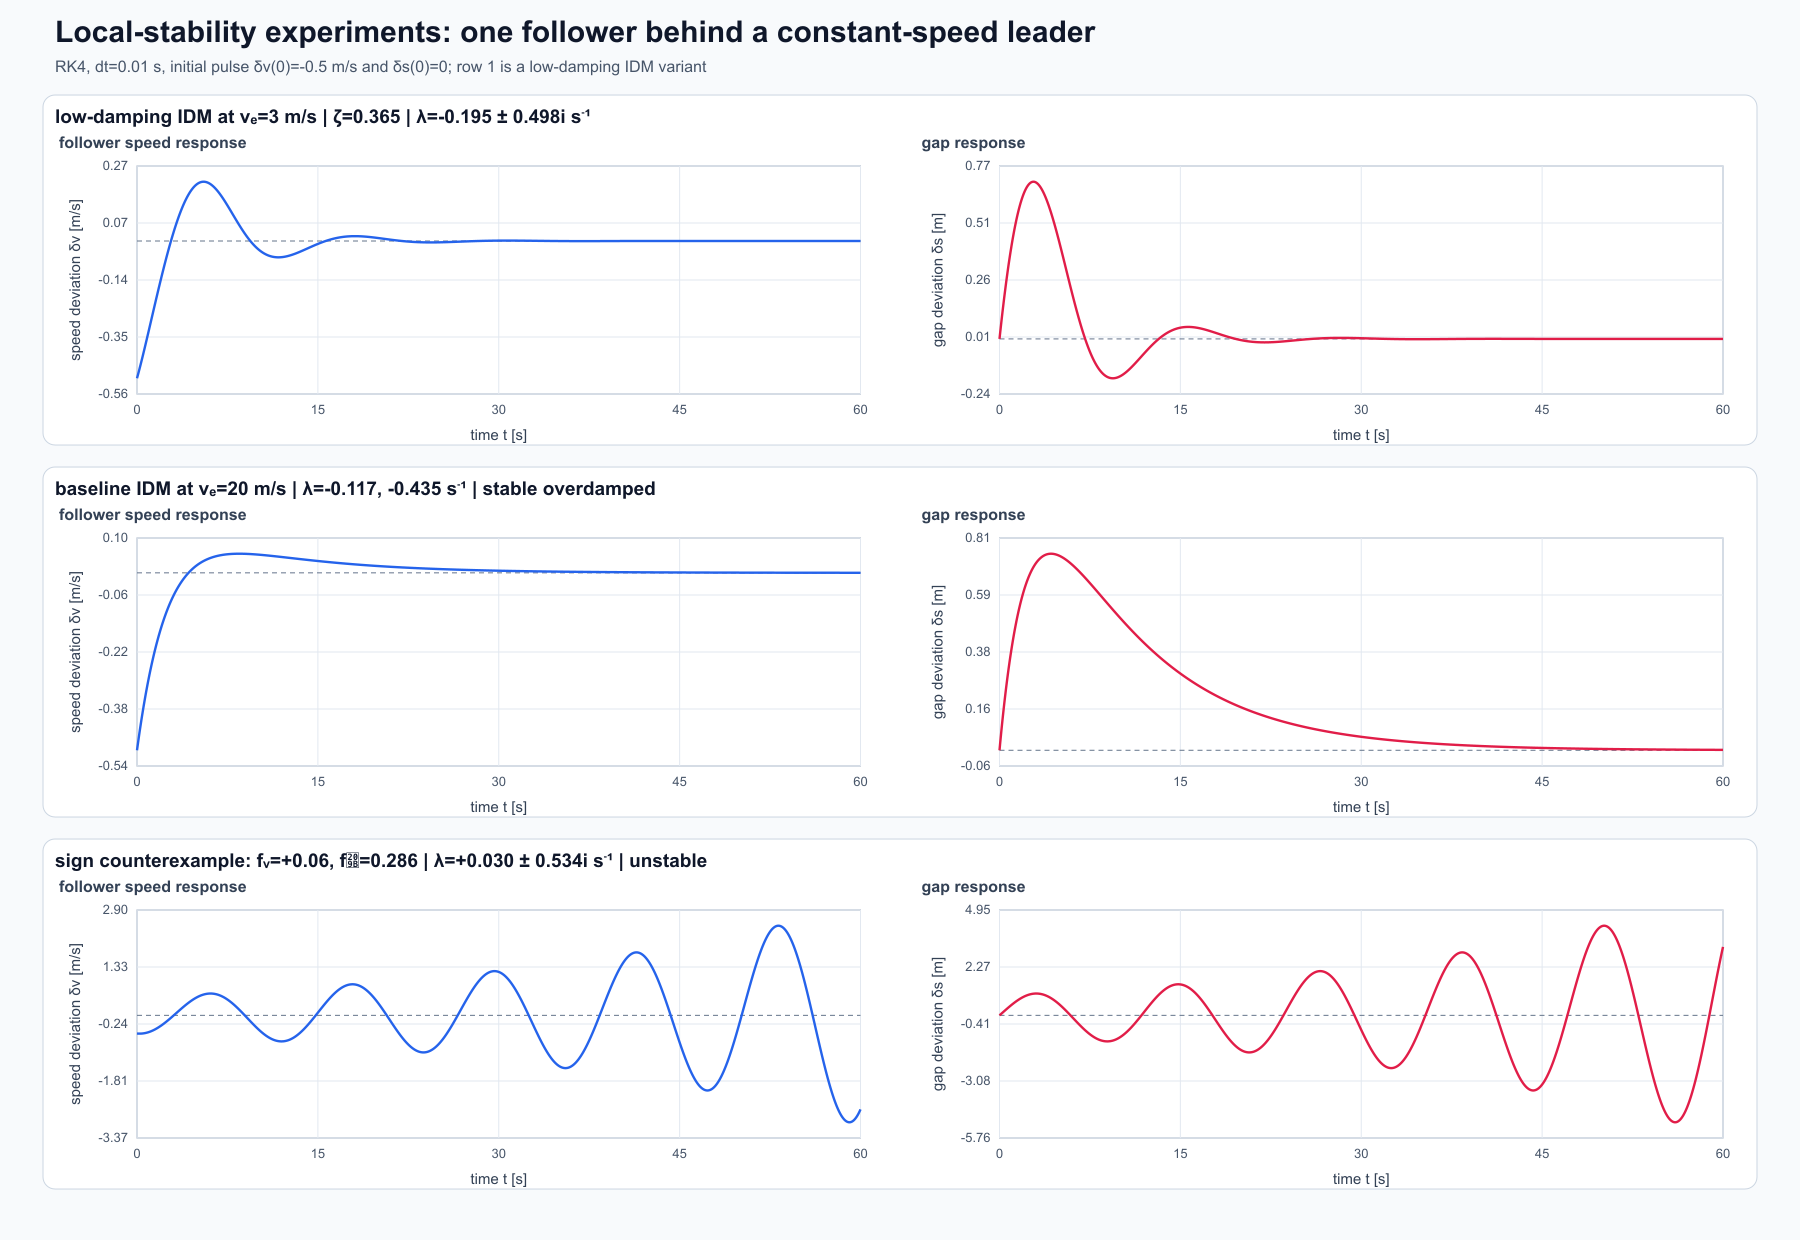
\includegraphics[width=\textwidth]{local_stability_experiments.png}
\caption{局部稳定性的三类单车响应。}
\label{fig:localexp}
\figurenote{局部稳定性的三种典型根型及其可观测响应。三行分别设置低阻尼 IDM、基准过阻尼 IDM 和 $f_v>0$ 的符号反例；左列是速度偏差，右列是净间距偏差，横线表示各自平衡值。第一行中速度和间距交替穿越平衡值，峰值绝对值逐次下降，说明两个特征根为实部负的共轭复根；这正是“稳定但欠阻尼”，超调本身并不代表失稳。第二行不再穿越或只出现很弱的穿越，两个负实根使恢复由慢根控制，展示过阻尼可以不振荡却恢复更慢。第三行峰谷包络随时间扩大，对应根的实部为正，证明即使恢复刚度 $f_s>0$，错误的速度阻尼符号仍足以造成局部失稳。三行的前车均保持匀速，所以该图证明的是单车能否回到给定平衡点，而不是车队扰动是否沿车辆编号放大；后一个问题必须由第~\ref{sec:string}~章的线稳定性分析回答。}
\end{figure}

\begin{tcolorbox}[resultbox,title=\textbf{局部试验的结论}]
局部稳定性只回答“这一辆车最终能不能恢复”。两个 IDM 工况都满足 $f_v<0$、$f_s>0$，因此都恢复；阻尼比与判别式决定恢复过程是否振荡。第一行有多次清晰超调，但包络持续减小，所以它仍然稳定。这个结论不能替代线稳定性：基准 IDM 在 $v_e=8$ m/s 时单车局部稳定，但同一工况放到长车队中，扰动仍会逐车放大，见图~\ref{fig:traj-s0}。
\end{tcolorbox}

\section{教学算例 M01：从特征根到 RK4 超调值}
\sectionstudy{experiment}{教学算例 M01：从特征根到 RK4 超调值}{wilsonward2011,ororsz2010}
\label{sub:m01-local}

取一个能手工核对的线性局部方程
\begin{equation}
\delta\ddot s+0.2\,\delta\dot s+0.25\,\delta s=0,
\qquad
\delta s(0)=1\ {\rm m},\quad \delta\dot s(0)=0.
\label{eq:m01-local}
\end{equation}
两根为
\[
\lambda_{1,2}=-0.1\pm0.489898\,\mathrm i,
\]
所以衰减时间为 $10$ s，阻尼振荡周期为
$2\pi/0.489898=12.8255$ s。解析解与 $\Delta t=0.05$ s 的 RK4 逐点比较，
最大绝对误差为 $6.01\times10^{-9}$ m；第一次反向超调为
$-0.52661$ m。图~\ref{fig:m01-local} 中曲线越过零点并不表示失稳，因为峰值包络仍按
$e^{-0.1t}$ 下降。

\begin{figure}[htbp]
\centering
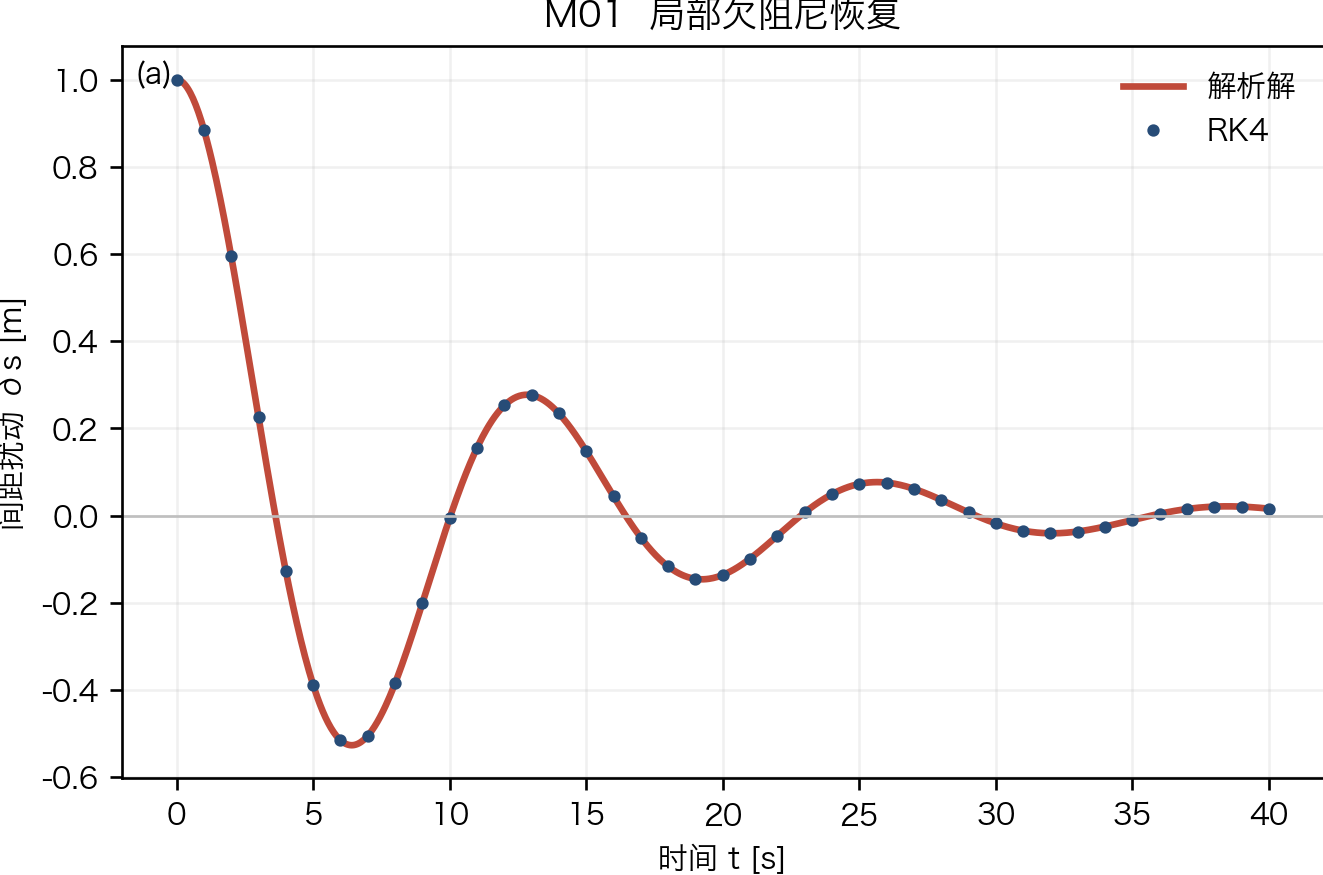
\includegraphics[width=0.86\textwidth]{mini_example_m01.png}
\caption{M01：局部欠阻尼响应。}
\label{fig:m01-local}
\figurenote{M01 手算例中同一局部二阶系统的解析解与 RK4 数值解。实线由特征根直接重构，离散圆点由逐步积分得到；两者在相位、第一次超调时刻和后续峰值上几乎重合，说明状态定义、加速度函数和 RK4 四个子步实现彼此一致。曲线第一次穿过零线后出现反向超调，随后正负峰值按指数包络衰减，这把“共轭复根”转化成了可直接识别的阻尼振荡。若数值点出现系统性的相位提前、峰值不衰减或与解析线分离，就意味着时间步过大或更新次序有误，而不是新的交通现象。该图因此同时证明两件事：欠阻尼稳定响应确实存在，并且本书后续仿真的时间积分器能正确再现该响应。}
\end{figure}

%==================================================================
\sectionwrapup{局部稳定只回答前车恢复匀速后某一辆跟车能否回到平衡。二阶根的实部决定衰减，虚部决定是否振荡；M01 进一步用解析解与 RK4 的 $6.01\times10^{-9}$ m 误差说明，明显超调仍然可以是稳定响应。局部稳定不能保证扰动沿整列车辆传播时不被放大。}

\chapter{线稳定性（String Stability）}
\label{sec:string}
\chapterguide{为什么每辆车都能恢复，扰动仍会沿车队放大}{本章从空间模态、长波展开和车对车传递函数三条路径建立线稳定判据，并系统解释幅值、波长、角频率、增长率和波速在理论与时空图中的对应关系。}

线稳定性回答的是：\textbf{扰动沿车队向上游传播时是放大还是衰减。}

\section{扰动的四个基本特征：幅值、波长、角频率与增长率}
\sectionstudy{theory}{扰动的四个基本特征：幅值、波长、角频率与增长率}{swaroop1996,stuedli2017,feng2019}
\label{sub:wavedef}

在线性分析中，一个实值速度扰动可写成
\begin{equation}
\boxed{
\delta v_n(t)
=A_0e^{\sigma t}
\cos\!\left(kn-\omega t+\phi\right)
}
\label{eq:waveform}
\end{equation}
或写成等价的复数形式
\begin{equation}
\delta v_n(t)
=\operatorname{Re}\!\left\{
A_0e^{i\phi}e^{(\sigma-i\omega)t+ikn}
\right\}.
\end{equation}
这个表达式把一个扰动拆成四个互不相同的特征：

\begin{center}
\small
\captionof{table}{扰动的幅值、波数、角频率与增长率。}
\label{tab:wave-quantities}
\begin{tabular}{p{2.4cm}p{2.4cm}p{4.4cm}p{4.5cm}}
\toprule
\textbf{特征} & \textbf{符号／单位} & \textbf{它控制什么} & \textbf{如何读取} \\
\midrule
幅值 & $A_0$，m/s & 初始扰动有多强 & 波峰相对平衡速度的最大偏差 \\[3pt]
空间波数 & $k$，rad/veh & 沿车辆序号变化有多快 & $k$ 越大，波长越短 \\[3pt]
角频率 & $\omega$，rad/s & 固定车辆看到的振荡有多快 & 周期 $T_\omega=2\pi/\omega$ \\[3pt]
增长率 & $\sigma$，s$^{-1}$ & 包络随时间放大还是衰减 & $\sigma>0$ 增长，$\sigma<0$ 衰减 \\
\bottomrule
\end{tabular}
\end{center}
\tabletext{tab:wave-quantities}{线性扰动的四个独立特征及其读法。幅值描述强弱，波数描述空间尺度，角频率描述时间振荡，增长率才决定包络放大或衰减；四者不能相互替代。}

在本书采用的复指数约定下，复特征值为
\begin{equation}
\lambda=\sigma-i\omega,
\qquad
\sigma=\operatorname{Re}\lambda,
\qquad
\omega=|\operatorname{Im}\lambda|.
\end{equation}
因此\textbf{角频率 $\omega$ 与空间波数 $k$ 不是同一个量}：$\omega$ 描述时间振荡，$k$ 描述空间起伏。两者由色散关系 $\lambda=\lambda(k)$ 联系起来。

\subsection{波数与波长}

若按车辆编号计量，一个完整空间周期所跨越的车辆数为
\begin{equation}
\Lambda_n=\frac{2\pi}{k}
\qquad\text{[veh]}.
\end{equation}
对 $N$ 辆车的环道，只允许
\begin{equation}
k_m=\frac{2\pi m}{N},
\qquad
\Lambda_n=\frac{N}{m},
\qquad
m=0,1,\ldots,N-1.
\end{equation}
$m$ 表示一圈内有多少个完整波。若平衡车头间距为 $s_e+l$，相应道路波长近似为
\begin{equation}
\Lambda_x=(s_e+l)\Lambda_n=\frac{L}{m}.
\end{equation}

例如 $N=120$、$v_e=8$ m/s 时，$s_e+l=19.0355$ m。主导模态 $m=4$ 对应
\begin{equation}
k_4=0.20944\ \text{rad/veh},
\qquad
\Lambda_n=30\ \text{veh},
\qquad
\Lambda_x\approx571.1\ \text{m}.
\end{equation}
也就是说，环道上同时出现 4 组波峰／波谷，每组波约跨 30 辆车。

\subsection{角频率、周期与相位速度}

固定观察第 $n$ 辆车时，式~\eqref{eq:waveform} 随时间重复的周期为
\begin{equation}
T_\omega=\frac{2\pi}{\omega},
\qquad
f=\frac{\omega}{2\pi}\quad\text{[Hz]}.
\end{equation}
保持相位 $kn-\omega t+\phi$ 不变，可得按车辆编号计的相位速度
\begin{equation}
c_n=\frac{\omega}{k}\quad\text{[veh/s]}.
\end{equation}
其正负取决于车辆编号方向与指数约定；转换为道路坐标下的波速时，还必须计入车辆平衡运动，因此本书最终以 $x$--$t$ 图中色带斜率或完整相位变换为准，不能简单把 $c_n$ 乘以车头间距就当作道路波速。

对上述 $m=4$ 算例，$|\operatorname{Im}\lambda|=0.12822$ rad/s，因此
\begin{equation}
T_\omega=49.00\ \text{s},
\qquad
|c_n|=\frac{0.12822}{0.20944}=0.6122\ \text{veh/s}.
\end{equation}
这意味着一辆固定探针车约每 49 s 经历一次同相位波动，而波峰在车辆序号方向上以约 $0.61$ 辆／秒移动。

\subsection{幅值为什么不进入线性稳定性判据}

线性方程满足比例叠加：若 $\delta v_n(t)$ 是解，则 $C\delta v_n(t)$ 也是解。因此在线性范围内，把初始幅值 $A_0$ 放大 10 倍，只会把整条响应曲线放大 10 倍，\textbf{不会改变} $\lambda(k)$、$\sigma$、$\omega$ 或临界参数。幅值演化为
\begin{equation}
A(t)=A_0e^{\sigma t}.
\end{equation}
例如基准 IDM 的 $m=4$ 模态在 $v_e=8$ m/s 时有 $\sigma=0.00408566$ s$^{-1}$。若 $A_0=0.002$ m/s，则在线性预测下
\begin{equation}
A(300)=0.002e^{0.00408566\times300}=0.00682\ \text{m/s}.
\end{equation}
改变 $A_0$ 不会改变指数斜率 $0.00408566$；但幅值大到使车辆接近停车、极小间距或加速度饱和后，非线性项开始起作用，增长不再严格服从指数律。所以所有定量稳定性实验都必须同时报告初始幅值与拟合时间窗。

\begin{tcolorbox}[notebox,title=\textbf{开链扫频与环道模态扫描在“扫描什么”}]
\begin{itemize}[leftmargin=1.4em,itemsep=3pt]
\item \textbf{开链传递函数实验：}人为给头车指定时间角频率 $\omega$，测量逐车幅值比 $|G(i\omega)|$ 与相位差；这里先扫描的是时间频率。
\item \textbf{环道特征值实验：}先指定离散空间波数 $k_m$，再由色散关系求 $\lambda_m=\sigma_m-i\omega_m$；这里先扫描的是空间波长。
\item 二者研究的是同一传播问题的两种切面。均匀单向模型中可由 $G(\lambda)=e^{ik}$ 相互转换；含双向耦合或异质性时，这种简单转换可能失效。
\end{itemize}
\end{tcolorbox}

\begin{tcolorbox}[experimentbox,title=\textbf{建议的三组扰动特征实验}]
\begin{enumerate}[leftmargin=1.6em,itemsep=3pt]
\item \textbf{波长扫描：}固定小幅值，依次注入 $m=1,2,\ldots,N/2$，比较实测增长率与 $\operatorname{Re}\lambda(k_m)$，定位最不稳定波长。
\item \textbf{角频率扫描：}在开链中令头车作不同 $\omega$ 的正弦扰动，测 $|Y_n/Y_{n-1}|$，画出放大频带。
\item \textbf{幅值扫描：}对同一 $k_m$ 使用 $A_0=0.002,0.02,0.2$ m/s。小幅值阶段三条 $\ln A(t)$ 曲线应平行；出现不平行时，说明已经离开线性范围。
\end{enumerate}
\end{tcolorbox}

\section{方法一：长波展开}
\sectionstudy{theory}{方法一：长波展开}{swaroop1996,stuedli2017,feng2019}

改用位置扰动 $y_n = \delta x_n$，则 $\delta s_n = y_{n-1}-y_n$、$\delta v_n = \dot y_n$：
\begin{equation}
\ddot y_n = f_s\left(y_{n-1}-y_n\right) + f_v\,\dot y_n + f_{v_l}\,\dot y_{n-1}
\end{equation}

设行波解 $y_n(t) = \hat y\,e^{\lambda t + ikn}$，于是 $y_{n-1}=y_n e^{-ik}$，得色散关系
\begin{equation}
\lambda^2 = f_s\left(e^{-ik}-1\right) + \left(f_v + f_{v_l}e^{-ik}\right)\lambda
\label{eq:disp}
\end{equation}

失稳最先出现在长波（$k\to 0$）。令 $\varepsilon = -ik$，展开 $\lambda = c_1\varepsilon + c_2\varepsilon^2 + \cdots$，并利用 $e^{\varepsilon}=1+\varepsilon+\tfrac{\varepsilon^2}{2}+\cdots$，逐阶匹配：

\textbf{$O(\varepsilon)$ 阶：}
\begin{equation}
0 = f_s + \left(f_v+f_{v_l}\right)c_1
\qquad\Longrightarrow\qquad
c_1 = -\frac{f_s}{f_v+f_{v_l}} = V'(s_e)
\end{equation}
即 $c_1$ 就是运动学波速，与式~\eqref{eq:Vprime} 一致。

\textbf{$O(\varepsilon^2)$ 阶：}
\begin{equation}
c_1^2 = \frac{f_s}{2} + f_{v_l}c_1 + \left(f_v+f_{v_l}\right)c_2
\qquad\Longrightarrow\qquad
c_2 = \frac{c_1^2 - \frac12 f_s - f_{v_l}c_1}{f_v+f_{v_l}}
\end{equation}

由 $\lambda = -i c_1 k - c_2 k^2$ 知 $\operatorname{Re}\lambda = -c_2 k^2$，稳定要求 $c_2\ge 0$。因分母 $f_v+f_{v_l}<0$，故须分子非正：
\begin{equation}
c_1^2 - \tfrac12 f_s - f_{v_l}c_1 \le 0
\end{equation}

代入 $c_1$ 并同乘 $\left(f_v+f_{v_l}\right)^2/f_s > 0$：
\begin{equation}
f_s + f_{v_l}\left(f_v+f_{v_l}\right) - \tfrac12\left(f_v+f_{v_l}\right)^2 \le 0
\end{equation}

注意到
\begin{equation}
f_{v_l}\left(f_v+f_{v_l}\right) - \tfrac12\left(f_v+f_{v_l}\right)^2
= \left(f_v+f_{v_l}\right)\cdot\frac{f_{v_l}-f_v}{2}
= \frac{f_{v_l}^2 - f_v^2}{2}
\end{equation}

于是得到
\begin{tcolorbox}[keybox,title=\textbf{线稳定性条件（长波）}]
\begin{equation}
\frac{1}{2}\left(f_v^2 - f_{v_l}^2\right) \;\ge\; f_s
\label{eq:string}
\end{equation}
\end{tcolorbox}

\subsection{为什么原始跟驰模型首先发生长波失稳}
\label{sub:why-long-wave-first}

“首先长波失稳”并不是由仿真图像猜出来的，而是由 $k=0$ 附近的谱结构决定。令
\begin{equation}
\mu=f_v+f_{v_l}<0,
\qquad
\Phi=\frac{f_v^2-f_{v_l}^2}{2}-f_s .
\end{equation}
把 $k=0$ 代入色散关系~\eqref{eq:disp}，得到
\begin{equation}
\lambda(\lambda-\mu)=0,
\qquad
\lambda_0=0,\qquad \lambda_f=\mu<0 .
\label{eq:k0roots}
\end{equation}
其中 $\lambda_f$ 是快速衰减的单车松弛模态；$\lambda_0=0$ 则来自平移不变性：把环上所有车辆的位置整体平移同一个常量，不会改变任何间距或加速度，所以系统必须有一个既不增长也不衰减的零根。长波分支正是从这个零根连续伸出来，因此它天然贴近虚轴，最容易在参数变化时首先越过稳定边界。

把前面的 $c_2$ 进一步整理，可得
\begin{equation}
c_2=-\frac{f_s}{\mu^3}\,\Phi,
\qquad
\lambda(k)=-ic_1k-c_2k^2+O(k^3),
\qquad
c_1=-\frac{f_s}{\mu}=V'(s_e).
\label{eq:longwave-branch}
\end{equation}
由于 $\mu^3<0$，系数 $-f_s/\mu^3>0$，所以 $c_2$ 与 $\Phi$ 同号：
\begin{equation}
\Phi>0\Rightarrow\operatorname{Re}\lambda\simeq-c_2k^2<0,
\qquad
\Phi<0\Rightarrow\operatorname{Re}\lambda\simeq-c_2k^2>0.
\end{equation}
一旦 $\Phi$ 从正变负，任意足够小但非零的 $k$ 都立即获得正增长率。严格地说，\textbf{不是 $k=0$ 本身失稳}；$k=0$ 仍是中性的整体平移，而是 $k\to0$、$k\ne0$ 的长波分支最先进入右半平面。

这个结论也可写成等效的长波偏微分方程。若 $r(n,t)$ 表示缓慢变化的间距扰动，则线性主部为
\begin{equation}
r_t+c_1r_n=c_2r_{nn}+\cdots .
\label{eq:effective-diffusion}
\end{equation}
$c_1$ 只负责把扰动搬运；$c_2>0$ 时，$r_{nn}$ 像正常扩散一样抹平起伏；$c_2<0$ 时则成为“反扩散”，宽而缓的起伏会被放大。相邻车辆对长波的差值只有
\begin{equation}
e^{-ik}-1=-ik-\frac{k^2}{2}+O(k^3),
\end{equation}
恢复与耗散信号都很弱，净阻尼仅为 $O(k^2)$；短波中相邻车辆差异是 $O(1)$，局部速度阻尼更容易把它压下去。这就是长波在物理上更危险的原因。

\begin{tcolorbox}[notebox,title=\textbf{有限环道为什么可能“看不见”这一失稳}]
环道只允许 $k_m=2\pi m/N$。最危险的连续长波在 $k\to0$，但有限车辆数能取到的最小非零波数是 $k_{\min}=2\pi/N$；若 $N$ 太小，第一个离散点可能已经跳过正增长率区间，于是仿真会把本来不稳定的无限车队误判为稳定。第~\ref{sec:appx}~章的 E5 正是对此效应的定量检验。
\end{tcolorbox}

\subsection{教学算例 M02：同一 IDM，为什么 12 辆稳定而 20 辆失稳}
\label{sub:m02-finite-ring}

固定原始 IDM 与 $v_e=8$ m/s，只改变环道车辆数。对每个允许波数
$k_m=2\pi m/N$ 求两根并取最大实部：
\begin{center}
\small
\captionof{table}{M02 不同车辆数下的最低离散模态。}
\label{tab:m02-finite-ring}
\begin{tabular}{rccc}
\toprule
$N$ & 主导模态 $m^*$ & 波长 [辆] & $\max\operatorname{Re}\lambda$ [s$^{-1}$] \\
\midrule
12 & 1 & 12 & $-0.0210366$ \\
20 & 1 & 20 & $+0.00130121$ \\
30 & 1 & 30 & $+0.00408566$ \\
\bottomrule
\end{tabular}
\end{center}
\tabletext{tab:m02-finite-ring}{同一 IDM 工作点在 $N=12,20,30$ 时允许的主导波长与增长率。车辆数从 12 增至 20 后最低非零波数进入长波失稳区，因此有限环道稳定不能直接推出无限车队稳定。}
同一套参数在 $N=12$ 时，第一个非零波数仍落在负增长区；到 $N=20$，
$k_{\min}$ 足够靠近零，终于采样到正增长长波。因此“12 辆环道没有出现走停波”
不能推出无限车队稳定，只能推出该小环道的\textbf{三个允许模态}均未增长。

\begin{figure}[htbp]
\centering
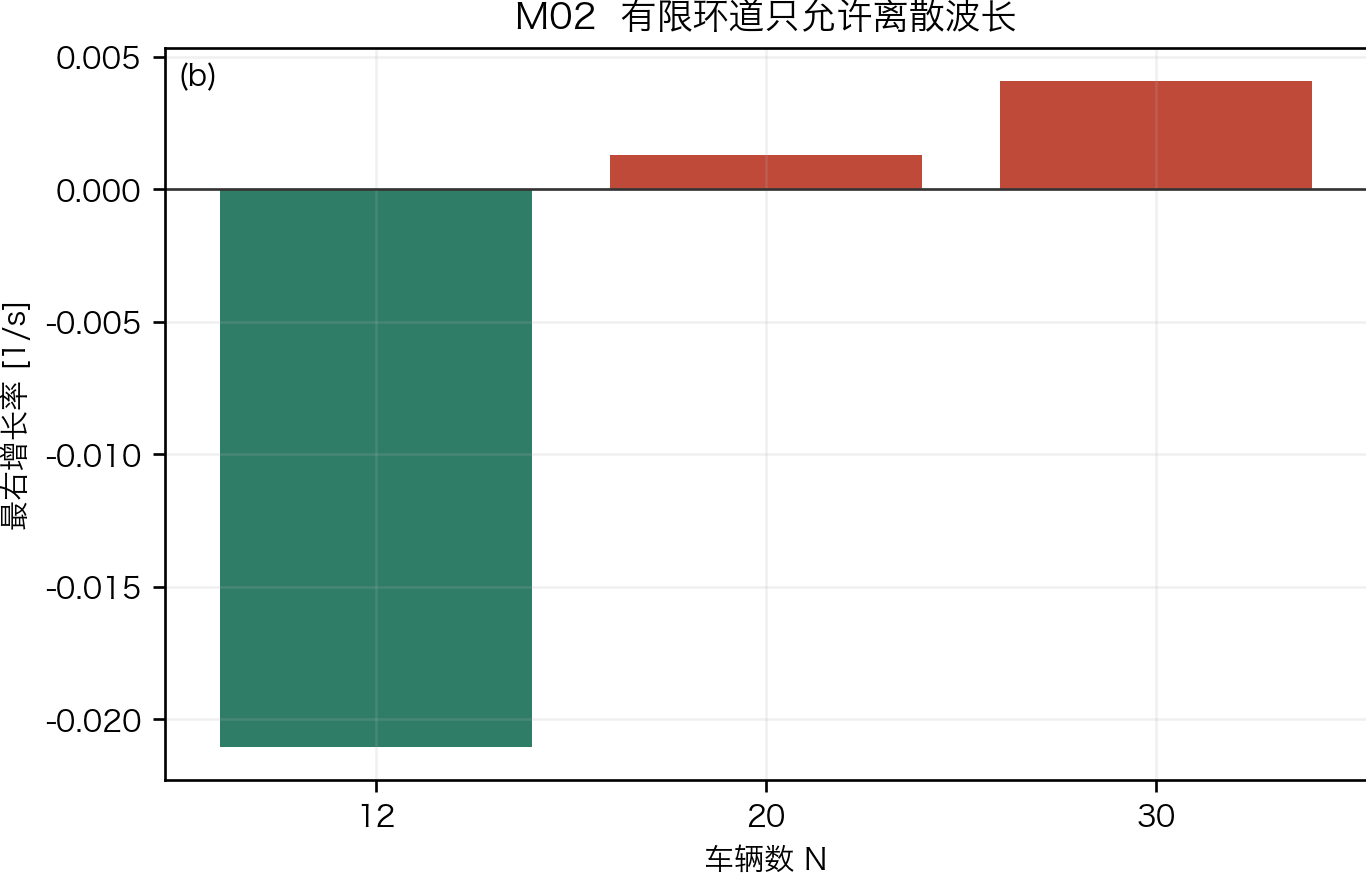
\includegraphics[width=0.82\textwidth]{mini_example_m02.png}
\caption{M02：有限环道的离散波长效应。}
\label{fig:m02-finite-ring}
\figurenote{M02 对有限环道离散模态的逐一谱检验。每根柱对应 $k_m=2\pi m/N$ 的最右特征根实部，绿色表示该模态衰减，红色表示随时间增长；不同面板只改变车辆数 $N$，IDM 参数和平衡工作点完全相同。小环道的最低非零波数较大，危险的极长波无法满足周期闭合，所以全部可用柱可能仍为绿色；随着 $N$ 增大，$k_{min}=2\pi/N$ 向零移动，首先出现的红柱正是最低阶长波。该现象证明有限环道并不是无限车队判据的无偏缩小版：它会因为缺少足够长的波长而系统性高估稳定性。图中红柱出现的位置还给出了即将主导时域走停波的车辆尺度，因此实验报告应同时写明 $N$，不能只报告密度和 IDM 参数。}
\end{figure}

\begin{tcolorbox}[notebox,title=\textbf{适用边界：并非所有扩展模型都先失去长波稳定}]
上述“首先长波失稳”对本书的\textbf{原始、均匀、单向、无延迟}模型成立，而且下一节的传递函数会证明最危险频率确为 $\omega\to0$。当前车加速度增益过强、存在回望耦合、时间延迟或离散控制时，有限波长／有限频率分支可能先越过虚轴；此时必须扫描全波数或全频段，不能只检查式~\eqref{eq:string}。
\end{tcolorbox}

\section{方法二：传递函数法}
\sectionstudy{theory}{方法二：传递函数法}{swaroop1996,ploeg2014,feng2019}

长波展开只保证 $k\to0$ 邻域内衰减。要断定\textbf{所有波长}的扰动都不放大，需要频域方法。本小节把每一步写全。

\subsection{第一步：为什么可以做 Laplace 变换}

线性化后的位置扰动方程
\begin{equation}
\ddot y_n = f_s\left(y_{n-1}-y_n\right) + f_v\,\dot y_n + f_{v_l}\,\dot y_{n-1}
\label{eq:ylin}
\end{equation}
是\textbf{常系数}线性微分方程（系数 $f_s,f_v,f_{v_l}$ 都是在平衡点求的常数），且对每个 $n$ 结构完全相同。这两点保证了 Laplace 变换可用、且变换后的输入输出比与车号 $n$ 无关。

设扰动前车队处于平衡态，取零初始条件
\begin{equation}
y_n(0) = 0, \qquad \dot y_n(0) = 0 \qquad \forall n
\end{equation}
记 $Y_n(\lambda) = \mathcal{L}\{y_n(t)\} = \int_0^\infty y_n(t)\,e^{-\lambda t}\,\mathrm{d}t$。零初始条件下微分的变换法则为
\begin{equation}
\mathcal{L}\{\dot y_n\} = \lambda Y_n - y_n(0) = \lambda Y_n,
\qquad
\mathcal{L}\{\ddot y_n\} = \lambda^2 Y_n - \lambda y_n(0) - \dot y_n(0) = \lambda^2 Y_n
\end{equation}

\subsection{第二步：变换并整理出传递函数}

对式~\eqref{eq:ylin} 两边逐项变换：
\begin{equation}
\lambda^2 Y_n = f_s\left(Y_{n-1}-Y_n\right) + f_v\,\lambda Y_n + f_{v_l}\,\lambda Y_{n-1}
\end{equation}

把含 $Y_n$ 的项全部移到左边、含 $Y_{n-1}$ 的项移到右边：
\begin{equation}
\lambda^2 Y_n + f_s Y_n - f_v\lambda Y_n = f_s Y_{n-1} + f_{v_l}\lambda Y_{n-1}
\end{equation}

两边分别提取公因子：
\begin{equation}
\left(\lambda^2 - f_v\lambda + f_s\right) Y_n = \left(f_{v_l}\lambda + f_s\right) Y_{n-1}
\end{equation}

作商即得\textbf{车对车传递函数}：
\begin{tcolorbox}[keybox,title=\textbf{车对车传递函数}]
\begin{equation}
G(\lambda) \;=\; \frac{Y_n(\lambda)}{Y_{n-1}(\lambda)}
\;=\; \frac{f_s + f_{v_l}\lambda}{\lambda^2 - f_v\lambda + f_s}
\label{eq:G0}
\end{equation}
\end{tcolorbox}

三点观察：

\begin{itemize}[leftmargin=1.4em,itemsep=3pt]
\item \textbf{分母恰好是局部稳定性的特征多项式}（见式~\eqref{eq:char}）。所以局部稳定 $\iff$ $G$ 的极点都在左半平面 $\iff$ $G$ 本身是稳定传递函数。这是讨论 $\left|G\right|$ 有意义的前提：若 $G$ 不稳定，单车响应已经发散，谈"扰动放大倍数"没有意义。
\item \textbf{$G$ 与 $n$ 无关}（车队均匀），所以扰动逐级相乘：
\begin{equation}
Y_n = G(\lambda)\,Y_{n-1} = G^2(\lambda)\,Y_{n-2} = \cdots = G^{\,n}(\lambda)\,Y_0
\end{equation}
\item \textbf{位置、速度、间距共用同一个 $G$。} 速度扰动 $\mathcal{L}\{\delta v_n\} = \lambda Y_n$，作商时 $\lambda$ 约掉；间距扰动 $\mathcal{L}\{\delta s_n\} = Y_{n-1}-Y_n$，则
\[
\frac{\mathcal{L}\{\delta s_{n+1}\}}{\mathcal{L}\{\delta s_n\}}
= \frac{Y_n - Y_{n+1}}{Y_{n-1}-Y_n}
= \frac{G\left(Y_{n-1}-Y_n\right)}{Y_{n-1}-Y_n} = G
\]
所以不必区分用哪个变量定义线稳定。
\end{itemize}

\subsection{第三步：判据为什么是 $\left|G(i\omega)\right|\le1$}

由 $Y_n = G^{\,n}Y_0$，取 $\lambda = i\omega$（即考察频率为 $\omega$ 的正弦扰动的稳态响应）：
\begin{equation}
\left|Y_n(i\omega)\right| = \left|G(i\omega)\right|^{\,n}\left|Y_0(i\omega)\right|
\end{equation}

于是：若存在某个频率 $\omega^\star$ 使 $\left|G(i\omega^\star)\right|>1$，该频率分量沿车队\textbf{按几何级数放大}，往上游传若干辆车后必然超出线性范围，长成走停波。反之若所有频率的增益都不超过 1，任何扰动（按 Fourier 分解为各频率之和）都不会被放大。

\begin{tcolorbox}[keybox,title=\textbf{线稳定性的严格定义}]
\[
\text{线稳定}
\iff
\left\|G\right\|_{\infty} \equiv \sup_{\omega\in\mathbb{R}}\left|G(i\omega)\right| \;\le\; 1
\quad\text{且}\quad G\ \text{稳定（局部稳定）}
\]
\end{tcolorbox}

\subsection{第四步：计算 $\left|G(i\omega)\right|^2$}

把 $\lambda = i\omega$ 代入式~\eqref{eq:G0}，分子分母分别拆成实部与虚部。

\textbf{分子.}
\begin{equation}
N(i\omega) = f_s + f_{v_l}\,(i\omega) = \underbrace{f_s}_{\text{实部}} + i\underbrace{f_{v_l}\omega}_{\text{虚部}}
\qquad\Longrightarrow\qquad
\left|N\right|^2 = f_s^2 + f_{v_l}^2\omega^2
\end{equation}

\textbf{分母.} 注意 $(i\omega)^2 = i^2\omega^2 = -\omega^2$：
\begin{equation}
D(i\omega) = (i\omega)^2 - f_v(i\omega) + f_s
= \underbrace{\left(f_s-\omega^2\right)}_{\text{实部}} + i\underbrace{\left(-f_v\omega\right)}_{\text{虚部}}
\end{equation}
\begin{equation}
\left|D\right|^2 = \left(f_s-\omega^2\right)^2 + f_v^2\omega^2
\end{equation}

（虚部取平方，负号消失，故写成 $f_v^2\omega^2$。）

于是
\begin{equation}
\left|G(i\omega)\right|^2 = \frac{\left|N\right|^2}{\left|D\right|^2}
= \frac{f_s^2 + f_{v_l}^2\omega^2}{\left(f_s-\omega^2\right)^2 + f_v^2\omega^2}
\end{equation}

条件 $\left|G\right|\le1$ 等价于 $\left|G\right|^2\le1$，即 $\left|N\right|^2\le\left|D\right|^2$：
\begin{tcolorbox}[keybox,title=\textbf{幅值条件}]
\begin{equation}
f_s^2 + f_{v_l}^2\omega^2
\;\le\;
\left(f_s-\omega^2\right)^2 + f_v^2\omega^2
\end{equation}
\end{tcolorbox}

\subsection{第五步：化简}

移项，把左边减到右边：
\begin{equation}
\left|D\right|^2 - \left|N\right|^2
= \underbrace{f_s^2 - 2f_s\omega^2 + \omega^4}_{\left(f_s-\omega^2\right)^2} + f_v^2\omega^2 - f_s^2 - f_{v_l}^2\omega^2 \;\ge\; 0
\end{equation}

$f_s^2$ 相消，其余每项都含 $\omega^2$，提出公因子：
\begin{equation}
\omega^2\left[\omega^2 - 2f_s + f_v^2 - f_{v_l}^2\right] \;\ge\; 0
\label{eq:bracket}
\end{equation}

因 $\omega^2\ge0$ 恒成立，条件归结为方括号非负。方括号是 $\omega^2$ 的\textbf{单调增}函数，最小值在 $\omega\to0$ 取得，故对一切 $\omega$ 成立当且仅当
\begin{equation}
f_v^2 - f_{v_l}^2 - 2f_s \;\ge\; 0
\end{equation}

即式~\eqref{eq:string}。这同时说明该条件是\textbf{充要}的，且\textbf{最危险频率是 $\omega\to0$}——与长波展开的结论互相印证。

\begin{tcolorbox}[notebox,title=\textbf{为什么 $\omega=0$ 处总是取等号}]
式~\eqref{eq:bracket} 在 $\omega=0$ 处恒为 0，对应 $\left|G(0)\right| = f_s/f_s = 1$。这不是巧合：$\lambda=0$ 表示"把所有车的位置整体平移一个常量"，这本身就是一个合法的新平衡态，既不放大也不衰减。所以 $\left|G\right|$ 曲线永远从 1 出发，稳定与否取决于它\textbf{离开 1 之后是向下还是向上}。对小 $\omega$ 作展开：
\[
\left|G(i\omega)\right|^2 \approx 1 + \frac{2f_s + f_{v_l}^2 - f_v^2}{f_s^2}\,\omega^2 + O(\omega^4)
\]
$\omega^2$ 系数为负即稳定，正是同一个条件。
\end{tcolorbox}

\subsection{补充：传递函数与色散关系的等价性}

两种方法本质是同一件事。把式~\eqref{eq:disp} 的色散关系整理：
\begin{equation}
\left(\lambda^2 - f_v\lambda + f_s\right) = e^{-ik}\left(f_s + f_{v_l}\lambda\right)
\qquad\Longleftrightarrow\qquad
G(\lambda) = e^{\,ik}
\end{equation}

即：\textbf{色散关系就是方程 $G(\lambda)=e^{ik}$}。中性稳定曲线 $\operatorname{Re}\lambda=0$ 对应 $\left|G\right|=1$。长波展开是在 $k\to0$ 处解这个方程，传递函数法则是直接扫描整条 $\lambda=i\omega$ 轴——后者更全面，这一点在第~\ref{sec:lead}~章含前车加速度时会变得关键。

\section{用原始偏导表示}
\sectionstudy{theory}{用原始偏导表示}{swaroop1996,stuedli2017,feng2019}

代回 $f_v = F_v+F_{\dv}$、$f_{v_l}=-F_{\dv}$：
\begin{tcolorbox}[keybox]
\begin{equation}
\frac{1}{2}F_v^2 + F_v F_{\dv} - F_s \;\ge\; 0
\end{equation}
\end{tcolorbox}

注意 $F_v<0$ 且 $F_{\dv}<0$，故 $F_vF_{\dv}>0$：\textbf{相对速度反馈项总是起稳定作用。}

\begin{tcolorbox}[notebox,title=\textbf{校验：退化到 OVM}]
最优速度模型 $\dot v = \left[V(s)-v\right]/\tau$ 有 $F_s = V'/\tau$、$F_v=-1/\tau$、$F_{\dv}=0$，条件退化为
\[
V'(s_e) \le \frac{1}{2\tau}
\]
与经典结果一致。
\end{tcolorbox}

%==================================================================
\sectionwrapup{线稳定性要求任意频率的扰动在逐车传递时不放大，等价地要求环道所有非平凡空间模态不增长。幅值、角频率、波长、相速和增长率分别描述不同观测；长波门槛由 $k\to0$ 展开得到，有限车数只抽样离散波数。}

\chapter{代入 IDM}
\label{sec:idm}
\chapterguide{一般判据如何变成可计算的 IDM 稳定域}{本章计算 IDM 平衡关系与偏导，把抽象条件化为速度、密度和模型参数的函数。读者应掌握从参数到中性边界的计算链条，并理解“参数物理合理”不等于“全工况线稳定”。}

\section{模型与平衡态}
\sectionstudy{model}{模型与平衡态}{treiber2000,sugiyama2008,treiberkesting2013}

\begin{equation}
\dot v = a\left[1 - \left(\frac{v}{v_0}\right)^{\delta} - \left(\frac{s^*(v,\dv)}{s}\right)^{2}\right],
\qquad
s^* = s_0 + vT + \frac{v\,\dv}{2\sqrt{ab}}
\end{equation}

平衡时 $\dv=0$，故 $s_e^* = s_0+v_eT$。令 $\dot v=0$：
\begin{equation}
\left(\frac{s_e^*}{s_e}\right)^2 = 1-\left(\frac{v_e}{v_0}\right)^{\delta}
\qquad\Longrightarrow\qquad
s_e(v_e) = \frac{s_0+v_eT}{\sqrt{1-\left(v_e/v_0\right)^{\delta}}}
\end{equation}

记
\begin{equation}
z \equiv \frac{s_e^*}{s_e} = \sqrt{1-\left(\frac{v_e}{v_0}\right)^{\delta}} \in (0,1]
\end{equation}

\section{三个偏导数}
\sectionstudy{theory}{三个偏导数}{treiber2000,sugiyama2008,treiberkesting2013}

\begin{align}
F_s &= \frac{2a\left(s_e^*\right)^2}{s_e^3} = \frac{2az^2}{s_e} \\[6pt]
F_v &= -\underbrace{\frac{a\delta}{v_0}\left(\frac{v_e}{v_0}\right)^{\delta-1}}_{\textstyle A}
       \;-\;\underbrace{\frac{2azT}{s_e}}_{\textstyle B}
       \qquad\left(\text{因 } \left.\frac{\partial s^*}{\partial v}\right|_e = T\right) \\[6pt]
F_{\dv} &= -\frac{2a\,s_e^*}{s_e^2}\cdot\frac{v_e}{2\sqrt{ab}}
       = -\underbrace{\sqrt{\frac{a}{b}}\,\frac{z\,v_e}{s_e}}_{\textstyle C}
\end{align}

\section{IDM 的稳定性条件}
\sectionstudy{model}{IDM 的稳定性条件}{treiber2000,treiberkesting2013}

\textbf{局部稳定性.} $F_s>0$ 且 $f_v = F_v+F_{\dv} = -(A+B+C)<0$。只要 $v_e<v_0$（即 $z>0$），两者恒成立。

\begin{tcolorbox}[notebox]
\textbf{IDM 在整个平衡分支上永远局部稳定}，只是当 $(A+B+C)^2<4F_s$ 时为欠阻尼，表现为衰减振荡。
\end{tcolorbox}

\textbf{线稳定性.}
\begin{tcolorbox}[keybox,title=\textbf{IDM 线稳定性判据}]
\begin{equation}
\Phi(v_e) \equiv \frac{1}{2}(A+B)^2 + (A+B)\,C - F_s \;\ge\; 0
\label{eq:idmphi}
\end{equation}
其中
\[
A = \frac{a\delta}{v_0}\left(\frac{v_e}{v_0}\right)^{\delta-1},
\qquad
B = \frac{2azT}{s_e},
\qquad
C = \sqrt{\frac{a}{b}}\,\frac{z\,v_e}{s_e}
\]
\[
z = \sqrt{1-\left(v_e/v_0\right)^{\delta}},
\qquad
s_e = \frac{s_0+v_eT}{z}
\]
\end{tcolorbox}

\section{两个极限}
\sectionstudy{theory}{两个极限}{treiber2000,sugiyama2008,treiberkesting2013}

\textbf{自由流极限 $v_e\to v_0$.} 此时 $z\to 0$，$F_s\to 0$、$B\to 0$、$C\to 0$，而 $A$ 保持有限正值，故 $\Phi\to\tfrac12A^2>0$：\textbf{恒线稳定}。

\textbf{拥堵极限 $v_e\to 0$.} 此时 $z\to1$、$s_e\to s_0$、$A\to0$（$\delta>1$）、$C\to0$、$B\to 2aT/s_0$，条件化为
\begin{equation}
\frac{1}{2}\left(\frac{2aT}{s_0}\right)^2 \ge \frac{2a}{s_0}
\qquad\Longleftrightarrow\qquad
\frac{aT^2}{s_0} \ge 1
\end{equation}

这解释了为何 IDM 在停走交通附近对 $T$、$a$、$s_0$ 极其敏感。

%==================================================================
\sectionwrapup{将 IDM 的平衡关系和三个偏导代入一般判据，可得到随速度变化的局部与线稳定边界。低速极限显示 $T$、$a$、$s_0$ 直接控制稳定裕度；参数物理上合理并不意味着所有密度下都线稳定。}

\chapter{数值算例}
\label{sec:num}
\chapterguide{理论预测如何由可复现实验验证}{本章在统一参数下并列稳定与失稳工况，用增长率、主导模态、位置--时间速度着色轨迹以及指定车辆速度／间距曲线交叉验证理论，建立全书后续算例的读图标准。}

\begin{center}
\captionof{table}{全书数值实验采用的基准 IDM 参数。}
\label{tab:baseline-idm-parameters}
\begin{tabular}{lcccccccc}
\toprule
参数 & $v_0$ & $T$ & $s_0$ & $a$ & $b$ & $\delta$ & $l$ \\
\midrule
取值 & 33.3 m/s & 1.5 s & 2 m & 1 m/s$^2$ & 1.5 m/s$^2$ & 4 & 5 m \\
\bottomrule
\end{tabular}
\end{center}
\tabletext{tab:baseline-idm-parameters}{期望速度、时距、最小间距、加减速度和车长的统一基准值。后续场景若未特别说明均沿用这些参数，因此不同机制之间的比较不会混入参数配方变化。}

将式~\eqref{eq:idmphi} 在全速域扫描，得两个临界点：

\begin{center}
\captionof{table}{基准 IDM 不稳定速度带的两个临界工作点。}
\label{tab:idm-critical-points}
\begin{tabular}{lccccc}
\toprule
临界点 & $v_e$ & $s_e$ & 车头间距 $s_e+l$ & 密度 $\rho$ & 流量 $Q$ \\
\midrule
下临界 & 0.91 m/s & 3.36 m & 8.36 m & 119.6 veh/km & 391 veh/h \\
上临界 & 18.61 m/s & 31.50 m & 36.50 m & 27.4 veh/km & 1836 veh/h \\
\bottomrule
\end{tabular}
\end{center}
\tabletext{tab:idm-critical-points}{下、上临界点对应的速度、间距、密度与流量。它把速度域中的解析稳定边界转换为道路运行指标，并显示上临界点已接近基本图容量区域。}

\begin{tcolorbox}[notebox,title=\textbf{线不稳定区间}]
\[
v_e \in (0.91,\; 18.61)\ \text{m/s}
\qquad\text{即约}\qquad
3.3\text{--}67\ \text{km/h}
\]
判据函数最小值 $\Phi_{\min}=-0.027$，出现在 $v_e\approx 3.1$ m/s。
\end{tcolorbox}

\begin{figure}[htbp]
\centering
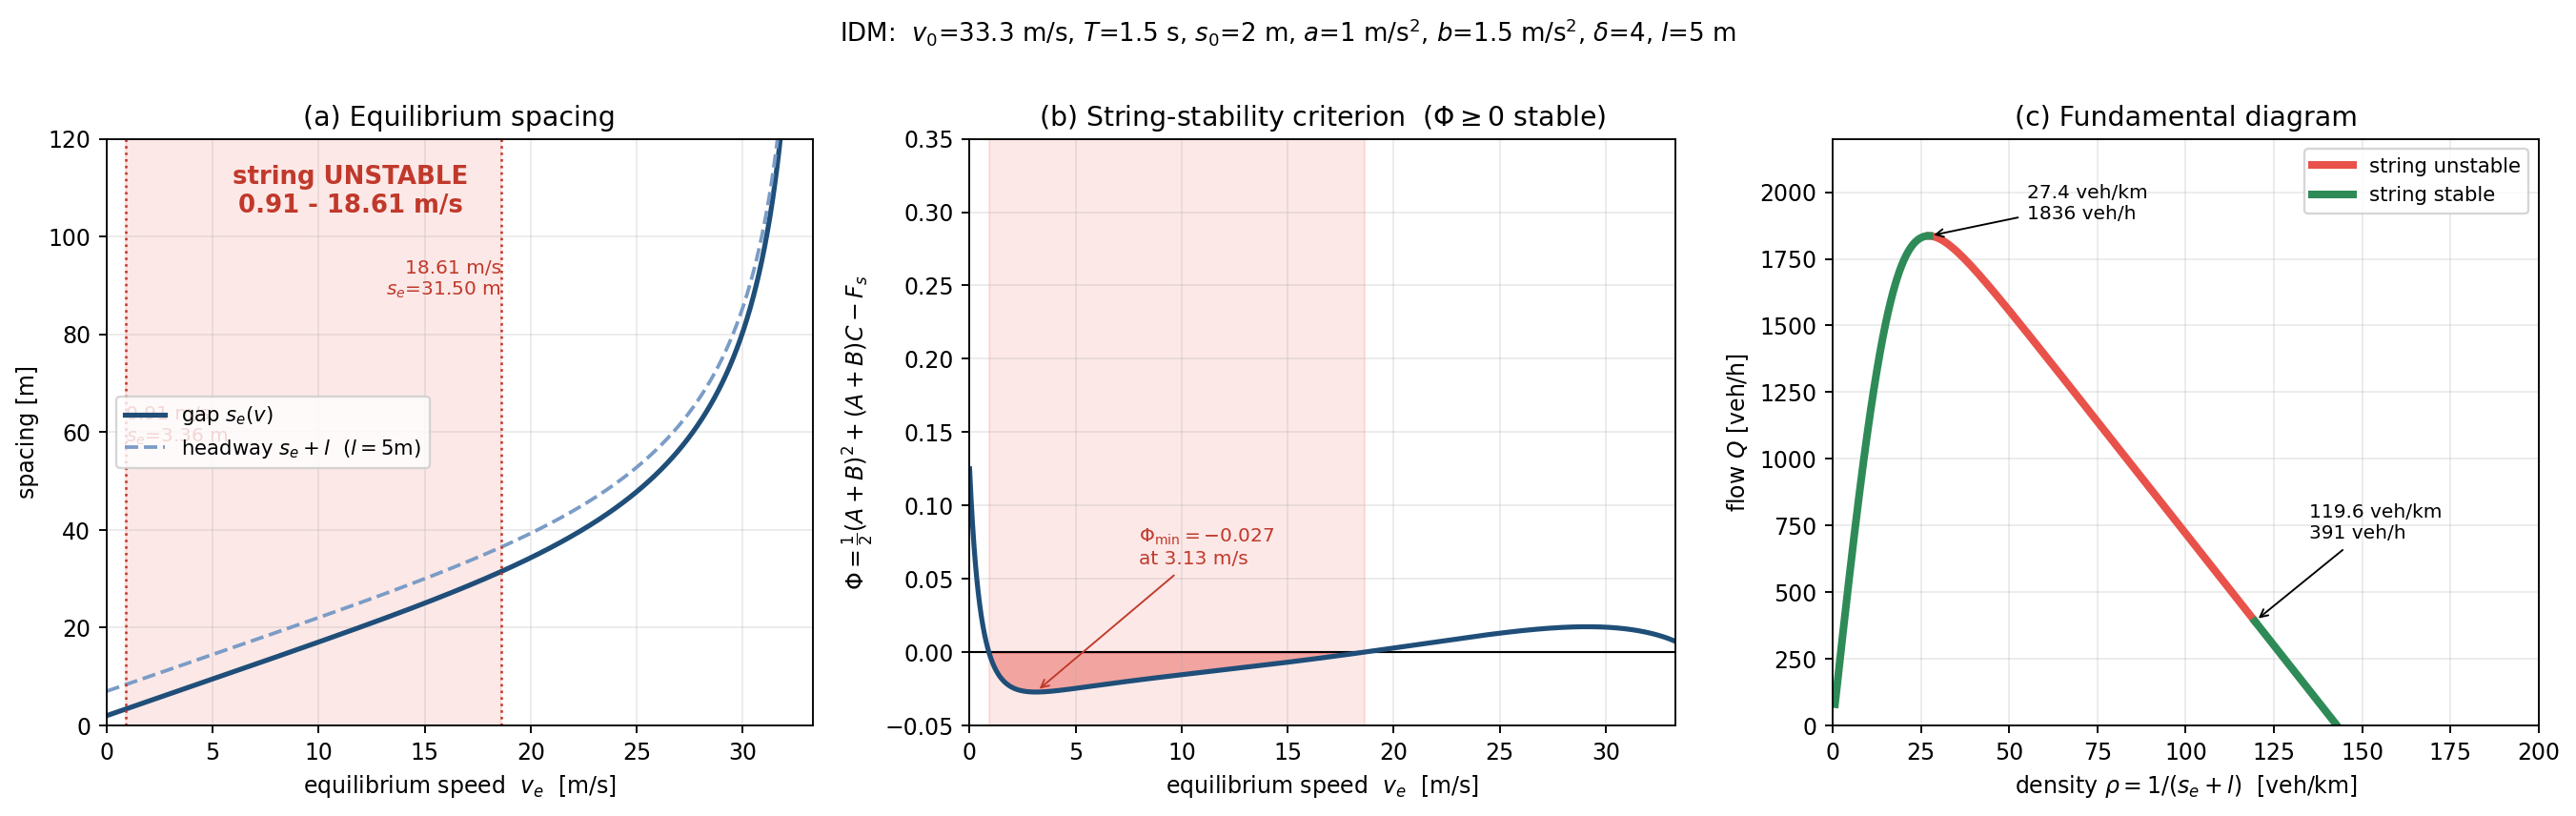
\includegraphics[width=\textwidth]{fig1.png}
\caption{原始 IDM 的平衡态、稳定判据与基本图。}
\label{fig:idm-stability-map}
\figurenote{基准 IDM 平衡分支与稳定域之间的一一映射。左图由 $F(s_e,v_e,0)=0$ 求出速度对应的平衡净间距，说明扫描 $v_e$ 的同时也在扫描密度；中图计算长波裕度 $\Phi(v_e)$，曲线穿越零线的两个交点给出失稳带上下边界，零线上方为稳定、下方为失稳。右图再利用 $\rho_e=1/(s_e+l)$ 和 $q_e=\rho_ev_e$ 把同一工作点投影到基本图，因此红色段不是经验涂色，而是中图负裕度区间在流量--密度坐标中的像。三图合读可以发现，流量相近的两个工作点可能位于不同稳定分支，说明仅知道基本图上的流量还不足以判断扰动会增长还是衰减。该图证明稳定性是一种附着在平衡分支上的动态属性；基本图规定“均匀态在哪里”，偏导和色散关系才规定“离开均匀态后往哪里走”。}
\end{figure}

几点值得注意：

\begin{itemize}[leftmargin=1.4em,itemsep=3pt]
\item \textbf{车长 $l$ 不进入稳定性判据。} 它只通过 $\rho = 1/(s_e+l)$ 影响基本图的横轴，因此图中不稳定段的密度与流量位置依赖 $l$，但临界速度 0.91 与 18.61 m/s 与 $l$ 无关。
\item \textbf{最容易失稳的是低速密集流}（$v_e\approx3$ m/s），而不是通行能力点。
\item 上临界点恰好落在基本图容量点（27.4 veh/km，1836 veh/h）右侧一点点，意味着这组参数下\textbf{通行能力附近就已经线不稳定}，扰动会向上游放大成走停波。这正是 IDM 常被用来复现 stop-and-go 现象的原因。
\item $v_e\to0$ 处 $\Phi\to 0.125>0$（因 $aT^2/s_0 = 1.125>1$），故完全停滞附近反而稳定，不稳定区间存在下边界。若将 $T$ 降到 $1.41$ s 以下，该下边界消失，不稳定区一直延伸到 $v_e=0$。
\item 全速域内局部稳定性始终满足；只是在不稳定带内 $f_v^2<4F_s$（欠阻尼），单车响应本身即为振荡衰减。
\end{itemize}

\section{数值验证 E1--E3：中性线、增长率与主导模态}
\sectionstudy{experiment}{数值验证 E1--E3：中性线、增长率与主导模态}{treiber2000,sugiyama2008,treiberkesting2013}
\label{sub:baseexp}

\begin{tcolorbox}[experimentbox,title=\textbf{实验设置}]
E1 在 $v_e\in(0,v_0)$ 上扫描 $\Phi(v_e)$ 并以二分法细化变号点。E2--E3 取 $N=120$、$v_e=8$ m/s、$s_e=14.0234$ m、$L=N(s_e+l)=2.2828$ km；在均匀平衡态上叠加幅值 $2\times10^{-3}$ m/s 的单一速度模态扰动。微观方程用四阶 Runge--Kutta 法、$\Delta t=0.02$ s 积分 300 s；在 $60$--$220$ s 的线性窗口拟合
\[
\operatorname{Re}\lambda=\frac{\mathrm d}{\mathrm dt}\ln|A_m(t)|,
\qquad
\operatorname{Im}\lambda=\frac{\mathrm d}{\mathrm dt}\arg A_m(t).
\]
空间 FFT 用于识别主导模态 $m^*$。所有拟合点均满足 $|A_m|<0.05$ m/s，以避免非线性饱和污染斜率。
\end{tcolorbox}

\begin{center}
\small
\captionof{table}{E1--E3 的解析预测与数值复现。}
\label{tab:e1e3-validation}
\begin{tabular}{p{2.0cm}p{3.6cm}p{3.6cm}p{3.2cm}}
\toprule
\textbf{实验} & \textbf{解析预测} & \textbf{数值结果} & \textbf{一致性} \\
\midrule
E1 中性线 & $0.91$--$18.61$ m/s & 扫描变号区间 $0.91$--$18.61$ m/s & 两个边界均复现 \\[3pt]
E2 增长率 & $\operatorname{Re}\lambda=0.00408566$ s$^{-1}$ & $0.00408565$ s$^{-1}$（321 点） & 相对误差 $3.7\times10^{-5}\%$ \\[3pt]
E2 频率 & $|\operatorname{Im}\lambda|=0.12821997$ rad/s & $0.12821997$ rad/s & 相对误差 $1.1\times10^{-6}\%$ \\[3pt]
E3 主导模态 & $m^*=4$，$k^*=0.20944$ rad/veh & FFT 峰值位于 $m=4$ & 完全一致 \\
\bottomrule
\end{tabular}
\end{center}
\tabletext{tab:e1e3-validation}{中性线、增长率、角频率和主导模态的解析值与微观仿真值。四项同时吻合说明验证不只是复现“稳定/失稳”标签，还定量复现了扰动的时间尺度与空间尺度。}

\begin{tcolorbox}[resultbox,title=\textbf{验证结论}]
解析增长率不仅给出“稳／不稳”的符号，而且定量预测了微观仿真中扰动包络的指数斜率与相位旋转速度。E3 同时验证：有限环道只能采样 $k_m=2\pi m/N$，因此仿真中出现的波长应与离散谱而非连续谱峰值比较。
\end{tcolorbox}

\section{具体轨迹结果：原始 IDM 的稳定与失稳}
\sectionstudy{experiment}{具体轨迹结果：原始 IDM 的稳定与失稳}{treiber2000,treiberkesting2013}

图~\ref{fig:traj-s0} 使用同一个局部减速脉冲，只改变平衡速度。稳定工况 $v_e=25$ m/s 中，$\sigma_v(1800)/\sigma_v(0)=0.00336$，探针车始终保持在 $24.9991$--$25.0006$ m/s、间距保持在 $54.8905$--$54.8996$ m；扰动色带很快消散。失稳工况 $v_e=8$ m/s 中，该比值增至 $48.49$，末段增长率为 $+3.12\times10^{-3}$ s$^{-1}$；探针车速度扩大到 $5.24$--$11.28$ m/s，间距扩大到 $9.73$--$19.67$ m。时空轨迹上的斜向红蓝带不断加深，直接显示扰动向上游传播并放大。

\begin{figure}[htbp]
\centering
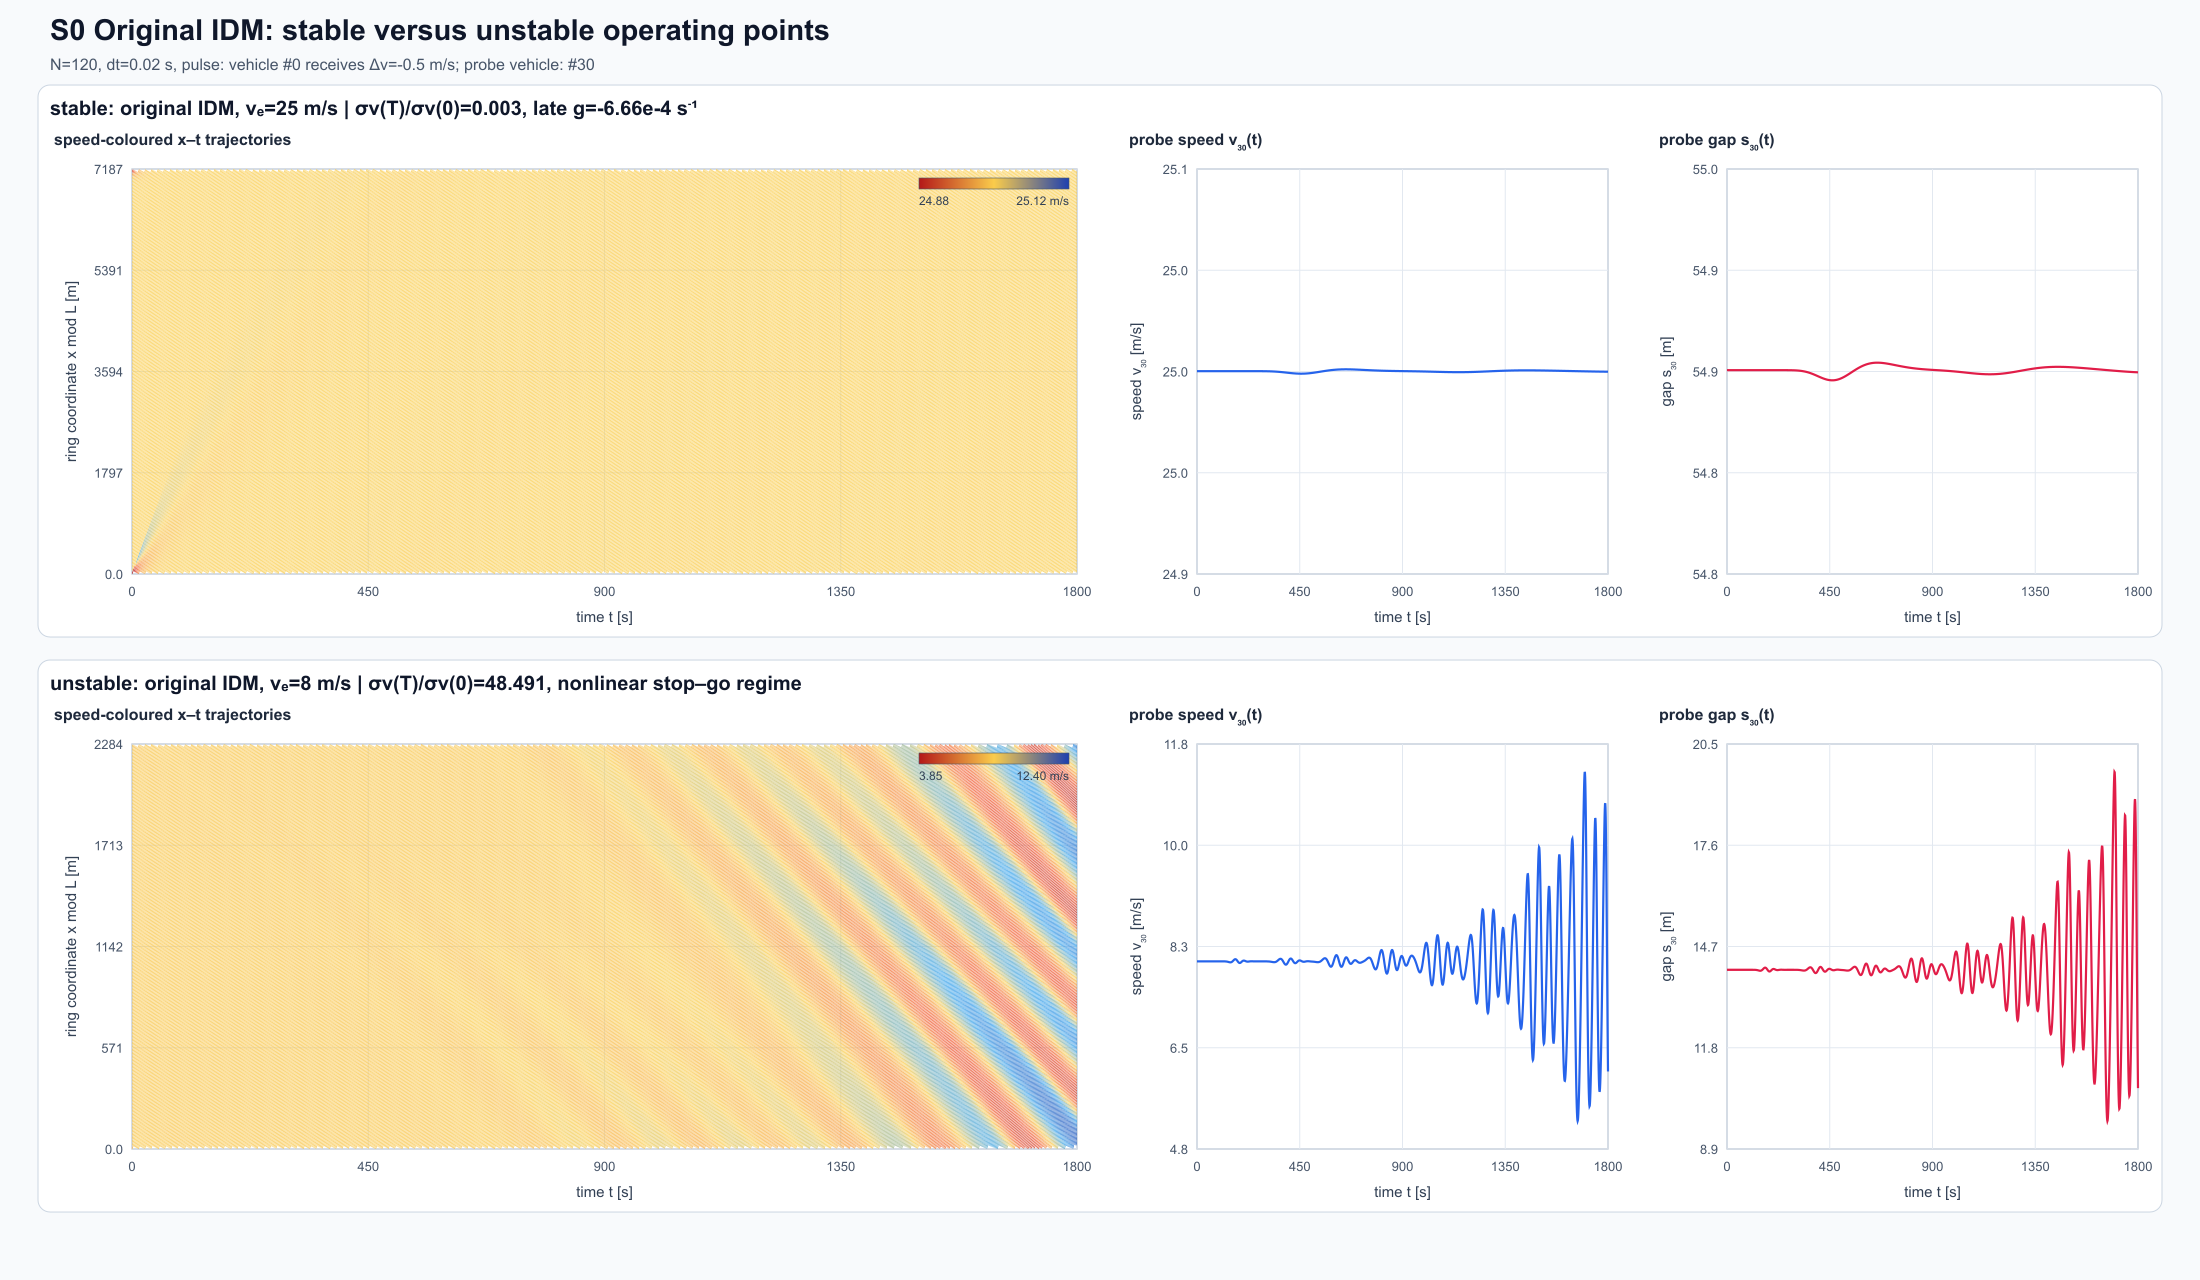
\includegraphics[width=\textwidth]{sim_s0_baseline.png}
\caption{S0：原始 IDM 的稳定与失稳轨迹。}
\label{fig:traj-s0}
\figurenote{S0 基准 IDM 在稳定和失稳工作点的完整时域对照。两行均取 $N=120$、$\Delta t=0.02$ s、1800 s 时间窗，并向第 0 辆车施加同一个 $-0.5$ m/s 速度脉冲；唯一关键差别是上、下行分别取 $v_e=25$ 和 $8$ m/s。左列是实际道路位置--时间轨迹，车辆轨迹的颜色表示瞬时速度：上行最初的低速色带在传播过程中逐渐变淡并恢复成近乎均匀的斜直线，说明扰动被吸收；下行的低速与高速色带逐圈加深、展宽并形成周期性走停波，说明小扰动已经进入非线性饱和。右侧指定第 30 辆车的速度和净间距曲线提供了局部证据：稳定工况的峰谷同步收敛，失稳工况的振幅持续增加且速度谷值对应间距压缩。两种图像对增长符号、传播方向和速度--间距耦合给出一致证据，因此该图不是单纯展示“堵或不堵”，而是直接验证 $\Phi(25)>0$ 与 $\Phi(8)<0$ 的解析判定。}
\end{figure}

\section{教学算例 M03：同一扰动下的原始 IDM 稳定／失稳对照}
\sectionstudy{experiment}{教学算例 M03：同一扰动下的原始 IDM 稳定／失稳对照}{treiber2000,treiberkesting2013}
\label{sec:mini-examples}

M03 是本章理论边界的最小动态核对。它比 1800 s 轨迹短，也只激发一个 Fourier
模态，因此可以直接比较解析增长率和拟合斜率；其余 M01、M02、M04--M06 已分别放在
局部稳定、长波、前车加速度、数值收敛和 LWR 章节。

取 $N=30$、$m=1$、初始速度模态幅值 $0.002$ m/s、$\Delta t=0.05$ s，积分 600 s。$v_e=25$ m/s 时，解析最右根为 $-0.0148584$ s$^{-1}$，仿真拟合为 $-0.0147203$ s$^{-1}$，末端幅值仅为初值的 $8.92\times10^{-5}$；$v_e=8$ m/s 时，解析值为 $+0.00408566$ s$^{-1}$，仿真拟合为 $+0.00408551$ s$^{-1}$，600 s 后幅值放大到初值的 $5.26$ 倍。两组只改变平衡速度，因而增长率符号与模态包络的差别可直接归因于稳定域。

\begin{figure}[htbp]
\centering
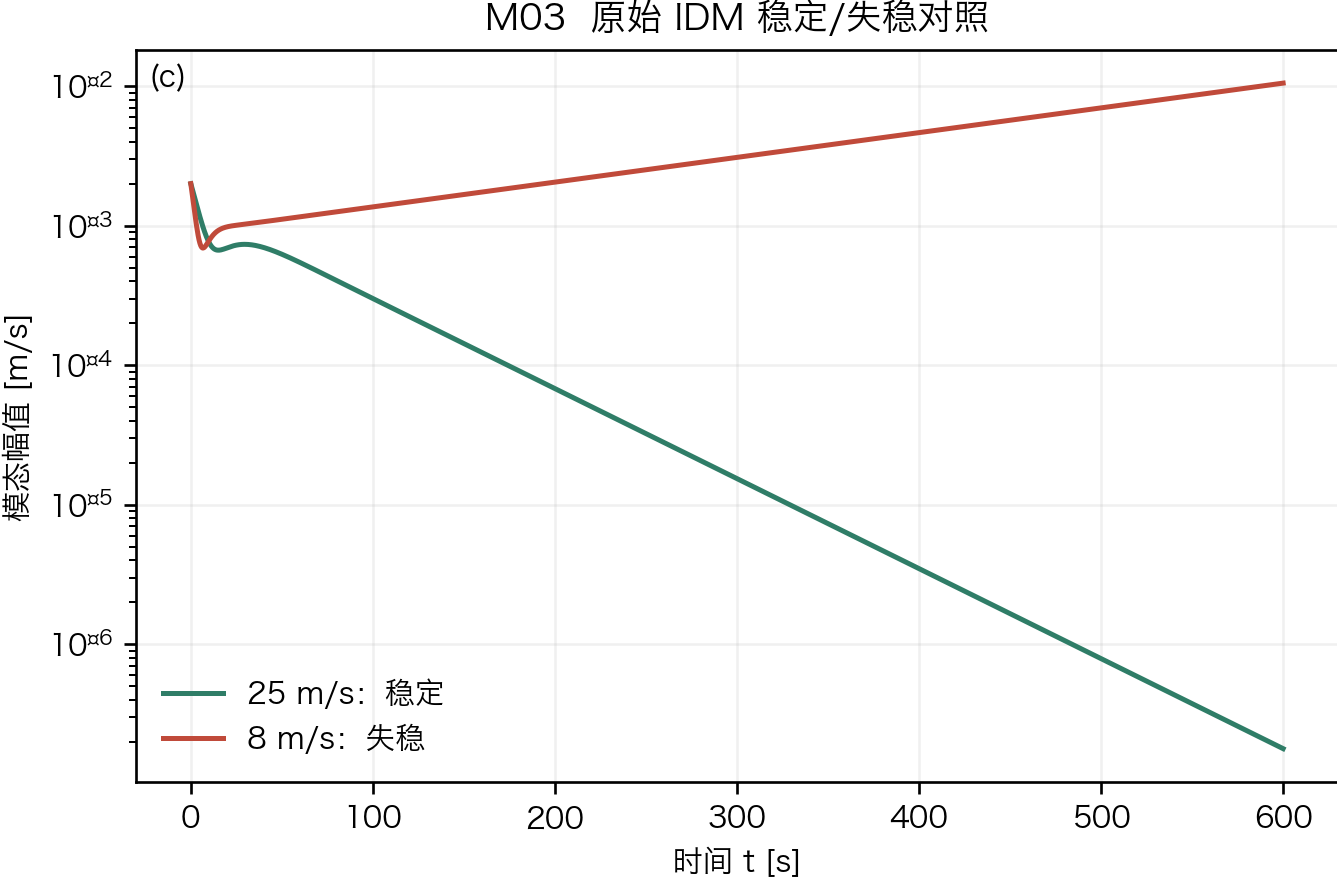
\includegraphics[width=0.86\textwidth]{mini_example_m03.png}
\caption{M03：原始 IDM 的模态包络。}
\label{fig:m03-baseline}
\figurenote{M03 从图~\ref{fig:traj-s0} 的完整非线性仿真中提取主导速度模态包络，并在对数纵轴上比较解析预测与拟合结果。在线性小扰动阶段，若 $A(t)\approx A_0e^{\sigma t}$，则 $\log A(t)$ 应为斜率 $\sigma$ 的直线；图中稳定工况向下倾斜、失稳工况向上倾斜，分别给出负、正增长率。拟合线与色散关系计算的 $\max_k\operatorname{Re}\lambda(k)$ 接近，说明位置--时间图中肉眼看到的色带变淡或加深不是色标造成的错觉，而是可量化的指数衰减或增长。后期失稳曲线偏离直线并趋于饱和，标志线性假设开始失效，而不是理论增长率计算错误。该图由此建立了解析谱、数值模态幅值和非线性时空图之间的证据链。}
\end{figure}

\begin{tcolorbox}[resultbox,title=\textbf{小算例与 1800 s 轨迹各回答什么}]
M03 用单一模态回答“解析增长率能否逐位复现”；图~\ref{fig:traj-s0} 的长算例回答“局部脉冲经过模态竞争后怎样形成真实走停波”。前者适合验算，后者适合观察完整演化，二者不能互相替代。
\end{tcolorbox}

%==================================================================
\sectionwrapup{基准算例用相同参数、相同扰动和 1800 s 时间窗验证解析结论：$v_e=25$ m/s 时位置--时间轨迹色差及指定车辆的速度／间距振荡衰减，$v_e=8$ m/s 时扰动增长为向上游传播的走停波。M03 的最小单模态实验又把理论／拟合增长率误差压到可直接核对的量级。}

\PART{II}{分析地图：从单因素到组合}

%==================================================================
\chapter{六个单因素速查}
\label{sec:map}
\chapterguide{加入新机制后，应该换哪一种稳定性工具}{本章不重复长推导，而是比较前馈、回望、多车、延迟和异质性分别破坏了哪一种结构。读者可据此判断应使用传递函数、环道谱、Bilharz 判据、延迟求根还是全系统本征值。}

在进入逐层推导之前，先把全部因素摊开。每个因素\textbf{单独}加到第~\ref{sec:num}~章的基准 IDM 上时的效果如下；组合情形见 \S\ref{sub:layers}。

\section{因素总表}
\sectionstudy{synthesis}{因素总表}{wilsonward2011,feng2019}

\begin{center}
\scriptsize
\captionof{table}{六个扩展因素对模型结构与判据的影响。}
\label{tab:six-factor-map}
\begin{tabular}{p{1.35cm}p{1.7cm}p{2.35cm}p{4.35cm}p{2.4cm}p{1.0cm}}
\toprule
\textbf{因素} & \textbf{记号} & \textbf{破坏的结构} & \textbf{单独作用时的判据} & \textbf{IDM 数字} & \textbf{详见} \\
\midrule
F1 前车加速度 & $f_a$ & 传函分子与分母同阶 & $\left|f_a\right|\le1$ 且 $\dfrac{f_v^2-f_{v_l}^2}{2}\ge\left(1-f_a\right)f_s$ & $\kappa_c=0.134$ & 第~\ref{sec:lead}~章 \\[8pt]
F2 后车加速度 & $f_b$ & \textbf{单向级联} & $\left|f_b\right|<1$、长波同上（$f_a\!\to\!f_b$），再加 $\widetilde W>0$ 的内部检验 & 正号窗口 $0.134$--$0.43$；负号单用有害 & 第~\ref{sec:bilat}~章 \\[12pt]
F3 多前／后车 & $\alpha,\beta$ & —（$P$ 变复杂） & 长波仅由 $\sigma_{\rm eff}=\dfrac{f_a}{1-\alpha}+\dfrac{f_b}{1-\beta}$ 决定 & $\alpha=0.8$ 时 $f_a=0.027$ 即可；$\beta\lesssim0.58$ & 第~\ref{sec:multi}~章 \\[12pt]
F4 后向间距 & $h_s,h_v$ & 单向级联，\textbf{且改变波速} & $c_1=\left(1-h_s/f_s\right)V'$；$\dfrac{2(f_s+\mu f_{v_l})}{\mu^2}\le\dfrac{1+p}{(1-p)^2}$ & $p_c=0.223$ & 第~\ref{sec:reargap}~章 \\[10pt]
F5 时间延迟 & $\tau_0,\tau_a$ & \textbf{多项式性} & 长波\textbf{完全不变}；新增 $\tau_0<\tau_0^{\rm crit}$ 与 $\Psi(\omega)\ge0$ & $\tau_0^{\rm crit}=1.16$--$2.52$ s & 第~\ref{sec:delay}~章 \\[8pt]
F6 车队异质 & $F_n\ne F_{n-1}$ & \textbf{平移不变性} & 前缀和 $\sum_{n\le j}\eta_n\ge0$，权重 $1/f_s^2$ & 环道总预算门槛 $26.7\%$ & 第~\ref{sec:het}~章 \\
\bottomrule
\end{tabular}
\end{center}
\tabletext{tab:six-factor-map}{前车/后车加速度、多车信息、后向间距、延迟和异质性分别破坏的数学结构。该表是后续章节的索引：先识别结构被破坏的位置，再选择传递函数、环道谱、Bilharz 或延迟数值方法。}

\section{六张结论卡片}
\sectionstudy{theory}{六张结论卡片}{wilsonward2011,feng2019}

\begin{tcolorbox}[keybox,title=\textbf{F1 前车加速度反馈（唯一"纯增益"因素）}]
唯一一个\textbf{既不破坏级联、也不改变波速}的因素。它只把长波条件的右端从 $f_s$ 降到 $(1-f_a)f_s$，代价是引入一条长波展开看不见的高频条件 $\left|f_a\right|\le1$（因为 $\left|G(i\infty)\right|=\left|f_a\right|$）。局部稳定性完全不受影响。
\end{tcolorbox}

\begin{tcolorbox}[keybox,title=\textbf{F2 后车加速度反馈（第一次破坏级联）}]
$y_n$ 开始依赖 $y_{n+1}$，"逐车放大倍数"这个概念本身失效，必须改用环形特征值 $+$ 复系数 Routh--Hurwitz。长波尺度上它与 F1 完全等价（只看总和），差别全在有限波长的相位项。\textbf{正号可用但窗口只有前视的三分之一；负号单独使用反而变差}（削减总量），必须配前视一起用。
\end{tcolorbox}

\begin{tcolorbox}[keybox,title=\textbf{F3 多车反馈（把增益摊薄）}]
指数衰减核可求和成闭式，$1/(1-\alpha)$ 恰是平均观测距离。长波门槛\textbf{仅由总量} $\sigma_{\rm eff}$ 决定，因此把同一总增益分配给多辆前车，可以按 $(1-\alpha)$ 降低最近邻增益。不过，空间分配仍具有\textbf{方向不对称性}：向前分配不降低长波裕度，向后分配则会增强一阶矩的不利贡献。
\end{tcolorbox}

\begin{tcolorbox}[keybox,title=\textbf{F4 后向间距反馈（唯一能改波速的因素）}]
与 F2 同样破坏级联，但作用在 $Q,R$ 而非 $P$，因此\textbf{能够直接降低运动学波速}，并在完全对称极限下使 $c_1\to0$。判据右端按 $(1-p)^{-2}$ 放宽，说明它兼具稳定裕度调节与波速调节能力；这与仅改变加速度核 $P$ 的反馈机制不同。\textbf{文献中的“后视效应”多数指这一类间距／相对速度反馈，而不是 F2 的后车加速度反馈。}
\end{tcolorbox}

\begin{tcolorbox}[keybox,title=\textbf{F5 时间延迟（只在有限频率上咬人）}]
特征方程变成拟多项式，有限维 Routh--Hurwitz 与 Bilharz 判据不再直接适用。但\textbf{长波条件保持不变}：当 $k\to0$ 时，$\lambda\to0$ 且 $e^{-\lambda\tau}\to1$。延迟的影响体现在两处：一是为局部稳定性引入反应时滞上限，二是可能使 $\Psi(\omega)$ 在有限频率处下降到零以下。
\end{tcolorbox}

\begin{tcolorbox}[keybox,title=\textbf{F6 车队异质（Fourier 失效，传函复活）}]
矩阵不再是循环矩阵，空间 Fourier 分析\textbf{根本不适用}；但单向级联仍在，逐车传递函数的\textbf{链式乘积}成为唯一好用的工具——与 F2／F4 正好相反。长波条件变成加权前缀和，权重 $1/f_s^2$ 使"迟钝"的车影响极大。
\end{tcolorbox}

\section{复杂度层级与工具选择}
\sectionstudy{synthesis}{复杂度层级与工具选择}{wilsonward2011,feng2019}
\label{sub:layers}

\begin{center}
\small
\captionof{table}{L0--L5 复杂度层级与可用分析工具。}
\label{tab:complexity-levels}
\begin{tabular}{p{1.0cm}p{4.0cm}p{3.4cm}p{4.8cm}}
\toprule
\textbf{层} & \textbf{包含的因素} & \textbf{特征方程类型} & \textbf{可用工具} \\
\midrule
L0 & 基准（单向、均匀、无延迟） & 二次，实结构 & 长波展开 $=$ 传递函数 \\[4pt]
L1 & $+$ F1、F3（仅前向） & 二次，复系数，级联保持 & \textbf{传递函数}（长波不够，须全频段） \\[4pt]
L2 & $+$ F2 或 F4 & 二次，复系数，级联断 & \textbf{环形特征值 $+$ Bilharz} \\[4pt]
L3 & $+$ F5 & \textbf{拟多项式} & 长波闭式 $+$ 全频段数值（D-分割／伪谱） \\[4pt]
L4 & $+$ F6 & 逐车不同 & \textbf{逐车传函链式乘积}；Fourier 失效 \\[4pt]
L5 & 组合（见下） & 视组合而定 & 两类简化可能同时失效 $\Rightarrow$ 直接求 $2N$ 维本征值 \\
\bottomrule
\end{tabular}
\end{center}
\tabletext{tab:complexity-levels}{从均匀单向无延迟到异质组合模型的复杂度阶梯。均匀性决定 Fourier 是否可用，单向性决定标量传递函数是否可用；二者同时丢失时必须求解完整状态矩阵。}

\begin{tcolorbox}[notebox,title=\textbf{一条判断规则}]
\[
\text{均匀性} \;\Longrightarrow\; \text{空间 Fourier 可用},
\qquad
\text{单向性} \;\Longrightarrow\; \text{传递函数可用}
\]
两者各失其一，就各失一种工具；两者同失（异质 $+$ 双向），只能直接做 $2N$ 维本征值。
\end{tcolorbox}

\section{本书处理的组合}
\sectionstudy{theory}{本书处理的组合}{wilsonward2011,feng2019}

\begin{center}
\small
\captionof{table}{本书重点处理的因素组合。}
\label{tab:factor-combinations}
\begin{tabular}{p{3.8cm}p{2.0cm}p{7.4cm}}
\toprule
\textbf{组合} & \textbf{层} & \textbf{新增的结论} \\
\midrule
F1 $+$ F2（双向） & L2 & 长波仅由 $\sigma=f_a+f_b$ 决定；不对称度从 $O(\varepsilon^3)$ 起作用，并控制有限波长分支（第~\ref{sec:bilat}~章） \\[6pt]
F3 双向（指数核） & L2 & 统一框架：任意核压缩进 $P(k)$；零阶矩管长波、一阶矩管有限波长（第~\ref{sec:multi}~章） \\[6pt]
F1 $+$ F5 & L3 & 长波门槛不动，只压增益上限；$\tau_a\approx\tau_0$ 时二者部分抵消（第~\ref{sec:delay}~章） \\[6pt]
F2 $+$ F5 & L3 & 标量传递函数与有限维 Bilharz 闭式均不再适用，需结合长波闭式与数值特征根 \\[6pt]
F6 $+$ F1（混合交通） & L4 & 前馈能力取决于\textbf{前车类型}，$\eta_n$ 依赖相邻对，连总和都依赖排序（\S\ref{sub:mixed}） \\
\bottomrule
\end{tabular}
\end{center}
\tabletext{tab:factor-combinations}{双向、多车、延迟和混合交通的代表性组合及新增结论。它说明组合模型并非简单叠加单因素结论，尤其异质性与双向耦合、前馈与通信延迟会改变可用的数学工具。}

%==================================================================
\sectionwrapup{六类因素可按是否改变单向级联、多项式结构和车辆均匀性分类。这个地图决定应使用传递函数、环道色散关系、复系数判据、延迟谱还是整车队矩阵，避免把不适用的闭式公式机械套用。}

\chapter{可复现数值实验协议}
\label{sec:protocol}
\chapterguide{怎样让“理论与仿真一致”成为可检查的结论}{本章固定初值、扰动、时间窗、数值步长、输出指标和收敛检查，并定义 E1--E14 的验证任务。它既是实验台的操作规范，也是全书所有图表可比较的前提。}

本章把后文分散出现的数值算例统一成一套可复现实验。配套实验台包含八个可叠加场景：S0 基准 IDM、S1 前车加速度、S2 后车加速度、S3 多前／后车、S4 后向间距、S5 时间延迟、S6 车型异质、S7 混合 AV/HDV。界面按“实时环道—传播与探针—理论与验证—模型设置”组织，使动画观察、参数控制和定量判断彼此分离。每个实验均同时报告\textbf{解析预测}与\textbf{仿真实测}，而不是仅凭动画判断稳定性。

\section{统一初值、扰动与数值格式}
\sectionstudy{numerical}{统一初值、扰动与数值格式}{sugiyama2008,treiberkesting2013}

除非实验另有说明，采用第~\ref{sec:num}~章 IDM 参数、$N=120$、$\Delta t=0.02$ s。给定密度或环长后先求公共平衡速度；均匀车流满足 $s_e=L/N-l$，异质车流则满足
\[
\sum_{n=1}^{N}\left[s_e^{(n)}(v_e)+l_n\right]=L,
\]
从而保证\textbf{同速不同距}的真正平衡态。默认扰动为单车速度脉冲或单一 Fourier 模态，幅值不超过 $2\times10^{-3}$--$5\times10^{-2}$ m/s。

\begin{tcolorbox}[experimentbox,title=\textbf{数值实现约定}]
\begin{enumerate}[leftmargin=1.6em,itemsep=3pt]
\item 无延迟基准使用四阶 Runge--Kutta；交互动画可使用半隐式更新，但定量表格须以 RK4 复核。
\item S2/S3 的加速度耦合写成 $(I-K)\bm a=\bm a_{\rm IDM}$。每一步求解循环带状线性系统，或固定点迭代至 $\|\bm a^{(r+1)}-\bm a^{(r)}\|_\infty<10^{-9}$；不得直接用上一步加速度替代。
\item S5 用环形历史缓冲区对 $t-\tau$ 作线性插值；历史段初始化为均匀平衡态。
\item 每个定量实验用 $\Delta t$ 与 $\Delta t/2$ 重跑。增长率、临界点或波速差异超过 $1\%$ 时，不接受该结果。
\item 报告拟合时间窗、样本数和扰动幅值；扰动进入非线性饱和后立即停止指数拟合。
\end{enumerate}
\end{tcolorbox}

\section{教学算例 M05：交通失稳与数值失稳怎样分开}
\sectionstudy{experiment}{教学算例 M05：交通失稳与数值失稳怎样分开}{sugiyama2008,treiberkesting2013}
\label{sub:m05-convergence}

对 M03 的失稳工况用 RK4 分别取 $\Delta t=0.4,0.2,0.1$ s，并把初始幅值
减至 $2\times10^{-4}$ m/s，在 $150$--$550$ s 拟合增长率。三次结果为
\[
0.0040856540,\qquad 0.0040856554,\qquad 0.0040856555\ {\rm s}^{-1},
\]
解析值是 $0.0040856555$ s$^{-1}$。对应相对误差依次为
$3.78\times10^{-5}\%$、$3.43\times10^{-6}\%$ 和
$1.53\times10^{-6}\%$。

\begin{figure}[htbp]
\centering
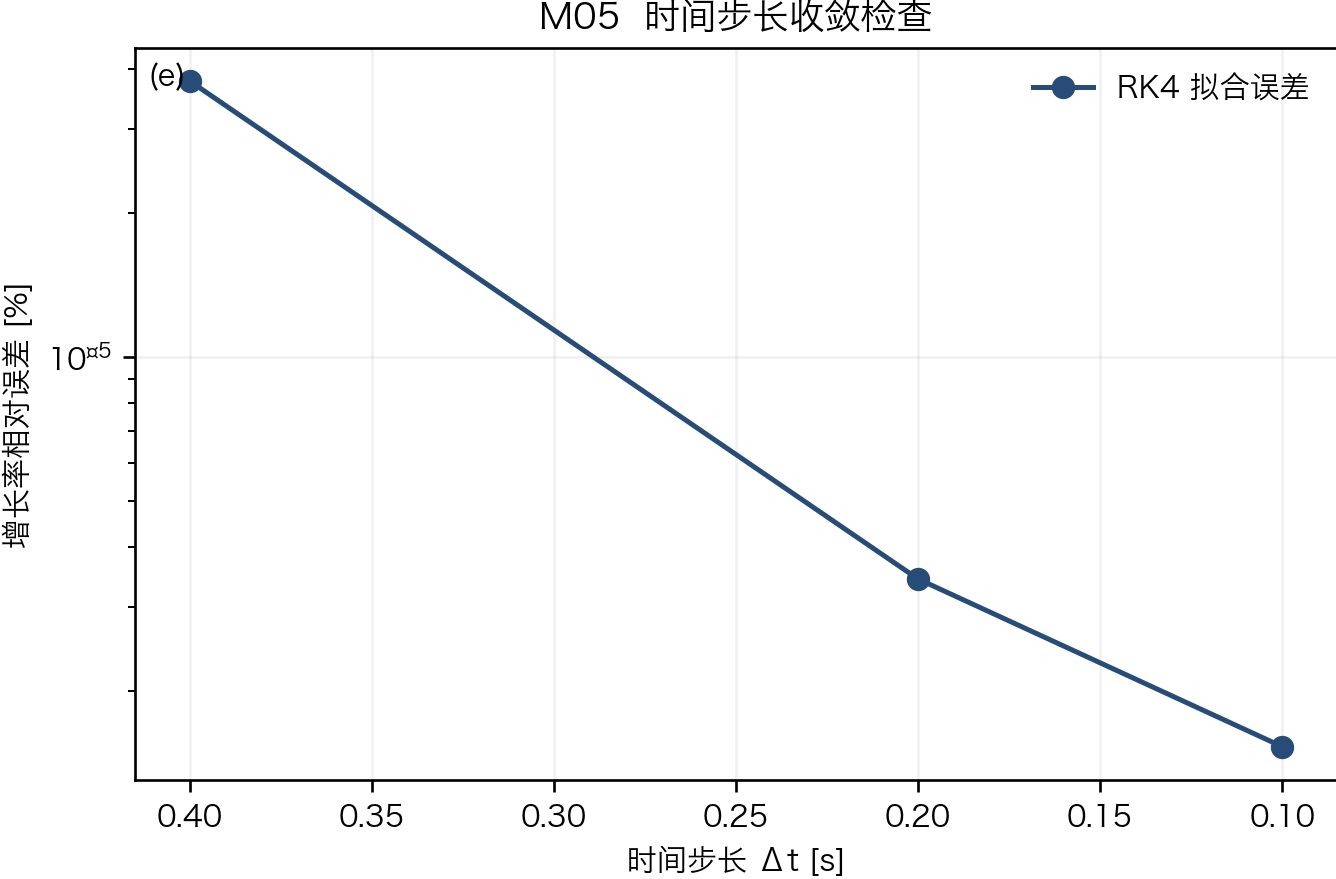
\includegraphics[width=0.82\textwidth]{mini_example_m05.png}
\caption{M05：时间步长收敛检查。}
\label{fig:m05-convergence}
\figurenote{M05 对时间离散误差进行的网格收敛检查。同一模型、初值、车辆数和拟合窗口只改变 RK4 步长，每个点重新计算主导增长率，并以最细步长或解析谱作为参照。随着 $\Delta t$ 减小，各点向稳定极限收敛，且 $\Delta t=0.02$ s 已落在变化很小的平台区，说明后续图中的增长符号和主要时间尺度不依赖某一个偶然步长。若粗步长点跨过零线，则会把数值阻尼误判为稳定或把离散振荡误判为失稳；本图明确排除了这种风险。它因此不是附带的程序测试，而是所有时域验证可信的前提，并给出了精度与 1800 s 长时计算成本之间的折中依据。}
\end{figure}

这里需要比较的是\textbf{同一个物理量的收敛}，而不是比较两张动画是否相似。
若减半步长后增长率变号、临界速度明显移动或出现负间距，则原结果不能用于验证稳定性。
反过来，M05 中正增长率在三个步长下保持到至少七位有效数字，说明增长来自 IDM
物理分支而非 RK4 离散误差。

\section{时空轨迹图与探针车曲线的统一画法}
\sectionstudy{experiment}{时空轨迹图与探针车曲线的统一画法}{sugiyama2008,treiber2000,treiberkesting2013}

除前述小扰动拟合实验外，后文还为 S0--S7 各给出一组\textbf{可直接观看扰动传播的长时域轨迹算例}。统一取 $N=120$、$\Delta t=0.02$ s、观测窗 $0\le t\le1800$ s；$t=0$ 时令第 0 辆车产生 $\Delta v_0=-0.5$ m/s 的局部减速脉冲，并固定观察第 30 辆车。

每组图的左列是真正的 $x$--$t$ \textbf{车辆时空轨迹}：纵轴为环道坐标 $x\bmod L$，每条细线是一辆车的轨迹，线色为该时刻的瞬时速度（红／橙表示较慢，蓝表示较快）。轨迹跨过 $x=L$ 时断开并从 $x=0$ 重新出现。右侧只画\textbf{一辆指定探针车}的 $v_{30}(t)$ 与 $s_{30}(t)$，而不是把全部车辆时序叠在一起。

图题中的 $\sigma_v(1800)/\sigma_v(0)$ 是全车速度标准差的首末比；线性阶段另报告末段包络斜率 $g=\mathrm d\ln\sigma_v/\mathrm dt$。若扰动已进入有限振幅走停波，则只把首末比与轨迹形态作为非线性结果，不再用末段 $g$ 解释线性增长率。

\section{在线干预实验：在同一条轨迹上比较控制前后}
\sectionstudy{experiment}{在线干预实验：在同一条轨迹上比较控制前后}{milanes2014,stern2018}

静态参数扫描回答“某组固定参数是否稳定”，但工程控制还需要回答另一个问题：\textbf{已经形成的走停波能否在不中断交通状态的情况下被逐步消除？} 为此，实验台允许仿真开始后改变前车加速度前馈增益、后车加速度增益、多车权重和后向间距权重；车辆的位置、速度、历史缓冲区和已记录图像均保留，不重新初始化。

为避免参数突变本身激发高频响应，前车加速度前馈采用线性渐变：若在 $t=t_{\rm int}$ 将增益由 $\kappa_-$ 调整到 $\kappa_+$，过渡时间为 $T_r$，则
\begin{equation}
\kappa(t)=
\begin{cases}
\kappa_-, & t<t_{\rm int},\\[2pt]
\kappa_-+(\kappa_+-\kappa_-)\dfrac{t-t_{\rm int}}{T_r},
& t_{\rm int}\le t<t_{\rm int}+T_r,\\[6pt]
\kappa_+, & t\ge t_{\rm int}+T_r.
\end{cases}
\label{eq:online-ramp}
\end{equation}
速度／间距时空图以标线记录 $t_{\rm int}$，因此同一幅图中可以直接比较干预前的波动增长、过渡阶段和干预后的衰减。

内置“拥堵形成 $\rightarrow$ 控制消散”算例取 $N=60$、$\rho=50$ veh/km、$\Delta t=0.02$ s，使用本书基准 IDM 参数，并令第 0 辆车产生 $-2.5$ m/s 的制动脉冲。系统先以原始 IDM（$\kappa=0$）演化，在 $t_{\rm int}=600$ s 将 $\kappa$ 用 $T_r=120$ s 平滑提高到 $0.45$。一次完整的平台复核中，速度标准差在 $t\approx543$ s 时达到 $0.534$ m/s，已形成可见走停波；干预后在 $t\approx974$ s 降至 $0.018$ m/s，环道重新接近均匀流。该算例说明控制器可以消散已经形成的非线性波动，但它\textbf{不替代} E1--E4 的小扰动临界增益与线性增长率测量。

\begin{tcolorbox}[experimentbox,title=\textbf{在线干预的判读顺序}]
先用环道动画确认拥堵波已经形成；再在速度与间距时空图上比较干预线两侧的色带宽度和传播方向；随后检查指定探针车的 $v_n(t)$、$s_n(t)$ 是否由周期性大幅振荡回到窄幅波动；最后用 $\sigma_v(t)$ 与 $\sigma_s(t)$ 的衰减确认改善不是局部或短时现象。若需估计稳定边界，仍应回到小幅 Fourier 扰动和固定参数实验。
\end{tcolorbox}

\section{测量量与判定规则}
\sectionstudy{theory}{测量量与判定规则}{sugiyama2008,treiberkesting2013}

\begin{center}
\small
\captionof{table}{稳定性实验的主要测量量与解析对应。}
\label{tab:experiment-observables}
\begin{tabular}{p{2.0cm}p{4.2cm}p{7.0cm}}
\toprule
\textbf{量} & \textbf{数值测法} & \textbf{与解析量的对应} \\
\midrule
增长率 & 对 $\ln|A_m(t)|$ 作最小二乘直线拟合 & 斜率与 $\max_m\operatorname{Re}\lambda_m$ 比较 \\[3pt]
主导波数 & 对 $v_n-\bar v$ 作空间 FFT & 峰值 $m$ 与 $\arg\max_m\operatorname{Re}\lambda_m$ 比较 \\[3pt]
波速 & 对主导模态相位展开后拟合 $\mathrm d\arg A_m/\mathrm dt$ & $c_1=-\operatorname{Im}\lambda/k$；时空图斜率只作辅助读数 \\[3pt]
传递比 & 开链中令头车作小幅正弦扰动，稳态后取幅值比 & 与 $|G(i\omega)|$ 或逐车乘积比较 \\[3pt]
中途峰值 & 沿车序计算 $\max_j|Y_j/Y_0|$ & 与 $\max_j\prod_{n\le j}|G_n|$ 比较 \\
\bottomrule
\end{tabular}
\end{center}
\tabletext{tab:experiment-observables}{增长率、主导波数、波速、逐车传递比和前缀峰值的数值测法。每个量都对应一个不同的解析对象，因此不能仅凭动画颜色判断稳定性。}

\section{E1--E14 与章节的对应}
\sectionstudy{experiment}{E1--E14 与章节的对应}{sugiyama2008,treiberkesting2013}

\begin{center}
\scriptsize
\captionof{table}{E1--E14 实验、操作与对应章节。}
\label{tab:experiment-index}
\begin{tabular}{p{0.85cm}p{2.3cm}p{3.5cm}p{4.2cm}p{2.7cm}}
\toprule
& \textbf{实验} & \textbf{操作} & \textbf{核心对照} & \textbf{对应章节} \\
\midrule
E1 & 中性稳定线 & 扫描 $v_e$ 或 IDM 参数并二分临界点 & 数值增长率变号 vs 判据函数变号 & 第~\ref{sec:num}~章 \\
E2 & 增长率 & 小扰动线性窗口拟合 & 实测 $\operatorname{Re}\lambda$ vs 环道谱 & \S\ref{sub:baseexp} \\
E3 & 最不稳定波数 & 空间 FFT & 实测 $m^*$ vs 谱峰 & 第~\ref{sec:bilat}~章, 第~\ref{sec:multi}~章 \\
E4 & 逐车传递比 & 开链正弦扫频 & $|Y_n/Y_{n-1}|$ vs $|G(i\omega)|$ & 第~\ref{sec:lead}~章 \\
E5 & 有限 $N$ & 扫描 $N=10$--$300$ & 临界带 vs $\cos(2\pi/N)$ & 第~\ref{sec:appx}~章 \\
E6 & 排序效应 & 固定配方，改变排列 & 中途峰值与末端乘积 & \S\ref{sub:hetorder} \\
E7 & AV 渗透率 & 扫描 AV 比例、速度与组数 & 二维稳定域、$p_{\min}$、$n_{\rm grp}^{\max}$ & \S\ref{sub:mixed} \\
E8 & 时间延迟 & 扫描 $\tau_0,\tau_a$ & $\Psi(0)$ 与 $\min_\omega\Psi$ & 第~\ref{sec:delay}~章 \\
E9 & 后视权重 & 扫描 $p$ & 不稳定带闭合点 $p_c$ & 第~\ref{sec:reargap}~章 \\
E10 & 波速 & 相位拟合与时空图 & $c_1=(1-p)V'(s_e)$ & 第~\ref{sec:reargap}~章 \\
E11 & 弱非线性演化 & 小幅正弦扰动长时积分 & 线性增长、波形陡化与饱和 & \S\ref{sub:nonlinear-exp} \\
E12 & 有限幅恢复 & 稳定工况扫描单车制动幅值 & 峰值、末窗残余与恢复时间 & 第~\ref{sec:nonlinear}~章 \\
E13 & 宏观稳定性 & IDM 基本图上的松弛 ARZ 稳定／失稳工作点 & 色散关系与定点速度--时间曲线 & \S\ref{sub:macro-experiment} \\
E14 & 微观--宏观一致性 & IDM 基本图与 ARZ 长波闭合下并排仿真 & 增长率、波速和速度时空图相似度 & \S\ref{sub:micro-macro-experiment} \\
\bottomrule
\end{tabular}
\end{center}
\tabletext{tab:experiment-index}{十四组实验的操作、理论对照与正文位置。读者可从实验编号反查对应推导，也可从章节选择相应的复现实验。}

\begin{tcolorbox}[notebox,title=\textbf{AV、HDV 与车型异质性是两套不同标签}]
S7 中 HDV 仅使用 IDM，前馈增益为 $0$；AV 跟随 AV 时使用 $\kappa$，跟随 HDV 时使用降级增益 $\kappa_0$。S6 则改变 $v_0,T,a,b$ 等车型／驾驶风格参数。两类标签可以叠加：一辆参数保守的车也可以装备自动驾驶控制器。除非明确启用 S6，AV 与 HDV 使用完全相同的 IDM 参数，因此 S7 的差异只来自信息与控制能力。
\end{tcolorbox}

\sectionwrapup{所有场景采用统一平衡初值、扰动幅值、1800 s 观测窗和收敛检查，并同时输出位置--时间速度着色轨迹、指定车辆速度／间距曲线及理论增长率。AV/HDV 标签表示控制能力，车型异质标签表示 IDM 参数差异，二者不可混用。}

\PART{III}{保持单向级联：前车加速度反馈}

\chapter{推广：考虑前车加速度效应}
\label{sec:lead}
\chapterguide{前车加速度前馈为什么能扩大稳定域}{本章说明纯前馈不改变单车局部根，却会改变车对车传递函数的分子和高频极限。读完后应能计算临界增益，并同时检查长波收益、有限频率峰值与增益上界。}

\section{模型设定}
\sectionstudy{model}{模型设定}{milanes2014,ploeg2014,feng2019}

在原有基础上加入前车加速度反馈（CACC 中的前馈项）：
\begin{equation}
\dot v_n = F\left(s_n,\; v_n,\; \dv_n,\; \dot v_{n-1}\right)
\end{equation}

仍换成等价形式 $\dot v_n = f(s_n,v_n,v_{n-1},\dot v_{n-1})$，平衡点处四个偏导：
\begin{equation}
f_s>0,\qquad f_v<0,\qquad f_{v_l}>0,\qquad
f_a \equiv \frac{\partial f}{\partial \dot v_{n-1}}\ \ (\text{一般}\ \ge 0)
\end{equation}

\textbf{平衡态不变.} 平衡时 $\dot v_{n-1}=0$，新增项自动为零，因此 $V(s_e)$ 与 $V'(s_e)$ 与前文完全相同。

线性化：
\begin{equation}
\delta\dot s_n = \delta v_{n-1}-\delta v_n,
\qquad
\delta\dot v_n = f_s\,\delta s_n + f_v\,\delta v_n + f_{v_l}\,\delta v_{n-1} + f_a\,\delta\dot v_{n-1}
\end{equation}

\section{局部稳定性：完全不变}
\sectionstudy{theory}{局部稳定性：完全不变}{wilsonward2011,ororsz2010}

前车匀速时 $\delta v_{n-1}\equiv 0$ 且 $\delta \dot v_{n-1}\equiv 0$，新增项\textbf{整项消失}，特征方程仍为
\begin{equation}
\lambda^2 - f_v\lambda + f_s = 0
\qquad\Longrightarrow\qquad
f_v<0,\quad f_s>0
\end{equation}

\begin{tcolorbox}[notebox]
前车加速度是纯前馈（feedforward），不进入自车闭环，对单车响应没有任何影响。这也说明：\textbf{单靠局部稳定性分析根本看不出加了这一项有什么好处}——它的作用只体现在车队层面。
\end{tcolorbox}

\section{线稳定性：传递函数}
\sectionstudy{theory}{线稳定性：传递函数}{swaroop1996,ploeg2014,feng2019}

用位置扰动：
\begin{equation}
\ddot y_n = f_s\left(y_{n-1}-y_n\right) + f_v\,\dot y_n + f_{v_l}\,\dot y_{n-1} + f_a\,\ddot y_{n-1}
\end{equation}

按 3.2 节完全相同的步骤，零初始条件下作 Laplace 变换（$\mathcal{L}\{\ddot y_{n-1}\}=\lambda^2Y_{n-1}$）：
\begin{equation}
\lambda^2 Y_n = f_s\left(Y_{n-1}-Y_n\right) + f_v\lambda Y_n + f_{v_l}\lambda Y_{n-1} + f_a\lambda^2 Y_{n-1}
\end{equation}

分离 $Y_n$ 与 $Y_{n-1}$：
\begin{equation}
\left(\lambda^2 - f_v\lambda + f_s\right)Y_n = \left(f_a\lambda^2 + f_{v_l}\lambda + f_s\right)Y_{n-1}
\end{equation}

\begin{tcolorbox}[keybox]
\begin{equation}
G(\lambda) = \frac{\hat y_n}{\hat y_{n-1}}
= \frac{f_a\lambda^2 + f_{v_l}\lambda + f_s}{\lambda^2 - f_v\lambda + f_s}
\label{eq:Ga}
\end{equation}
\end{tcolorbox}

与式~\eqref{eq:G0} 相比，关键变化是\textbf{分子多了 $\lambda^2$ 项}，于是
\begin{equation}
\lim_{\omega\to\infty}\left|G(i\omega)\right| = \left|f_a\right|
\end{equation}
不再趋于 0。这一点决定成败。

\section{条件的展开}
\sectionstudy{theory}{条件的展开}{milanes2014,ploeg2014,feng2019}
\label{sub:leadcond}

\begin{align}
\left|N(i\omega)\right|^2 &= \left(f_s - f_a\omega^2\right)^2 + f_{v_l}^2\omega^2 \\
\left|D(i\omega)\right|^2 &= \left(f_s - \omega^2\right)^2 + f_v^2\omega^2
\end{align}

利用平方差：
\begin{equation}
\left(f_s-\omega^2\right)^2 - \left(f_s-f_a\omega^2\right)^2
= \left(f_a-1\right)\omega^2\left[2f_s-\left(1+f_a\right)\omega^2\right]
\end{equation}

于是
\begin{equation}
\left|D\right|^2 - \left|N\right|^2
= \omega^2\Big\{\left(f_a-1\right)\left[2f_s-\left(1+f_a\right)\omega^2\right] + f_v^2 - f_{v_l}^2\Big\}
\end{equation}

令 $u = \omega^2 \ge 0$，花括号内整理为 $u$ 的\textbf{一次函数}：
\begin{tcolorbox}[keybox]
\begin{equation}
H(u) = \left(1-f_a^2\right)u + \left[f_v^2 - f_{v_l}^2 - 2f_s\left(1-f_a\right)\right] \;\ge\; 0
\qquad \forall\, u\ge 0
\end{equation}
\end{tcolorbox}

一次函数在 $[0,\infty)$ 上非负，当且仅当斜率非负且截距非负：

\begin{tcolorbox}[keybox,title=\textbf{一般线稳定性条件（含前车加速度）}]
\begin{align}
\text{(i)}\quad & \left|f_a\right| \le 1 \\[4pt]
\text{(ii)}\quad & \frac{1}{2}\left(f_v^2 - f_{v_l}^2\right) \;\ge\; \left(1-f_a\right)f_s
\end{align}
\end{tcolorbox}

$f_a=0$ 时即回到式~\eqref{eq:string}，自洽。用原始偏导写出（$f_a = F_{\dot v_l}$）：
\begin{equation}
\frac{1}{2}F_v^2 + F_vF_{\dv} \;\ge\; \left(1-f_a\right)F_s
\end{equation}

\section{长波展开为什么这次不够用}
\sectionstudy{theory}{长波展开为什么这次不够用}{milanes2014,ploeg2014,feng2019}

同样作 $\varepsilon=-ik\to0$ 展开，色散关系变为
\begin{equation}
\lambda^2\left(1-f_a e^{\varepsilon}\right) = f_s\left(e^{\varepsilon}-1\right) + \left(f_v+f_{v_l}e^{\varepsilon}\right)\lambda
\end{equation}

逐阶匹配得 $c_1 = V'(s_e)$ 不变，而
\begin{equation}
c_2 = \frac{\left(1-f_a\right)c_1^2 - \frac12 f_s - f_{v_l}c_1}{f_v+f_{v_l}}
\end{equation}

要求 $c_2\ge0$，整理后\textbf{恰好给出条件 (ii)，但给不出条件 (i)}。

\begin{tcolorbox}[notebox,title=\textbf{方法论要点}]
原因就在于 $\left|G(i\infty)\right| = \left|f_a\right|$：当 $f_a>1$ 时 $H(u)$ 斜率为负，失稳最先发生在 $\omega\to\infty$（短波），长波展开完全看不到。

\textbf{一旦模型含前车加速度，或出现任何使传递函数分子与分母同阶的项，就必须补做完整频域检验；单独使用长波展开可能遗漏高频失稳分支。}
\end{tcolorbox}

\section{物理解读}
\sectionstudy{theory}{物理解读}{milanes2014,ploeg2014,feng2019}

\textbf{条件 (i)：前馈增益不能过冲.} 前车加速度被放大后传给后车，高频段 $\left|G\right|\to f_a$。若 $f_a>1$，意味着每往后传一辆车、抖动就放大一次，整队在高频抖散。

\textbf{条件 (ii)：$f_a$ 起稳定作用.} 右端 $\left(1-f_a\right)f_s$ 随 $f_a$ 增大而减小，条件变宽松。极端情形 $f_a=1$（完美前馈）时条件变为
\begin{equation}
f_v^2 \ge f_{v_l}^2
\iff
\left|F_v+F_{\dv}\right| \ge \left|F_{\dv}\right|
\iff
-F_v \ge 0
\end{equation}
只要 $F_v<0$ 就\textbf{自动满足}，车队在任意平衡态都线稳定。这正是 V2V 通信（CACC）能大幅提升通行能力的理论依据。

\section{隐式形式的处理}
\sectionstudy{theory}{隐式形式的处理}{milanes2014,ploeg2014,feng2019}
\label{sub:implicit}

若模型写成相对加速度形式
\begin{equation}
\dot v_n = F\left(s,v,\dv\right) + \gamma\left(\dot v_{n-1}-\dot v_n\right)
\end{equation}

移项得
\begin{equation}
\dot v_n = \frac{F}{1+\gamma} + \frac{\gamma}{1+\gamma}\dot v_{n-1}
\qquad\Longrightarrow\qquad
f_a = \frac{\gamma}{1+\gamma} < 1 \quad (\gamma>0)
\end{equation}

同时 $f_s$、$f_v$、$f_{v_l}$ 全部按 $1/(1+\gamma)$ 缩放。这种写法\textbf{结构性地保证了条件 (i)}，代价是自车响应被整体钝化。代入条件 (ii)：
\begin{equation}
\frac{f_v^2-f_{v_l}^2}{2\left(1+\gamma\right)^2} \;\ge\; \frac{f_s}{\left(1+\gamma\right)^2}
\end{equation}

两边同乘 $\left(1+\gamma\right)^2$，缩放因子完全约掉：
\begin{equation}
\frac{1}{2}\left(f_v^2-f_{v_l}^2\right) \;\ge\; f_s
\end{equation}

\begin{tcolorbox}[notebox]
\textbf{相对加速度项对线稳定性完全无效}（缩放约掉了），只有真正的\textbf{绝对}前车加速度前馈才管用。
\end{tcolorbox}

\section{代回 IDM 算例}
\sectionstudy{experiment}{代回 IDM 算例}{treiber2000,treiberkesting2013}

取 $\dot v_n = F_{\mathrm{IDM}} + \kappa\,\dot v_{n-1}$（即 $f_a=\kappa$），判据变为
\begin{equation}
\Phi_\kappa(v_e) = \frac{1}{2}(A+B)^2 + (A+B)C - \left(1-\kappa\right)F_s \;\ge\; 0
\end{equation}

用第~\ref{sec:num}~章那组参数扫描全速域，要求所有 $v_e$ 均稳定所需的最小增益为

\begin{tcolorbox}[keybox]
\begin{equation}
\kappa_c = 0.134
\qquad
\left(\text{临界点出现在 } v_e\approx 8.88\ \text{m/s},\ s_e\approx15.4\ \text{m}\right)
\end{equation}
\end{tcolorbox}

也就是说，只要后车把\textbf{前车加速度的约 13.4\% 前馈}进自己的控制律，原来 0.91--18.61 m/s 那整段不稳定带就被彻底消掉。而这个 $\kappa$ 远小于稳定性上界 1，工程裕度很大。

\section{数值验证 E2/E4：前馈是否真的抑制放大}
\sectionstudy{experiment}{数值验证 E2/E4：前馈是否真的抑制放大}{milanes2014,ploeg2014,feng2019}

取与 E2 相同的 $N=120$、$v_e=8$ m/s 工况，把前馈增益设为 $\kappa=0.15>\kappa_c$。先对 $\omega\in[0,6]$ rad/s 扫描 $|G(i\omega)|$，再以微观仿真拟合最慢衰减模态。

\begin{center}
\small
\captionof{table}{E2/E4 前车加速度前馈的频域与时域验证。}
\label{tab:e2e4-front-feedforward}
\begin{tabular}{p{3.1cm}p{4.2cm}p{4.2cm}p{2.2cm}}
\toprule
\textbf{量} & \textbf{解析／频域预测} & \textbf{微观仿真实测} & \textbf{判定} \\
\midrule
逐车最大传递比 & $\max_\omega|G(i\omega)|=1$（$\omega=0$ 取等） & 正频率内未出现大于 1 的频带 & 不放大 \\[3pt]
最右增长率 & $-1.14052\times10^{-4}$ s$^{-1}$ & $-1.14051\times10^{-4}$ s$^{-1}$ & 衰减 \\[3pt]
主导离散模态 & $m^*=1$，$k=0.05236$ rad/veh & FFT 峰值 $m=1$ & 一致 \\
\bottomrule
\end{tabular}
\end{center}
\tabletext{tab:e2e4-front-feedforward}{逐车最大传递比、最右增长率和主导离散模态的预测与实测值。$\kappa=0.15$ 同时满足低频门槛和高频上界，并把基准工况的增长模态变为衰减模态。}

\begin{tcolorbox}[resultbox,title=\textbf{验证结论}]
$\kappa=0.15$ 只比全速域阈值高 $0.016$，但已经把 $v_e=8$ m/s 处的正增长率变成负值。实测与解析增长率的相对误差约 $6.5\times10^{-4}\%$。这同时验证了两个必要条件的分工：长波条件决定最低可用增益，而 $|\kappa|\le1$ 防止高频前馈过冲。
\end{tcolorbox}

\section{具体轨迹结果：前车加速度收益的稳定化作用}
\sectionstudy{application}{具体轨迹结果：前车加速度收益的稳定化作用}{ngsim2016,thiemann2008,krajewski2018}

图~\ref{fig:traj-s1} 固定 $v_e=8$ m/s 与同一扰动。无前馈时 $\sigma_v(1800)/\sigma_v(0)=48.49$；加入 $\kappa=0.15$ 后该比值降为 $0.0191$，末段斜率由 $+3.12\times10^{-3}$ 变为 $-3.89\times10^{-4}$ s$^{-1}$。第 30 辆车的速度范围由 $5.24$--$11.28$ m/s 收缩至 $7.994$--$8.009$ m/s，间距范围由 $9.73$--$19.67$ m 收缩至 $14.026$--$14.049$ m。

\begin{figure}[htbp]
\centering
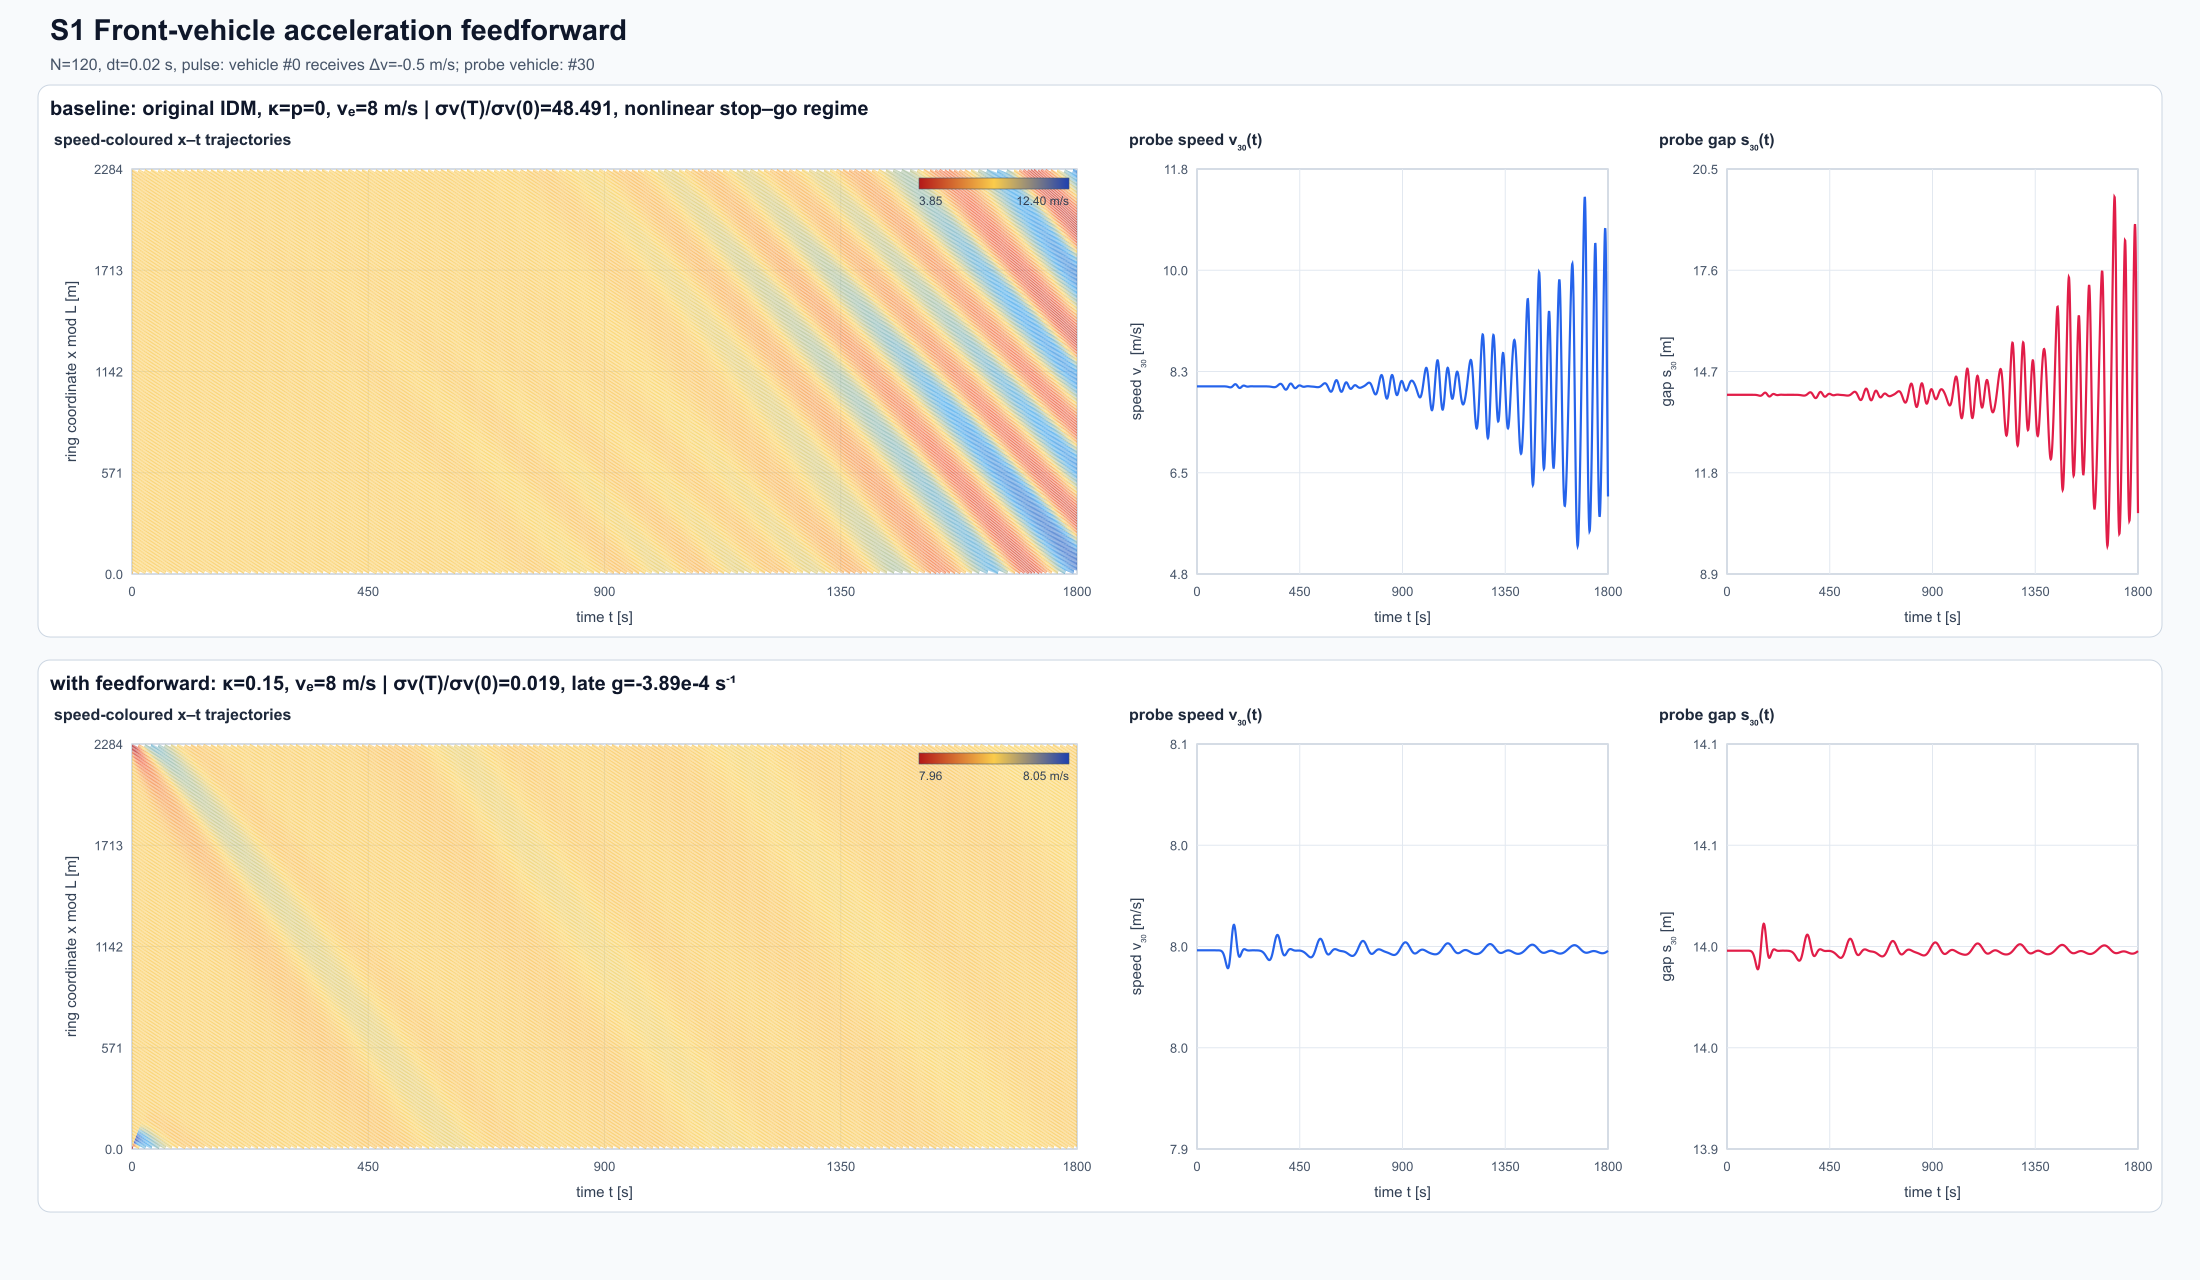
\includegraphics[width=\textwidth]{sim_s1_front_acc.png}
\caption{S1：前车加速度前馈的轨迹对照。}
\label{fig:traj-s1}
\figurenote{S1 前车加速度前馈对同一失稳车流的稳定化作用。上下两行复用图~\ref{fig:traj-s0} 的 $v_e=8$ m/s 工作点、车辆数、初始脉冲、色标和 1800 s 时间窗，只在下行加入 $\kappa=0.15$，因此构成受控的单因素比较。基准行的低速色带沿上游传播并在每次绕环后加深，探针速度和净间距的峰--峰值同步增加；加入前馈后，车辆提前获得前车加速度信息，色带在传播中逐渐变浅，两个探针量也回到平衡值。该图说明前馈并不是简单提高平均速度，而是改变扰动的空间传递增益，使同一个小脉冲由逐车放大转为逐车衰减。结合 $\kappa=0.15>\kappa_c=0.134$，时域恢复与解析阈值方向一致，从而证明临界增益具有可操作的控制含义。}
\end{figure}

\section{教学算例 M04：不重置状态，中途开启稳定控制}
\sectionstudy{experiment}{教学算例 M04：不重置状态，中途开启稳定控制}{milanes2014,ploeg2014,feng2019}
\label{sub:m04-online-control}

固定 $N=30$、$v_e=8$ m/s，把初始模态幅值提高到 $0.2$ m/s，使波动先在
原始 IDM 下发展。$t=300$ s 开始把前车加速度增益在 60 s 内由 0 线性提高到
$\kappa=0.25$；位置、速度和已经形成的波动全部保留，不重新初始化。
解析最右根由 $+0.00408566$ s$^{-1}$ 变为 $-0.0115580$ s$^{-1}$。
$240$--$300$ s 的平均速度标准差为 $0.19319$ m/s，而
$780$--$900$ s 降至 $8.08\times10^{-4}$ m/s，下降 $99.58\%$。

\begin{figure}[htbp]
\centering
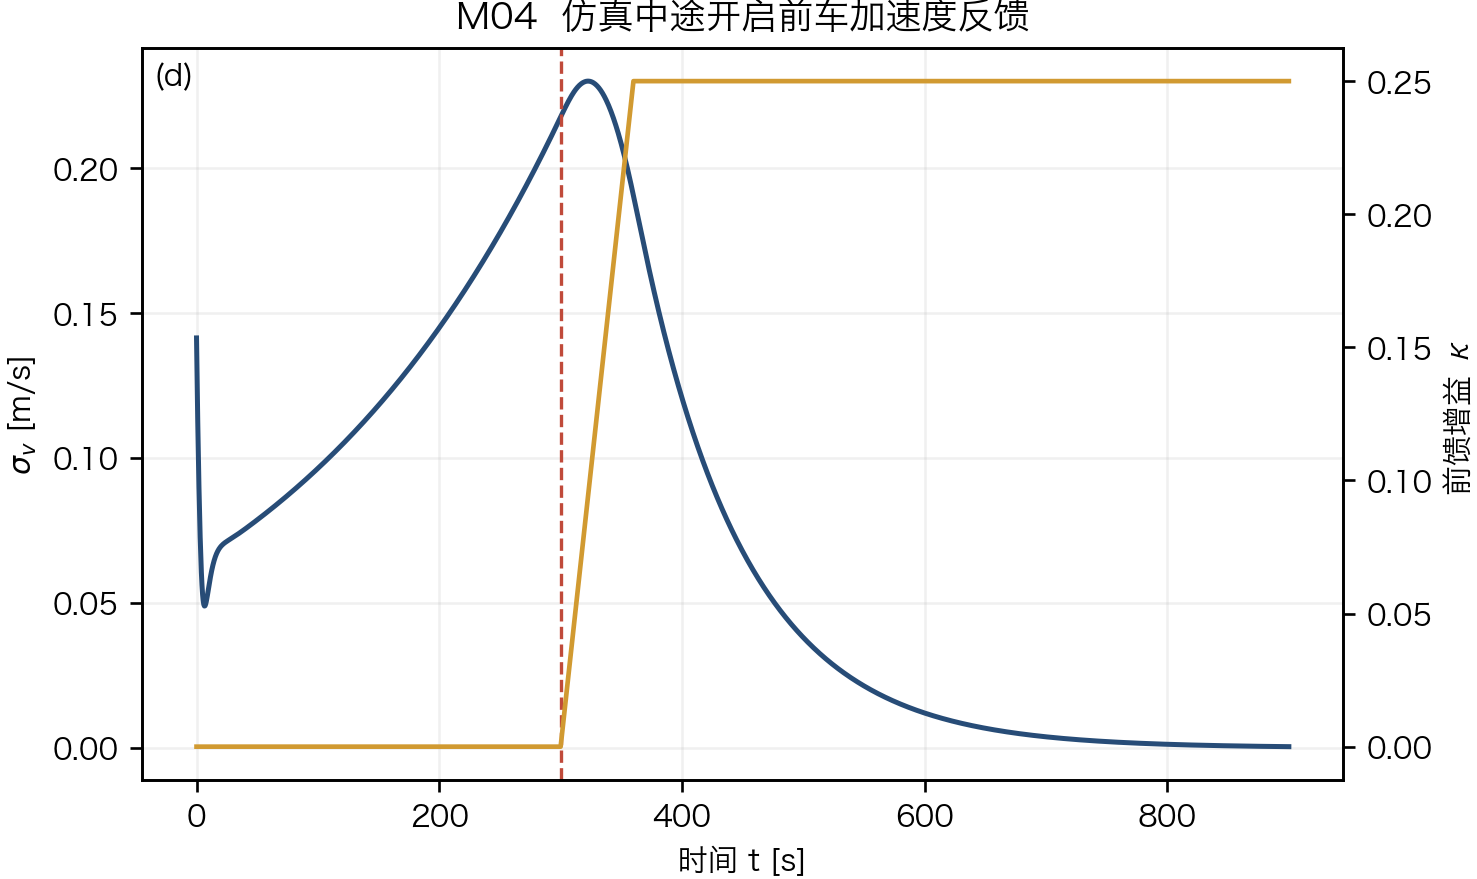
\includegraphics[width=0.88\textwidth]{mini_example_m04.png}
\caption{M04：运行中开启前车加速度反馈。}
\label{fig:m04-online-control}
\figurenote{M04 在线切换试验对“已经形成的走停波能否被消除”的回答。仿真开始时保持原始 IDM，使速度标准差先按失稳模态增长；红色虚线处不重置位置、速度或历史状态，只把黄色所示的前馈增益由零平滑切换到稳定区。切换前蓝色 $\sigma_v$ 的包络向上，切换后经过短暂过渡转为持续下降，证明控制改变的是当前系统的特征增长率，而不是依靠重新初始化制造一条平滑曲线。若只比较两个独立仿真，差异可能来自初值；本图的连续状态切换排除了这一混淆。它还揭示控制收益存在恢复时间：干预后扰动不会瞬间消失，而是以新的负增长率逐渐衰减，这对实际控制启停和持续时长设计十分重要。}
\end{figure}

静态对照只能说明“两个固定参数点不同”；M04 进一步说明参数切换后，
\textbf{已经存在的扰动}会从增长分支进入衰减分支。增益采用 60 s 渐变，
是为了避免不连续切换本身激发高频响应。

%==================================================================
\sectionwrapup{前车加速度前馈不改变单车局部恢复根，却能降低逐车传递幅值并扩大线稳定域。M04 又在不重置交通状态的条件下把速度标准差降低 $99.58\%$，展示已形成扰动的回稳过程；工程上仍必须联合检查有限频率峰值、通信延迟和执行器带宽。}

\PART{IV}{破坏单向级联：后车方向的耦合}

\chapter{再推广：同时考虑后车加速度（双向控制）}
\label{sec:bilat}
\chapterguide{双向耦合为何使标量级联失效}{本章从循环移位算子出发构造复系数色散关系，解释隐式加速度耦合为何必须整体求解，并用两条 Bilharz 条件分别检查总耦合与有限波长失稳。}

\section{先厘清"后车"的两种含义}
\sectionstudy{theory}{先厘清"后车"的两种含义}{swaroop1996,stuedli2017,feng2019}

\begin{itemize}[leftmargin=1.4em,itemsep=3pt]
\item 若"后车加速度"指\textbf{自车自身}的加速度 $\dot v_n$ 出现在右端，那是\textbf{隐式形式}，已在 \S\ref{sub:implicit} 处理：移项后化为等效的 $f_a$，并且结论是相对加速度项对线稳定性完全无效。
\item 若指\textbf{后方那辆车} $n+1$ 的加速度，则是\textbf{双向控制}（bilateral / look-back control）。这是本章的内容，也是结构上真正改变问题的情形。
\end{itemize}

\section{模型与线性化}
\sectionstudy{model}{模型与线性化}{swaroop1996,stuedli2017,feng2019}

\begin{equation}
\dot v_n = f\left(s_n,\; v_n,\; v_{n-1},\; \dot v_{n-1},\; \dot v_{n+1}\right)
\end{equation}

平衡点处新增两个偏导：
\begin{equation}
f_a \equiv \frac{\partial f}{\partial \dot v_{n-1}},
\qquad
f_b \equiv \frac{\partial f}{\partial \dot v_{n+1}}
\end{equation}

平衡态仍不变（平衡时两个加速度都为零）。线性化：
\begin{equation}
\ddot y_n = f_s\left(y_{n-1}-y_n\right) + f_v\dot y_n + f_{v_l}\dot y_{n-1}
+ f_a\ddot y_{n-1} + f_b\ddot y_{n+1}
\label{eq:bilin}
\end{equation}

\section{结构性变化：传递函数法失效}
\sectionstudy{theory}{结构性变化：传递函数法失效}{swaroop1996,ploeg2014,feng2019}
\label{sub:nofail}

\begin{tcolorbox}[notebox,title=\textbf{关键}]
$y_n$ 现在同时依赖 $y_{n-1}$ 和 $y_{n+1}$，车队\textbf{不再是单向级联}。第 $n$ 个方程无法解出与 $n$ 无关的 $Y_n/Y_{n-1}$——因为 $Y_{n+1}$ 又反过来依赖 $Y_n$。整个车队耦合成一个\textbf{三对角线性系统}，"逐车放大倍数"这个概念本身不再成立。

必须回到\textbf{空间 Fourier 分析／环形车队特征值分析}。
\end{tcolorbox}

\textbf{局部稳定性仍然不变.} 把前后两辆邻车都冻结为匀速，则 $\ddot y_{n\pm1}=0$，两个新增项同时消失，特征方程仍是 $\lambda^2-f_v\lambda+f_s=0$。

\section{为什么可以取 Fourier 模态：循环矩阵与 DFT}
\sectionstudy{proof}{为什么可以取 Fourier 模态：循环矩阵与 DFT}{swaroop1996,stuedli2017,feng2019}
\label{sub:circulant}

在写出模态解之前，先说明这不是"猜一个形式试试"，而是一次严格的本征分解。

\subsection{写成算子形式}

令 $\mathbf y=(y_1,\dots,y_N)^T$，定义\textbf{循环移位算子} $S$：
\begin{equation}
\left(S\mathbf y\right)_n = y_{n-1},
\qquad S^N = I \ \ (\text{周期边界})
\end{equation}

这里的“移位”是\textbf{车辆编号的移位}，不是车辆在道路上的实际位移；$y_n$ 才是第 $n$ 辆车相对平衡位置的位置扰动。$S$ 可以理解成一个“取前车数据”的操作：它把整列向量的每个分量都替换为对应前车的分量。

\begin{tcolorbox}[experimentbox,title=\textbf{用 4 辆车具体看懂移位算子}]
若环上有 4 辆车，记
\[
\mathbf y=
\begin{pmatrix}y_1\\y_2\\y_3\\y_4\end{pmatrix},
\qquad
S=
\begin{pmatrix}
0&0&0&1\\
1&0&0&0\\
0&1&0&0\\
0&0&1&0
\end{pmatrix}.
\]
则
\[
S\mathbf y=
\begin{pmatrix}y_4\\y_1\\y_2\\y_3\end{pmatrix},
\qquad
S^2\mathbf y=
\begin{pmatrix}y_3\\y_4\\y_1\\y_2\end{pmatrix},
\qquad
S^{-1}\mathbf y=
\begin{pmatrix}y_2\\y_3\\y_4\\y_1\end{pmatrix}.
\]
因此 $S$ 取第 $n-1$ 辆车（前车）的量，$S^{-1}$ 取第 $n+1$ 辆车（后车）的量，$I$ 保留本车的量。连续循环移位 4 次回到原向量，所以 $S^4=I$；一般 $N$ 辆车即有 $S^N=I$。
\end{tcolorbox}

基准模型的线性化方程就是
\begin{equation}
\ddot{\mathbf y} = \underbrace{f_s\left(S-I\right)}_{A}\mathbf y + \underbrace{\left(f_vI+f_{v_l}S\right)}_{B}\dot{\mathbf y}
\label{eq:shift-baseline}
\end{equation}
$A,B$ 都是 $S$ 的多项式，因而都是\textbf{循环矩阵}。这一步用到两个物理前提：\textbf{车队均匀}（每辆车规则相同）与\textbf{周期边界}（下标模 $N$）。

\subsection{把式~\eqref{eq:shift-baseline} 逐项拆回单车方程}

矩阵写法没有增加新的物理假设，只是一次写下全部 $N$ 辆车的方程。取式~\eqref{eq:shift-baseline} 的第 $n$ 个分量：
\begin{align}
\bigl[(S-I)\mathbf y\bigr]_n
&=(S\mathbf y)_n-(I\mathbf y)_n=y_{n-1}-y_n,\\
\bigl[(f_vI+f_{v_l}S)\dot{\mathbf y}\bigr]_n
&=f_v\dot y_n+f_{v_l}\dot y_{n-1}.
\end{align}
所以式~\eqref{eq:shift-baseline} 展开后恰好是
\begin{equation}
\ddot y_n=f_s(y_{n-1}-y_n)+f_v\dot y_n+f_{v_l}\dot y_{n-1},
\end{equation}
即每一辆车的基准线性化方程。下划括号只是给两个矩阵起名字：$A=f_s(S-I)$、$B=f_vI+f_{v_l}S$。

\begin{tcolorbox}[notebox,title=\textbf{为什么式~\eqref{eq:shift-baseline} 暂时没有写 $f_a$ 和 $f_b$}]
式~\eqref{eq:shift-baseline} 先用基准模型说明“循环移位”的结构，并没有漏掉双向加速度项。把式~\eqref{eq:bilin} 完整写成向量形式，应为
\begin{equation}
\left(I-f_aS-f_bS^{-1}\right)\ddot{\mathbf y}
=f_s(S-I)\mathbf y+\left(f_vI+f_{v_l}S\right)\dot{\mathbf y}.
\label{eq:bilin-shift}
\end{equation}
其中 $S\ddot{\mathbf y}$ 的第 $n$ 个分量是前车加速度 $\ddot y_{n-1}$，$S^{-1}\ddot{\mathbf y}$ 的第 $n$ 个分量是后车加速度 $\ddot y_{n+1}$。左边出现一个作用于全车加速度的循环矩阵，这正是每一步仿真必须联立求解、而不能再逐车级联计算的原因。
\end{tcolorbox}

\subsection{时间部分：常系数线性}

$A,B$ 是常数矩阵（平衡点处的偏导），系统线性时不变，解空间由 $e^{\lambda t}$ 张成。这是标准 ODE 结论，与车队结构无关。

\subsection{空间部分：循环矩阵被 DFT 基对角化}

$S$ 的本征向量正是离散 Fourier 基 $\left(\mathbf w_m\right)_n = e^{ikn}$：
\begin{equation}
\left(S\mathbf w_m\right)_n = e^{ik(n-1)} = e^{-ik}\left(\mathbf w_m\right)_n
\qquad\Longrightarrow\qquad
S\,\mathbf w_m = e^{-ik}\,\mathbf w_m
\end{equation}

\begin{tcolorbox}[notebox]
这顺带解释了前文所有 $e^{-ik}$ 的来历：\textbf{它就是移位算子的本征值}。多前车耦合中的 $P(k)=1-f_ae^{-ik}-f_be^{ik}$，无非是算子 $I-f_aS-f_bS^{-1}$ 的符号（symbol）。
\end{tcolorbox}

既然 $A,B$ 都是 $S$ 的多项式，它们与 $\mathbf w_m$ 同为本征向量、\textbf{被同一组基同时对角化}。$N$ 个耦合的二阶方程于是解耦成 $N$ 个独立的标量方程
\begin{equation}
\ddot{\hat y}_m = a(k)\hat y_m + b(k)\dot{\hat y}_m
\end{equation}
每个给出一个二次特征方程。所以"代入 $e^{\lambda t+ikn}$"是在\textbf{做本征分解}，不是试探解。

\subsection{$k$ 的量子化与完备性}

周期边界要求 $y_{n+N}=y_n$，即 $e^{ikN}=1$：
\begin{equation}
k = \frac{2\pi m}{N},\qquad m=0,1,\dots,N-1
\end{equation}
（$m$ 与 $m+N$ 给出同一模态，故只取 $N$ 个。）

\textbf{完备性：} 状态空间维数为 $2N$（$N$ 个位置 $+$ $N$ 个速度）；$N$ 个模态 $\times$ 每个二次方程 $2$ 个根 $=2N$，\textbf{恰好铺满}。所以"对所有 $m$ 检查 $\operatorname{Re}\lambda$"是充要的，不会漏根。

\subsection{两个技术性说明}

\begin{itemize}[leftmargin=1.4em,itemsep=4pt]
\item \textbf{$m=0$ 必须单独排除。} $\mathbf w_0=(1,\dots,1)^T$，而 $A\mathbf w_0=f_s(S-I)\mathbf w_0=0$（$A$ 只含差分，行和为零），特征方程退化为 $P\lambda^2-Q\lambda=0$，必有 $\lambda=0$。这个零根对应\textbf{整体平移}这一平凡对称性，永远中性。
\item \textbf{只需扫 $k\in(0,\pi]$。} 系数 $f_s,f_v,f_{v_l}$ 均为实数，故 $\lambda(-k)=\overline{\lambda(k)}$，$\operatorname{Re}\lambda$ 关于 $k$ 是偶函数，$k$ 与 $2\pi-k$ 给出相同增长率。
\end{itemize}

\begin{tcolorbox}[notebox,title=\textbf{什么时候这个假设失效}]
\begin{itemize}[leftmargin=1.2em,itemsep=2pt]
\item \textbf{车队不均匀}（$F_n\ne F_{n-1}$）$\Rightarrow$ 矩阵不再循环，DFT 基不再对角化——见 第~\ref{sec:het}~章；
\item \textbf{开链而非环道} $\Rightarrow$ 没有周期边界，$k$ 不量子化，正确的对象是传递函数（第~\ref{sec:appx}~章 证明 $N\to\infty$ 时二者等价）；
\item \textbf{有换道或异质扰动} $\Rightarrow$ 平移不变性被破坏。
\end{itemize}
\end{tcolorbox}

\section{环形车队的特征方程}
\sectionstudy{model}{环形车队的特征方程}{swaroop1996,stuedli2017,feng2019}

设 $N$ 辆车在环道上，取模态
\begin{equation}
y_n(t) = \hat y\,e^{\lambda t + ikn},
\qquad
k = \frac{2\pi m}{N},\quad m=0,1,\dots,N-1
\end{equation}

代入式~\eqref{eq:bilin}（注意 $y_{n\pm1}=y_n e^{\pm ik}$）并整理：
\begin{tcolorbox}[keybox]
\begin{equation}
P(k)\,\lambda^2 - Q(k)\,\lambda - R(k) = 0
\end{equation}
\begin{equation}
P(k) = 1 - f_a e^{-ik} - f_b e^{ik},
\qquad
Q(k) = f_v + f_{v_l}e^{-ik},
\qquad
R(k) = f_s\left(e^{-ik}-1\right)
\end{equation}
\end{tcolorbox}

稳定要求：对每个 $k\ne0$，两个根都在左半平面。$k=0$ 对应整体平移，永远是中性模态。

\section{复系数二次方程的判据（Bilharz 准则）}
\sectionstudy{proof}{复系数二次方程的判据（Bilharz 准则）}{swaroop1996,stuedli2017,feng2019}

由于 $P,Q,R$ 都是复数，不能直接用实系数 Routh--Hurwitz。化为首一形式
\begin{equation}
\lambda^2 + c_1\lambda + c_0 = 0,
\qquad
c_1 = -\frac{Q}{P} = p_1 + iq_1,
\qquad
c_0 = -\frac{R}{P} = p_2 + iq_2
\end{equation}

\begin{tcolorbox}[keybox,title=\textbf{二次复系数多项式的稳定判据}]
两根均满足 $\operatorname{Re}\lambda<0$ 当且仅当
\begin{equation}
p_1 > 0
\qquad\text{且}\qquad
\Delta_2 \equiv p_1\left(p_1p_2 + q_1q_2\right) - q_2^2 > 0
\end{equation}
\end{tcolorbox}

判据的完整证明见附录~\ref{sec:theorem-reference}：先由韦达定理把 $p_j,q_j$ 写成两根实部与虚部的组合，再证明
\begin{equation}
\Delta_2 = \alpha_1\alpha_2\left[\left(\alpha_1+\alpha_2\right)^2 + \left(\beta_1-\beta_2\right)^2\right].
\end{equation}
因此 $p_1>0$ 与 $\Delta_2>0$ 恰好排除任一根进入闭右半平面。这里不能直接套用实系数 Routh--Hurwitz，因为 $c_1,c_0$ 一般不是实数。

\section{化简：两个实多项式条件}
\sectionstudy{theory}{化简：两个实多项式条件}{swaroop1996,stuedli2017,feng2019}
\label{sub:twocond}

令
\begin{equation}
u = \cos k \in [-1,\,1),
\qquad
\sigma = f_a+f_b \ \ (\text{总耦合强度}),
\qquad
d = f_a-f_b \ \ (\text{不对称度})
\end{equation}

下面先把“经代数化简”拆成一条可追踪的路线；所有乘法与系数收集见附录~\ref{sec:bilharz-algebra}。记
\begin{equation}
s_k=\sin k,
\qquad
D(u)=|P(k)|^2=(1-\sigma u)^2+d^2(1-u^2).
\label{eq:D-bilateral}
\end{equation}
在 $P(k)\ne0$（即 $D>0$）的正则情形，乘以共轭 $\overline P$ 后可把四个实系数写成
\begin{align}
p_1&=\frac{\Pi(u)}{D(u)},
&q_1&=\frac{s_k\,\Xi(u)}{D(u)},\\
p_2&=\frac{f_s(1-u)\,\Gamma(u)}{D(u)},
&q_2&=\frac{f_ss_k\,\Omega(u)}{D(u)},
\label{eq:pq-bilateral}
\end{align}
其中
\begin{align}
\Pi(u)&=-\left(f_v+f_{v_l}u\right)+\sigma f_vu+f_{v_l}\left(d+2f_bu^2\right),\\
\Xi(u)&=d\left(f_v+f_{v_l}u\right)+f_{v_l}(1-\sigma u),\\
\Gamma(u)&=1+d-2f_bu,
&\Omega(u)&=1-d-2f_bu.
\label{eq:aux-bilateral}
\end{align}

第一条 Bilharz 条件立即变成
\begin{equation}
p_1>0
\iff
\frac{\Pi(u)}{D(u)}>0
\iff
\Pi(u)>0,
\end{equation}
因为 $D(u)>0$。第二条看似更复杂，但代入式~\eqref{eq:pq-bilateral} 后所有高次项恰好因式分解为
\begin{equation}
\Delta_2
=p_1(p_1p_2+q_1q_2)-q_2^2
=\frac{f_s(1-u)}{D(u)^2}\,\widetilde W(u).
\label{eq:Delta-factor}
\end{equation}
对非平凡模态 $k\ne0$，有 $f_s>0$、$1-u>0$、$D^2>0$，所以 $\Delta_2$ 的符号只由 $\widetilde W$ 决定。于是两个条件化为：

\begin{tcolorbox}[keybox,title=\textbf{条件 I}]
\begin{equation}
\Pi(u) \equiv -\left(f_v + f_{v_l}u\right) + \sigma f_v u + f_{v_l}\left(d + 2f_b u^2\right) \;>\; 0
\label{eq:Pi-bilateral}
\end{equation}
\end{tcolorbox}

\begin{tcolorbox}[keybox,title=\textbf{条件 II}]
\begin{equation}
\widetilde W(u) = w_3u^3 + w_2u^2 + w_1u + w_0 \;>\; 0
\label{eq:Wpoly-bilateral}
\end{equation}
\begin{align}
w_3 &= -4f_b^2 f_s \\
w_2 &= 2f_b\left[2f_s\left(1-f_a\right) + f_{v_l}\left(f_{v_l}-f_v\right)\right] \\
w_1 &= -f_s\left(1-\sigma\right)^2 + 4f_b^2f_s - \sigma f_v^2 + \left(1+\sigma\right)f_vf_{v_l} - f_{v_l}^2 \\
w_0 &= -f_s\left(1-d\right)^2 + f_v^2 - f_vf_{v_l} + d\,f_{v_l}\left(f_{v_l}-f_v\right)
\label{eq:Wcoeff-bilateral}
\end{align}
\end{tcolorbox}

两个端点值特别简洁：
\begin{align}
\widetilde W(1) &= \left(1-\sigma\right)\left[f_v^2 - f_{v_l}^2 - 2f_s\left(1-\sigma\right)\right]
\label{eq:W1}\\
\widetilde W(-1) &= \left(1+\sigma\right)\left(f_v-f_{v_l}\right)^2
\end{align}
\begin{equation}
\Pi(1) = \left(\sigma-1\right)\left(f_v+f_{v_l}\right)
\end{equation}

\section{三条闭式结论}
\sectionstudy{theory}{三条闭式结论}{swaroop1996,stuedli2017,feng2019}

\begin{tcolorbox}[keybox,title=\textbf{(A) 总耦合强度上界}]
由 $\Pi(1)>0$ 且 $f_v+f_{v_l}<0$：
\begin{equation}
\sigma = f_a + f_b \;<\; 1
\end{equation}
再由 $\widetilde W(-1)>0$ 得 $\sigma>-1$。故\textbf{必要条件 $\left|f_a+f_b\right|<1$}。
\end{tcolorbox}

\begin{tcolorbox}[keybox,title=\textbf{(B) 长波条件：只依赖 $f_a+f_b$}]
由式~\eqref{eq:W1} 及 $\sigma<1$：
\begin{equation}
\frac{1}{2}\left(f_v^2 - f_{v_l}^2\right) \;\ge\; \left(1-f_a-f_b\right)f_s
\end{equation}
\textbf{前视与回望的加速度反馈在长波尺度上完全等价，只有总和 $\sigma$ 起作用。}（可由长波展开独立验证：$c_1=V'(s_e)$ 不变，$c_2$ 的表达式中 $f_a$ 恰好被 $\sigma$ 替代，而不对称度 $d$ 要到 $O(\varepsilon^3)$ 才出现。）
\end{tcolorbox}

\begin{tcolorbox}[keybox,title=\textbf{(C) 有限波长条件：不对称性在此起作用}]
$\widetilde W$ 是 $u$ 的\textbf{三次}多项式，最高次系数 $w_3=-4f_b^2f_s\le0$。当 $f_b\ne0$ 时曲线可以在区间内部下穿零点，此时端点检验\textbf{不再充分}，必须扫描 $u\in[-1,1)$。
\end{tcolorbox}

\section{三个特例}
\sectionstudy{theory}{三个特例}{swaroop1996,stuedli2017,feng2019}
\label{sub:special}

\textbf{(1) $f_b=0$（纯前视，即第~\ref{sec:lead}~章）.} 此时 $w_3=w_2=0$，$\widetilde W$ 退化为\textbf{线性}函数，最小值必在端点取得，条件即
\begin{equation}
\left|f_a\right| \le 1
\qquad\text{且}\qquad
\frac{1}{2}\left(f_v^2-f_{v_l}^2\right) \ge \left(1-f_a\right)f_s
\end{equation}
——与 \S\ref{sub:leadcond} 用传递函数得到的结果\textbf{完全一致}。这同时交叉验证了两套方法。

\textbf{(2) $f_b=f_a$（对称双向）.} 此时 $P = 1-2f_a\cos k$ 为\textbf{实数}，$d=0$，$\widetilde W$ 可因式分解：
\begin{equation}
\widetilde W(u) = \left(1-2f_au\right)B(u),
\qquad
B(u) = 2f_af_su^2 + \left[2f_af_s - f_s + f_vf_{v_l} - f_{v_l}^2\right]u + \left[f_v^2-f_vf_{v_l}-f_s\right]
\end{equation}
其中 $1-2f_au>0$ 对一切 $u$ 成立 $\iff \left|f_a\right|<\tfrac12 \iff \sigma<1$，与结论 (A) 一致。剩下只需 $B(u)>0$。

\textbf{(3) $f_a=0$（纯回望）.} $\widetilde W$ 是完整的三次式，$w_3<0$。数值上会看到：增益较小时可以稳定，但\textbf{增益增大到某个中等值后反而失稳}——纯回望的加速度耦合在短波段会自激。

\section{数值算例}
\sectionstudy{experiment}{数值算例}{swaroop1996,stuedli2017,feng2019}
\label{sub:multinum}

仍取第~\ref{sec:num}~章的 IDM 参数，在 $v_e=8$ m/s（基准模型此处线不稳定）计算：
\[
f_s = 0.1421,\qquad f_v = -0.6803,\qquad f_{v_l} = 0.4650
\]
长波阈值为
\[
\sigma \;\ge\; 1 - \frac{f_v^2-f_{v_l}^2}{2f_s} = 0.133
\]

\begin{figure}[htbp]
\centering
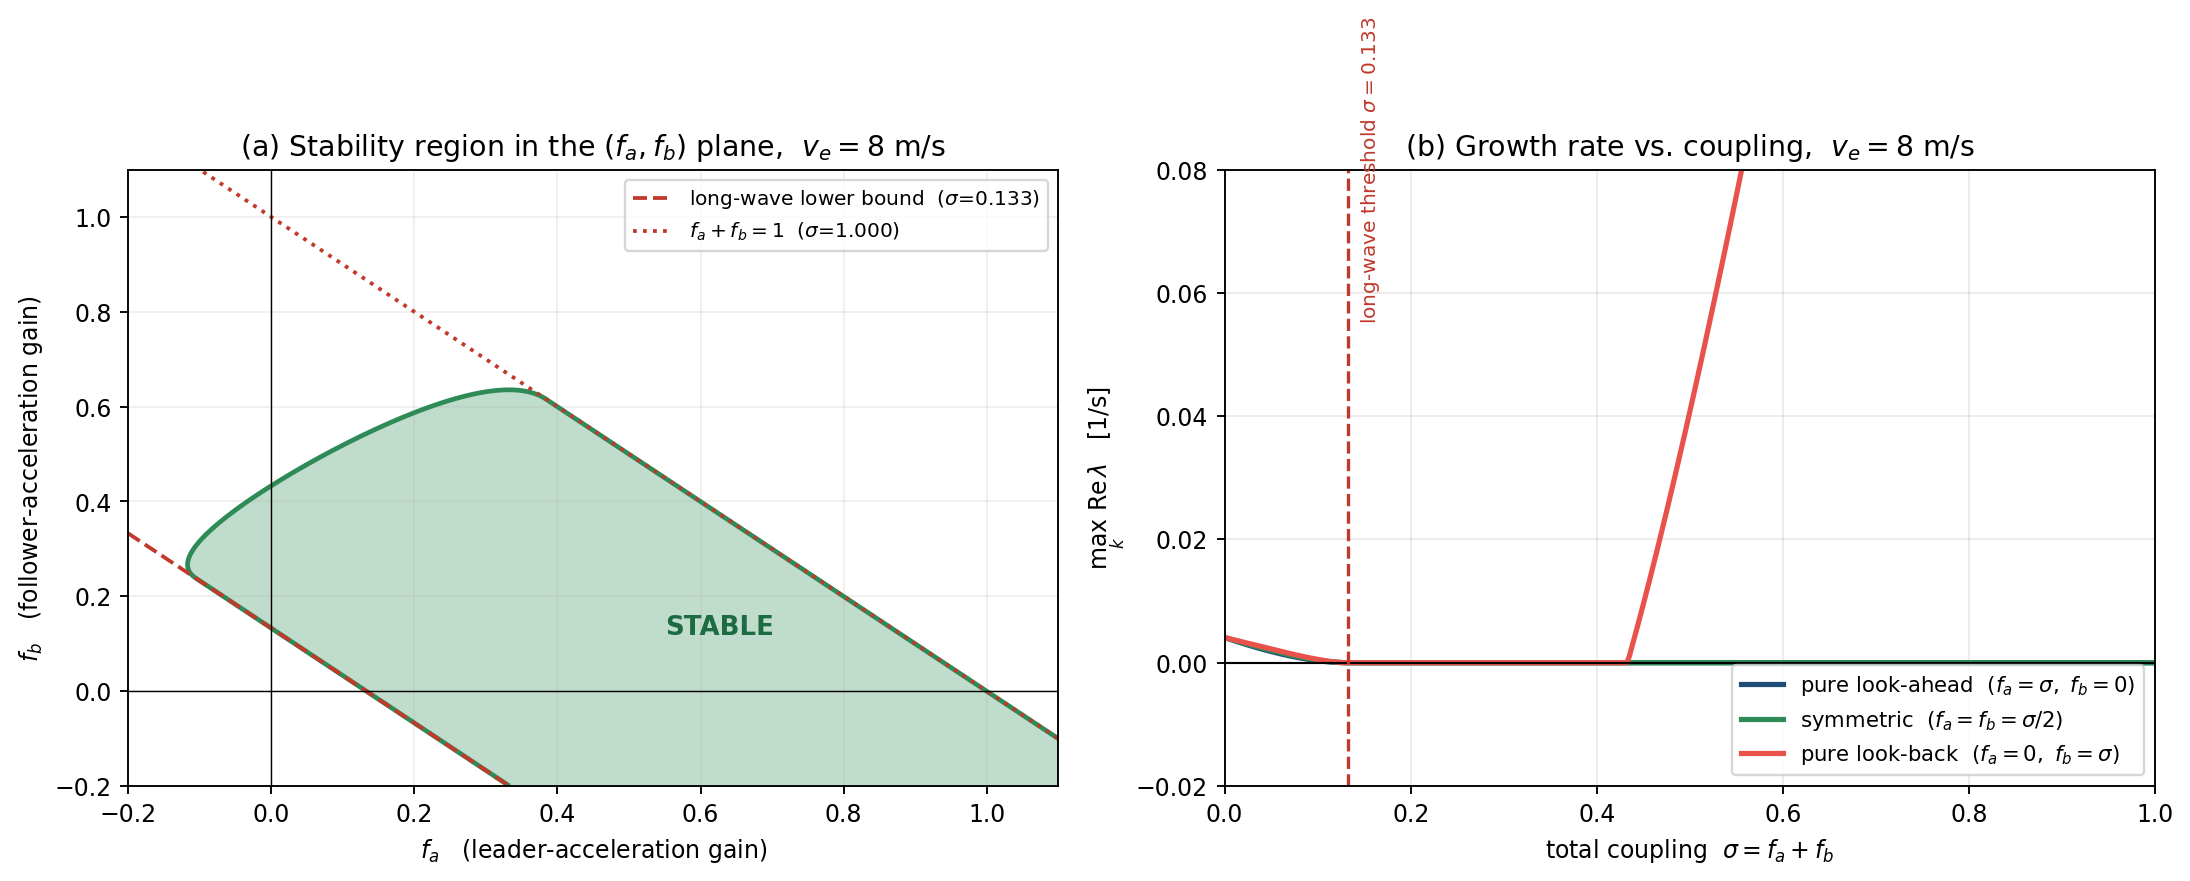
\includegraphics[width=\textwidth]{fig2.png}
\caption{双向加速度耦合的稳定域与增长率。}
\label{fig:bilateral-domain}
\figurenote{双向加速度耦合的完整稳定域以及“总量相同并不等于全谱相同”。左图在 $(f_a,f_b)$ 平面逐点扫描所有离散波数，稳定区的直线下边界由 $f_a+f_b$ 的长波门槛决定，而弯曲上边界来自某个有限 $k$ 模态首先穿越虚轴；因此只检查 $k\to0$ 会错误地把弯曲边界之外的点判成稳定。右图把横坐标改为总耦合 $\sigma=f_a+f_b$，并比较纯前视、混合和纯回望三种分配；三条曲线在约 $0.133$ 处同时穿过零线，实证零阶总量控制长波起点。继续增大 $\sigma$ 后，前视方案仍改善，而纯回望在约 $0.43$ 处重新出现正增长率，揭示回望方向的一阶矩会侵蚀有限波长裕度。该图证明控制设计必须分两步：先用总量越过长波门槛，再用全波数扫描排除分配引起的二次失稳。}
\end{figure}

\begin{tcolorbox}[notebox,title=\textbf{工程结论}]
\begin{itemize}[leftmargin=1.2em,itemsep=3pt]
\item 要消除走停波，关键是\textbf{加速度反馈的总量} $f_a+f_b$ 达到阈值，前视或回望都可以贡献。
\item 但\textbf{回望不能单独承担太多}：$f_b$ 过大会在短波段引入新的失稳分支。稳定域在 $f_b$ 方向明显比 $f_a$ 方向窄。
\item 总耦合必须满足 $f_a+f_b<1$，这是硬上界。
\item 综合看，\textbf{前视为主、回望为辅}的配置（稳定域中 $f_a$ 大、$f_b$ 适中的那片区域）裕度最大。这与 CACC 实践中以前车信息为主的设计相符。
\end{itemize}
\end{tcolorbox}

\section{数值验证 E3：双向隐式耦合}
\sectionstudy{experiment}{数值验证 E3：双向隐式耦合}{swaroop1996,stuedli2017,feng2019}

取 $N=120$、$v_e=8$ m/s，比较基准模型与“前视为主、回望为辅”的 $(f_a,f_b)=(0.30,0.10)$。每个 RK4 子步均求解循环线性系统 $(I-f_aS-f_bS^{-1})\bm a=\bm a_{\rm IDM}$，残差阈值取 $10^{-9}$。

\begin{center}
\small
\captionof{table}{E3 双向隐式耦合的主导模态与增长率。}
\label{tab:e3-bilateral}
\begin{tabular}{p{3.4cm}p{3.2cm}p{3.4cm}p{3.2cm}}
\toprule
\textbf{场景} & \textbf{$m^*$} & \textbf{$\max\operatorname{Re}\lambda$ [s$^{-1}$]} & \textbf{结果} \\
\midrule
S0 基准 IDM & 4 & $+0.00408566$ & 扰动增长 \\
S2：$f_a=0.30,f_b=0.10$ & 1 & $-0.00148012$ & 扰动衰减 \\
\bottomrule
\end{tabular}
\end{center}
\tabletext{tab:e3-bilateral}{基准 IDM 与双向耦合工况的主导模态和最右根。总反馈量为 0.40 后，增长率由正变负，验证了循环隐式求解与 Fourier 特征值的一致性。}

参数扫描还给出纯正回望的全速域窗口约 $0.134\le f_b\le0.43$：下边界来自长波总量，弯曲上边界来自有限波长。因而实验报告必须同时给出 $m^*$ 与最右根，不能只验证 $f_a+f_b$ 是否超过长波阈值。

\begin{tcolorbox}[resultbox,title=\textbf{验证结论}]
加入总量 $f_a+f_b=0.40$ 的双向加速度反馈后，最右根从 $+4.09\times10^{-3}$ 移到 $-1.48\times10^{-3}$ s$^{-1}$。循环隐式求解与 Fourier 特征值给出相同稳定符号；若用“上一步加速度”显式替代，临界附近会引入额外相位误差，不作为定量证据。
\end{tcolorbox}

\section{具体轨迹结果：双向加速度耦合}
\sectionstudy{experiment}{具体轨迹结果：双向加速度耦合}{ngsim2016,thiemann2008,krajewski2018}

图~\ref{fig:traj-s2} 在同一 $v_e=8$ m/s 失稳点加入 $(f_a,f_b)=(0.30,0.10)$。全车扰动首末比由基准的 $48.49$ 降至 $0.00106$，末段斜率为 $-1.48\times10^{-3}$ s$^{-1}$，与本章最右特征根一致。第 30 辆车的速度仅在 $7.9981$--$8.0017$ m/s 内变化，间距仅在 $14.0326$--$14.0381$ m 内变化。

\begin{figure}[htbp]
\centering
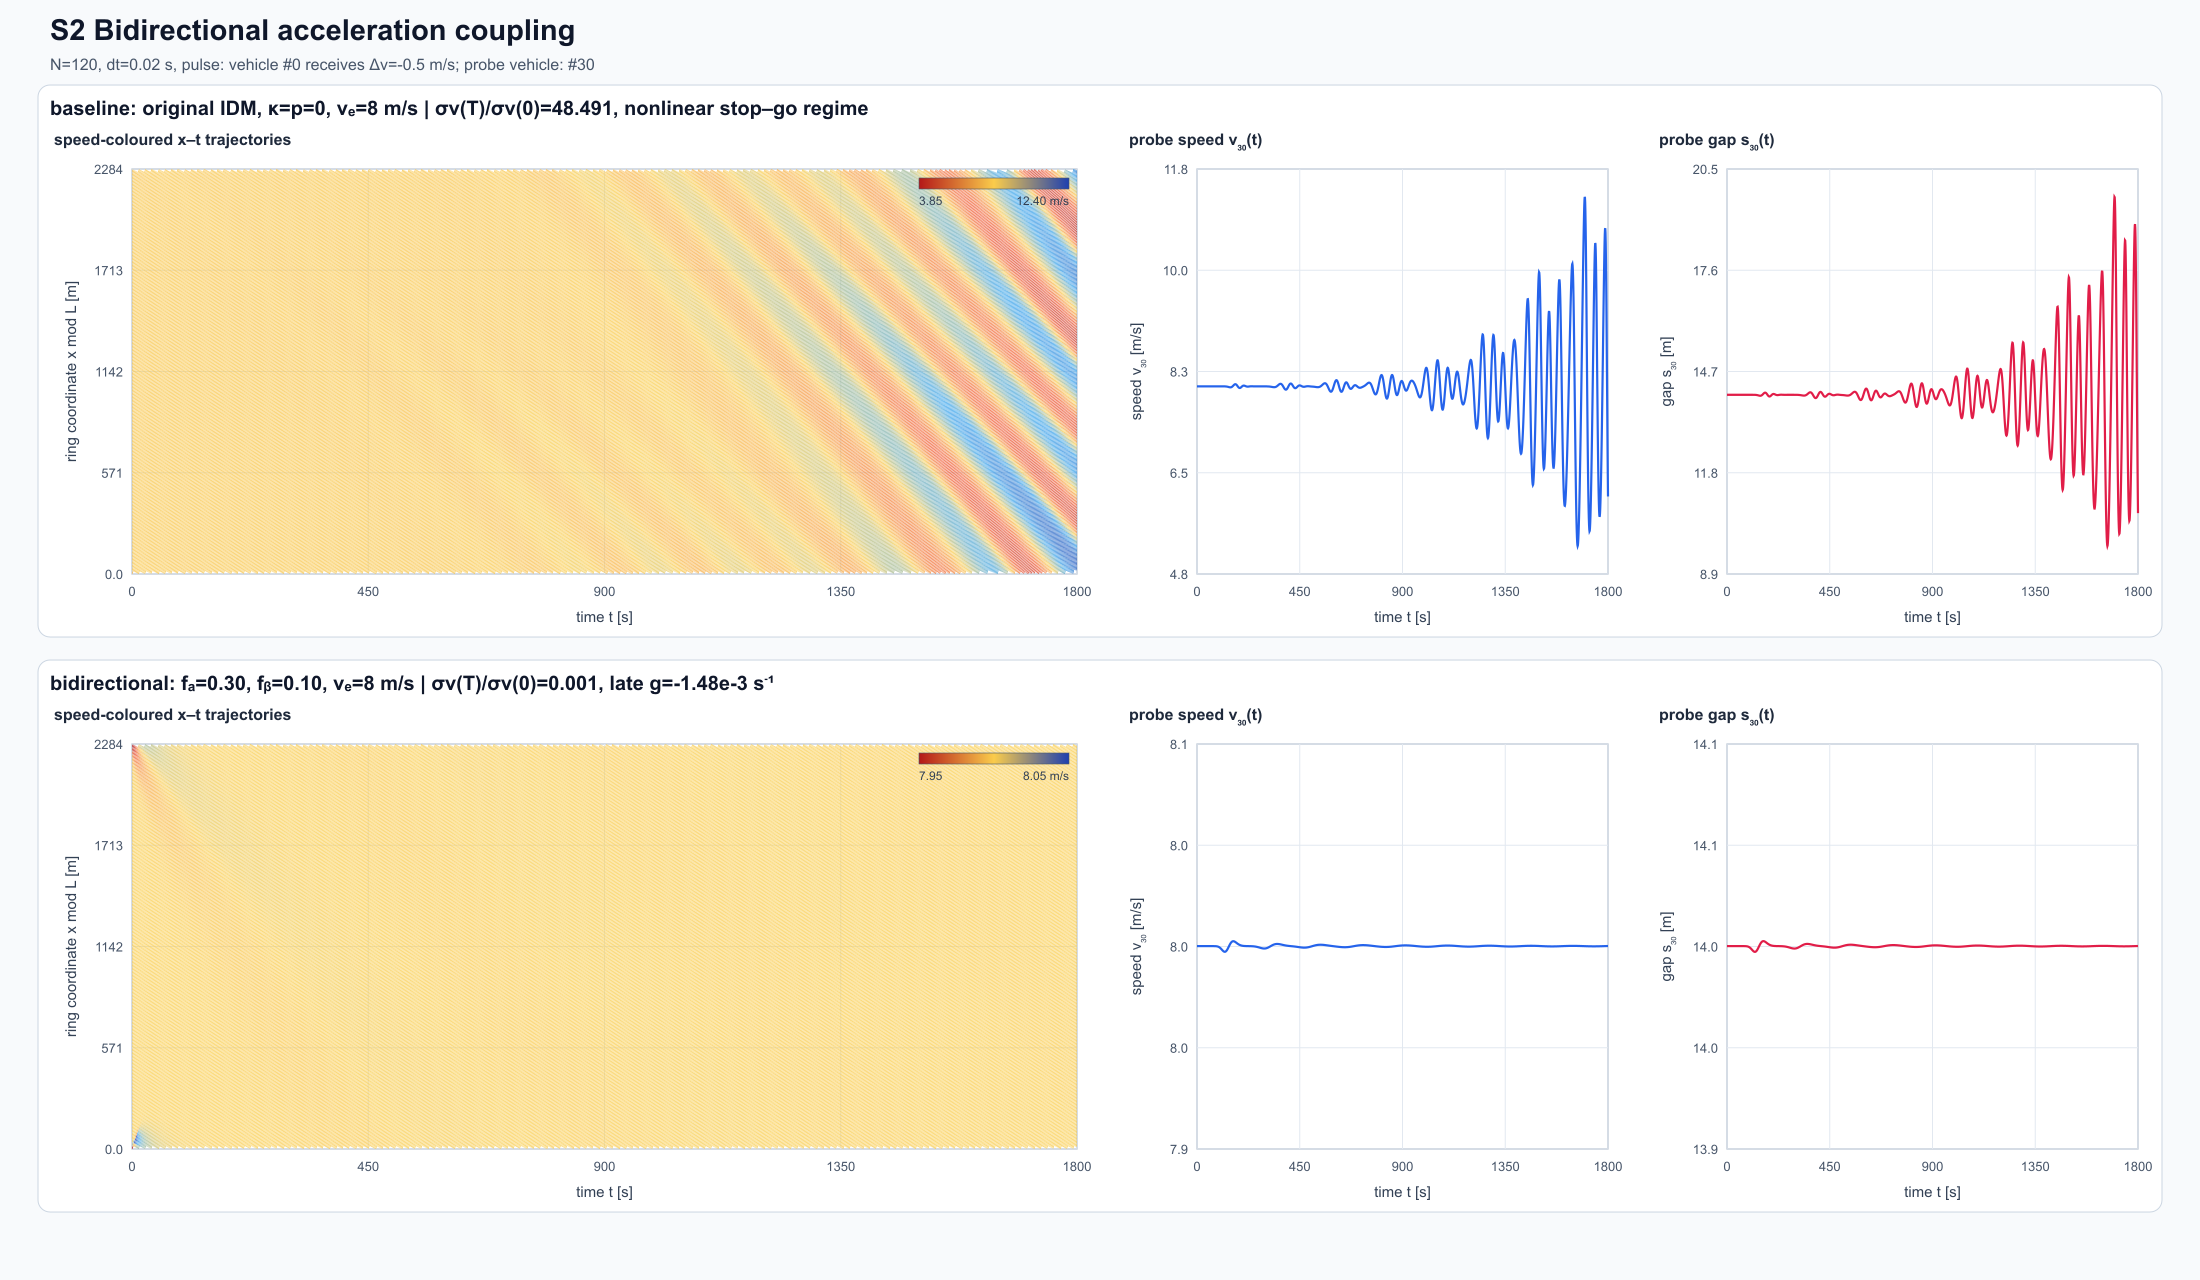
\includegraphics[width=\textwidth]{sim_s2_bilateral_acc.png}
\caption{S2：双向加速度耦合的轨迹对照。}
\label{fig:traj-s2}
\figurenote{S2 双向隐式加速度耦合的时域复核。上行仍是原始 IDM 失稳基准，下行只加入 $(f_a,f_b)=(0.30,0.10)$；车辆数、工作点、扰动和色标均不变。由于每辆车的加速度同时依赖前、后邻车加速度，下行每个 RK4 子步都求解循环线性系统，而不是用上一步加速度显式替代；这避免数值滞后污染稳定性结论。结果显示，上行斜向色带逐圈增强，下行色带在传播中消散，指定车辆的速度与间距峰值也同步缩小。该图不仅证明这一参数点位于图~\ref{fig:bilateral-domain} 的稳定区，还说明复系数谱所预测的负增长率能在完整非线性、隐式耦合仿真中实现。}
\end{figure}

%==================================================================
\sectionwrapup{加入后车加速度后，车辆加速度在同一时刻循环耦合，标量逐车传递函数失效；每个积分子步需解循环线性系统。稳定性由复系数环道特征方程及两条实条件共同决定，不能只看长波门槛。}

\chapter{再推广：多前车与多后车的加速度反馈}
\label{sec:multi}
\chapterguide{多车信息的收益取决于总量还是空间分配}{本章把任意前后向加速度核压缩进复函数 $P(k)$，用零阶矩与一阶矩分离长波预算和有限波长代价。目标是从“看得更多”推进到可计算的增益分配原则。}

本章暂不考虑延迟。

\section{模型：指数衰减权重}
\sectionstudy{model}{模型：指数衰减权重}{lenz1999,feng2019}

自车同时接收前方 $j$ 辆车与后方 $j$ 辆车的加速度，权重按车序指数衰减：
\begin{equation}
\dot v_n = F\left(s_n,v_n,\dv_n\right)
+ \sum_{j\ge1} f_a\,\alpha^{\,j-1}\,\dot v_{n-j}
+ \sum_{j\ge1} f_b\,\beta^{\,j-1}\,\dot v_{n+j},
\qquad 0\le\alpha,\beta<1
\end{equation}

$f_a,f_b$ 是\textbf{最近邻}的反馈系数，$\alpha,\beta$ 是衰减因子。总反馈量为
\begin{equation}
\sum_{j\ge1}f_a\alpha^{j-1} = \frac{f_a}{1-\alpha},
\qquad
\sum_{j\ge1}f_b\beta^{j-1} = \frac{f_b}{1-\beta}
\end{equation}

\section{空间 Fourier：耦合函数 \texorpdfstring{$P(k)$}{P(k)}}
\sectionstudy{theory}{空间 Fourier：耦合函数 \texorpdfstring{$P(k)$}{P(k)}}{lenz1999,feng2019}

代入 $y_{n\mp j}=y_n e^{\mp ijk}$，两个几何级数都可求和：
\begin{equation}
\sum_{j\ge1}f_a\alpha^{j-1}e^{-ijk} = \frac{f_a e^{-ik}}{1-\alpha e^{-ik}},
\qquad
\sum_{j\ge1}f_b\beta^{j-1}e^{ijk} = \frac{f_b e^{ik}}{1-\beta e^{ik}}
\end{equation}

于是特征方程形式与 第~\ref{sec:bilat}~章 完全相同：
\begin{equation}
P(k)\,\lambda^2 - Q(k)\,\lambda - R(k) = 0,
\qquad
P(k) = 1 - \frac{f_a e^{-ik}}{1-\alpha e^{-ik}} - \frac{f_b e^{ik}}{1-\beta e^{ik}}
\end{equation}
而 $Q=f_v+f_{v_l}e^{-ik}$、$R=f_s(e^{-ik}-1)$ 的结构保持不变。

\begin{tcolorbox}[notebox]
\textbf{所有加速度耦合的复杂性都被压缩进了一个复函数 $P(k)$。} 这提示我们：把 第~\ref{sec:bilat}~章 的推导对\textbf{任意} $P$ 重做一遍，就能一次性覆盖所有情形。
\end{tcolorbox}

\section{统一框架：任意加速度核的两个条件}
\sectionstudy{theory}{统一框架：任意加速度核的两个条件}{lenz1999,feng2019}

设加速度耦合核的空间变换为
\begin{equation}
P(k) = 1 - \sum_{j\ge1}a_j e^{-ijk} - \sum_{j\ge1}b_j e^{ijk} \;\equiv\; P_r(k) + i\,P_i(k)
\end{equation}

对一般复数 $P$ 重做 Bilharz 判据（记 $u=\cos k$、$q=\sin k$），可得

\begin{tcolorbox}[keybox,title=\textbf{条件 I}]
\begin{equation}
\Pi(k) = P_i\,f_{v_l}\,q - P_r\left(f_v + f_{v_l}u\right) \;>\; 0
\end{equation}
\end{tcolorbox}

\begin{tcolorbox}[keybox,title=\textbf{条件 II}]
\begin{equation}
\begin{aligned}
\widetilde W(k)={}&P_r\Big[f_v^2-f_{v_l}^2u+f_vf_{v_l}(u-1)-f_s(1+u)P_r\Big]\\
&+P_i q\Big[2f_sP_r-f_{v_l}(f_v-f_{v_l})\Big]
-f_s(1-u)P_i^2>0
\end{aligned}
\end{equation}
\end{tcolorbox}

两个端点（此处 $q=0$，且本书所考虑的核均满足 $P_i\propto q$，故 $P_i=0$）：
\begin{align}
\Pi\big|_{k=0} &= -P(0)\left(f_v+f_{v_l}\right) \\
\widetilde W\big|_{k=0} &= P(0)\Big[f_v^2 - f_{v_l}^2 - 2f_s\,P(0)\Big]
\label{eq:Wend}\\
\widetilde W\big|_{k=\pi} &= P(\pi)\left(f_v-f_{v_l}\right)^2
\end{align}

\begin{tcolorbox}[notebox,title=\textbf{向下兼容检验}]
\begin{itemize}[leftmargin=1.2em,itemsep=2pt]
\item $P\equiv1$（无加速度反馈）：$\widetilde W = \left(f_v^2-f_vf_{v_l}-f_s\right)+u\left(f_vf_{v_l}-f_{v_l}^2-f_s\right)$，即 第~\ref{sec:string}~章 的基准结果。
\item $P=1-f_ae^{-ik}$：即 第~\ref{sec:lead}~章。
\item $P=1-f_ae^{-ik}-f_be^{ik}$：即 第~\ref{sec:bilat}~章，$P(0)=1-\sigma$，两个端点公式与那里逐字吻合。
\end{itemize}
\end{tcolorbox}

\section{指数衰减核的 \texorpdfstring{$P_r$ 与 $P_i$}{实部与虚部}}
\sectionstudy{theory}{指数衰减核的 \texorpdfstring{$P_r$ 与 $P_i$}{实部与虚部}}{lenz1999,feng2019}

关键是这个恒等式（分子分母同乘共轭）：
\begin{equation}
\frac{e^{-ik}}{1-\alpha e^{-ik}} = \frac{\left(\cos k-\alpha\right) - i\sin k}{1-2\alpha\cos k+\alpha^2}
\end{equation}

记 $D_\alpha = 1-2\alpha u+\alpha^2>0$、$D_\beta = 1-2\beta u+\beta^2>0$（$|\alpha|,|\beta|<1$ 时恒正），则

\begin{tcolorbox}[keybox]
\begin{equation}
P_r = 1 - \frac{f_a\left(u-\alpha\right)}{D_\alpha} - \frac{f_b\left(u-\beta\right)}{D_\beta},
\qquad
P_i = s\left(\frac{f_a}{D_\alpha} - \frac{f_b}{D_\beta}\right)
\end{equation}
\end{tcolorbox}

代入 $u=1$（$D_\alpha=(1-\alpha)^2$）与 $u=-1$（$D_\alpha=(1+\alpha)^2$）：
\begin{equation}
P(0) = 1 - \underbrace{\left(\frac{f_a}{1-\alpha} + \frac{f_b}{1-\beta}\right)}_{\textstyle \sigma_{\rm eff}},
\qquad
P(\pi) = 1 + \frac{f_a}{1+\alpha} + \frac{f_b}{1+\beta}
\end{equation}

\section{闭式结论}
\sectionstudy{theory}{闭式结论}{lenz1999,feng2019}

\begin{tcolorbox}[keybox,title=\textbf{(A) 总反馈量上界}]
由 $\Pi(0)>0$ 且 $f_v+f_{v_l}<0$：
\begin{equation}
\sigma_{\rm eff} = \frac{f_a}{1-\alpha} + \frac{f_b}{1-\beta} \;<\; 1
\end{equation}
\end{tcolorbox}

\begin{tcolorbox}[keybox,title=\textbf{(B) 短波条件}]
由 $\widetilde W(\pi)>0$：
\begin{equation}
1 + \frac{f_a}{1+\alpha} + \frac{f_b}{1+\beta} \;>\; 0
\end{equation}
$f_a,f_b\ge0$ 时自动满足。
\end{tcolorbox}

\begin{tcolorbox}[keybox,title=\textbf{(C) 长波条件：只依赖 $\sigma_{\rm eff}$}]
由式~\eqref{eq:Wend} 及 $P(0)>0$：
\begin{equation}
\frac{1}{2}\left(f_v^2-f_{v_l}^2\right) \;\ge\; \left(1-\sigma_{\rm eff}\right)f_s
\end{equation}
\textbf{无论反馈是集中在最近邻还是摊到很多辆车上，长波门槛只看总量 $\sigma_{\rm eff}$。} 这是 第~\ref{sec:bilat}~章 结论 (B) 的自然推广。
\end{tcolorbox}

\begin{tcolorbox}[keybox,title=\textbf{(D) 有限波长条件}]
还需 $\Pi(k)>0$ 与 $\widetilde W(k)>0$ 在 $k\in(0,\pi]$ 内成立。$\alpha,\beta$ 出现在 $D_\alpha,D_\beta$ 的分母上，使 $\widetilde W$ 不再是多项式，一般需数值扫描。
\end{tcolorbox}

\section{数值算例}
\sectionstudy{experiment}{数值算例}{lenz1999,feng2019}

仍用第~\ref{sec:num}~章 IDM 参数，要求\textbf{全速域}线稳定。全速域最苛刻的长波门槛为
\begin{equation}
\sigma_c = \max_{v_e}\left[1-\frac{f_v^2-f_{v_l}^2}{2f_s}\right] = 0.1336
\end{equation}

\begin{figure}[htbp]
\centering
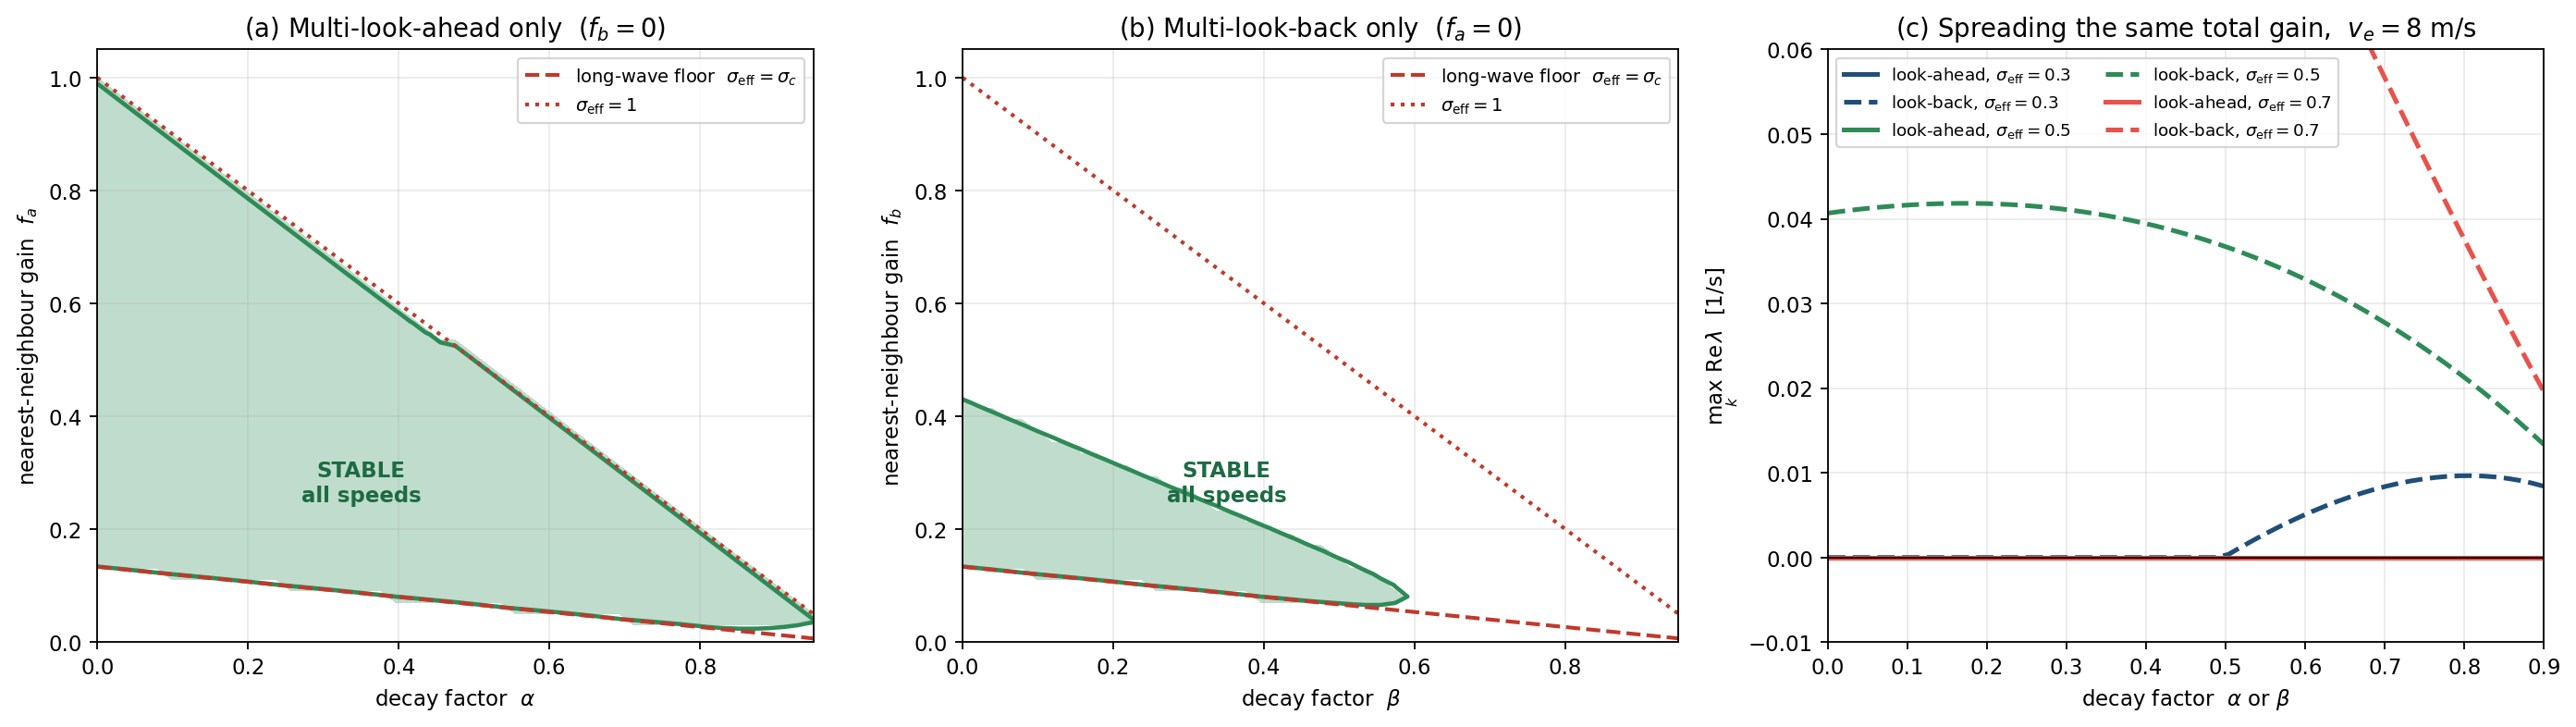
\includegraphics[width=\textwidth]{fig5.png}
\caption{多前车与多后车反馈的稳定域。}
\label{fig:multi-domain}
\figurenote{多前车与多后车指数核的稳定域比较。左图只保留前视核，稳定区域随衰减因子和最近邻增益变化，并由总反馈下限与高频上限两条闭式边界夹住；这说明前方信息可以在总量不变时分摊到更多车辆。中图只保留回望核，稳定区域明显收缩，当衰减过慢、远处后车权重累积过大时稳定解完全消失，表明“看得更远”在回望方向可能放大错误相位。右图固定零阶总量，只改变核的空间范围：所有曲线在 $k\to0$ 具有相同起点，但有限波数处明显分离，直接显示一阶矩而非车辆数量本身控制中短波裕度。该图证明多车通信的评价不能只写“接收了几辆车”，还必须报告方向、每个权重以及核矩。}
\end{figure}

\textbf{(1) 多前车反馈（$f_b=0$）——完全良性.} 可行域就是
\begin{equation}
\sigma_c\left(1-\alpha\right) \;\le\; f_a \;\lesssim\; 1-\alpha
\end{equation}
即条件 (A) 与 (C) 已经几乎充分，有限波长条件基本不额外收紧。

这带来一个很实用的推论：\textbf{摊到多车可以把单车增益压得很低}。例如 $\alpha=0.8$ 时只需
\begin{equation}
f_a \ge 0.1336\times0.2 = 0.027
\end{equation}
即对最近前车的加速度只需 $2.7\%$ 的前馈增益，就能消除整条走停波带——对传感精度和通信带宽的要求大大放宽。

\textbf{(2) 多后车反馈（$f_a=0$）——看得越远越糟.} 可行域被一条弯曲的上边界截断（$\beta=0$ 时 $f_b\lesssim0.43$，与 第~\ref{sec:bilat}~章 一致），且 $\beta$ 超过约 $0.58$ 后\textbf{无论增益取多少都无法全速域稳定}。

\begin{center}
\captionof{table}{多前车与多后车反馈的全速域性质。}
\label{tab:multi-front-rear-comparison}
\begin{tabular}{rcc}
\toprule
& 多前车（$\alpha$） & 多后车（$\beta$） \\
\midrule
衰减因子的可用范围 & 全部 $[0,1)$ & $\lesssim0.58$ \\
上界是否由闭式给出 & 基本是（$\sigma_{\rm eff}<1$） & 否，须数值扫描 \\
固定 $\sigma_{\rm eff}$ 时增大衰减因子 & 无影响（始终稳定） & 恶化 \\
\bottomrule
\end{tabular}
\end{center}
\tabletext{tab:multi-front-rear-comparison}{前向和后向指数核在可用衰减范围、闭式上界和远距分配效应上的差别。前向总量可安全摊薄，后向信息范围过大则会触发有限波长失稳。}

\section{数值验证 E3：同一总量，不同空间分配}
\sectionstudy{experiment}{数值验证 E3：同一总量，不同空间分配}{lenz1999,feng2019}

在 $N=120$、$v_e=8$ m/s 上把指数核截断到前／后方 20 辆车，并直接扫描全部离散波数。纯多前车取 $(\alpha,f_a)=(0.8,0.027)$，其无限核总量为 $0.135$；纯多后车取 $(\beta,f_b)=(0.5,0.08)$，总量为 $0.16$。

\begin{center}
\small
\captionof{table}{E3 多邻车核的总反馈量与最右根。}
\label{tab:e3-multi-neighbour}
\begin{tabular}{p{3.7cm}p{3.0cm}p{3.6cm}p{2.8cm}}
\toprule
\textbf{核} & \textbf{总反馈量} & \textbf{$\max\operatorname{Re}\lambda$ [s$^{-1}$]} & \textbf{当前工况} \\
\midrule
多前车 $\alpha=0.8$ & $0.135$ & $-1.17\times10^{-5}$ & 临界侧稳定 \\
多后车 $\beta=0.5$ & $0.160$ & $-1.42\times10^{-4}$ & 稳定 \\
\bottomrule
\end{tabular}
\end{center}
\tabletext{tab:e3-multi-neighbour}{多前车和多后车核在选定工作点的总反馈量与增长率。两者在该点都稳定，但后向核仍需全速域、全波数检查，不能由单点结果外推。}

第二行并不意味着多后车在全速域都安全：继续扫描 $v_e$ 与 $\beta$ 后，$\beta\gtrsim0.58$ 时可行窗口消失。该对照说明\textbf{单一工作点稳定}与\textbf{全速域稳定}是两个不同命题；零阶矩足以解释前者的长波符号，却不能替代后者的有限波长扫描。

\begin{tcolorbox}[resultbox,title=\textbf{验证结论}]
向前分摊时，最近邻增益仅 $0.027$ 就能把当前最右根推到左半平面，验证了“总量不变、单车负担按 $1-\alpha$ 摊薄”。向后分摊虽可在选定工况稳定，但必须额外报告全波数、全速度扫描，验证有限波长上界没有被穿越。
\end{tcolorbox}

\section{具体轨迹结果：多前车信息的空间分摊}
\sectionstudy{experiment}{具体轨迹结果：多前车信息的空间分摊}{lenz1999,feng2019}

图~\ref{fig:traj-s3} 固定 $v_e=8$ m/s，用 $m=20$、$\alpha=0.8$、$f_a=0.027$ 的指数核替代最近邻反馈。基准 IDM 的 $\sigma_v(1800)/\sigma_v(0)=48.49$，多前车反馈下则为 $0.0377$，末段斜率为 $-3.06\times10^{-4}$ s$^{-1}$。探针车速度限制在 $7.9918$--$8.0143$ m/s、间距限制在 $14.0214$--$14.0592$ m，说明分摊后的弱单车增益仍能使扰动逐圈消散。

\begin{figure}[htbp]
\centering
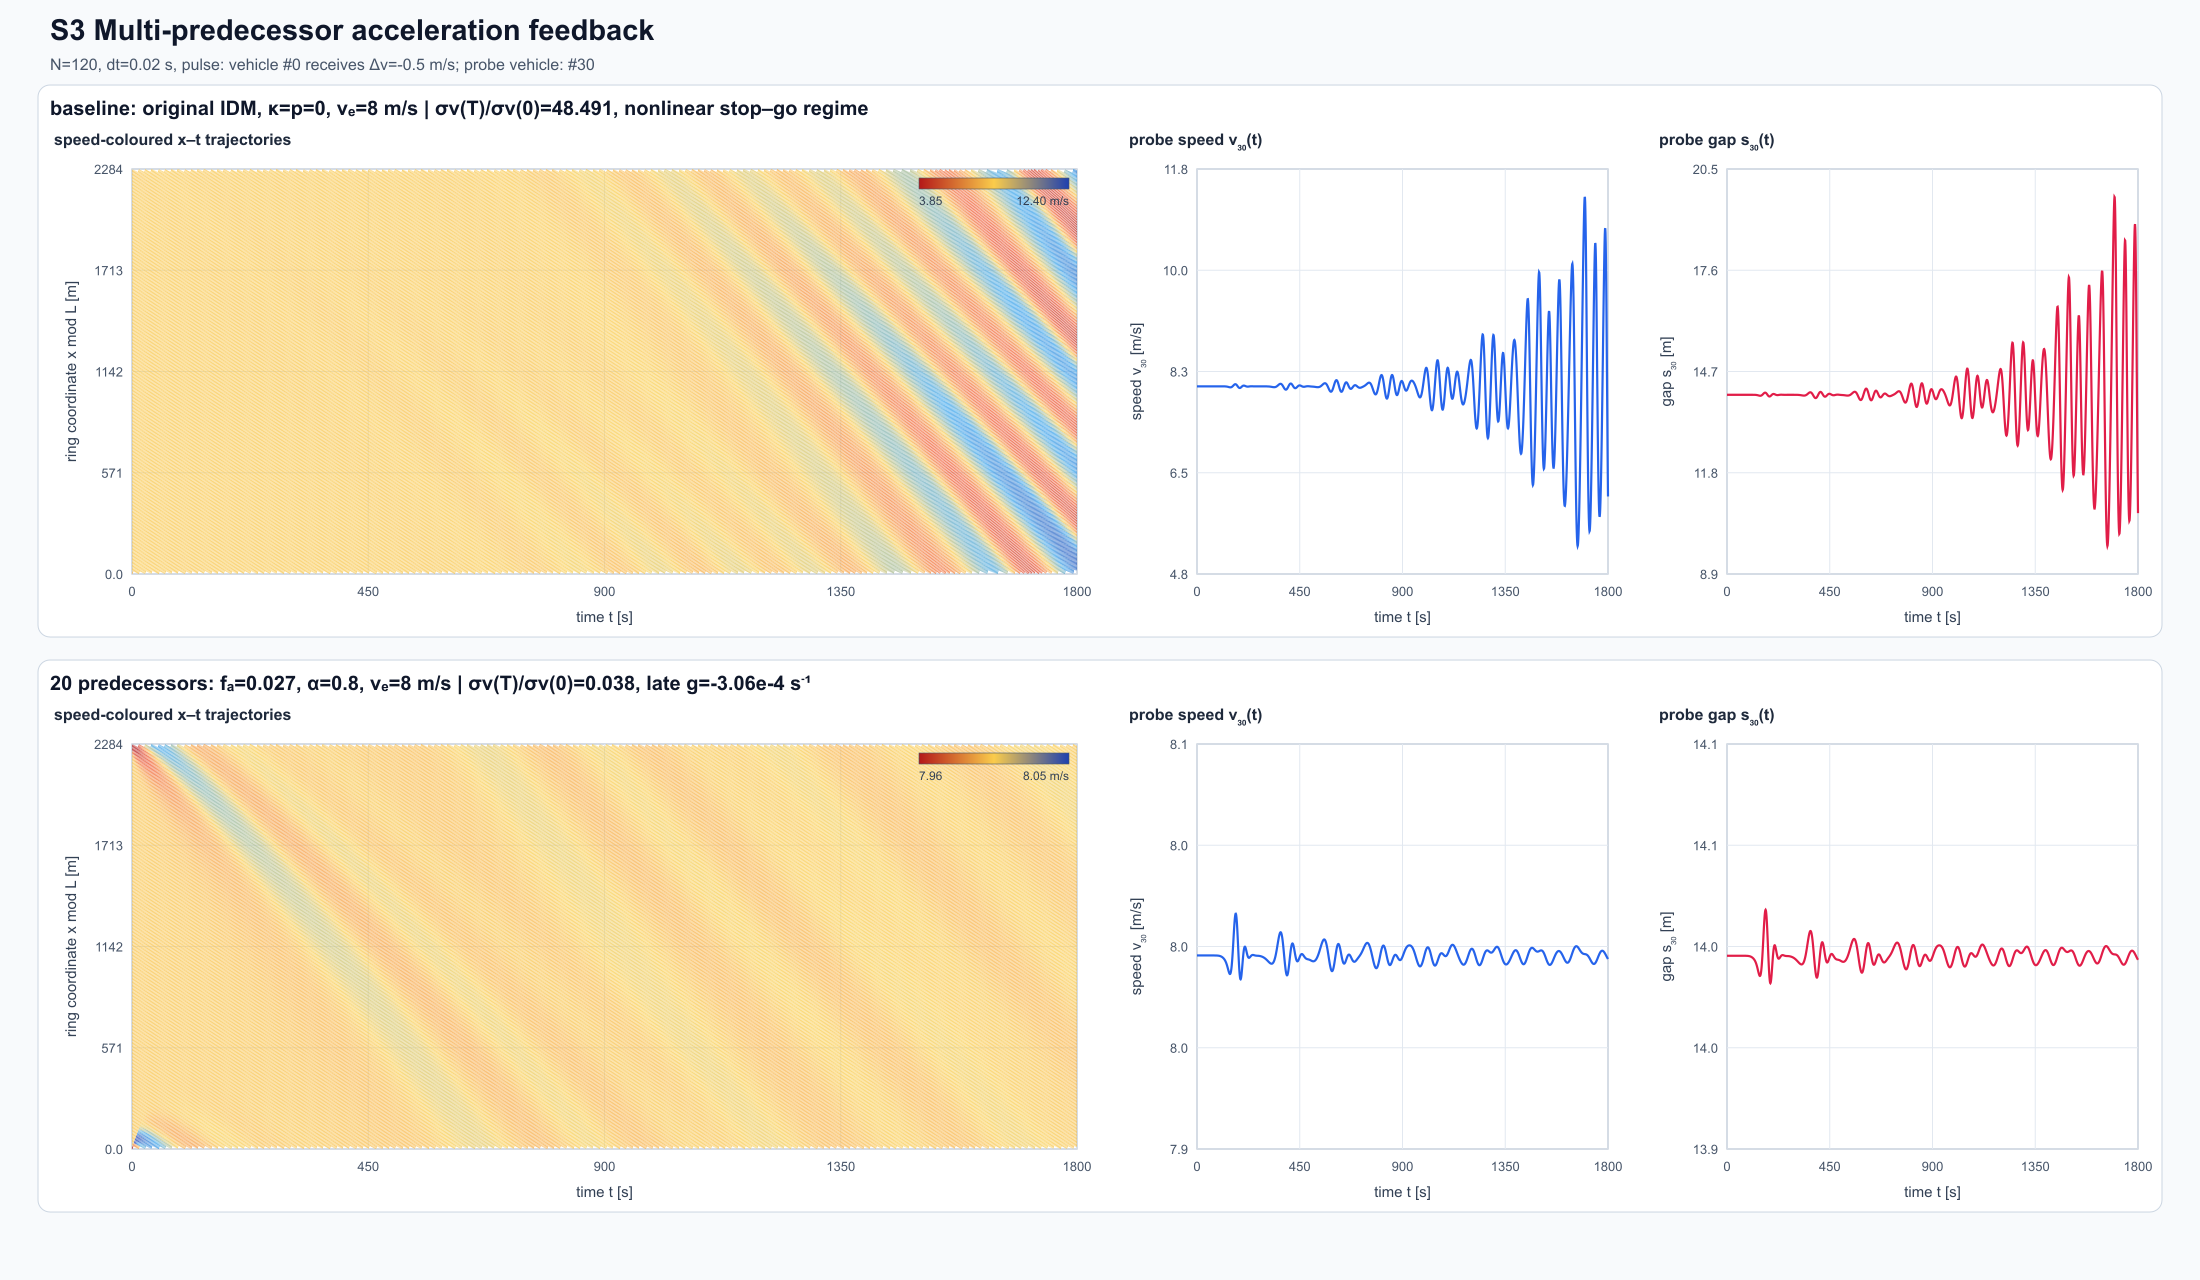
\includegraphics[width=\textwidth]{sim_s3_multi_front.png}
\caption{S3：多前车反馈的轨迹对照。}
\label{fig:traj-s3}
\figurenote{S3 把多前车稳定域转化为可观察的交通波演化。下行让每辆车接收前方 20 辆车的加速度，权重按 $\alpha=0.8$ 指数衰减，最近邻系数仅为 $f_a=0.027$；上行仍是同一失稳基准。虽然单个最近邻增益远小于 S1 的 $0.15$，指数核的总量约为 $f_a/(1-\alpha)$，足以越过长波门槛；下行色带逐圈变淡、指定车辆速度和间距回到平衡，验证“总量可向多辆前车分摊”。与上行形成的走停波相比，下行没有出现由远距信息引起的新短波纹理，说明所选衰减核同时通过了有限波长检查。该图证明多前车通信的收益不是更大的单车控制动作，而是利用空间分布的较小增益共同提供稳定预算。}
\end{figure}

\section{为什么前视与回望如此不对称}
\sectionstudy{theory}{为什么前视与回望如此不对称}{lenz1999,feng2019}
\label{sub:asym}

前面的数值差异有一个非常干净的解释。把 $P$ 按 Euler 公式拆开：
\begin{equation}
P(k) = 1 - \sum_{j\ge1}\left(a_j e^{-ijk} + b_j e^{ijk}\right)
\end{equation}
\begin{tcolorbox}[keybox]
\begin{equation}
P_r = 1 - \sum_{j\ge1}\left(a_j+b_j\right)\cos jk,
\qquad
P_i = \sum_{j\ge1}\left(a_j-b_j\right)\sin jk
\end{equation}
\end{tcolorbox}

\textbf{$P_r$ 只看耦合核的对称部分，$P_i$ 只看反对称部分。} 于是：把同样的增益从前视换成回望，$P_r$ \textbf{一字不变}，只有 $P_i$ 整体反号。

再看条件 II 中 $P_i$ 的系数：
\begin{equation}
\widetilde W \;\supset\; P_i\,s\underbrace{\Big[2f_sP_r + f_{v_l}\left(f_{v_l}-f_v\right)\Big]}_{\textstyle >\,0\ \text{恒成立}}
\end{equation}
（因 $f_v<0<f_{v_l}$，故 $f_{v_l}-f_v>0$。）所以

\begin{tcolorbox}[notebox]
\textbf{前视（$P_i>0$）加分，回望（$P_i<0$）扣分，而且大小完全对称。} 两者唯一的区别就是这一个符号。
\end{tcolorbox}

\subsection{矩展开：好处是零阶矩，坏处是一阶矩}

在 $k\to0$ 附近展开（$u=1-k^2/2$、$s=k$），记耦合核的各阶矩
\begin{equation}
m_0 = \sum_j\left(a_j+b_j\right) = \sigma_{\rm eff},
\qquad
m_1 = \sum_j j\left(a_j-b_j\right),
\qquad
m_2 = \sum_j j^2\left(a_j+b_j\right)
\end{equation}
则 $P_r \approx \left(1-m_0\right) + \tfrac12 m_2k^2$、$P_i\approx m_1k$，代入得
\begin{equation}
\widetilde W(k) \;\approx\; \underbrace{P_0\left(f_v^2-f_{v_l}^2-2f_sP_0\right)}_{\text{只含 }m_0}
\;+\; k^2\Big\{\underbrace{m_1\left[2f_sP_0+f_{v_l}\left(f_{v_l}-f_v\right)\right]}_{\text{反对称，符号即胜负}} + \big(\text{只含 }m_0,m_2\text{ 的项}\big)\Big\}
\end{equation}
其中 $P_0=1-m_0$。

\begin{tcolorbox}[keybox,title=\textbf{结论}]
\begin{itemize}[leftmargin=1.2em,itemsep=3pt]
\item \textbf{好处（放宽长波门槛）只依赖零阶矩 $m_0=\sigma_{\rm eff}$}，与前后分配无关；
\item \textbf{坏处（$k^2$ 项被压低）依赖一阶矩 $m_1$}，前视贡献正、回望贡献负。
\end{itemize}
\end{tcolorbox}

对指数衰减核：
\begin{equation}
\sum_j j\,a_j = \frac{f_a}{\left(1-\alpha\right)^2} = \frac{\sigma_a}{1-\alpha},
\qquad
\sum_j j\,b_j = \frac{f_b}{\left(1-\beta\right)^2} = \frac{\sigma_b}{1-\beta}
\end{equation}
其中 $\sigma_a=f_a/(1-\alpha)$、$\sigma_b=f_b/(1-\beta)$ 是各自的总量，$1/(1-\alpha)$、$1/(1-\beta)$ 恰是\textbf{平均观测距离}（单位：车）。

\begin{tcolorbox}[notebox,title=\textbf{这就回答了"为什么回望一辆行、多辆不行"}]
固定总量 $\sigma_b$ 不变时：
\[
\text{零阶矩（好处）} = \sigma_b \ \text{不变},
\qquad
\text{一阶矩（坏处）} = \frac{\sigma_b}{1-\beta}\ \text{被放大 } \frac{1}{1-\beta}\ \text{倍}
\]
\textbf{回望一辆}（$\beta=0$）时平均距离为 1，扣分最小，零阶矩的好处占优，净收益为正；\textbf{回望多辆}时好处一点没涨，扣分却按 $1/(1-\beta)$ 膨胀，于是翻负。前视方向则相反——摊得越远，$m_1$ 越大，$k^2$ 项越被抬高，所以怎么摊都安全。
\end{tcolorbox}

\textbf{数值印证.} 取 $v_e=8$ m/s、$\sigma_{\rm eff}=0.3$、衰减因子 $0.85$（即最近邻增益 $0.045$）：

\begin{center}
\captionof{table}{固定零阶矩时前视与回望的一阶矩效应。}
\label{tab:first-moment-effect}
\begin{tabular}{lccc}
\toprule
& $m_1$ & $k^2$ 系数 & $\min_k\widetilde W$ \\
\midrule
纯前视 $\alpha=0.85$ & $+2.00$ & $-0.184$ & $+0.029$（稳定）\\
纯回望 $\beta=0.85$  & $-2.00$ & $-3.110$ & $-0.027$（失稳）\\
\bottomrule
\end{tabular}
\end{center}
\tabletext{tab:first-moment-effect}{相同 $m_0$ 下纯前视与纯回望的 $m_1$、$k^2$ 系数和最小裕度。两行之差精确对应一阶矩项，证明有限波长差异来自方向相位而非总增益。}

两者的 $P_r$、$m_0$、$m_2$ 完全相同，$\widetilde W(0)$ 也都是 $+0.0333$；$k^2$ 系数之差恰为
\begin{equation}
2m_1\left[2f_sP_0+f_{v_l}\left(f_{v_l}-f_v\right)\right] = 2\times2.00\times0.732 = 2.93
\end{equation}
与表中 $-0.184-(-3.110)=2.93$ 精确吻合。

\subsection{物理图像}

$\sin(jk)$ 正是隔 $j$ 辆车的\textbf{相位差}。走停波沿车队\textbf{向后}传播（前车 $\to$ 自车 $\to$ 后车），因此
\begin{itemize}[leftmargin=1.4em,itemsep=3pt]
\item $\dot v_{n-j}$ 是扰动\textbf{即将传到自己}的预览信息——相位超前，越往前看超前量越大，越有利；
\item $\dot v_{n+j}$ 是扰动\textbf{已经离开自己}之后的回授——相位滞后，越往后看滞后量越大，等于在环路里塞进更长的延迟，越有害。
\end{itemize}
最近的那一辆后车（$j=1$）滞后最小，其"提供总反馈量"的好处还压得住"相位滞后"的坏处；再往后就压不住了。

\section{回望取负号：文献中的常用约定}
\sectionstudy{theory}{回望取负号：文献中的常用约定}{lenz1999,feng2019}
\label{sub:negfb}

\subsection{先核对符号约定}

本书的约定是 $f_b = \partial f/\partial\dot v_{n+1}$，前面的数值算例默认 $f_b>0$。文献中常见的写法有两类，映射到本书符号时结果完全不同，套用前务必核对：

\begin{center}
\captionof{table}{两类后车加速度写法与本书符号的对应。}
\label{tab:rear-acceleration-signs}
\begin{tabular}{p{6.4cm}p{4.2cm}p{3.4cm}}
\toprule
文献写法 & 本书等效 $f_b$ & 符号 \\
\midrule
$\dot v_n = F + \lambda_a\dot v_{n-1} - \lambda_b\dot v_{n+1}$ & $f_b = -\lambda_b$ & \textbf{负} \\[4pt]
$\dot v_n = F + \gamma_b\left(\dot v_{n+1}-\dot v_n\right)$（相对加速度） & $f_b = \dfrac{\gamma_b}{1+\gamma_b}$，且 $f_s,f_v,f_{v_l}$ 同除 $1+\gamma_b$ & \textbf{正} \\
\bottomrule
\end{tabular}
\end{center}
\tabletext{tab:rear-acceleration-signs}{文献中绝对后车加速度与相对加速度两种写法映射到 $f_b$ 后的符号。该对照防止把“负反馈”的语言标签直接等同于本书参数的正负号。}

若论文把后视项作为\textbf{负反馈}处理，对应的就是本书的 $f_b<0$。

\subsection{矩框架下负 $f_b$ 做了什么}

回到 \S\ref{sub:asym} 的两个矩：
\begin{equation}
m_0 = \frac{f_a}{1-\alpha}+\frac{f_b}{1-\beta} = \sigma_{\rm eff},
\qquad
m_1 = \frac{f_a}{\left(1-\alpha\right)^2} - \frac{f_b}{\left(1-\beta\right)^2}
\end{equation}

$f_b<0$ 时两者同时改变，且方向相反：

\begin{tcolorbox}[keybox,title=\textbf{负回望＝拿长波裕度换有限波长裕度}]
\begin{itemize}[leftmargin=1.2em,itemsep=3pt]
\item $m_0$ \textbf{减小} $\Rightarrow$ 长波条件 $\tfrac12(f_v^2-f_{v_l}^2)\ge(1-m_0)f_s$ 变紧（不利）；
\item $m_1$ \textbf{增大}（因 $-f_b/(1-\beta)^2>0$）$\Rightarrow$ $k^2$ 项被抬高（有利）。
\end{itemize}
恰好是 $f_b>0$ 时的镜像。
\end{tcolorbox}

于是"该取正还是取负"完全取决于\textbf{瓶颈在哪一侧}：若 $\sigma_{\rm eff}$ 本来就不够（长波是瓶颈），必须用正 $f_b$ 补总量；若前视已经把 $\sigma_{\rm eff}$ 撑得足够高，瓶颈转到有限波长，就该用负 $f_b$。

\subsection{数值算例}

\begin{figure}[htbp]
\centering
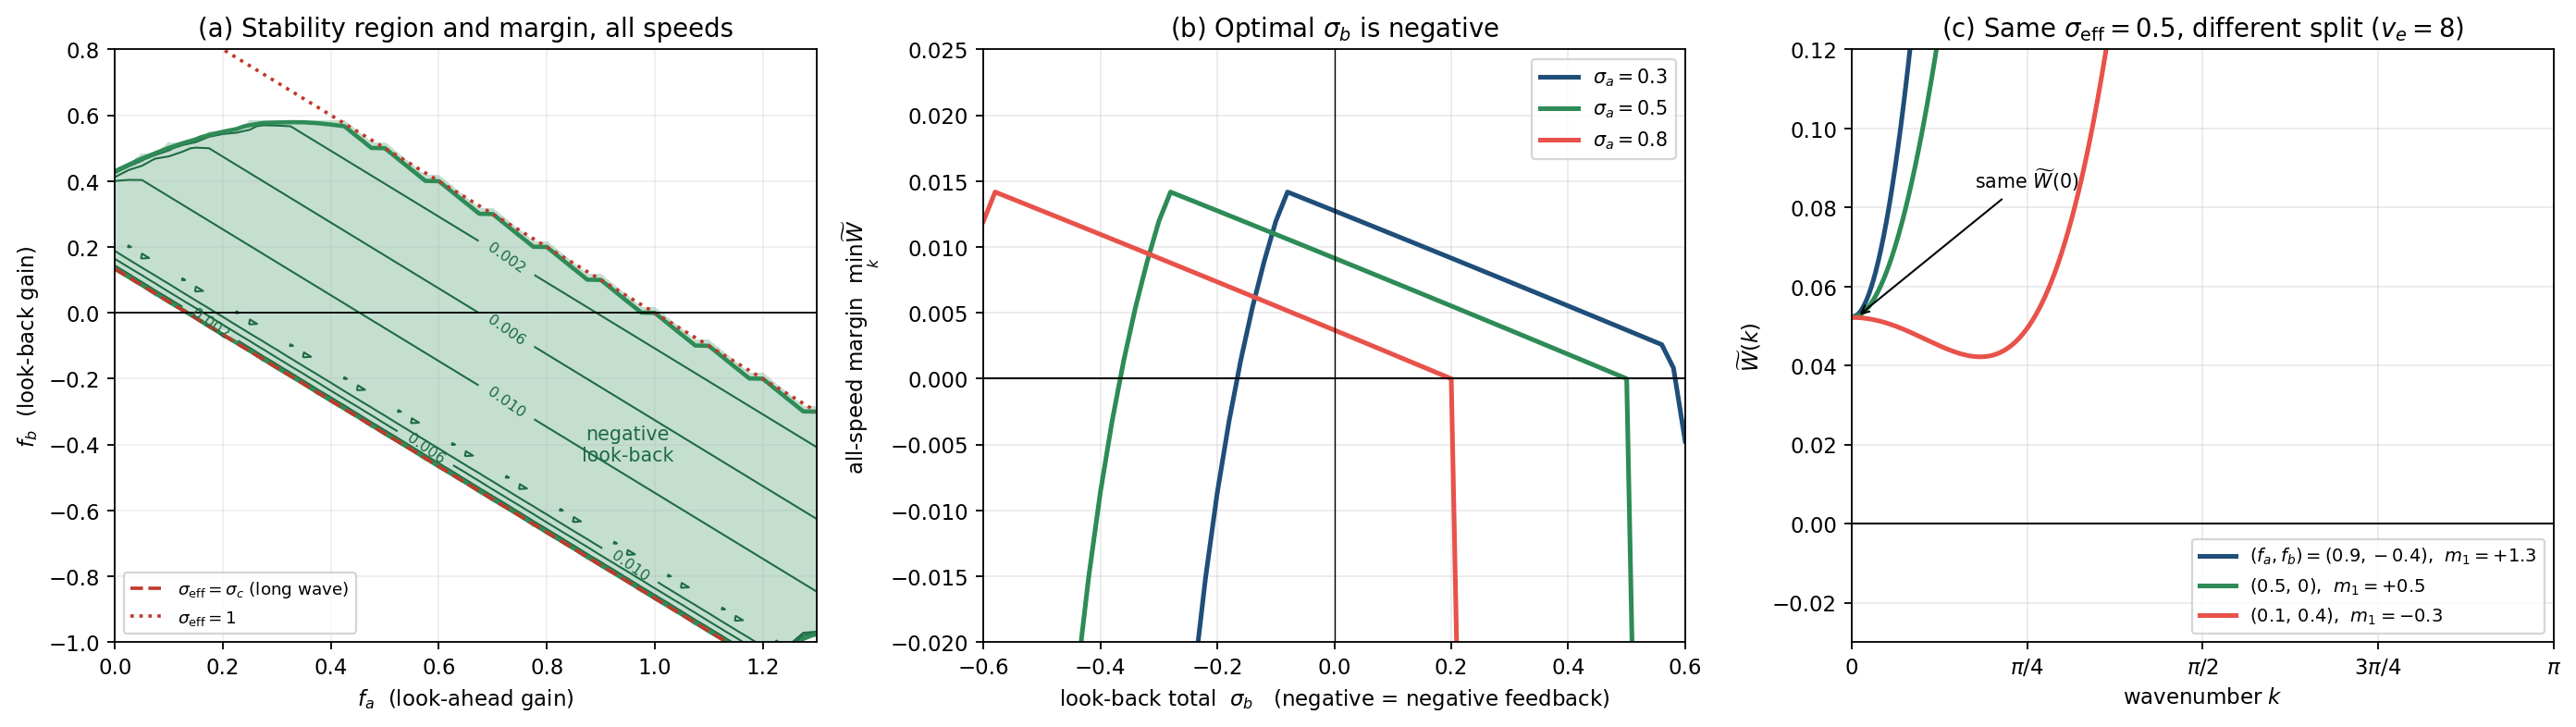
\includegraphics[width=\textwidth]{fig6.png}
\caption{多邻车反馈的裕度、最优分配与矩效应。}
\label{fig:moment-domain}
\figurenote{反馈符号与空间矩对全速度域稳定性的分层作用。左图把最坏工作点、最坏波数下的裕度投影到前视和回望反馈平面，边界显示适量负号回望可以与前视形成阻尼，但过大时又引入有限波长失稳。中图固定前视总量后扫描回望量，曲线的内部最大值说明“回望越多越好”和“完全不回望”都不是一般结论，最优值来自相位补偿与非局部副作用的平衡。右图保持 $\sigma_{\rm eff}$ 不变，仅改变核的一阶矩；三条曲线在 $k=0$ 重合，证明零阶总量决定长波门槛，而有限 $k$ 处分离并出现不同最低点，证明观测距离和方向控制中短波安全余量。该图把“前视好、回望差”的口号细化为可计算条件：零阶矩回答能否跨过长波边界，一阶矩回答跨过以后是否会在有限波长处重新失稳。}
\end{figure}

三条可直接使用的结论：

\begin{itemize}[leftmargin=1.4em,itemsep=4pt]
\item \textbf{带内裕度基本只由 $\sigma_{\rm eff}$ 决定。} 图 (a) 的等值线与 $\sigma_{\rm eff}$ 等值线几乎平行——只要不贴近边界，前后怎么分配几乎不影响裕度大小，只影响\textbf{边界位置}。

\item \textbf{负回望的真正价值是放宽 $f_a$ 的上界。} 硬约束 $\sigma_{\rm eff}<1$ 在只有前视时直接卡住 $f_a<1$。若出于快速跟随、小间距的需要想把 $f_a$ 取大，就得用负 $f_b$ 把总量拉回来：图 (a) 中 $f_b=-0.4$ 时 $f_a$ 可以取到 $1.3$ 以上仍全速域稳定。

\item \textbf{全速域最优总量约为 $\sigma_{\rm eff}\approx0.22$}（使 $P_0\left(f_v^2-f_{v_l}^2-2f_sP_0\right)$ 的全速域最小值最大化，$P_0=1-\sigma_{\rm eff}$），对应裕度 $0.0142$。$\sigma_a=0.3/0.5/0.8$ 时最优 $\sigma_b$ 分别为 $-0.08/-0.28/-0.58$。
\end{itemize}

\subsection{分摊方向也随之反转}

\S\ref{sub:asym} 说过：向后分摊会把 $|m_1|$ 放大 $1/(1-\beta)$ 倍。当 $f_b>0$ 时这放大的是\textbf{扣分}，故有害；当 $f_b<0$ 时放大的是\textbf{加分}，故\textbf{无害甚至有益}。数值上，$\sigma_a=0.5$、$\sigma_b=-0.3$ 时 $\beta$ 从 $0$ 增到 $0.9$，全速域裕度基本不变（略有起伏），完全没有正回望那种 $\beta\gtrsim0.58$ 即崩溃的现象。

\begin{tcolorbox}[notebox,title=\textbf{一句话总结}]
$f_b$ 的符号决定它在\textbf{哪个尺度}上帮忙：正号补长波总量，负号补有限波长相位。文献取负号，通常是因为在那些设定里长波条件已由前视项满足，真正的瓶颈是有限波长的相位裕度。
\end{tcolorbox}

\begin{tcolorbox}[notebox,title=\textbf{工程结论}]
\begin{itemize}[leftmargin=1.2em,itemsep=3pt]
\item \textbf{长波门槛仅由总量决定。} 设计时可先按 $\sigma_{\rm eff}\ge\sigma_c$ 确定总增益预算，再讨论空间分配。
\item \textbf{向前分配不降低长波裕度。} 把同样的总量分配给更多前车，可在保持长波条件不变的同时线性降低最近邻增益——这是多前车感知（V2V 广播、多目标雷达）的直接价值。
\item \textbf{向后分摊有代价（限 $f_b>0$）。} 正的回望反馈摊到远车会在短波段引入失稳，$\beta$ 不宜超过约 $0.5$。若按文献常用的\textbf{负}回望约定（$f_b<0$，见 \S\ref{sub:negfb}），这一结论反转。
\item 合理配置：\textbf{前视用较大的 $\alpha$ 摊薄增益，回望只取最近的一两辆且增益保守}。
\end{itemize}
\end{tcolorbox}

%==================================================================
\sectionwrapup{多车信息由权重核的零阶矩、空间分配和方向不对称共同决定。零阶矩控制长波收益，而远距离回望可能在有限波长处制造新失稳；因此应先分配总增益，再扫描完整波数范围。}

\chapter{澄清：文献中的"后视"多数不是加速度反馈}
\label{sec:reargap}
\chapterguide{为什么不同“后视”研究会给出相反结论}{本章严格区分后车加速度、后向间距和后向相对速度三类反馈通道，说明后向间距反馈不仅能改变增长率，还会改变长波传播速度，从而化解符号约定与物理作用的混淆。}

第~\ref{sec:multi}~章 得到的结论是：单独的\textbf{负}后车\textbf{加速度}反馈会让稳定性变差。这与大量后视文献报告的"后视显著改善稳定性"看似矛盾。矛盾的根源是\textbf{反馈通道不同}。

\section{两种完全不同的"后视"}
\sectionstudy{theory}{两种完全不同的"后视"}{wilsonward2011,stuedli2017}

\begin{center}
\captionof{table}{后车加速度反馈与后向间距反馈的机制差异。}
\label{tab:two-rear-looking-mechanisms}
\begin{tabular}{p{3.2cm}p{5.4cm}p{5.4cm}}
\toprule
& \textbf{后车加速度反馈（第~\ref{sec:lead}~章--第~\ref{sec:multi}~章）} & \textbf{后向间距／相对速度反馈（本章）} \\
\midrule
反馈量 & $\dot v_{n+1}$ & $s_{n+1}=x_n-x_{n+1}-l$，$\ v_{n+1}-v_n$ \\[4pt]
进入哪一项 & 只改 $P(k)$（$\lambda^2$ 的系数） & 改 $R(k)$ 与 $Q(k)$ \\[4pt]
是否改变波速 $c_1$ & 否 & \textbf{是} \\[4pt]
典型出处 & CACC 前馈／通信类模型 & 后视 OVM、双向控制（bilateral control） \\
\bottomrule
\end{tabular}
\end{center}
\tabletext{tab:two-rear-looking-mechanisms}{两类“后视”反馈的输入变量、进入特征方程的位置及其是否改变波速。文献结论看似相反，往往只是研究了不同反馈通道。}

绝大多数"后视"跟驰模型属于\textbf{第二类}。例如把最优速度函数写成
\[
(1-p)V_F(s_n)+pV_B(s_{n+1}),\qquad V_B'<0.
\]
所谓"负反馈"是指对\textbf{后向间距}的偏导为负——后车靠得越近，自车越加速——而不是对后车加速度取负号。

\section{线性化与特征方程}
\sectionstudy{model}{线性化与特征方程}{wilsonward2011,stuedli2017}

记后向间距增益 $h_s = -\partial G/\partial s_{n+1} > 0$、后向相对速度增益 $h_v>0$，则
\begin{equation}
\ddot y_n = f_s\left(y_{n-1}-y_n\right) + h_s\left(y_{n+1}-y_n\right)
+ f_v\dot y_n + f_{v_l}\dot y_{n-1} + h_v\left(\dot y_{n+1}-\dot y_n\right)
\end{equation}

注意间距项现在是一个\textbf{离散 Laplacian}——自车被前后两侧同时"拉住"，这正是双向控制的核心。Fourier 变换后：
\begin{tcolorbox}[keybox]
\begin{equation}
\lambda^2 - \underbrace{\left[f_v-h_v+f_{v_l}e^{-ik}+h_ve^{ik}\right]}_{Q(k)}\lambda
- \underbrace{\left[f_s\left(e^{-ik}-1\right)+h_s\left(e^{ik}-1\right)\right]}_{R(k)} = 0
\end{equation}
\end{tcolorbox}

关键区别：$\lambda^2$ 的系数仍是 $1$（$P\equiv1$），\textbf{改变的是 $Q$ 和 $R$}。这与 第~\ref{sec:lead}~章--第~\ref{sec:multi}~章 恰好互补。

\section{波速被改变——这才是关键}
\sectionstudy{theory}{波速被改变——这才是关键}{wilsonward2011,stuedli2017}

长波展开的 $O(\varepsilon)$ 阶现在给出
\begin{tcolorbox}[keybox]
\begin{equation}
c_1 = -\frac{f_s-h_s}{f_v+f_{v_l}} = \left(1-\frac{h_s}{f_s}\right)V'(s_e)
\end{equation}
\end{tcolorbox}

\textbf{后向间距反馈直接降低运动学波速}，且在完全对称的极限 $h_s=f_s$ 时 $c_1=0$，此时长波相位不再沿车辆序号方向传播。应注意，这一极限与“刚好达到线稳定阈值”不是同一概念；基准算例在 $p_c=0.223$ 时已经实现全速域线稳定，但此时波速仍为 $(1-p_c)V'$。加速度反馈则不改变 $c_1$（第~\ref{sec:lead}~章--第~\ref{sec:multi}~章 中始终有 $c_1=V'$）。

$O(\varepsilon^2)$ 阶给出（记 $\mu=f_v+f_{v_l}<0$）
\begin{equation}
\left(f_s-h_s\right)^2 + \mu\left(f_{v_l}-h_v\right)\left(f_s-h_s\right) - \frac{\mu^2\left(f_s+h_s\right)}{2} \;\le\; 0
\end{equation}

取 $h_s=h_v=0$ 即退化为 $\tfrac12(f_v^2-f_{v_l}^2)\ge f_s$，自洽。

\section{对称权重下的闭式结果}
\sectionstudy{theory}{对称权重下的闭式结果}{wilsonward2011,stuedli2017}

取常见的比例形式 $h_s=p\,f_s$、$h_v=p\,f_{v_l}$（$p\in[0,1]$ 为后视权重），条件化为

\begin{tcolorbox}[keybox,title=\textbf{后视权重 $p$ 的线稳定条件}]
\begin{equation}
\underbrace{\frac{2\left(f_s+\mu f_{v_l}\right)}{\mu^2}}_{\textstyle \text{只依赖原模型}}
\;\le\;
\frac{1+p}{\left(1-p\right)^2}
\end{equation}
左端 $p=0$ 时的临界值为 $1$，即原判据；右端是\textbf{放宽因子}，随 $p$ 迅速增大。
\end{tcolorbox}

放宽因子的增长很快：$p=0.2$ 时为 $1.88$，$p=0.3$ 时为 $2.65$，$p=0.5$ 时为 $6$。这就是后视"效果显著"的数学原因——它不是线性地补一点裕度，而是把判据右端\textbf{按 $(1-p)^{-2}$ 放大}。

\section{IDM 数值}
\sectionstudy{model}{IDM 数值}{treiber2000,treiberkesting2013}

对第~\ref{sec:num}~章参数，全速域最苛刻处 $\max_{v_e} 2\left(f_s+\mu f_{v_l}\right)/\mu^2 = 2.03$，故临界后视权重
\begin{equation}
p_c = 0.223
\end{equation}

\begin{center}
\captionof{table}{后视权重对 IDM 不稳定速度带的收缩。}
\label{tab:rear-gap-band}
\begin{tabular}{rcc}
\toprule
$p$ & 不稳定速度带 [m/s] & 放宽因子 \\
\midrule
0.00 & $0.93$ -- $18.59$ & 1.00 \\
0.10 & $3.90$ -- $17.36$ & 1.36 \\
0.20 & $8.77$ -- $14.59$ & 1.88 \\
0.223 & 临界 & 2.03 \\
0.30 & 全速域稳定 & 2.65 \\
\bottomrule
\end{tabular}
\end{center}
\tabletext{tab:rear-gap-band}{后视权重从 0 增至 0.30 时不稳定带与放宽因子的变化。速度带从两端收缩，并在 $p_c=0.223$ 闭合，数值变化与解析放宽因子一致。}

注意不稳定带是\textbf{从两端向中间收缩}然后消失，而不是像加速度反馈那样只抬高一侧。

\begin{figure}[htbp]
\centering
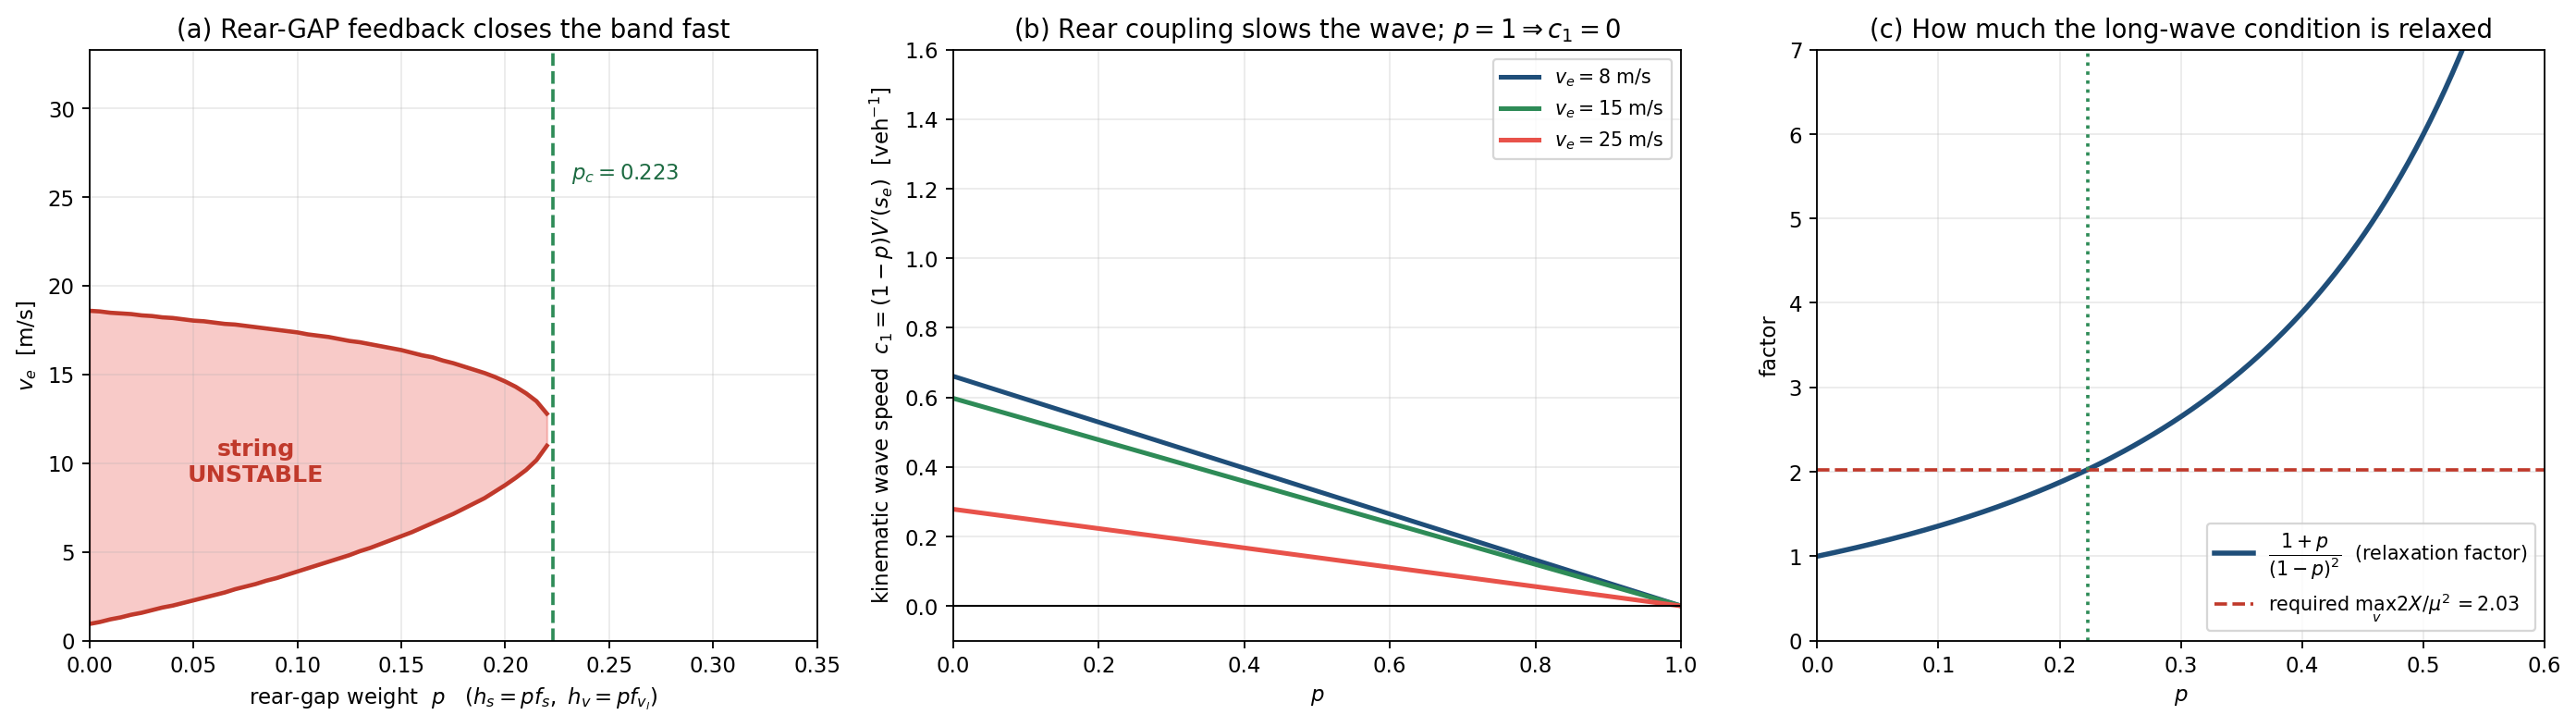
\includegraphics[width=\textwidth]{fig7.png}
\caption{后向间距反馈的稳定带与波速。}
\label{fig:rear-gap-map}
\figurenote{后向间距／相对速度反馈同时改变稳定域和传播速度的三重证据。左图在速度--权重平面扫描长波裕度，原始 IDM 的失稳带随 $p$ 增大从两端收缩，并在 $p_c=0.223$ 完全闭合；这给出“需要多大后视权重”的直接答案。中图绘制 $c_1=(1-p)V'(s_e)$，显示同一反馈在抑制增长的同时降低运动学波速，因而时空轨迹中的色带斜率也应改变。右图分别画出基准模型需要补偿的失稳程度与后视带来的放宽因子，两条曲线的切触／交点复核 $p_c$，避免临界值只来自数值涂色。三图共同证明后向间距反馈不是单纯增加阻尼：它修改了平衡扰动的对流项，因此既决定波会不会增长，也决定波以多快速度传播。}
\end{figure}

\begin{tcolorbox}[notebox,title=\textbf{回到那个疑问}]
文献里"负后视反馈改善稳定性"没有错，第~\ref{sec:multi}~章 的结论也没有错——两者说的根本不是同一个反馈量：
\begin{itemize}[leftmargin=1.2em,itemsep=3pt]
\item \textbf{后向间距／相对速度}反馈进入 $Q,R$，既能改变波速 $c_1$，也能提高稳定裕度；在完全对称极限下可使 $c_1\to0$。本例达到全速域稳定只需 $p\ge0.223$，但波速归零仍要求 $p\to1$；
\item \textbf{后车加速度}反馈只进入 $P$，不改变 $c_1$；它通过零阶矩 $m_0$ 和一阶矩 $m_1$ 调整稳定裕度，取负号时还会降低 $m_0$。
\end{itemize}
所以：\textbf{若论文的后视项作用在间距或速度上，取"负"（$V_B'<0$）确实强烈稳定；若确实是后车加速度项，则单独取负会变差。} 套用结论前，先确认那一项的自变量是什么。
\end{tcolorbox}

\section{数值验证 E9/E10：稳定带闭合与波速下降}
\sectionstudy{experiment}{数值验证 E9/E10：稳定带闭合与波速下降}{wilsonward2011,stuedli2017}

E9 对 $p\in[0,0.4]$ 与 $v_e\in(0,v_0)$ 做二维扫描，记录不稳定带宽；E10 固定 $v_e=8$ m/s、$N=120$，由最低模态相位斜率测波速。

\begin{center}
\small
\captionof{table}{E9/E10 后视稳定带与波速的解析--数值对照。}
\label{tab:e9e10-rear-gap}
\begin{tabular}{p{3.2cm}p{4.3cm}p{4.3cm}p{2.0cm}}
\toprule
\textbf{量} & \textbf{解析预测} & \textbf{数值结果} & \textbf{判定} \\
\midrule
闭合权重 & $p_c=0.223$ & 二维扫描在 $p\approx0.223$ 闭合 & 一致 \\[3pt]
$p=0.223$ 最右根 & 应位于左半平面临界侧 & $-1.2747\times10^{-4}$ s$^{-1}$ & 有限环稳定 \\[3pt]
长波波速 & $(1-p)V'=0.5128$ veh/s & $|\operatorname{Im}\lambda|/k=0.5114$ veh/s & 误差 $0.27\%$ \\
\bottomrule
\end{tabular}
\end{center}
\tabletext{tab:e9e10-rear-gap}{临界权重、有限环最右根和长波波速的解析预测与数值结果。它同时验证了后向间距反馈能够改变稳定裕度和传播速度。}

\begin{tcolorbox}[resultbox,title=\textbf{验证结论}]
后向间距反馈同时完成两件事：把不稳定带从两端向中间收缩，并按 $1-p$ 降低走停波传播速度。有限 $k=2\pi/N$ 下测得的 $0.5114$ veh/s 与长波极限 $0.5128$ veh/s 的小差异属于有限波长修正。这一波速变化可用于实验上区分 S4 与 S2：加速度回望能改增长率，却不改变 $c_1$。
\end{tcolorbox}

\section{具体轨迹结果：后向间距与相对速度反馈}
\sectionstudy{experiment}{具体轨迹结果：后向间距与相对速度反馈}{ngsim2016,thiemann2008,krajewski2018}

图~\ref{fig:traj-s4} 在 $v_e=8$ m/s 比较 $p=0$ 与 $p=0.30>p_c$。加入后视反馈后，$\sigma_v(1800)/\sigma_v(0)$ 从 $48.49$ 降到 $0.00843$，末段斜率为 $-5.16\times10^{-4}$ s$^{-1}$；第 30 辆车速度范围收缩至 $7.9961$--$8.0041$ m/s，间距范围收缩至 $14.0269$--$14.0446$ m。轨迹色带不仅衰减，其传播斜率也与基准不同，对应 $c_1=(1-p)V'$ 的波速降低。

\begin{figure}[htbp]
\centering
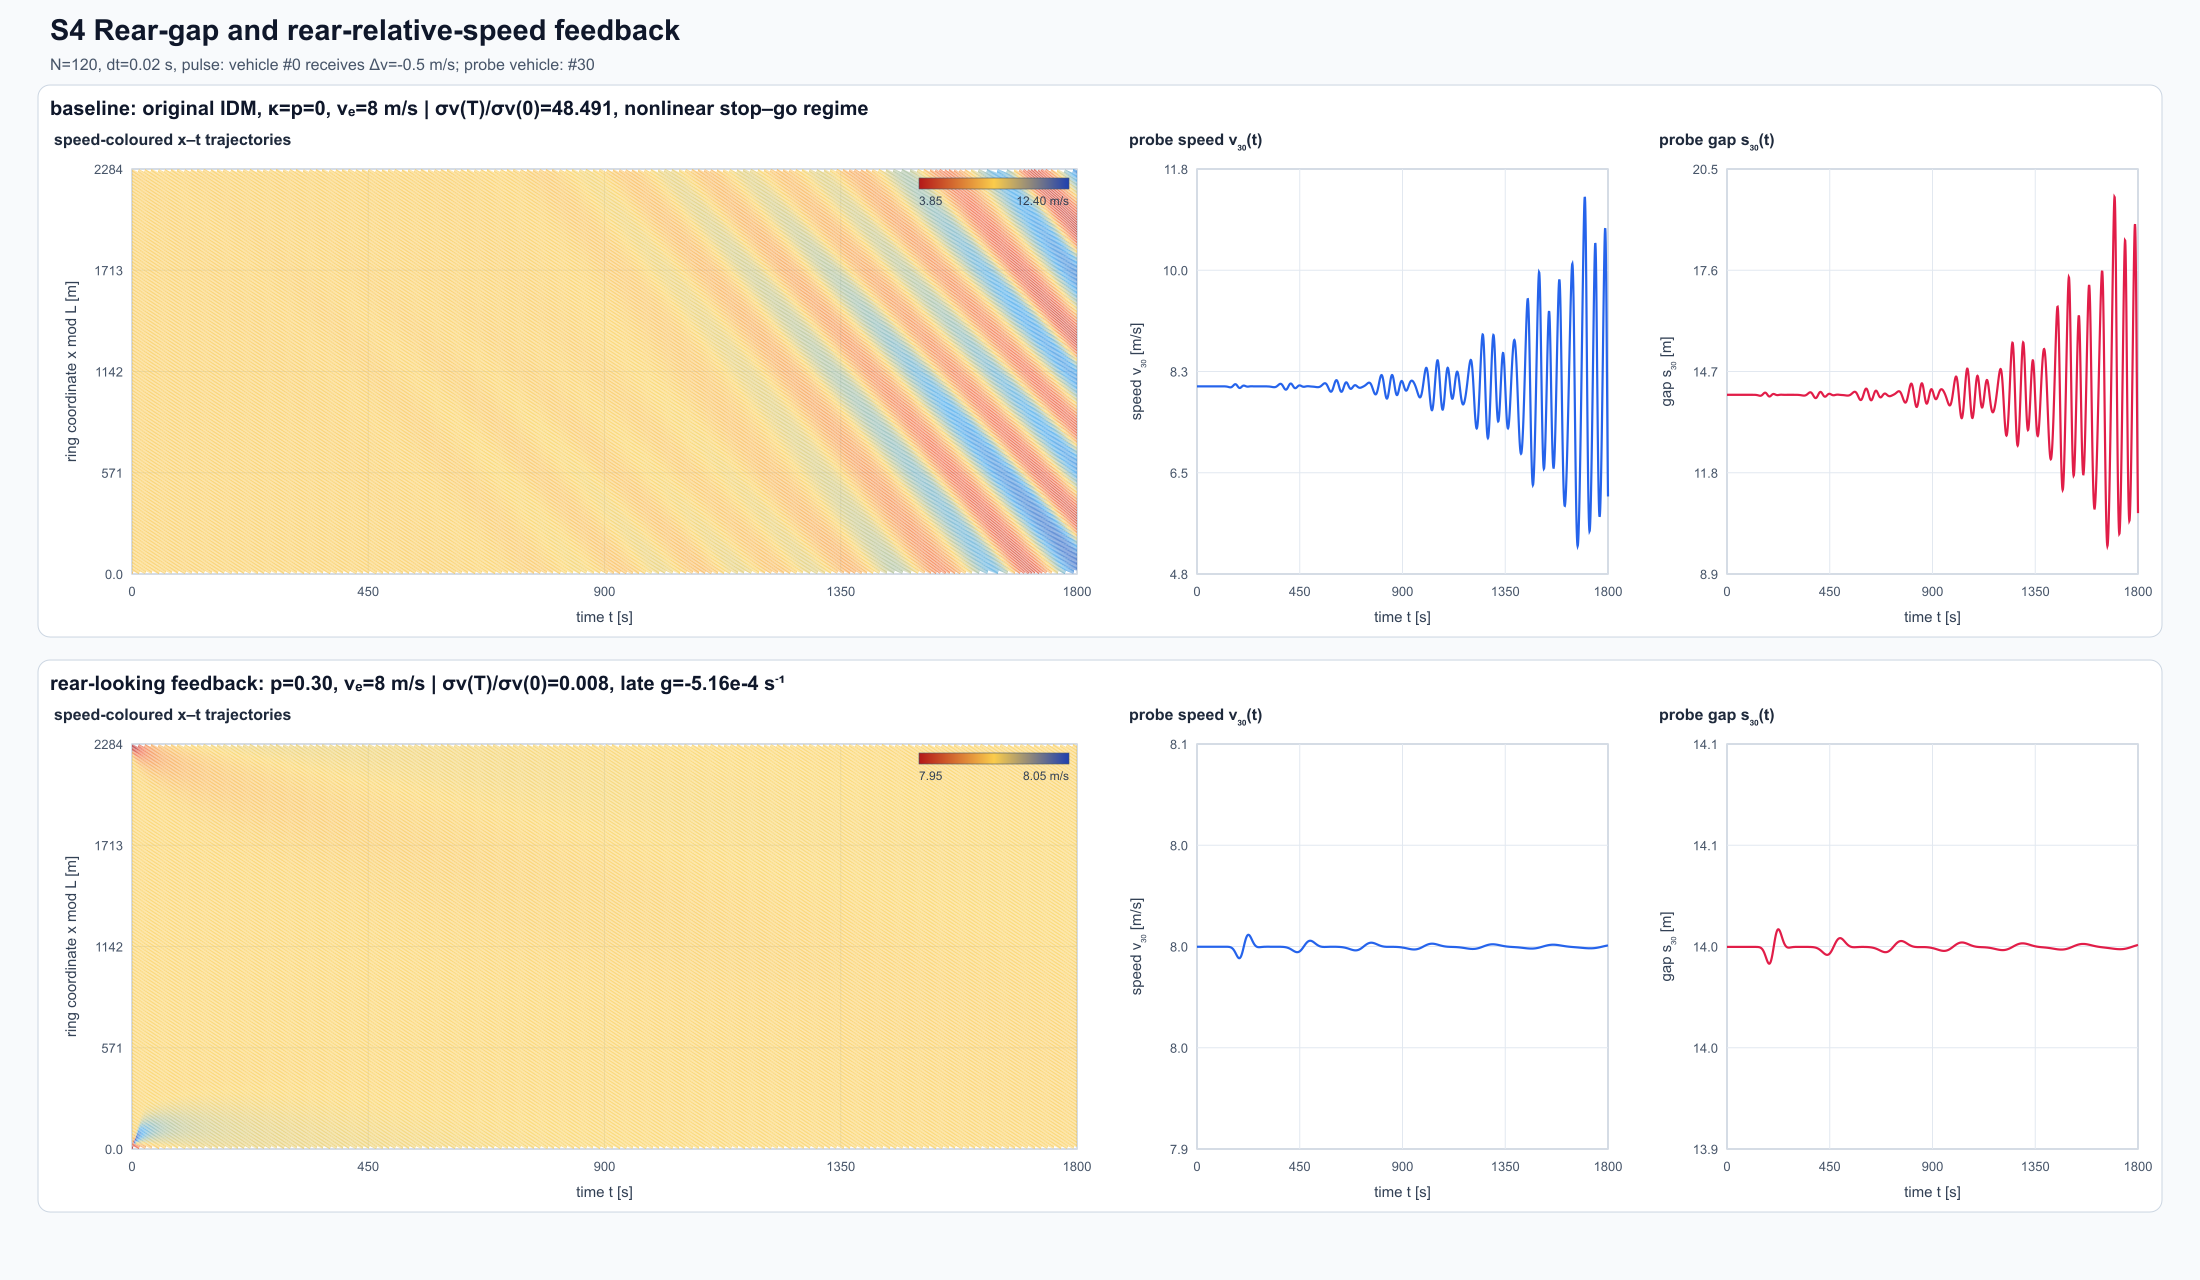
\includegraphics[width=\textwidth]{sim_s4_rear_gap.png}
\caption{S4：后向间距反馈的轨迹对照。}
\label{fig:traj-s4}
\figurenote{S4 对后向间距反馈解析结论的非线性时域验证。上下两行分别取 $p=0$ 和 $p=0.30>p_c$，其余工作点、初始脉冲和色标完全相同；上行形成持续增强的走停波，下行的低速色带在数圈内明显变淡。除了振幅衰减，下行色带在位置--时间平面中的倾角也与上行不同，对应图~\ref{fig:rear-gap-map} 所预测的 $c_1$ 降低；这是一项仅看探针振幅无法得到的证据。右侧探针速度与净间距共同回到平衡，排除了“速度平滑但间距漂移”的伪稳定。该图因此证明后向间距反馈通过改变位置恢复和波速稳定车流，其机制不同于只进入 $\lambda^2$ 系数的后车加速度反馈。}
\end{figure}

%==================================================================
\sectionwrapup{后车加速度反馈与后向间距／相对速度反馈是不同通道：前者主要改变增长率，后者还改变长波传播速度。明确符号约定和反馈变量后，文献中“后视改善稳定性”与前文结论并不矛盾。}

\PART{V}{破坏多项式性：时间延迟}

\chapter{再推广：加速度传递存在时间延迟}
\label{sec:delay}
\chapterguide{延迟为何不改静态门槛，却可能制造新的失稳频段}{本章由拟多项式和含时滞传递函数建立局部与线稳定条件。读者应能区分长波极限、有限频率相位裕度和无限根谱，并知道何时必须由数值求根替代有限维判据。}

\section{模型}
\sectionstudy{model}{模型}{ororsz2004,ororsz2010}

实际中至少有两类延迟：驾驶员（或传感器）的\textbf{感知-反应延迟} $\tau_0$，以及 V2V \textbf{通信延迟} $\tau_a,\tau_b$。分别加到对应的项上：
\begin{equation}
\dot v_n(t) = F\Big(s_n(t-\tau_0),\,v_n(t-\tau_0),\,\dv_n(t-\tau_0)\Big)
+ f_a\,\dot v_{n-1}(t-\tau_a) + f_b\,\dot v_{n+1}(t-\tau_b)
\end{equation}

线性化后：
\begin{equation}
\ddot y_n(t) = f_s\Big(y_{n-1}(t{-}\tau_0)-y_n(t{-}\tau_0)\Big) + f_v\dot y_n(t{-}\tau_0) + f_{v_l}\dot y_{n-1}(t{-}\tau_0)
+ f_a\ddot y_{n-1}(t{-}\tau_a) + f_b\ddot y_{n+1}(t{-}\tau_b)
\end{equation}

\section{特征方程变成超越方程}
\sectionstudy{model}{特征方程变成超越方程}{ororsz2004,ororsz2010}

代入 $y_n=\hat y\,e^{\lambda t+ikn}$，注意时滞对应因子 $e^{-\lambda\tau}$：
\begin{tcolorbox}[keybox]
\begin{equation}
\lambda^2\Big[1 - f_a e^{-\lambda\tau_a - ik} - f_b e^{-\lambda\tau_b + ik}\Big]
- e^{-\lambda\tau_0}\Big[\left(f_v + f_{v_l}e^{-ik}\right)\lambda + f_s\left(e^{-ik}-1\right)\Big] = 0
\end{equation}
\end{tcolorbox}

\begin{tcolorbox}[notebox,title=\textbf{结构性变化}]
这是\textbf{拟多项式}（quasi-polynomial），不再是有限次代数方程，有\textbf{无穷多个根}。Routh--Hurwitz 与 Bilharz 判据\textbf{都不再适用}。可用的手段是：长波展开、频率轴扫描（D-分割）、以及数值伪谱离散。
\end{tcolorbox}

\section{局部稳定性：现在受延迟限制}
\sectionstudy{theory}{局部稳定性：现在受延迟限制}{wilsonward2011,ororsz2010}

冻结前后邻车，加速度耦合项消失，但反应延迟保留：
\begin{equation}
\lambda^2 + e^{-\lambda\tau_0}\left(f_s - f_v\lambda\right) = 0
\end{equation}

令 $\lambda=i\omega$ 求中性边界：
\begin{equation}
e^{-i\omega\tau_0} = \frac{\omega^2}{f_s - i f_v\omega}
\end{equation}

取模得 $\omega^4 = f_s^2+f_v^2\omega^2$，取辐角得 $\omega\tau_0 = \arctan\!\big(\left|f_v\right|\omega/f_s\big)$，于是

\begin{tcolorbox}[keybox,title=\textbf{局部稳定的延迟上限}]
\begin{equation}
\omega_c = \sqrt{\frac{f_v^2 + \sqrt{f_v^4+4f_s^2}}{2}},
\qquad
\tau_0 \;<\; \tau_0^{\rm crit} = \frac{1}{\omega_c}\arctan\!\left(\frac{\left|f_v\right|\omega_c}{f_s}\right)
\end{equation}
\end{tcolorbox}

$\tau_0=0$ 时退化为原来的 $f_v<0,f_s>0$（$\tau_0^{\rm crit}>0$ 恒成立）。对第~\ref{sec:num}~章的 IDM 参数：

\begin{center}
\captionof{table}{三个 IDM 工作点的局部反应延迟上限。}
\label{tab:local-delay-limits}
\begin{tabular}{rccc}
\toprule
$v_e$ [m/s] & 2 & 8 & 20 \\
\midrule
$\omega_c$ [rad/s] & 1.008 & 0.709 & 0.559 \\
$\tau_0^{\rm crit}$ [s] & 1.16 & 1.81 & 2.52 \\
\bottomrule
\end{tabular}
\end{center}
\tabletext{tab:local-delay-limits}{不同平衡速度下的临界频率与局部反应延迟上限。工作点改变恢复刚度与阻尼，因此可容许的延迟不能用一个全速域常数代替。}

\section{长波条件：延迟完全不影响}
\sectionstudy{theory}{长波条件：延迟完全不影响}{ororsz2004,ororsz2010}
\label{sub:delaylw}

这是本节最值得注意的结论。仍令 $\varepsilon=-ik$、$\lambda=c_1\varepsilon+c_2\varepsilon^2+\cdots$。由于 $\lambda=O(\varepsilon)$，
\begin{equation}
e^{-\lambda\tau} = 1 - c_1\tau\,\varepsilon + O(\varepsilon^2)
\end{equation}

把方程写成 $\lambda^2 M = e^{-\lambda\tau_0}N$，其中
\begin{equation}
N = \left(f_v+f_{v_l}e^{\varepsilon}\right)\lambda + f_s\left(e^{\varepsilon}-1\right)
= \underbrace{\left[\left(f_v+f_{v_l}\right)c_1+f_s\right]}_{\textstyle =\,0}\varepsilon
+ \left[\left(f_v+f_{v_l}\right)c_2 + f_{v_l}c_1 + \frac{f_s}{2}\right]\varepsilon^2 + O(\varepsilon^3)
\end{equation}

\begin{tcolorbox}[notebox,title=\textbf{关键的一步}]
$e^{-\lambda\tau_0}$ 的一阶修正 $-c_1\tau_0\varepsilon$ 要乘上 $N$ 的 $O(\varepsilon)$ 系数才能贡献到 $O(\varepsilon^2)$——\textbf{而那个系数恰好为零}（它正是定出 $c_1$ 的方程）。所以 $\tau_0$ 在 $O(\varepsilon^2)$ 阶被完全"吃掉"。同理 $M$ 中的延迟修正是 $O(\varepsilon)$，乘上 $\lambda^2=O(\varepsilon^2)$ 只到 $O(\varepsilon^3)$。
\end{tcolorbox}

于是 $c_1=V'(s_e)$ 与
\begin{equation}
\left(1-f_a-f_b\right)c_1^2 = \frac{f_s}{2} + f_{v_l}c_1 + \left(f_v+f_{v_l}\right)c_2
\end{equation}
都与无延迟时\textbf{逐字相同}：

\begin{tcolorbox}[keybox,title=\textbf{长波条件（含任意延迟）}]
\begin{equation}
\frac{1}{2}\left(f_v^2-f_{v_l}^2\right) \;\ge\; \left(1-f_a-f_b\right)f_s
\end{equation}
\textbf{与 $\tau_0,\tau_a,\tau_b$ 全部无关。}
\end{tcolorbox}

物理上很直白：$k\to0$ 意味着 $\lambda\to0$，即扰动变化极慢，延迟环节 $e^{-\lambda\tau}\to1$，相位滞后可以忽略。\textbf{延迟的破坏作用只在有限频率上体现}——这与第~\ref{sec:lead}~章 $f_a>1$ 的情形是同一类现象。

\section{有限频率条件：单向情形的精确判据}
\sectionstudy{theory}{有限频率条件：单向情形的精确判据}{ororsz2004,ororsz2010}

对单向模型（$f_b=0$），Laplace 变换后仍可分离出传递函数：
\begin{tcolorbox}[keybox]
\begin{equation}
G(\lambda) = \frac{e^{-\lambda\tau_0}\left(f_s+f_{v_l}\lambda\right) + f_a\lambda^2 e^{-\lambda\tau_a}}
{\lambda^2 + e^{-\lambda\tau_0}\left(f_s - f_v\lambda\right)}
\end{equation}
\end{tcolorbox}

它不再是有理函数，但\textbf{判据形式不变}：$\left\|G\right\|_\infty\le1$，且分母在右半平面无零点（即 $\tau_0<\tau_0^{\rm crit}$）。

代入 $\lambda=i\omega$，记 $\theta_0=\omega\tau_0$、$\phi=\omega(\tau_a-\tau_0)$。利用 $\left|e^{-i\theta}\right|=1$：
\begin{align}
\left|N\right|^2 &= f_s^2+f_{v_l}^2\omega^2 + f_a^2\omega^4
- 2f_a\omega^2\left[f_s\cos\phi - f_{v_l}\omega\sin\phi\right] \\
\left|D\right|^2 &= \omega^4 + f_s^2 + f_v^2\omega^2
- 2\omega^2\left[f_s\cos\theta_0 - f_v\omega\sin\theta_0\right]
\end{align}

作差、约去公因子 $\omega^2$：

\begin{tcolorbox}[keybox,title=\textbf{含延迟的线稳定性判据}]
\begin{align}
\Psi(\omega) = \;& \left(1-f_a^2\right)\omega^2 + f_v^2 - f_{v_l}^2 \nonumber\\
& - 2f_s\cos\!\left(\omega\tau_0\right) + 2f_v\,\omega\sin\!\left(\omega\tau_0\right) \nonumber\\
& + 2f_af_s\cos\!\left(\omega(\tau_a{-}\tau_0)\right) - 2f_af_{v_l}\,\omega\sin\!\left(\omega(\tau_a{-}\tau_0)\right)
\;\ge\; 0
\qquad \forall\,\omega\ge0
\label{eq:Psi}
\end{align}
\end{tcolorbox}

\textbf{一致性检验.} 令 $\tau_0=\tau_a=0$，式~\eqref{eq:Psi} 退化为 $(1-f_a^2)\omega^2+f_v^2-f_{v_l}^2-2f_s(1-f_a)$，即第~\ref{sec:lead}~章的 $H(u)$。而
\begin{equation}
\Psi(0) = f_v^2 - f_{v_l}^2 - 2f_s\left(1-f_a\right)
\end{equation}
——\textbf{恰是长波条件，且不含任何延迟}，与 \S\ref{sub:delaylw} 一致。

\section{小 \texorpdfstring{$\omega$}{omega} 展开：延迟如何产生有限频率负裕度}
\sectionstudy{theory}{小 \texorpdfstring{$\omega$}{omega} 展开：延迟如何产生有限频率负裕度}{ororsz2004,ororsz2010}

$\Psi$ 是 $\omega$ 的偶函数，展开到 $\omega^2$：
\begin{equation}
\Psi(\omega) \approx \Psi(0) + \Lambda\,\omega^2,
\qquad
\boxed{\;\Lambda = \left(1-f_a^2\right) + f_s\tau_0^2 + 2f_v\tau_0
- f_af_s\left(\tau_a{-}\tau_0\right)^2 - 2f_af_{v_l}\left(\tau_a{-}\tau_0\right)\;}
\end{equation}

因 $f_v<0$，项 $2f_v\tau_0$ \textbf{恒为负}：反应延迟直接压低 $\Lambda$。当 $\Lambda<0$ 时 $\Psi$ 在 $\omega=0$ 右侧下凹形成"势阱"；阱底一旦触零，就出现\textbf{有限波长}的线不稳定。

因此实用上有一个两级判据：
\begin{itemize}[leftmargin=1.4em,itemsep=3pt]
\item $\Psi(0)\ge0$：长波条件，必要，与延迟无关；
\item $\Lambda\ge0$：保证 $\Psi$ 单调上升、不出现势阱，是\textbf{充分}的保险条件（但偏保守，因为 $\Psi(0)>0$ 时允许一定深度的阱）。
\end{itemize}

\section{校验：带反应延迟的 OVM}
\sectionstudy{theory}{校验：带反应延迟的 OVM}{bando1995,jiang2001}

$\dot v = \left[V(s)-v\right]/\tau$ 有 $f_s=aV'$、$f_v=-a$、$f_{v_l}=0$（$a=1/\tau$），故
\begin{equation}
\Psi(\omega) = \omega^2 + a^2 - 2aV'\cos\!\left(\omega\tau_0\right) - 2a\,\omega\sin\!\left(\omega\tau_0\right)
\end{equation}
\begin{itemize}[leftmargin=1.4em,itemsep=3pt]
\item $\Psi(0)=a^2-2aV'\ge0 \iff V'\le a/2$，与经典无延迟结果一致；
\item $\Lambda = 1 + aV'\tau_0^2 - 2a\tau_0$。取 $a=1$、$V'=0.4$：$\Lambda<0$ 始于 $\tau_0=0.564$ s，而 $\Psi$ 真正触零在 $\tau_0\approx0.81$ s，局部稳定上限为 $\tau_0^{\rm crit}=1.14$ s。三个数依次出现，印证了上面"两级判据"的保守性排序。
\end{itemize}

\section{数值算例：IDM}
\sectionstudy{experiment}{数值算例：IDM}{treiber2000,treiberkesting2013}

\textbf{(1) 反应延迟拓宽不稳定带（$f_a=0$）.}

\begin{center}
\captionof{table}{反应延迟引起的 IDM 不稳定带扩张。}
\label{tab:reaction-delay-band}
\begin{tabular}{rcc}
\toprule
$\tau_0$ [s] & 不稳定速度带 [m/s] & 带宽 \\
\midrule
0.00 & $0.93$ -- $18.59$ & 17.66 \\
0.50 & $0$ -- $18.59$ & 18.59 \\
1.00 & $0$ -- $19.75$ & 19.75 \\
1.25 & $0$ -- $23.71$ & 23.71 \\
1.50 & $0$ -- $25.98$ & 25.98 \\
\bottomrule
\end{tabular}
\end{center}
\tabletext{tab:reaction-delay-band}{反应延迟由 0 增至 1.5 s 时不稳定速度带的变化。延迟先吞没低速稳定区，随后通过有限频率负裕度推高上边界。}

注意上边界 $18.59$ m/s 在 $\tau_0\lesssim0.9$ s 内\textbf{纹丝不动}——因为该边界由 $\Psi(0)=0$ 决定，与延迟无关。延迟先是从下方吞掉低速稳定区，之后才在有限频率上把上边界推高。

\textbf{(2) 通信延迟压缩可用增益窗口.} 取 $\tau_0=0$、$f_a=\kappa$，要求全速域线稳定：

\begin{center}
\captionof{table}{通信延迟对可行前馈增益窗口的压缩。}
\label{tab:communication-delay-window}
\begin{tabular}{rcc}
\toprule
$\tau_a$ [s] & 可行 $\kappa$ 下界 & 可行 $\kappa$ 上界 \\
\midrule
0.0 & 0.134 & 1.00 \\
0.5 & 0.134 & 0.82 \\
1.0 & 0.134 & 0.69 \\
1.5 & 0.134 & 0.60 \\
\bottomrule
\end{tabular}
\end{center}
\tabletext{tab:communication-delay-window}{通信延迟变化时 $\kappa$ 的稳定下界和上界。长波下界始终为 0.134，而有限频率上界持续下降，清楚区分了静态门槛与相位裕度。}

\textbf{下界恒为 $\kappa_c=0.134$}（长波阈值，延迟无关），上界随延迟单调下降。

\begin{figure}[htbp]
\centering
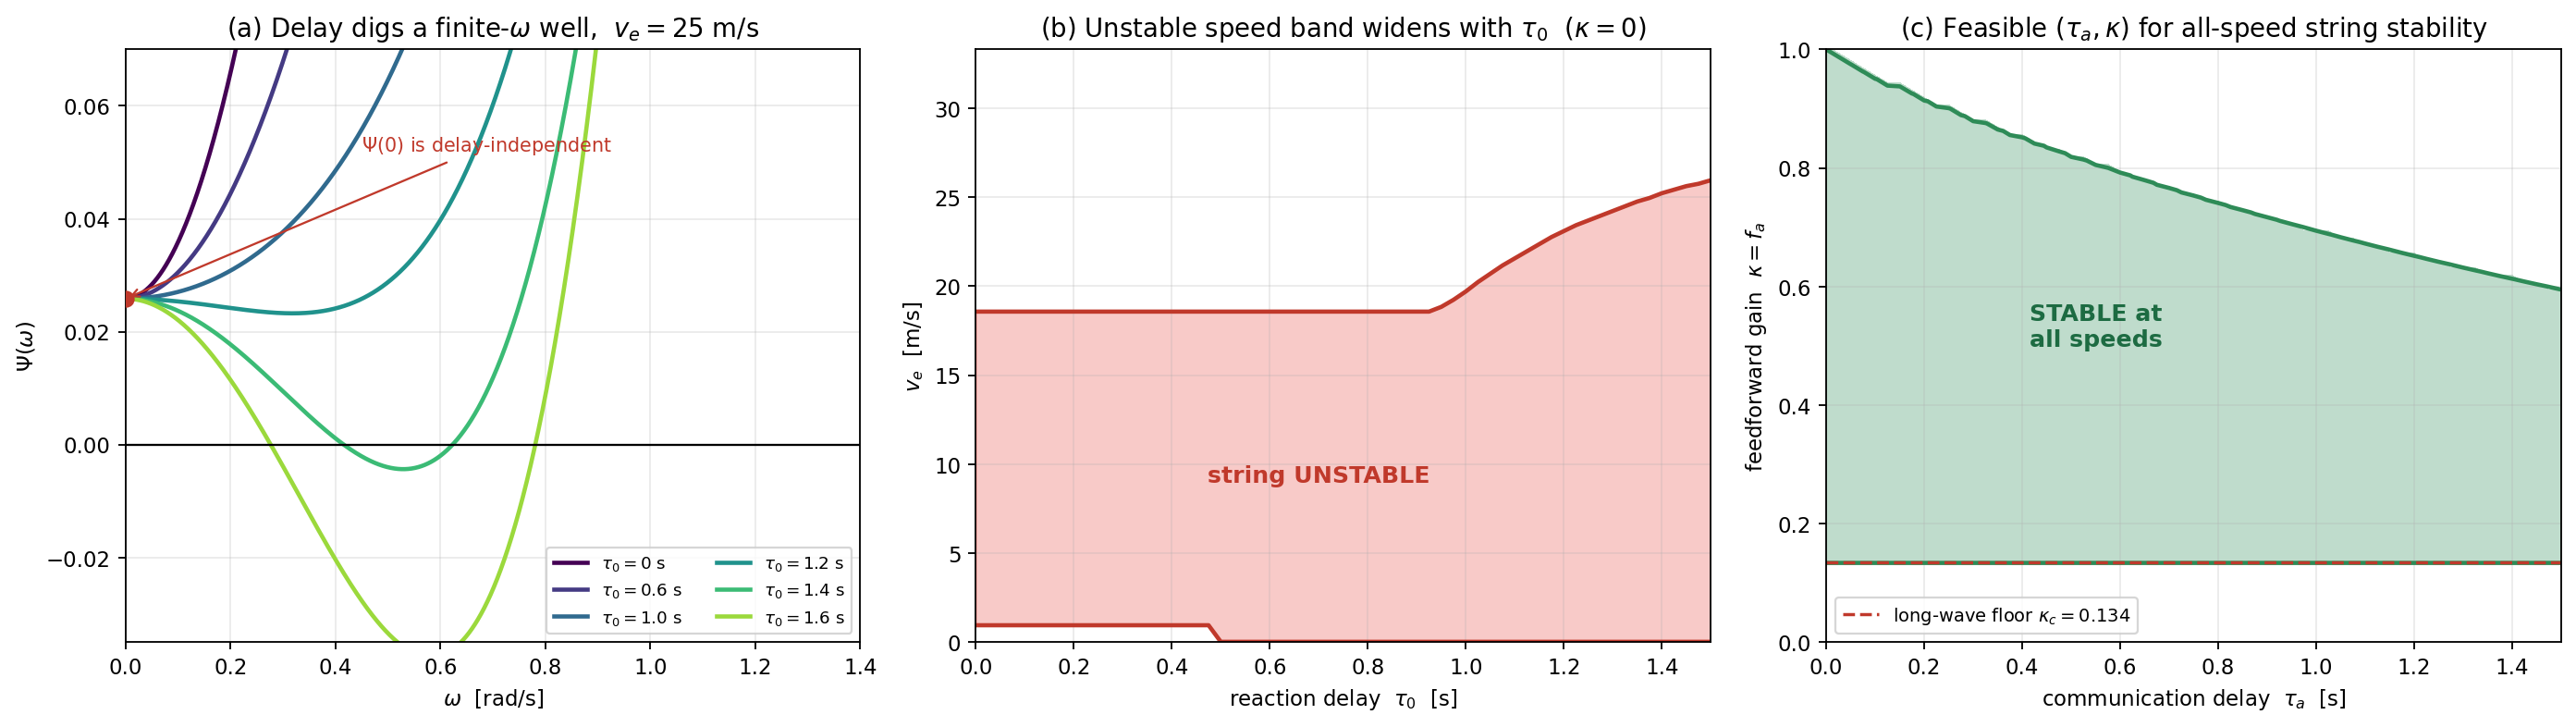
\includegraphics[width=\textwidth]{fig4.png}
\caption{反应与通信延迟的稳定性影响。}
\label{fig:delay-map}
\figurenote{反应延迟和通信延迟如何从有限频率方向侵蚀稳定性。左图在 $v_e=25$ m/s 比较不同反应延迟的频域裕度 $\Psi(\omega)$：所有曲线在 $\omega=0$ 具有相同起点，验证延迟因子在零频率等于 1；但随着延迟增大，有限频率处的谷值下沉并穿过零线，产生长波展开看不到的新失稳分支。中图把每个延迟的最坏频率结果投影到速度轴，可见低速稳定区首先被吞没，随后整个不稳定带扩张。右图给出通信延迟与前馈增益的可行域：稳定下界基本不动，而高增益上界持续下降，说明延迟把原本有利的强反馈变成相位滞后的风险。三图证明“延迟不影响长波门槛”不等于“延迟不影响稳定性”，任何含延迟设计都必须检查完整频率区间。}
\end{figure}

\section{双向耦合与延迟}
\sectionstudy{theory}{双向耦合与延迟}{ororsz2004,ororsz2010}

$f_b\ne0$ 时标量逐车传递函数不再适用（\S\ref{sub:nofail}），而拟多项式又使有限维 Bilharz 闭式不再适用。此时可采用：
\begin{itemize}[leftmargin=1.4em,itemsep=3pt]
\item 长波条件仍有闭式，且仍与延迟无关：$\tfrac12(f_v^2-f_{v_l}^2)\ge(1-f_a-f_b)f_s$；
\item 有限波长部分做\textbf{数值处理}：对每个 $k$ 用 D-分割法在 $\lambda=i\omega$ 上扫描中性边界，或用伪谱配点法离散时滞算子求最右特征值。
\end{itemize}

\begin{tcolorbox}[notebox,title=\textbf{工程结论}]
\begin{itemize}[leftmargin=1.2em,itemsep=3pt]
\item \textbf{延迟不改变长波门槛。} 要不要加前馈、加多少才够，这个"底线"完全由静态偏导决定，标定时不必担心延迟。
\item \textbf{延迟的代价体现在增益上限。} 通信延迟每增加约 0.5 s，本例可用 $\kappa$ 的上界下降约 $0.1$--$0.2$。高增益 $+$ 大延迟是危险组合。
\item \textbf{反应延迟通常比通信延迟更不利。} $\tau_0$ 同时作用于 $f_s,f_v,f_{v_l}$ 三项，并在 $\Lambda$ 中贡献恒负的一阶项 $2f_v\tau_0$；通信延迟只作用于前馈项，且以 $(\tau_a-\tau_0)$ 的形式出现。当两者接近时，部分相位效应可能相互抵消。
\item 由此还有一条反直觉的设计提示：\textbf{人为把前馈信号延迟到与感知延迟同步}（$\tau_a\approx\tau_0$）反而比"尽量快"更稳，因为 $\Lambda$ 中的 $-2f_af_{v_l}(\tau_a-\tau_0)$ 项在 $\tau_a<\tau_0$ 时为正、$\tau_a>\tau_0$ 时为负。
\end{itemize}
\end{tcolorbox}

\section{数值验证 E8：长波门槛不动，有限频率势阱下沉}
\sectionstudy{experiment}{数值验证 E8：长波门槛不动，有限频率势阱下沉}{ororsz2004,ororsz2010}

实验分两层。第一层只计算 $\Psi(0)$，检查不同延迟下长波门槛是否保持不变；第二层在 $\omega\in[0,6]$ rad/s 上细扫 $\Psi(\omega)$，以 $\min_\omega\Psi=0$ 定位有限频率失稳。最后用带历史缓冲的时域仿真复核稳定符号。

\begin{center}
\small
\captionof{table}{E8 延迟扫描中的不变量与有限频率结果。}
\label{tab:e8-delay-validation}
\begin{tabular}{p{3.2cm}p{3.4cm}p{3.7cm}p{3.2cm}}
\toprule
\textbf{扫描} & \textbf{不变量} & \textbf{有限频率结果} & \textbf{解释} \\
\midrule
$\tau_0:0\to0.5$ s & 上边界 $18.59$ m/s 不动 & 下边界由 $0.93$ 降到 $0$ & 低速稳定区先被吞没 \\[3pt]
$\tau_0=1.5$ s & 长波公式仍不含 $\tau_0$ & 不稳定带扩为 $0$--$25.98$ m/s & 势阱继续下沉并展宽 \\[3pt]
$\tau_a:0\to1.5$ s & $\kappa$ 下界恒为 $0.134$ & 上界由 $1.00$ 降到 $0.60$ & 通信延迟压缩增益窗口 \\
\bottomrule
\end{tabular}
\end{center}
\tabletext{tab:e8-delay-validation}{反应延迟和通信延迟扫描中保持不变的长波门槛，以及随延迟变化的有限频率失稳结果。该表说明“长波条件不变”不等于“整个系统稳定域不变”。}

\begin{tcolorbox}[resultbox,title=\textbf{验证结论}]
所有 $\Psi(\omega)$ 曲线从同一个 $\Psi(0)$ 出发，但在正频率处随延迟下沉。因而“长波条件满足”只是必要条件：当 $\Psi(0)\ge0$ 而 $\min_{\omega>0}\Psi<0$ 时，仿真仍会出现有限波长增长。该实验直接验证了延迟为何不改最低所需前馈量，却会降低允许的最高增益。
\end{tcolorbox}

\section{具体轨迹结果：反应延迟诱发走停波}
\sectionstudy{experiment}{具体轨迹结果：反应延迟诱发走停波}{ororsz2004,ororsz2010}

图~\ref{fig:traj-s5} 固定 $v_e=19$ m/s。无延迟时 $\sigma_v(1800)/\sigma_v(0)=0.0106$；仅加入 $\tau_0=1.10$ s 后，该比值升至 $165.68$，并进入有限振幅走停波。探针车速度扩展到 $0$--$26.01$ m/s，间距扩展到 $3.04$--$60.26$ m。最小间距仍为正，因此图中强振荡不是车辆穿透造成的数值伪影。该算例说明：即使无延迟的高速度工作点稳定，有限频率势阱也可被反应延迟推入失稳区。

\begin{figure}[htbp]
\centering
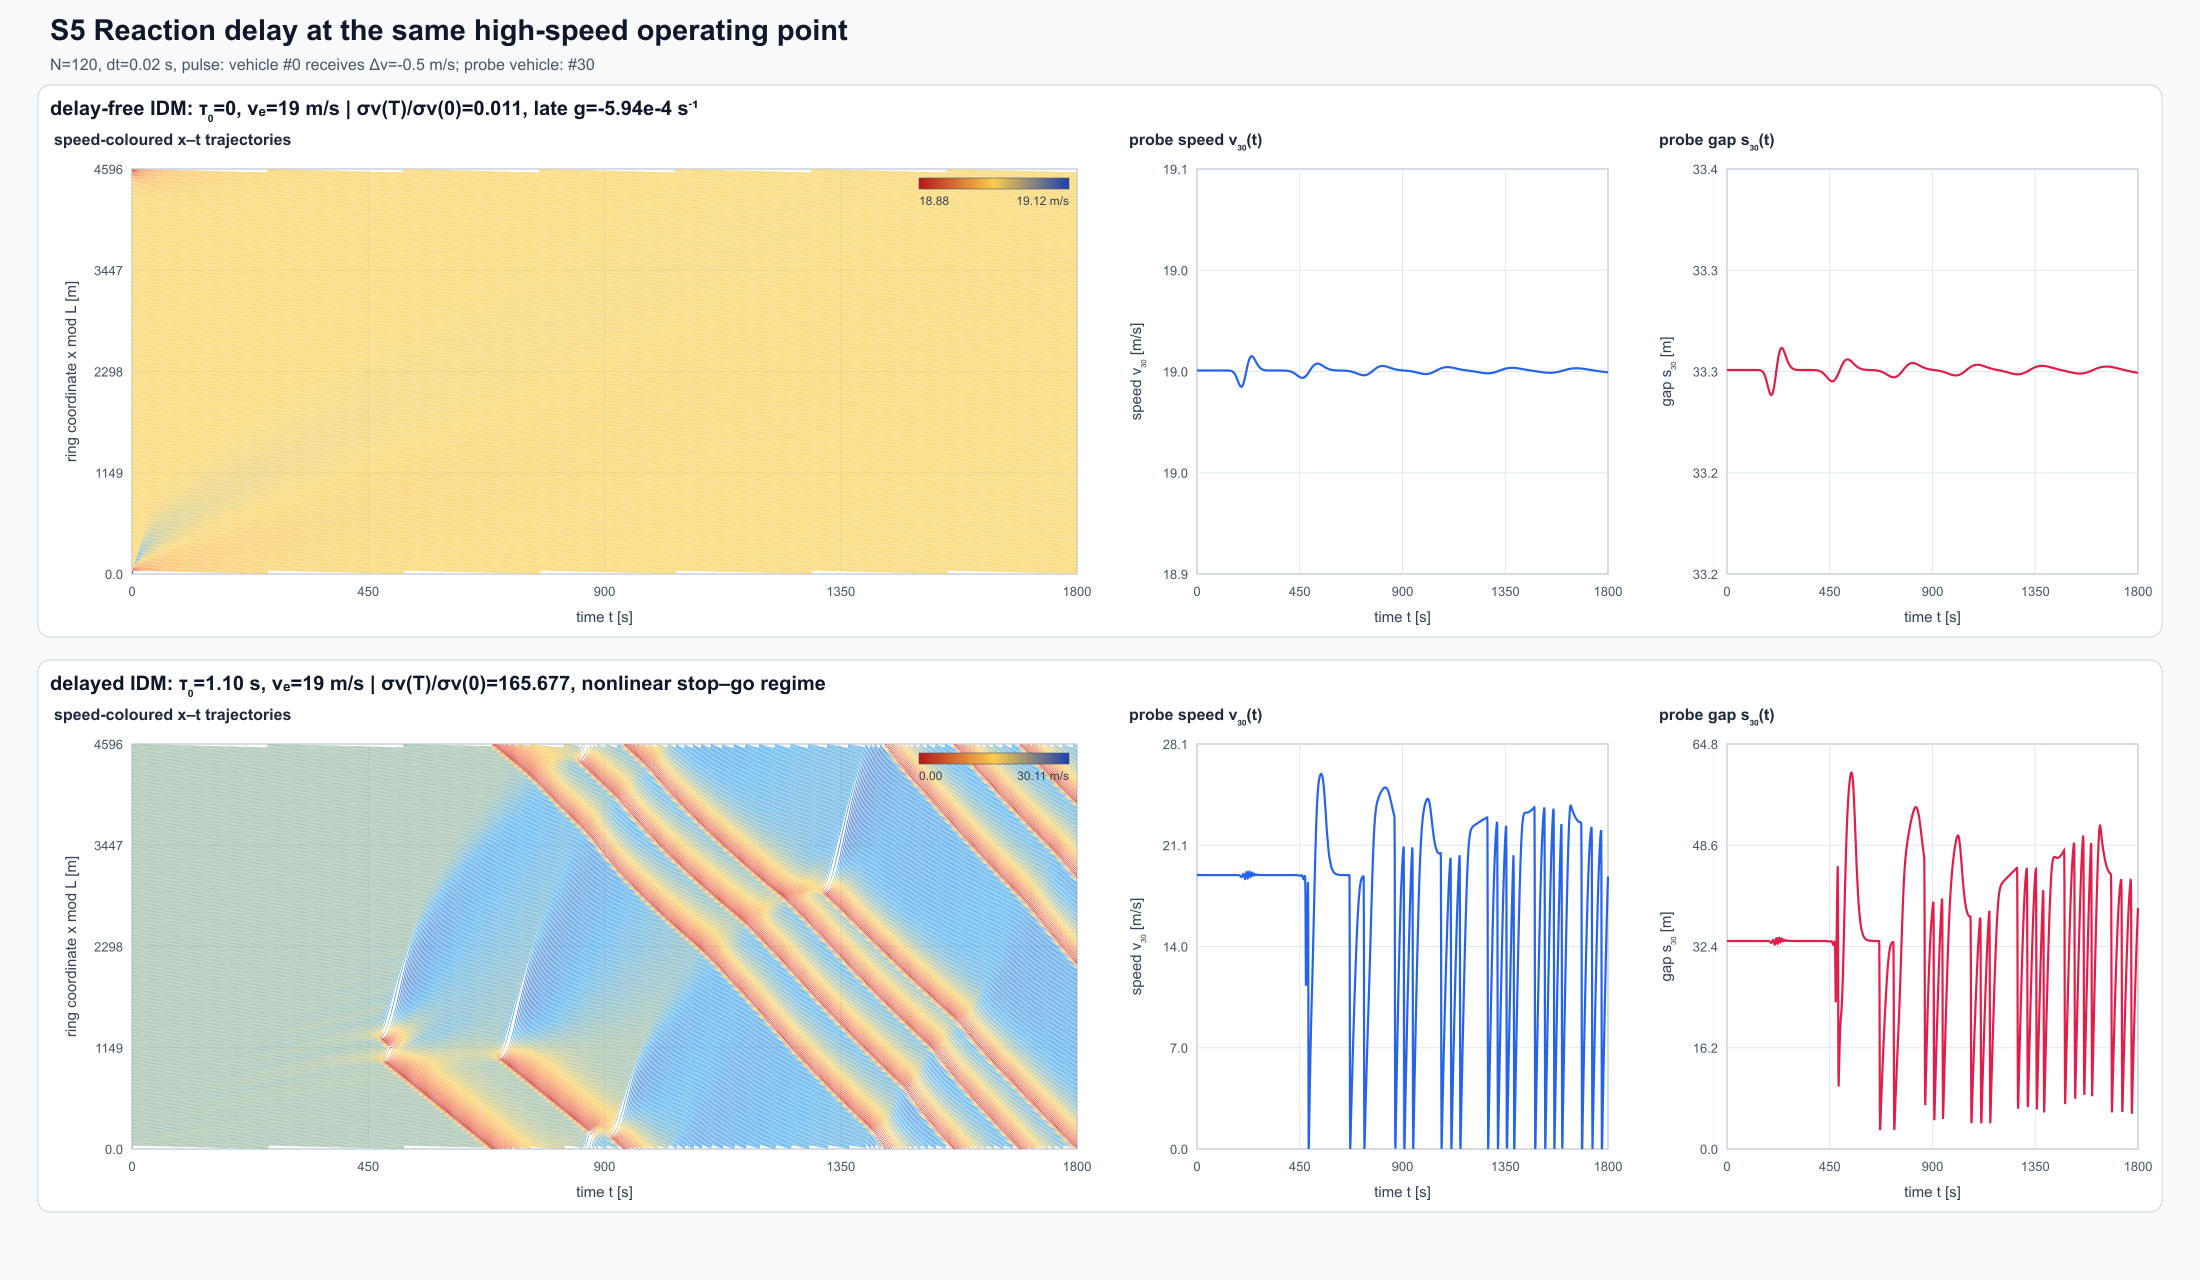
\includegraphics[width=\textwidth]{sim_s5_delay.png}
\caption{S5：反应延迟诱发的走停波。}
\label{fig:traj-s5}
\figurenote{S5 将图~\ref{fig:delay-map} 中的有限频率负裕度转化为实际走停波。两行均取靠近原始稳定边界的 $v_e=19$ m/s，只把反应延迟由零改为 1.10 s，因而差异不能归因于密度或初始扰动。无延迟行的色带在上游传播时逐渐变淡，探针速度和间距收敛；延迟行则出现多条色带相互追赶、合并并加深，第 30 辆车反复进入低速状态，同时产生大幅间距压缩与释放。波形不是最长的单一正弦，而具有由危险有限频率选择出来的较短时空尺度，这正是只看 $\omega\to0$ 会漏判的现象。该图证明 1.10 s 延迟可以把解析上原本稳定的工作点推入非线性走停波状态，并说明通信／感知时延必须与增益共同设计。}
\end{figure}

%==================================================================
\sectionwrapup{反应和通信延迟把特征多项式变为拟多项式，引入无限多个根。长波静态门槛可能不变，但有限频率相位裕度会显著缩小；因此必须在目标增益之外扫描延迟谱，并用时域仿真验证最危险根。}

\PART{VI}{破坏均匀性：异质车队与混合交通}

%==================================================================
\chapter{异质车队：\texorpdfstring{$F_n\ne F_{n-1}$}{车辆模型不同}}
\label{sec:het}
\chapterguide{车型配方相同，排列不同为何仍会产生不同传播结果}{本章在 Fourier 对角化失效后转向逐车传递函数的链式乘积，建立加权前缀和、排序效应和 AV 相邻对规则，并把渗透率--速度二维稳定域用于混合交通设计。}

前面各章都假设车队均匀。实际车流中车型、驾驶风格、是否装备 ACC／CACC 各不相同，即每辆车有自己的 $F_n$。本章给出相应的分析框架。

\section{平衡态不再均匀}
\sectionstudy{model}{平衡态不再均匀}{talebpour2016,feng2019,stern2018}

平衡要求所有车\textbf{速度相同}（否则间距会持续变化），但\textbf{间距各不相同}：
\begin{equation}
v_e^{(n)} = v_e \ \ \forall n,
\qquad
s_e^{(n)} = V_n^{-1}(v_e)
\end{equation}
基本图上的密度改用平均间距 $\bar s_e(v_e)=\frac{1}{N}\sum_n s_e^{(n)}$，即
$\rho = 1/\left(\bar s_e + \bar l\right)$。

每辆车在自己的平衡点处有各自的偏导 $f_s^{(n)},f_v^{(n)},f_{v_l}^{(n)}$，线性化方程为
\begin{equation}
\ddot y_n = f_s^{(n)}\left(y_{n-1}-y_n\right) + f_v^{(n)}\dot y_n + f_{v_l}^{(n)}\dot y_{n-1}
\end{equation}

\section{结构性变化：平移不变性丧失}
\sectionstudy{theory}{结构性变化：平移不变性丧失}{talebpour2016,feng2019,stern2018}

\begin{tcolorbox}[notebox,title=\textbf{Fourier 模态失效}]
系数随 $n$ 变化，矩阵 $A,B$ \textbf{不再是循环矩阵}，DFT 基不再对角化它们（对照 \S\ref{sub:circulant}）。空间 Fourier 分析在异质车队中\textbf{根本不适用}。

但\textbf{单向级联结构仍在}：$y_n$ 只依赖 $y_{n-1}$。所以传递函数方法\textbf{反而是这里唯一好用的工具}——与双向耦合的情形正好相反。
\end{tcolorbox}

\section{逐车传递函数与链式乘积}
\sectionstudy{theory}{逐车传递函数与链式乘积}{swaroop1996,ploeg2014,feng2019}

对第 $n$ 辆车单独作 Laplace 变换：
\begin{tcolorbox}[keybox]
\begin{equation}
G_n(\lambda) = \frac{\hat y_n}{\hat y_{n-1}}
= \frac{f_s^{(n)} + f_{v_l}^{(n)}\lambda + f_a^{(n)}\lambda^2}{\lambda^2 - f_v^{(n)}\lambda + f_s^{(n)}}
\end{equation}
（$f_a^{(n)}$ 为该车的前车加速度前馈增益，无前馈时取 $0$。）扰动从第 $0$ 辆传到第 $j$ 辆的增益为\textbf{连乘}：
\begin{equation}
\frac{\hat y_j}{\hat y_0} = \prod_{n=1}^{j} G_n(\lambda)
\end{equation}
\end{tcolorbox}

\section{三级判据}
\sectionstudy{theory}{三级判据}{talebpour2016,feng2019,stern2018}

\begin{table}[htbp]
\centering
\small
\caption{异质单向车队的三级稳定性判据。}
\label{tab:heter-three-levels}
\begin{tabular}{p{2.6cm}p{5.4cm}p{5.8cm}}
\toprule
& \textbf{条件} & \textbf{含义} \\
\midrule
(i) 局部稳定 & $f_s^{(n)}>0$，$f_v^{(n)}<0$，逐车 & 每辆车自身不发散 \\[4pt]
(ii) \textbf{严格}线稳定 & $\left\|G_n\right\|_\infty\le1$，逐车 & 最强；与车队组成、排序\textbf{完全无关}，任意混合都安全 \\[10pt]
(iii) \textbf{车队}线稳定 & $\max\limits_\omega\left|\prod_{n\le j}G_n(i\omega)\right|\le1$，$\forall j$ & 允许个别车放大，只要被前后的衰减车抵消；\textbf{依赖排序} \\
\bottomrule
\end{tabular}
\end{table}

表~\ref{tab:heter-three-levels} 给出了由“单车不发散”到“任意前缀不放大”的三个层级。条件 (ii) 最强但也最保守，实际车流中几乎没有一辆人类驾驶车能满足；工程上通常使用条件 (iii)，允许局部放大由后续稳定车辆抵消，但必须保留排序信息。

\section{环道：闭合方程、频域充分条件与前缀放大不是一回事}
\sectionstudy{model}{环道：闭合方程、频域充分条件与前缀放大不是一回事}{talebpour2016,feng2019,stern2018}

\subsection{闭合方程不是对任意 $\lambda$ 成立的恒等式}

记一整圈的开环传递函数为
\[
H(\lambda):=\prod_{n=1}^{N}G_n(\lambda).
\]
从参考车辆 $0$ 出发逐车传递一圈，有 $\hat y_N=H(\lambda)\hat y_0$；环道闭合又要求 $\hat y_N=\hat y_0$。对非零模态 $\hat y_0\ne0$，因此得到
\begin{tcolorbox}[keybox,title=\textbf{环道特征方程}]
\begin{equation}
\prod_{n=1}^{N} G_n(\lambda) = 1.
\label{eq:heter-ring-closure}
\end{equation}
\end{tcolorbox}
式~\eqref{eq:heter-ring-closure} 的含义是“\textbf{寻找哪些特殊的 $\lambda$ 能使乘积等于 1}”，而不是说乘积对任意 $\lambda$ 恒等于 1。这与 $\det(\lambda I-A)=0$ 是求特征值方程、而非恒等式完全相同。均匀时它退化为 $G(\lambda)^N=1$，其 $N$ 个可能相位为
\[
G(\lambda)=\exp\!\left(i\frac{2\pi m}{N}\right)=e^{ik_m},
\qquad k_m=\frac{2\pi m}{N},\quad m=0,\ldots,N-1,
\]
正是 第~\ref{sec:appx}~章 的离散波数。$\lambda=0$ 时各车同量平移，间距与速度均不变；这是平移对称产生的中性模态，判断交通扰动稳定时应单独排除。

\subsection{为什么闭合方程之外还要检查 $|H(i\omega)|$}

精确判定环道稳定性，应求式~\eqref{eq:heter-ring-closure} 的全部根，并检查除平移根外是否均有 $\operatorname{Re}\lambda<0$。为避免直接求复杂超越方程，可在稳定区域边界 $\lambda=i\omega$ 上使用一个更容易计算的充分条件：

\begin{tcolorbox}[keybox,title=\textbf{环道的模长充分条件}]
\begin{equation}
\left|H(i\omega)\right|
=\prod_{n=1}^{N}\left|G_n(i\omega)\right| \le 1
\quad \forall\omega
\qquad\Longrightarrow\qquad \text{环道不产生增长模态}.
\label{eq:heter-ring-gain}
\end{equation}
\end{tcolorbox}

两式并不矛盾。$H(\lambda)=1$ 只在\textbf{特征值}处成立；式~\eqref{eq:heter-ring-gain} 则把 $\lambda=i\omega$ 当作连续试探点，检查整条虚轴上的开环增益。复数真正等于 1 必须同时满足
\[
|H(i\omega)|=1,
\qquad
\arg H(i\omega)=2\pi q.
\]
若 $|H(i\omega)|<1$，它当然不可能等于 1。在每辆车局部稳定、因而 $H$ 在右半平面解析且高频有界的前提下，最大模原理把虚轴上的严格小于 1 扩展到开右半平面，于是那里不可能存在 $H(\lambda)=1$ 的根。

这里的“$\le1$”允许中性情形。由于 $G_n(0)=1$，总有 $H(0)=1$；它对应前述整体平移。若要保证速度和间距的严格渐近稳定，更准确的要求是
\[
|H(i\omega)|<1\quad \forall\omega>0,
\]
或者在出现等号时额外验证相位不为 $2\pi q$。反过来，某处 $|H(i\omega)|>1$ 也不自动等于失稳：例如 $H(i\omega)=1.2i$ 的模长大于 1，却并不等于 1。故式~\eqref{eq:heter-ring-gain} 是\textbf{充分但可能保守}的幅值筛选；有限 $N$ 的精确结论仍由式~\eqref{eq:heter-ring-closure} 的根或完整 Nyquist 辐角决定。数值上（随机异质环道 14 组）有 11 组幅值判据与直接求根一致，另 3 组出现“乘积略超 1、但相位未闭合，有限环仍稳定”。

\subsection{$j=N$ 到底足够判断什么}

\begin{table}[htbp]
\centering
\small
\caption{环道闭合稳定与前缀无放大的检查对象。}
\label{tab:ring-versus-prefix}
\begin{tabular}{p{3.5cm}p{5.0cm}p{5.2cm}}
\toprule
\textbf{问题} & \textbf{需要检查的对象} & \textbf{结论} \\
\midrule
环道渐近模态稳定 & $H(\lambda)=\prod_{n=1}^{N}G_n(\lambda)=1$ 的根 & 完整闭合只涉及 $j=N$ \\[4pt]
环道模长充分判据 & $|H(i\omega)|\le1$，所有频率 & 仍只涉及 $j=N$，但可能保守 \\[4pt]
从给定扰动源到任意中间车均不放大 & $H_j(i\omega)=\prod_{n=1}^{j}G_n(i\omega)$，所有 $j$ 与 $\omega$ & 必须检查每个前缀；比环道稳定更强 \\
\bottomrule
\end{tabular}
\end{table}

表~\ref{tab:ring-versus-prefix} 给出了三个容易混淆的问题及其检查对象。对\textbf{环道特征值}而言 $j=N$ 足够；但若关心安全、舒适性或有限幅扰动在绕完一圈之前是否曾被放大，就不能只看末端。环道还没有天然“队首”：若扰动可能从任意车辆产生，内部无放大要求应对每一个可能切点检查循环前缀。标量总乘积可交换，所以固定每辆车的 $G_n$ 后排序不改变环道特征方程；前缀集合却会随扰动起点和排列改变。

\section{长波判据：加权前缀和}
\sectionstudy{theory}{长波判据：加权前缀和}{talebpour2016,feng2019,stern2018}

小 $\omega$ 展开每一辆车（用 第~\ref{sec:lead}~章 的结果）：
\begin{equation}
\left|G_n(i\omega)\right|^2 \approx 1 - \eta_n\,\omega^2,
\qquad
\boxed{\ \eta_n = \frac{\left(f_v^{(n)}\right)^2-\left(f_{v_l}^{(n)}\right)^2-2f_s^{(n)}\left(1-f_a^{(n)}\right)}{\left(f_s^{(n)}\right)^2}\ }
\end{equation}
这里的对数近似可逐步写清。因为 $\ln|G_n|=\tfrac12\ln|G_n|^2$，且 $\ln(1+x)=x+O(x^2)$，所以
\[
\ln|G_n(i\omega)|
=\frac12\ln\!\left[1-\eta_n\omega^2+O(\omega^4)\right]
=-\frac12\eta_n\omega^2+O(\omega^4).
\]
其中因子 $1/2$ 来自模长平方，负号来自 $\ln(1-x)\approx-x$。于是前 $j$ 辆车的连乘变成求和：
\[
\ln\left|\prod_{n=1}^{j}G_n(i\omega)\right|
\approx-\frac{\omega^2}{2}\sum_{n=1}^{j}\eta_n.
\]

\begin{tcolorbox}[keybox,title=\textbf{开放车队从给定扰动源出发的长波前缀条件}]
\begin{equation}
\sum_{n=1}^{j}\eta_n \;\ge\; 0
\qquad \forall\, j = 1,\dots,N
\label{eq:heter-prefix}
\end{equation}
\end{tcolorbox}

三点值得注意：

\begin{itemize}[leftmargin=1.4em,itemsep=4pt]
\item $\eta_n$ 是\textbf{单车长波稳定指数}：$\eta_n>0$ 该车衰减扰动，$\eta_n<0$ 则放大。均匀车队时条件退化为 $\eta\ge0$，即原判据。
\item \textbf{权重是 $1/f_s^2$。} $f_s$ 小的车（间距响应迟钝，例如重载卡车）在求和中权重极大——一辆"迟钝"的车可能抵消好几辆好车。
\item 条件是\textbf{前缀和}而非总和：中途一旦跌破零，扰动就已经被放大到非线性区，后面再补救也晚了。
\end{itemize}

必须把式~\eqref{eq:heter-prefix} 与环道的 $j=N$ 条件分开。只取 $j=N$ 得到
\[
S_N:=\sum_{n=1}^{N}\eta_n\ge0,
\]
它只说明整队具有非负的\textbf{总长波预算}，也是环道整圈模长条件的小频率必要部分；它不保证任意中间位置都不放大。完全可能出现 $S_N>0$、但某个 $S_j<0$：扰动先被一段不稳定车辆放大，随后才被稳定车辆压回去。对开放车队的内部无放大，必须检查所有 $j$；对环道渐近特征值，完整闭合只需要 $j=N$；若还要求环道上从任意扰动起点出发都不出现局部放大，则应对所有循环切点重新检查前缀。

\section{数值算例：混合自动驾驶车队}
\sectionstudy{experiment}{数值算例：混合自动驾驶车队}{talebpour2016,feng2019,stern2018}

设两类车共用第~\ref{sec:num}~章的 IDM 参数，区别只在于 AV 带前车加速度前馈 $\kappa=0.5$：
\begin{equation}
\eta_{\rm AV} = \eta_{\rm HV} + \frac{2\kappa}{f_s}
\end{equation}

设 AV 占比为 $p$。这里先只取 $j=N$，即用
\[
\frac{S_N}{N}=p\,\eta_{\rm AV}+(1-p)\eta_{\rm HV}\ge0
\]
计算“整队配方是否有足够总稳定预算”，得到

\begin{tcolorbox}[keybox,title=\textbf{整队／环道长波总预算所需的最小渗透率}]
\begin{equation}
p_{\min} = \frac{-\eta_{\rm HV}}{\eta_{\rm AV}-\eta_{\rm HV}}
= \frac{2f_s + f_{v_l}^2 - f_v^2}{2\kappa\,f_s}
\end{equation}
\end{tcolorbox}

这个 $p_{\min}$ 是\textbf{总量门槛}：它对固定两类车辆的比例与环道整圈预算有意义，但不是任意排列下式~\eqref{eq:heter-prefix} 的充分条件。给定比例后仍须检查排列产生的全部 $S_j$；若要求任意排列都安全，则必须回到逐车的严格条件 $\|G_n\|_\infty\le1$，而本例的 HDV 并不满足它。

对本例参数，$p_{\min}$ 随速度变化，峰值出现在 $v_e\approx9$ m/s：

\begin{table}[htbp]
\centering
\caption{不同平衡速度下的长波指数与最低 AV 总量。}
\label{tab:heter-pmin-speed}
\begin{tabular}{rccccc}
\toprule
$v_e$ [m/s] & 3 & 6 & 9 & 12 & 16 \\
\midrule
$\eta_{\rm HV}$ & $-0.574$ & $-1.378$ & $-2.088$ & $-2.532$ & $-2.010$ \\
$\eta_{\rm AV}$ & $+2.676$ & $+4.130$ & $+5.724$ & $+7.727$ & $+12.10$ \\
$p_{\min}$ & 17.7\% & 25.0\% & \textbf{26.7\%} & 24.7\% & 14.2\% \\
\bottomrule
\end{tabular}
\end{table}

表~\ref{tab:heter-pmin-speed} 给出了五个代表速度下 HDV 与 AV 的长波指数，并由总预算条件计算最低渗透率。最不利点出现在 $v_e\approx9$ m/s，因此\textbf{全速域整队／环道总预算所需的最小渗透率为 $26.7\%$。} 这个数与 $\kappa$ 成反比：把前馈增益提到 $\kappa=1$ 只需约 $13\%$，降到 $\kappa=0.25$ 则需超过一半。它回答“总量够不够”，下一节的前缀曲线才回答“这些稳定能力是否及时出现在传播路径上”。

\section{排序效应}
\sectionstudy{theory}{排序效应}{talebpour2016,feng2019,stern2018}
\label{sub:hetorder}

\begin{figure}[htbp]
\centering
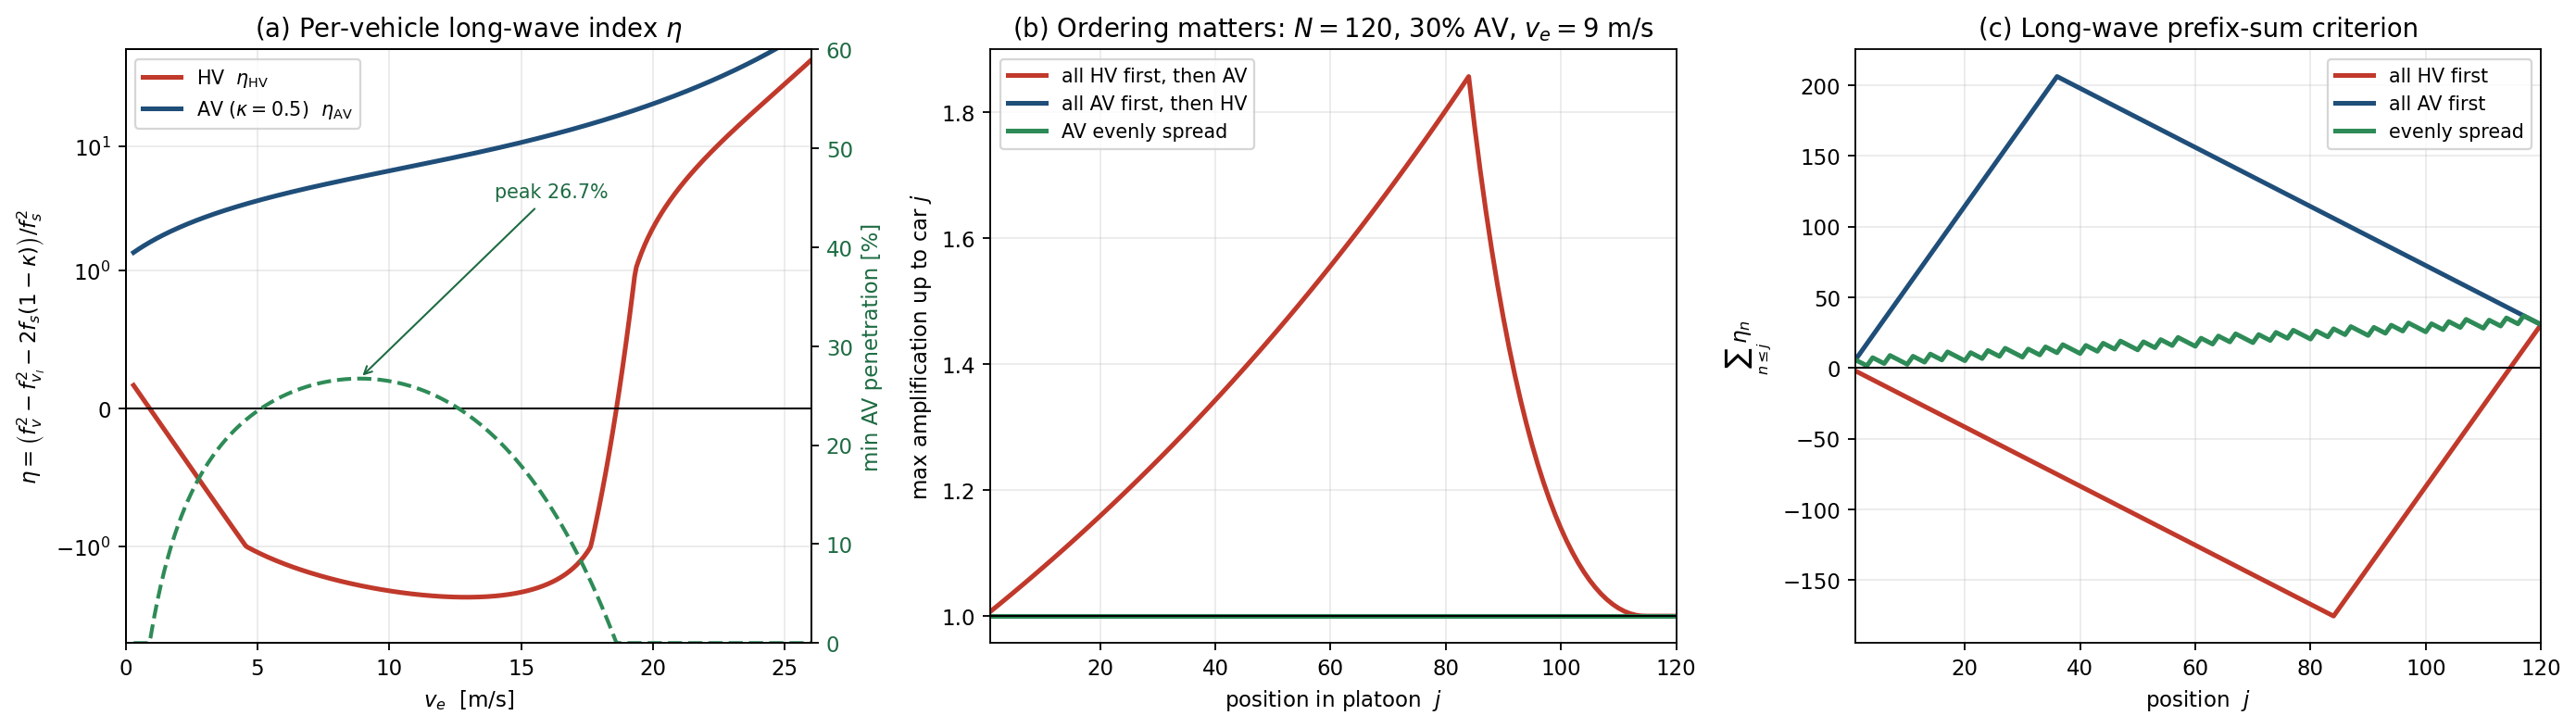
\includegraphics[width=\textwidth]{fig8.png}
\caption{异质车队的总预算与排序效应。}
\label{fig:heter-order-budget}
\figurenote{异质车队中“总配方”和“车辆排序”分别控制什么。左图沿平衡速度计算 HDV 与 AV 的长波指数，并由加权总和求最低 AV 渗透率；曲线在约 $v_e=9$ m/s 达到最不利峰值 26.7\%，说明渗透率阈值必须覆盖速度工作域，而不能只在一个方便工况读取。中图固定 $N=120$、30\% AV，比较三种排序的逐车累计放大：三条曲线到末端都回到 1，验证固定标量 $G_n$ 时整圈乘积与排列无关；但将 84 辆 HDV 放在传播路径前段时，中途峰值达到 1.857。右图的长波前缀和解释了这一峰值来源：不稳定 HDV 的负贡献先累积，直到后续 AV 的正贡献才把总和拉回非负。该图证明环道只要求最终总预算非负，而开放车队若关心任何中间车辆都不放大，就必须检查所有前缀；“末端稳定”不能替代“途中安全”。}
\end{figure}

图中“队首”并非环道天然存在的头车，而是把环道在扰动注入点切开后，沿扰动传播方向的第一个位置。该工况有 84 辆 HDV 与 36 辆 AV，且
\[
\eta_{\rm HDV}=-2.088,
\qquad
\eta_{\rm AV}=5.724,
\qquad
S_{120}=84(-2.088)+36(5.724)=30.672>0.
\]
因此三种排列的整圈总预算相同。若 HV 全在前，则
\[
S_{84}=84(-2.088)=-175.392,
\qquad
S_{84+r}=-175.392+5.724r.
\]
直到第 31 辆 AV 出现，即 $j=115$，前缀和才由负转正；所以该排列在 $j=1,\ldots,114$ 均违反式~\eqref{eq:heter-prefix}。若 AV 全在前，则先积累 $S_{36}=206.064$ 的正预算，后续 84 辆 HDV 虽持续消耗它，直到末端仍保持 $S_j\ge0$。均匀排列通过缩短连续 HV 段达到同一目的。

“末端为 $1.0000$”也不能解释成所有频率均原样通过。图中纵轴是 $\max_{\omega\ge0}|H_j(i\omega)|$；因为 $G_n(0)=1$，任何稳定前缀在 $\omega=0$ 都有增益 1，而非零频率的增益小于 1，所以最大值显示为 1.0000。红色排列在有限非零频率处超过 1，才出现 1.857 的峰值。

\begin{tcolorbox}[keybox,title=\textbf{核心结论}]
\begin{equation}
\prod_{n=1}^{N}\left|G_n\right| \ \text{与排序无关（乘积可交换）},
\qquad
\max_j\left|\prod_{n\le j}G_n\right| \ \text{强烈依赖排序}
\end{equation}
\begin{itemize}[leftmargin=1.2em,itemsep=3pt]
\item \textbf{环道渐近稳定：检查 $j=N$。} 固定每辆车的 $G_n$ 后，完整乘积可交换，所以特征方程与整圈总增益只看配方，不看排列。
\item \textbf{开放车队／内部无放大：检查所有 $j$。} 本例三种排列末端都是 $1.0000$，但 HV 集中在传播路径前段时中途放大到 $1.857$，故它不满足式~\eqref{eq:heter-prefix}，即使环道最终仍衰减。
\item \textbf{$26.7\%$ 只回答总量，不回答排序。} 它保证 $S_N\ge0$；在此前提下仍需把 AV 放在扰动路径前段或尽量均匀分散，避免 $S_j$ 中途跌破零。
\end{itemize}
\end{tcolorbox}

\section{AV 的加速度反馈：前馈能力取决于前车类型}
\sectionstudy{model}{AV 的加速度反馈：前馈能力取决于前车类型}{talebpour2016,feng2019,stern2018}
\label{sub:mixed}

上面把 $f_a^{(n)}$ 当成该车自身的属性。但在混合车流中这个假设过于乐观：\textbf{前馈需要前车提供加速度信息}，而信息质量取决于\textbf{前车是什么车}。

\begin{table}[htbp]
\centering
\small
\caption{AV/HDV 相邻组合与实际前馈增益。}
\label{tab:pair-dependent-gain}
\begin{tabular}{p{4.4cm}p{4.4cm}p{4.6cm}}
\toprule
第 $n$ 辆是 & 第 $n-1$ 辆是 & 有效增益 $f_a^{(n)}$ \\
\midrule
HV & 任意 & $0$ \\
AV & AV（可 V2V 广播） & $\kappa$（完整，低噪声低延迟） \\
AV & HV（只能雷达估计） & $\kappa_0<\kappa$（微分噪声大，须保守） \\
\bottomrule
\end{tabular}
\end{table}

表~\ref{tab:pair-dependent-gain} 给出了本章采用的相邻对规则：HDV 不使用前馈，AV 跟随 AV 时获得完整 V2V 增益 $\kappa$，AV 跟随 HDV 时只能使用雷达估计增益 $\kappa_0$。因此，同样数量的 AV 只要相邻结构不同，就会产生不同的有效控制总量。

\begin{tcolorbox}[notebox,title=\textbf{这带来一个结构性的新效应}]
$\eta_n$ 现在依赖\textbf{相邻两辆车的组合}，而不只是本车类型。于是
\[
\sum_{n}\eta_n = N_H\,\eta_{\rm HV} + \left(N_A-q\right)\eta_{\rm AV}^{(\kappa_0)} + q\,\eta_{\rm AV}^{(\kappa)}
\]
其中 $q$ 是车队中\textbf{AV--AV 相邻对的数目}。\textbf{连总和都变得依赖排序了}——这与 \S\ref{sub:hetorder} 的"总放大与排序无关"形成对照，因为那里假设 $\eta_n$ 是固定的。
\end{tcolorbox}

\subsection{渗透率：分散布置的代价}

回顾 $\eta_{\rm AV}^{(\kappa)} = \eta_{\rm HV} + 2\kappa/f_s$。对第~\ref{sec:num}~章的 IDM 参数，取 $\kappa=0.5$（V2V）与 $\kappa_0=0.15$（雷达估计）：

\begin{table}[htbp]
\centering
\caption{孤立 AV 与连续编组所需渗透率的速度依赖。}
\label{tab:dispersed-versus-grouped-pmin}
\begin{tabular}{rccccc}
\toprule
$v_e$ [m/s] & $f_s$ & $\eta_{\rm HV}$ & $\eta_{\rm AV}^{(\kappa_0)}$ & $\eta_{\rm AV}^{(\kappa)}$ & $p_{\min}$（分散／编组） \\
\midrule
3  & 0.308 & $-0.574$ & $+0.401$ & $+2.676$ & 58.9\% \ / \ 17.7\% \\
6  & 0.182 & $-1.378$ & $+0.274$ & $+4.130$ & 83.4\% \ / \ 25.0\% \\
9  & 0.128 & $-2.088$ & $+0.255$ & $+5.724$ & \textbf{89.1\%} \ / \ \textbf{26.7\%} \\
12 & 0.098 & $-2.532$ & $+0.546$ & $+7.727$ & 82.3\% \ / \ 24.7\% \\
16 & 0.071 & $-2.010$ & $+2.224$ & $+12.10$ & 47.5\% \ / \ 14.2\% \\
\bottomrule
\end{tabular}
\end{table}

表~\ref{tab:dispersed-versus-grouped-pmin} 给出了两种极端布置的长波预算。逐辆分散时，几乎所有 AV 都只能使用 $\kappa_0$，在 $v_e=9$ m/s 附近所需比例达到 89.1\%；连续编组让大部分 AV 获得 $\kappa$，对应门槛降至 26.7\%。该差异说明渗透率必须与通信邻接结构共同报告。

\begin{tcolorbox}[keybox,title=\textbf{核心数字}]
全速域长波总预算所需的最小渗透率：\textbf{逐辆分散 $89.1\%$，连续编组 $26.7\%$。} 给定比例和编组后仍须检查前缀峰值。

差了三倍多。原因很直白：孤立的 AV 前面永远是 HV，永远只能拿到降级的 $\kappa_0$；而编组内部的 AV 彼此可以 V2V。
\end{tcolorbox}

\subsection{AV 渗透率--速度二维稳定域}
\label{sub:av-plane}

只报告一个“临界 AV 渗透率”仍然不够，因为临界比例随平衡速度显著变化。更完整的做法是把 AV 渗透率 $p_{\rm AV}$ 与平衡速度 $v_e$ 同时作为坐标，在每一个工作点重新计算 IDM 偏导、AV--AV／AV--HDV 相邻对数以及全频率传播增益，从而得到二维稳定域
\begin{equation}
\mathcal S_{\rm AV}
=\left\{(p_{\rm AV},v_e):M_{\rm L}(p_{\rm AV},v_e)\ge0,
\ M_{\rm T}(p_{\rm AV},v_e)\ge0\right\}.
\label{eq:av-stability-set}
\end{equation}

对给定排列，第 $n$ 辆车的实际前馈增益不是一个平均常数，而是
\begin{equation}
a_n\in\{0,\kappa_0,\kappa\},
\qquad
a_n=
\begin{cases}
0, & n\text{ 为 HDV},\\
\kappa_0, & n\text{ 为 AV、前车为 HDV},\\
\kappa, & n\text{ 为 AV、前车为 AV}.
\end{cases}
\label{eq:av-pair-gain}
\end{equation}
因此二维图采用两个互补裕度。第一个是长波裕度
\begin{equation}
M_{\rm L}
=\frac1N\sum_{n=1}^{N}
\left[f_v^2-f_{v_l}^2-2f_s(1-a_n)\right],
\label{eq:av-long-margin}
\end{equation}
它决定 $\omega\to0$ 时扰动是否增长。第二个是实际环周传递裕度
\begin{align}
G_n(i\omega)
&=\frac{f_s-a_n\omega^2+i\omega f_{v_l}}
{f_s-\omega^2-i\omega f_v},\\
M_{\rm T}
&=\min_{\omega>0}
\left[-\frac1N\sum_{n=1}^{N}\ln|G_n(i\omega)|\right].
\label{eq:av-transfer-margin}
\end{align}
$M_{\rm T}>0$ 表示扰动绕环一周后衰减，$M_{\rm T}<0$ 表示至少有一个频率绕环一周后被放大。式~\eqref{eq:av-stability-set} 同时要求二者非负，是为了既不漏掉极低频长波，也不把“长波稳定但有限频率放大”的工况误涂成稳定。

\begin{figure}[htbp]
\centering
\begin{tabular}{cc}
\textbf{(a) 无前馈：$\kappa=0$} &
\textbf{(b) 混合交通：$\kappa=0.45,\ \kappa_0=0.15$}
\end{tabular}
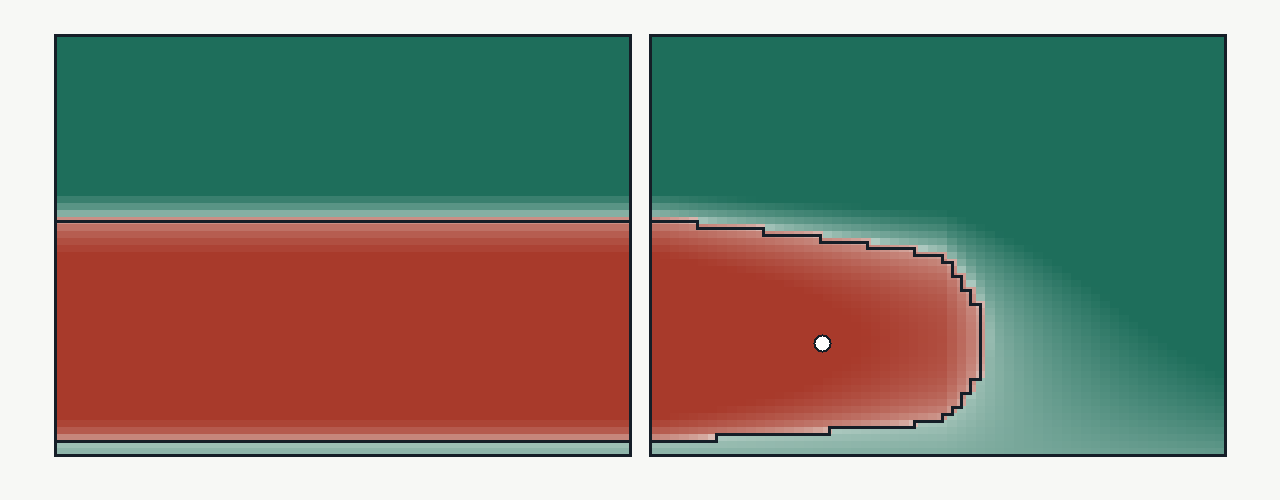
\includegraphics[width=\textwidth]{av_penetration_speed_plane.png}
\vspace{-0.4em}

\small
横轴：$p_{\rm AV}=0\to100\%$；纵轴：$v_e=0\to33.3$ m/s；
\textcolor{teal}{\rule{1.1em}{0.75em}} 稳定，
\textcolor{brick}{\rule{1.1em}{0.75em}} 失稳，黑线为边界，白点为当前工作点。
\caption{AV 渗透率--速度二维稳定域。}
\label{fig:av-stability-plane}
\figurenote{AV 渗透率--平衡速度二维稳定平面及其因果对照。两图均取 $N=60$ 并按同一规则均匀排列 AV，颜色表示由长波预算和全频传递裕度共同确定的稳定／失稳区域。左图故意令 $\kappa=0$：即使横轴上的 AV 比例改变，车辆动力学并未改变，稳定边界仍退化为原始 IDM 的水平分界；这证明“AV 标签”本身不会产生稳定收益。右图启用 $\kappa$ 与 $\kappa_0$ 后，增加 AV 比例使稳定区向原本危险的中低速范围扩展，但同一渗透率在不同速度下仍可能一稳一失，说明阈值必须是二维工作域概念。边界上的细小台阶对应 $N=60$ 时 AV 数量和 AV--AV 相邻对数的整数跳变，而非求解噪声。该图证明稳定域扩大来自可用前馈链路及其邻接结构，并为给定速度范围读取最低渗透率提供了直接工具。}
\end{figure}

\begin{tcolorbox}[experimentbox,title=\textbf{二维平面的具体读数}]
取图~\ref{fig:av-stability-plane}(b) 的参数。在 $p_{\rm AV}=30\%$、$v_e=8.87$ m/s 时，实际平均前馈仅为 $0.0450$，得到
$M_{\rm L}=-0.02300$、$M_{\rm T}=-0.00233$，故该点仍失稳；白点落在红区。把工作点移到 $p_{\rm AV}=73\%$、$v_e=14.42$ m/s 时，平均前馈增至 $0.2500$，得到
$M_{\rm L}=+0.02432$、$M_{\rm T}=+0.00865$，故转为稳定。这个对照说明“AV 比例相同”并不能脱离速度讨论，“平均增益相同”也不能代替真实相邻对序列的环周乘积。
\end{tcolorbox}

\begin{tcolorbox}[notebox,title=\textbf{如何使用这张图}]
\begin{enumerate}[leftmargin=1.5em,itemsep=3pt]
\item 先给出道路的速度工作域，例如 $v_e=5$--$20$ m/s；不要只在一个名义速度上求 $p_{\min}$。
\item 在该速度带内取稳定边界最靠右的位置，得到覆盖全工作域的最小渗透率；若只关心某一速度，则读取该水平截线与黑色边界的交点。
\item 改变 $\kappa$、$\kappa_0$、排列方式或编组数后必须重画。尤其在相邻对规则下，$p_{\rm AV}$ 只决定有多少辆 AV，排列决定这些 AV 实际拿到 $\kappa$ 还是 $\kappa_0$。
\item 边界附近必须留出正裕度，并用 1800 s 时域仿真复核；二维图是小扰动稳定域，不是碰撞安全域，也不保证任意大扰动都能恢复。
\end{enumerate}
\end{tcolorbox}

\textbf{这与 \S\ref{sub:hetorder} 的建议直接冲突：} 那里说"把稳定车辆均匀分散"，这里说"必须成组"。真实的设计问题是在两者之间取平衡。

\section{最优编组尺寸：先说明“最优”针对什么目标}
\sectionstudy{theory}{最优编组尺寸：先说明“最优”针对什么目标}{talebpour2016,feng2019,stern2018}
\label{sec:optimal-grouping}

“AV 应分成几组”没有脱离目标函数的唯一答案。组数少时，组内 AV--AV 相邻对多，完整 V2V 增益 $\kappa$ 被充分利用，因而\textbf{整圈总稳定预算更大}；组数多时，AV 在道路空间上更分散，连续 HDV 段更短，因而\textbf{扰动在遇到稳定车辆以前的途中放大更小}。这两个方向彼此竞争，必须首先区分以下两个问题：
\[
\begin{aligned}
\text{问题 A：}&\max_{1\le g\le N_A} S_N(g),\\
\text{问题 B：}&\min_{1\le g\le N_A}H_{\max}(g)
\quad\text{s.t.}\quad S_N(g)\ge S_{\rm res}.
\end{aligned}
\]
问题 A 只追求总稳定裕度，其答案必然是把全部 AV 合成一组，即 $g=1$。问题 B 则先规定必须保留的稳定储备 $S_{\rm res}\ge0$，再尽量缩短最长连续 HDV 段；只有在问题 B 下，答案才是“取满足稳定预算的最大可行组数”。本节所称“最优编组”专指上述问题 B 的\textbf{字典序目标：先保证总预算，再改善空间覆盖}，而不是声称多分组可以让总稳定裕度更大。

\subsection{从相邻对计数推导组数上限}

设 $N_A$ 辆 AV 被分成 $g=n_{\rm grp}$ 个非空组。每个组若含 $h_r$ 辆 AV，就贡献 $h_r-1$ 个 AV--AV 相邻对；因此无论各组长度是否相等，
\begin{equation}
q=\sum_{r=1}^{g}(h_r-1)=N_A-g.
\label{eq:group-pair-count}
\end{equation}
其余 $g$ 辆位于组边界的 AV 跟随 HDV，只能使用降级增益 $\kappa_0$。整圈长波预算因而是
\begin{align}
S_N(g)
&=N_H\eta_{\rm HV}+(N_A-g)\eta_{\rm AV}^{(\kappa)}
  +g\eta_{\rm AV}^{(\kappa_0)} \\
&=C-g\,\Delta\eta,
\qquad
C:=N_H\eta_{\rm HV}+N_A\eta_{\rm AV}^{(\kappa)},
\quad
\Delta\eta:=\eta_{\rm AV}^{(\kappa)}-\eta_{\rm AV}^{(\kappa_0)}>0.
\label{eq:group-budget-linear}
\end{align}
式~\eqref{eq:group-budget-linear} 表明：\textbf{每多切出一组，恰好损失一份 $\Delta\eta$ 的总稳定预算}。原因是新组会多产生一辆“位于组首、前车为 HDV”的 AV：该车原本处在 AV--AV 相邻对中，可以取得 $\kappa$；切组后只能取得 $\kappa_0$，所以它对总和的贡献由 $\eta_{\rm AV}^{(\kappa)}$ 降为 $\eta_{\rm AV}^{(\kappa_0)}$。

先取没有额外储备的理论边界 $S_{\rm res}=0$。要求 $S_N(g)\ge0$，由 $C-g\Delta\eta\ge0$ 依次得到
\[
g\Delta\eta\le C,
\qquad
g\le\frac{C}{\Delta\eta}.
\]
把 $C=N_H\eta_{\rm HV}+N_A\eta_{\rm AV}^{(\kappa)}$ 和 $\Delta\eta=\eta_{\rm AV}^{(\kappa)}-\eta_{\rm AV}^{(\kappa_0)}$ 代回，就得到
\begin{tcolorbox}[keybox,title=\textbf{组数上限与整数可行解}]
\begin{align}
g&\le g_{\max}
=\frac{N_A\eta_{\rm AV}^{(\kappa)}+N_H\eta_{\rm HV}}
{\eta_{\rm AV}^{(\kappa)}-\eta_{\rm AV}^{(\kappa_0)}}
=\frac{f_s\left(N_A\eta_{\rm AV}^{(\kappa)}+N_H\eta_{\rm HV}\right)}
{2(\kappa-\kappa_0)}, \\
g^*&=\min\!\left\{N_A,\left\lfloor g_{\max}\right\rfloor\right\},
\qquad S_N(g^*)\ge0.
\label{eq:optimal-group-count}
\end{align}
\end{tcolorbox}
式~\eqref{eq:optimal-group-count} 的第二个等号使用了
\[
\eta_{\rm AV}^{(\kappa)}-\eta_{\rm AV}^{(\kappa_0)}
=\frac{2(\kappa-\kappa_0)}{f_s}.
\]
因此 $g_{\max}$ 可以直接读成“全部 AV 连成一组时可用的总稳定预算”除以“每增加一组损失的稳定预算”。这里还隐含两项可行性检查：编组至少需要 $g\ge1$；若 $g_{\max}<1$，说明即使把全部 AV 合成一个组，总预算仍不足，不存在满足当前约束的布置。其次，$g$ 必须是整数且不超过 $N_A$，所以要取下整并与 $N_A$ 比较。此时应提高 AV 渗透率、$\kappa$ 或 $\kappa_0$，而不能把 $g^*=0$ 解释成一种道路布置。

\subsection{为什么一个大组总裕度最好，却不一定最抗途中放大}

先看问题 A。由式~\eqref{eq:group-budget-linear}，
\[
S_N(g+1)-S_N(g)=-\Delta\eta<0,
\]
所以 $S_N(g)$ 随 $g$ 严格下降。如果唯一目标是最大化整圈总稳定预算，那么结论毫无歧义：$g=1$ 最好。全部 AV 连成一个组保留了最多的 AV--AV 相邻对，也给出了最大的绕环衰减储备。

问题在于，总预算只描述扰动完成整条传播路径后的净结果，并不限制它在途中先放大多少。一个大 AV 组意味着其余 HDV 往往形成很长的连续区段；若扰动从该区段进入，就可能在遇到 AV 以前逐车放大。即使末端最终衰减，中途峰值仍会影响速度波动、制动强度、间距和能耗。因此，问题 B 还要控制最长连续 HDV 段。

固定组数 $g$ 后，把 $N_H$ 辆 HDV 分配到 $g$ 个组间空档。由抽屉原理，最长连续 HDV 段 $H_{\max}$ 必满足
\begin{equation}
H_{\max}\ge\left\lceil\frac{N_H}{g}\right\rceil,
\label{eq:group-pigeonhole}
\end{equation}
而近似均匀地放置各 AV 组可以达到该下界。由于 $\lceil N_H/g\rceil$ 随 $g$ 增大而不增，在所有满足 $S_N(g)\ge S_{\rm res}$ 的方案中，取最大的整数 $g$ 能把最坏连续 HDV 段压到最短，也就使任意位置产生的扰动更早遇到一段稳定 AV。另一方面，式~\eqref{eq:group-budget-linear} 又说明 $g$ 不能无限增加。因此，对问题 B 而言，一个指标随 $g$ 改善、另一个约束随 $g$ 收紧，解必落在稳定预算边界，而不是内部某个任意组数。

还要注意扰动源是否已知。如果主要扰动总从一个固定入口进入，把单个大 AV 组放在该输入端附近可能同时获得高总裕度和低前缀峰值，此时 $g=1$ 完全可能更合适；若扰动可能从多个位置出现，或研究环道中的随机扰动，则均匀分散的多组方案更具空间鲁棒性。因此“多组更优”依赖于未知／多源扰动假设，而不是一个普遍定理。

这个“最优”有明确边界：它只针对“总长波预算达到指定储备 $+$ 最短最坏 HDV 段”的目标。若需给模型误差、通信丢包或有限频率模态留出正裕度 $S_{\rm res}>0$，应改用
\begin{equation}
g_{\rm robust}^*
=\left\lfloor\frac{C-S_{\rm res}}{\Delta\eta}\right\rfloor,
\label{eq:robust-group-count}
\end{equation}
所以工程最优组数可能比理论最大值少一组。若还显式计入通信成本、编组维护成本、换道扰动或已知扰动源位置，则需建立新的多目标函数，不能把式~\eqref{eq:optimal-group-count} 当成无条件的全局最优。概括来说：\textbf{$g=1$ 最大化总稳定裕度；$g=g_{\max}$ 在维持规定裕度的前提下最大化空间覆盖。}

\subsection{数值算例：为什么理论为 5 组、试验选 4 组}

取 $N=120$、$N_A=36$、$N_H=84$、$v_e=9$ m/s，式~\eqref{eq:optimal-group-count} 给出 $g_{\max}=5.6$，因此纯解析约束下 $g^*=5$。36 辆 AV 可分为 $8+7+7+7+7$，84 辆 HDV 的五个间隔可分为 $17+17+17+17+16$，故最长 HDV 段从单组方案的 84 辆降至 17 辆。由于 5 组非常接近稳定边界，后续时域试验采用 4 组作为留有裕度的稳健方案；此时最长 HDV 段约为 21 辆。

\begin{table}[htbp]
\centering
\caption{不同 AV 编组方案的总预算与传播增益。}
\label{tab:grouping-alternatives}
\begin{tabular}{lcccc}
\toprule
布置 & $q$ & $\sum_n\eta_n$ & 中途峰值 & 末端 \\
\midrule
1 组置于\textbf{队首} & 35 & $+25.2$ & $1.000$ & $1.0000$ \\
1 组置于\textbf{队尾} & 35 & $+25.2$ & \textbf{1.857} & $1.0000$ \\
4 组均布 & 32 & $+8.8$ & $1.000$ & $1.0000$ \\
8 组均布 & 24 & $-44.4$ & $1.032$ & $1.0322$ \\
逐辆分散 & 0 & $-166.2$ & $1.513$ & $1.5130$ \\
\bottomrule
\end{tabular}
\end{table}

表~\ref{tab:grouping-alternatives} 给出了组数增加时“空间覆盖改善、V2V 总预算下降”的竞争关系。单组置于队首和队尾具有相同 $q$ 与末端增益，但队尾方案的中途峰值达到 1.857，说明组数之外还要决定相对于扰动源的位置；4 组均布仍保有正预算且无中途放大，8 组则已经越过解析上限而失稳。

\begin{figure}[htbp]
\centering
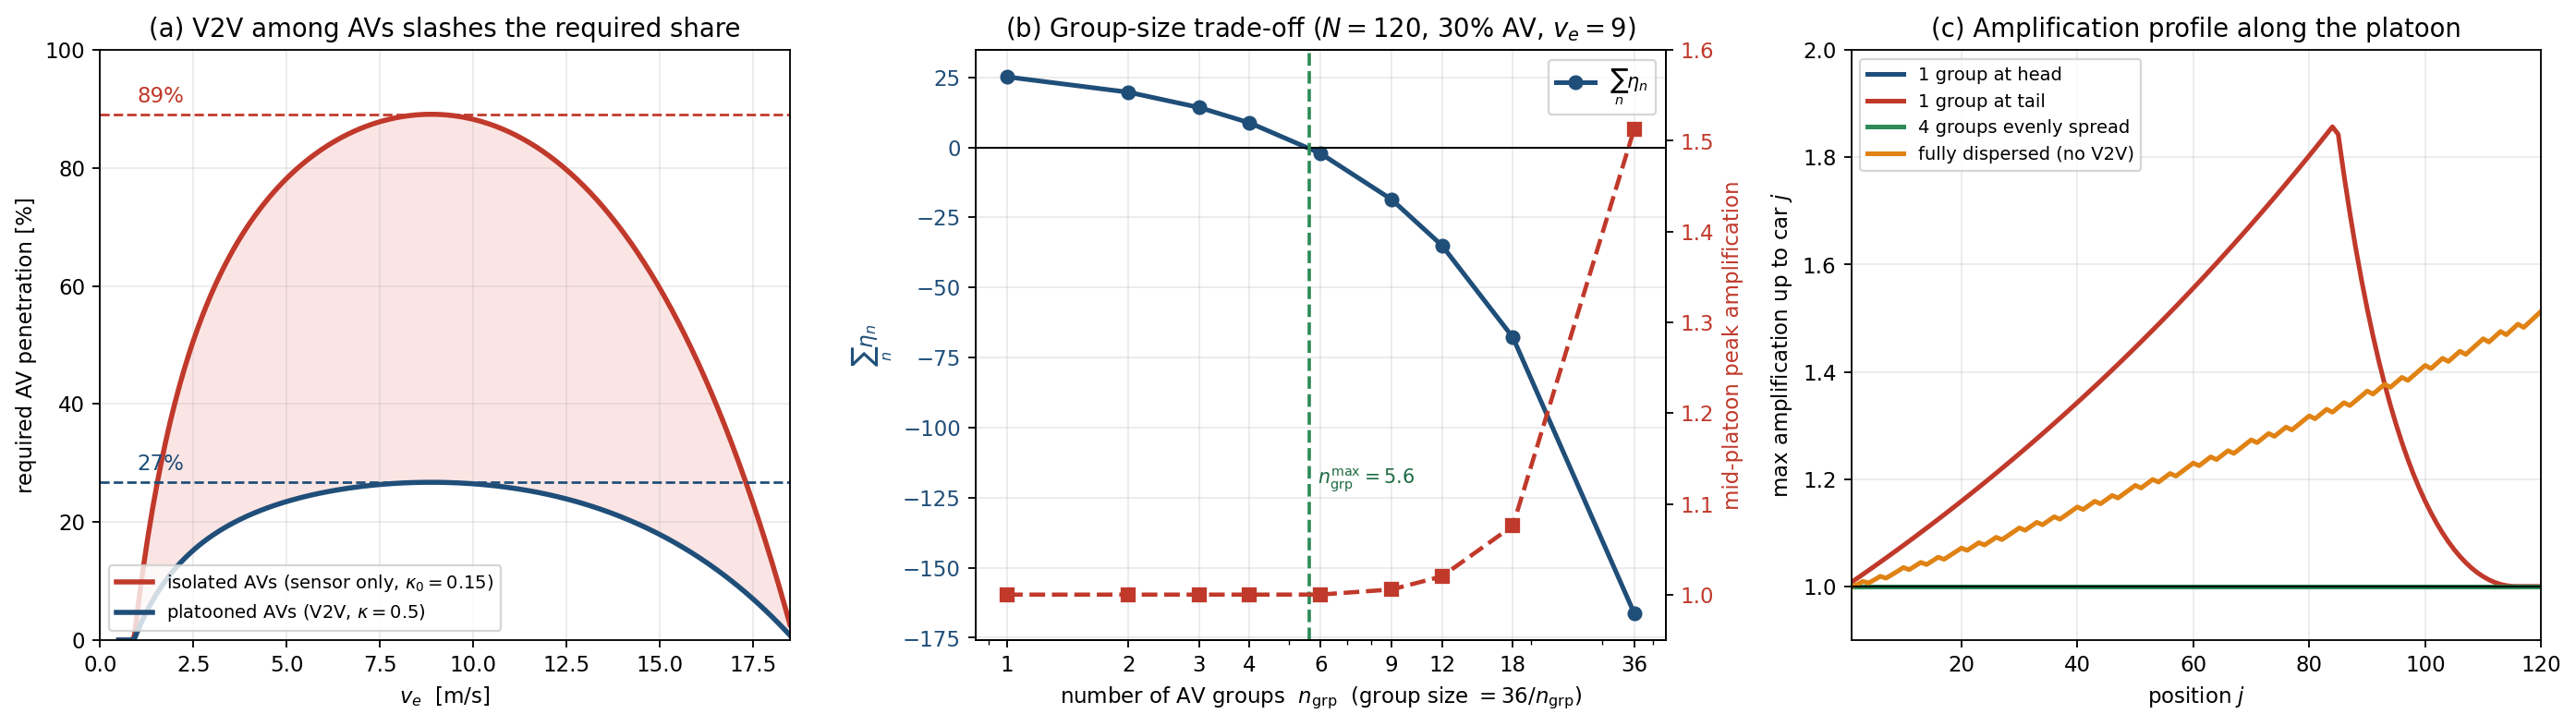
\includegraphics[width=\textwidth]{fig9.png}
\caption{AV 编组数量、渗透率与途中放大的权衡。}
\label{fig:av-grouping}
\figurenote{AV 编组问题中总裕度、空间覆盖与扰动源位置的三重权衡。左图比较孤立 AV 只能用雷达估计增益 $\kappa_0$ 与成组 AV 可通过 V2V 使用完整增益 $\kappa$ 的两条最低渗透率曲线；最不利速度附近的需求由约 89\% 降至约 27\%，证明决定收益的不是 AV 数量本身，而是形成了多少 AV--AV 通信相邻对。中图固定 36 辆 AV，横轴增加组数：蓝色总预算 $S_N$ 近似线性下降并在 $g_{\max}\approx5.6$ 附近越过零线，而最长 HDV 段随组数增加而缩短；这直接展示上述问题 A“最大化总裕度”与问题 B“在裕度约束下改善空间覆盖”的冲突。右图比较同一个 AV 大组放在扰动输入端和传播末端：两者末端总增益相同，但末端布置在遇到 AV 前先放大到 1.857，说明总和相同并不保证前缀暴露相同。该图证明：若目标仅是最大总裕度，$g=1$ 最优；若在保留规定裕度后还要防御未知位置扰动，则应增加到最大可行组数并近似均匀布置。}
\end{figure}

\begin{tcolorbox}[keybox,title=\textbf{最优编组的两步设计准则}]
\begin{enumerate}[leftmargin=1.6em,itemsep=3pt]
\item 由式~\eqref{eq:optimal-group-count} 或带裕度的式~\eqref{eq:robust-group-count} 计算组数上限，先保证总稳定预算。
\item 在可行组数内取最大值，并把各组和 HDV 间隔尽量均匀，以最小化最长连续 HDV 段及前缀峰值。
\item 若只能布置一个大组，应把它放在主要扰动输入端附近；本例置于队尾会把中途峰值提高 85.7\%。
\item 提高 $\kappa_0$ 会减小 $\Delta\eta$，允许更多、更分散的编组；这说明改善 AV 对 HDV 加速度的估计质量具有直接的拓扑价值。
\end{enumerate}
\end{tcolorbox}

\section{多前车 AV：从标量传递函数到传递矩阵}
\sectionstudy{theory}{多前车 AV：从标量传递函数到传递矩阵}{swaroop1996,ploeg2014,feng2019}
\label{sec:heter-multileader}

最近邻前馈时，第 $n$ 辆车只依赖第 $n-1$ 辆车，因此一个标量 $G_n=Y_n/Y_{n-1}$ 就能逐车相乘。若 AV 同时接收前方 $m$ 辆车的加速度广播，$Y_n$ 同时依赖 $Y_{n-1},\ldots,Y_{n-m}$；此时不存在唯一的标量输入，必须把连续 $m$ 个车辆扰动组成状态向量。

\subsection{从线性化跟驰方程到矩阵递推}

只考虑多前车\textbf{加速度}前馈，并保留最近前车提供的间距与相对速度刺激。异质车队的线性化方程为
\begin{equation}
\ddot y_n
=f_s^{(n)}(y_{n-1}-y_n)+f_v^{(n)}\dot y_n
+f_{v_l}^{(n)}\dot y_{n-1}
+\sum_{r=1}^{m}a_{n,r}\ddot y_{n-r},
\label{eq:heter-multi-time}
\end{equation}
其中 $a_{n,r}=0$ 表示第 $n$ 辆车没有接收到第 $r$ 辆前车的信息。取零初值 Laplace 变换并整理含 $Y_n$ 的项，得到
\begin{equation}
D_n(\lambda)Y_n
=\sum_{r=1}^{m}N_{n,r}(\lambda)Y_{n-r},
\qquad
D_n=\lambda^2-f_v^{(n)}\lambda+f_s^{(n)},
\label{eq:heter-multi-laplace}
\end{equation}
其中
\begin{equation}
N_{n,1}=f_s^{(n)}+f_{v_l}^{(n)}\lambda+a_{n,1}\lambda^2,
\qquad
N_{n,r}=a_{n,r}\lambda^2\quad(r\ge2).
\label{eq:heter-multi-numerators}
\end{equation}
第一辆前车同时提供普通跟驰刺激和加速度广播，所以 $N_{n,1}$ 含三项；更远前车在本模型中只提供广播加速度，因此其分子只有 $a_{n,r}\lambda^2$。

定义
\begin{equation}
Z_n:=\begin{pmatrix}Y_n&Y_{n-1}&\cdots&Y_{n-m+1}\end{pmatrix}^{\!\mathsf T},
\end{equation}
则式~\eqref{eq:heter-multi-laplace} 等价于伴随矩阵递推
\begin{equation}
Z_n=M_n(\lambda)Z_{n-1},
\qquad
M_n(\lambda)=
\begin{pmatrix}
N_{n,1}/D_n&N_{n,2}/D_n&\cdots&N_{n,m}/D_n\\
1&0&\cdots&0\\
0&1&\ddots&\vdots\\
\vdots&\ddots&\ddots&0
\end{pmatrix}.
\label{eq:heter-multi-matrix}
\end{equation}
当 $m=1$ 时，$M_n$ 退化为 $1\times1$ 的 $G_n$；当 $m=2$ 时，第一行就是原稿中的两个分式，第二行只负责把 $Y_{n-1}$ 向后移一格。所谓“传递函数退化为传递矩阵”，本质上是系统的空间记忆阶数由 1 增加到 $m$。

\subsection{开放车队与环道的稳定条件}

从扰动源传播到第 $j$ 辆车的矩阵为有序乘积
\begin{equation}
\mathcal M_j(\lambda)=M_j(\lambda)M_{j-1}(\lambda)\cdots M_1(\lambda),
\qquad Z_j=\mathcal M_jZ_0.
\label{eq:heter-multi-prefix}
\end{equation}
开放车队若要求任意组合输入都不被放大，可用诱导二范数的充分条件
\begin{equation}
\sup_{\omega>0}\left\|\mathcal M_j(i\omega)\right\|_2\le1
\qquad \forall j.
\label{eq:heter-multi-open-condition}
\end{equation}
该条件比指定某一输入方向更保守，但能覆盖 $m$ 个历史车辆扰动的任意线性组合。

对环道，传播一圈后状态向量必须恢复自身，因此
\begin{tcolorbox}[keybox,title=\textbf{多前车异质环道的闭合方程}]
\begin{equation}
\det\!\left[\mathcal M_N(\lambda)-I_m\right]=0,
\qquad
\mathcal M_N=M_NM_{N-1}\cdots M_1.
\label{eq:heter-multi-ring}
\end{equation}
\end{tcolorbox}
应求式~\eqref{eq:heter-multi-ring} 的全部根，并排除整体平移对应的 $\lambda=0$。由于 $M_n$ 含有 $D_n$ 的分母，实际计算宜直接组装原始 $2N$ 维线性状态矩阵求本征值，或在清分母后核对是否引入伪根；只扫描 $\|\mathcal M_N(i\omega)\|_2$ 是小增益筛选，不是完整的必要条件。

\subsection{均匀车队极限：重新得到多前车 Fourier 判据}

若所有车辆参数与权重都相同，令
\[
y_n(t)=\widehat y\,e^{\lambda t+ikn},
\qquad y_{n-r}=e^{-irk}y_n.
\]
将其直接代入式~\eqref{eq:heter-multi-time}，得到
\begin{equation}
\underbrace{\left(1-\sum_{r=1}^{m}a_r e^{-irk}\right)}_{P_m(k)}\lambda^2
-\underbrace{\left(f_v+f_{v_l}e^{-ik}\right)}_{Q(k)}\lambda
-\underbrace{f_s\left(e^{-ik}-1\right)}_{R(k)}=0.
\label{eq:heter-multi-uniform-dispersion}
\end{equation}
这正是第~\ref{sec:multi}~章的多前车色散关系。也就是说，传递矩阵并没有创造另一套理论：均匀时矩阵的空间本征向量就是 Fourier 模态，异质时因为 $M_n$ 随车辆变化，才不能用一个共同波数把它们同时对角化。

记权重的零阶矩与一阶矩为
\begin{equation}
m_0=\sum_{r=1}^{m}a_r,
\qquad
m_1=\sum_{r=1}^{m}r a_r.
\end{equation}
长波展开给出必要门槛
\begin{equation}
\frac{f_v^2-f_{v_l}^2}{2}\ge(1-m_0)f_s,
\label{eq:heter-multi-longwave}
\end{equation}
所以总增益 $m_0$ 决定长波能否稳定；在固定 $m_0$ 下，把权重移向更远前车会增大 $m_1$，通常抬高有限波长裕度。但式~\eqref{eq:heter-multi-longwave} 只是必要条件，仍需对式~\eqref{eq:heter-multi-uniform-dispersion} 的全部离散 $k$ 求根。

\subsection{为什么多前车后排序连末端都可能改变}

最近邻标量情形中 $\prod_nG_n$ 可交换，固定车辆属性后末端总增益与排序无关。多前车情形中一般有
\begin{equation}
M_AM_H\ne M_HM_A,
\end{equation}
因为某辆 AV 的两个输入槽位会跨越不同的车型边界。因此交换两辆车会改变整圈矩阵 $\mathcal M_N$ 的特征值和奇异值，连环道闭合根与末端总放大都可能变化。相邻对计数 $q$ 和标量预算 $S_N$ 只能作为最近邻近似，不能替代矩阵判定。

\begin{tcolorbox}[experimentbox,title=\textbf{多前车稳定性的推荐计算流程}]
先给定车辆顺序和每辆 AV 可接收的前车集合；再按式~\eqref{eq:heter-multi-matrix} 构造各 $M_n(i\omega)$，扫描所有前缀的最大奇异值以评价途中放大；随后直接组装 $2N$ 维状态矩阵求最右特征值，验证环道渐近稳定；最后以相同排序进行 1800 s 非线性 IDM 仿真。只有“矩阵频域、特征值和时域”三者符号一致，才能把多前车方案判为可靠稳定。
\end{tcolorbox}

\section{适用边界}
\sectionstudy{synthesis}{适用边界}{talebpour2016,feng2019,stern2018}

\begin{itemize}[leftmargin=1.4em,itemsep=3pt]
\item \textbf{异质 $+$ 双向耦合}：级联结构与循环对称性同时消失，标量传递函数和空间 Fourier 两类简化均不再适用，需要直接求 $2N$ 维系统的本征值。
\item \textbf{异质 $+$ 延迟}：逐车传递函数仍可写（分子分母各带 $e^{-\lambda\tau_n}$），逐车判据 $\Psi_n(\omega)\ge0$ 与前缀积条件都照常成立。
\item \textbf{车序随机}：若无法控制排列，只能退回条件 (ii) 的逐车严格线稳定，或对随机排列做概率界。
\end{itemize}

\section{数值验证 E6/E7：配方、排序与 AV 编组}
\sectionstudy{experiment}{数值验证 E6/E7：配方、排序与 AV 编组}{talebpour2016,feng2019,stern2018}

取 $N=120$、$v_e=9$ m/s、AV 占比 $30\%$。E6 先假设 AV 的 $\kappa=0.5$ 是本车固定属性，只改变排列；E7 再改用更现实的相邻对规则：AV--AV 取 $\kappa=0.5$，AV--HDV 取 $\kappa_0=0.15$，HDV 取 $0$。

\begin{table}[htbp]
\centering
\small
\caption{E6/E7 中不同配方与编组的稳定性指标。}
\label{tab:e6e7-layouts}
\begin{tabular}{p{3.5cm}p{2.7cm}p{3.2cm}p{3.2cm}}
\toprule
\textbf{布置} & \textbf{$\sum_n\eta_n$} & \textbf{中途峰值} & \textbf{末端增益} \\
\midrule
固定属性、均匀分散 & 相同总预算 & $1.000$ & $1.0000$ \\
固定属性、HDV 连续在队首 & 相同总预算 & $1.857$ & $1.0000$ \\
相邻对规则、4 组均布 & $+8.8$ & $1.000$ & $1.0000$ \\
相邻对规则、8 组均布 & $-44.4$ & $1.032$ & $1.0322$ \\
相邻对规则、逐辆分散 & $-166.2$ & $1.513$ & $1.5130$ \\
\bottomrule
\end{tabular}
\end{table}

表~\ref{tab:e6e7-layouts} 给出了固定车辆属性与相邻对规则下的五种布置。前两行说明标量总乘积虽然相同，前缀峰值仍可从 1.000 增至 1.857；后三行说明一旦有效增益由 AV--AV 邻接决定，增加组数还会消耗总预算，使 4 组稳定而 8 组和逐辆分散失稳。

\begin{tcolorbox}[experimentbox,title=\textbf{E7 渗透率与组数结果}]
固定完整前馈时，全速域的环道长波总预算门槛为 $26.7\%$。若孤立 AV 只能使用 $\kappa_0=0.15$，该门槛升至 $89.1\%$。在 $30\%$ 渗透率下，闭式给出 $n_{\rm grp}^{\max}=5.6$，故最多取 5 组才能先保证总预算；随后仍需用前缀峰值选择具体排列。数值表中 4 组稳定而 8 组失稳，与该上界一致。
\end{tcolorbox}

\begin{tcolorbox}[resultbox,title=\textbf{验证结论}]
当每辆车的 $G_n$ 固定时，末端乘积与排序无关，但前缀峰值可从 $1.000$ 增至 $1.857$；当 AV 能力取决于前车类型时，排序还会改变 AV--AV 对数 $q$，于是连总预算也改变。工程策略因此是“两步法”：先用 $n_{\rm grp}^{\max}$ 保证总稳定预算，再在可行范围内尽量增加组数、缩短连续 HDV 段。
\end{tcolorbox}

\section{具体轨迹结果：固定车型属性与相邻对规则}
\sectionstudy{experiment}{具体轨迹结果：固定车型属性与相邻对规则}{ngsim2016,thiemann2008,krajewski2018}

图~\ref{fig:traj-s6} 对应 E6：30\% AV 的前馈增益固定为 $\kappa=0.5$，只改变排列。单一 AV 团簇与均匀分布的首末比分别为 $0.0228$ 与 $0.0219$，末段斜率均为负，验证环道的最终稳定性主要由配方决定；但探针车的峰值与波到达顺序不同，体现排序对中途响应的影响。

\begin{figure}[htbp]
\centering
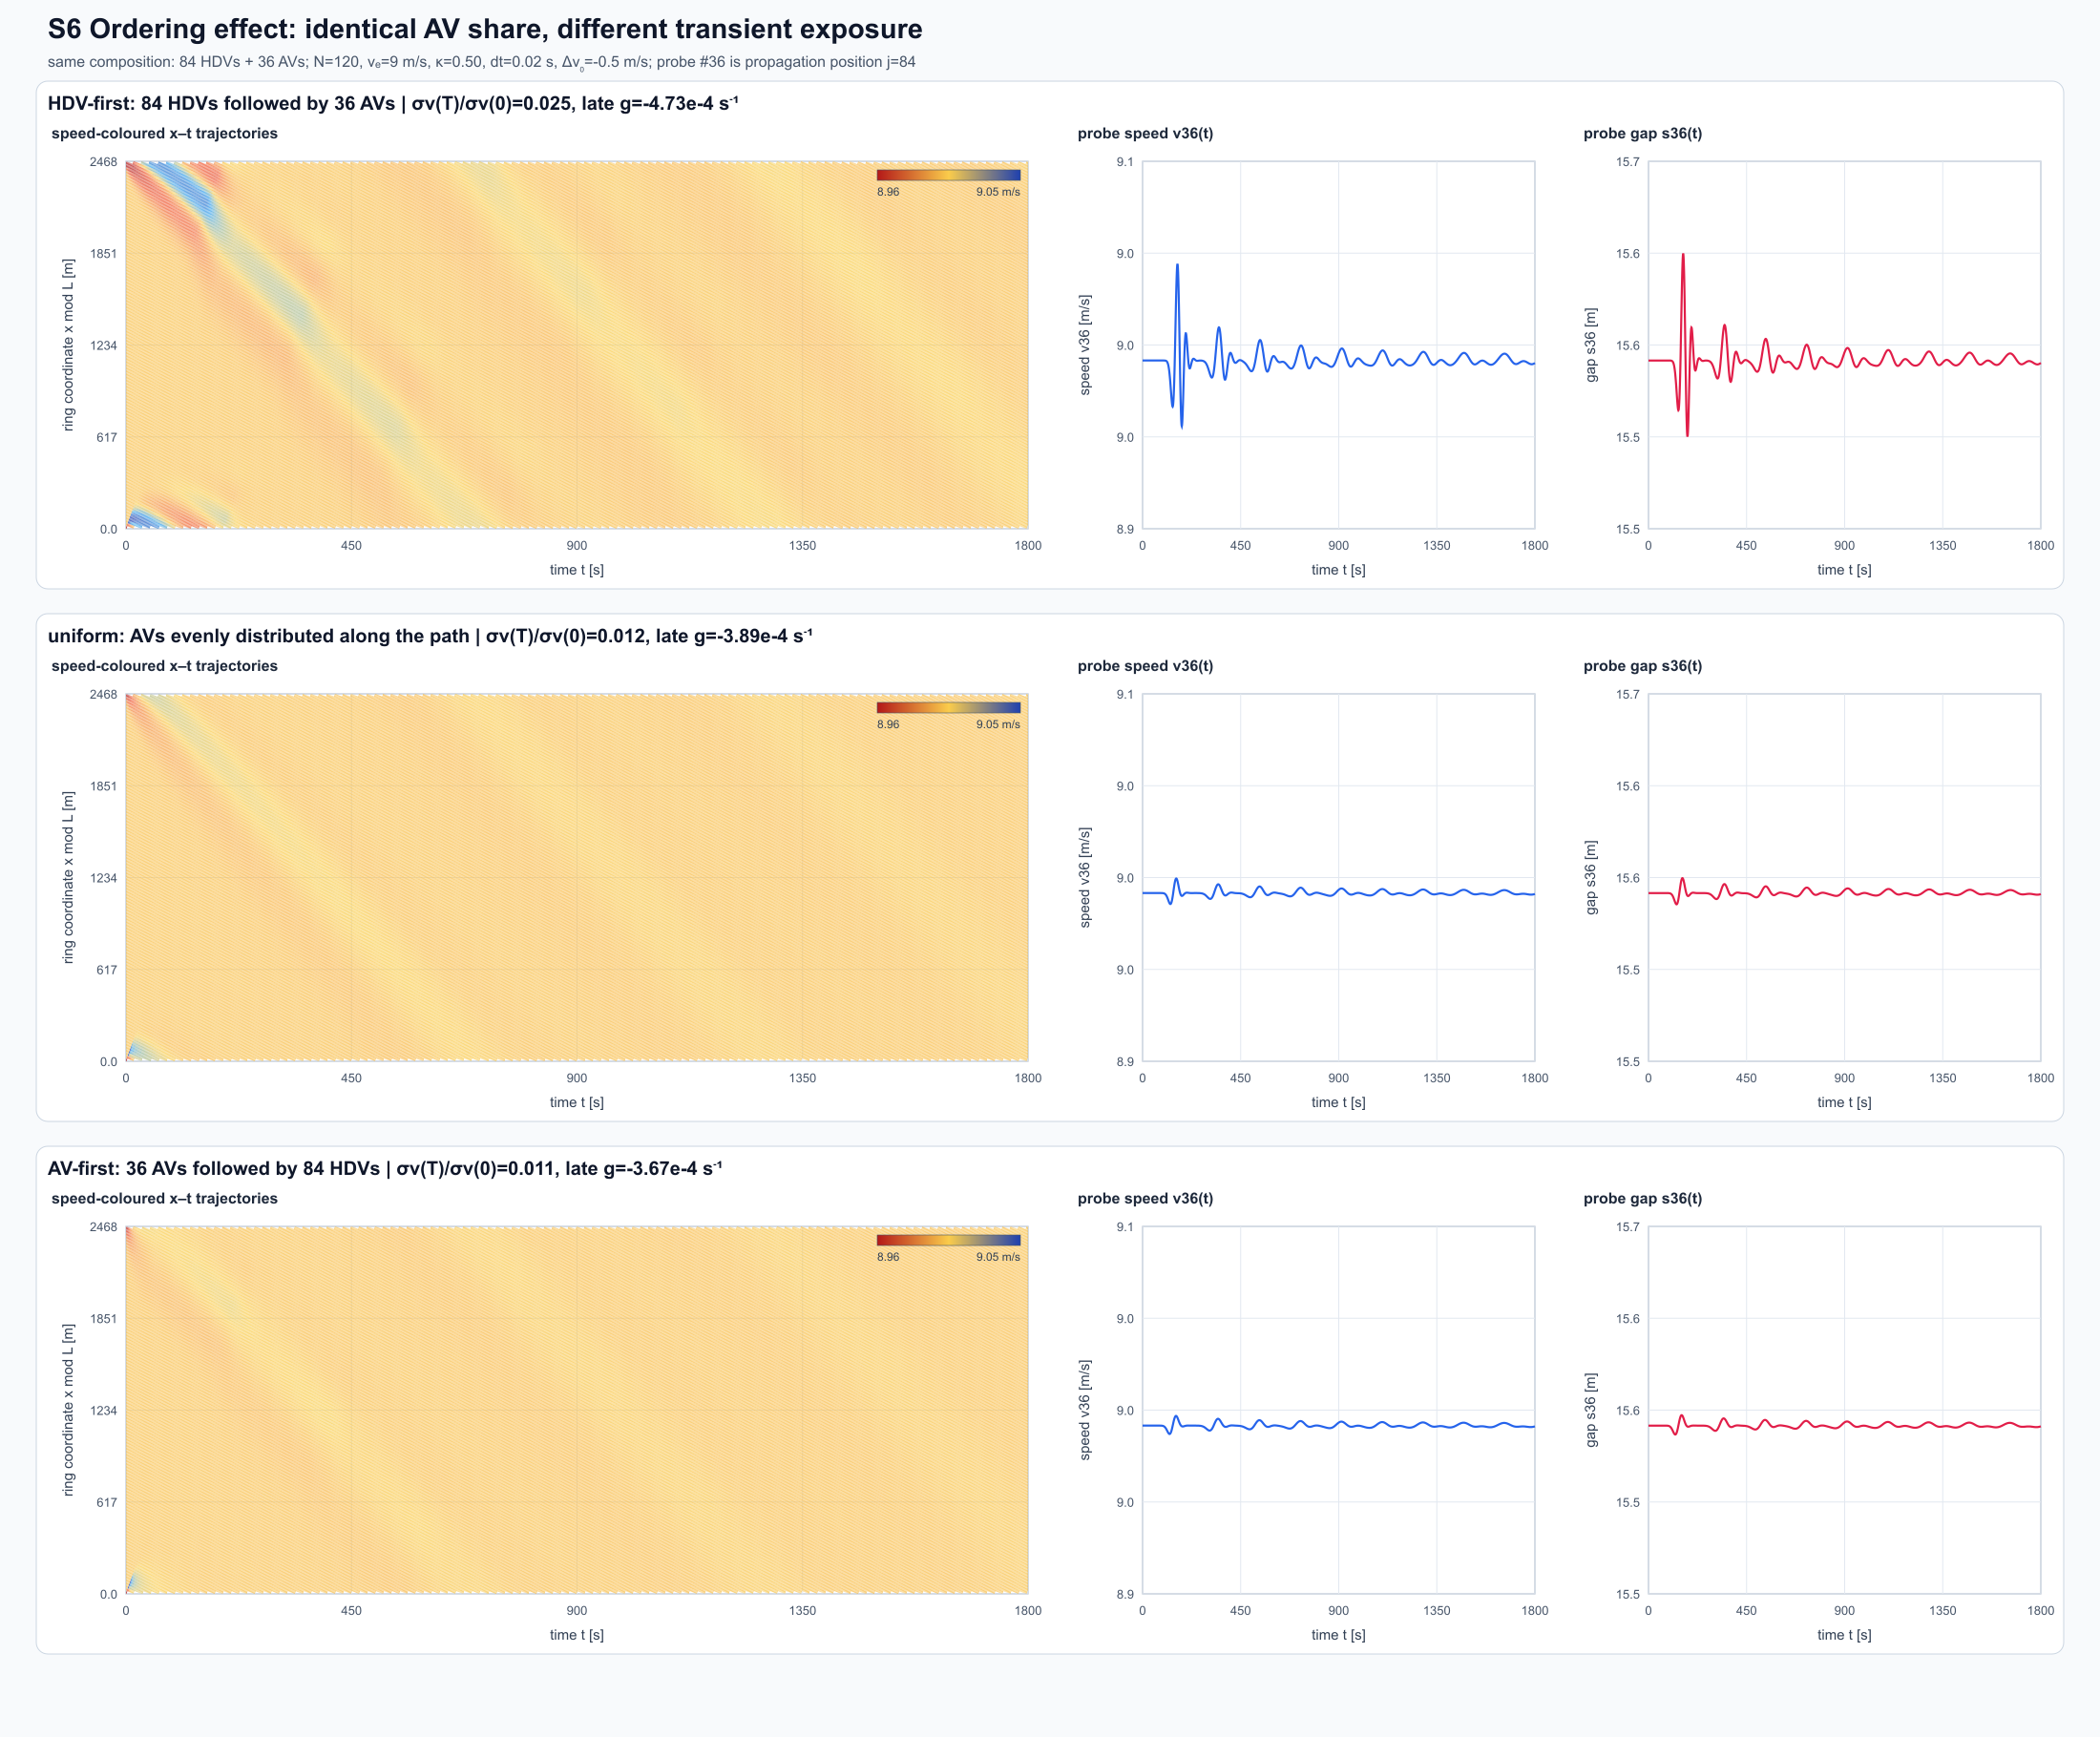
\includegraphics[width=\textwidth]{sim_s6_ordering_three.png}
\caption{S6：三种 AV/HDV 排序的时域对照。}
\label{fig:traj-s6}
\figurenote{S6 在相同车型配方下隔离排序效应。三行均含 84 辆 HDV 与 36 辆 AV，取相同 $v_e=9$ m/s、$\kappa=0.5$、$\Delta t=0.02$ s 和 $-0.5$ m/s 脉冲；从上到下依次让 HDV 位于传播路径前段、均匀交错以及 AV 位于输入端。左列使用共同色标，因此色带宽度和深浅可以直接比较：HDV 在前时扰动在遇到 AV 以前明显扩展，均匀排序不断插入衰减段，AV 在前则最早压制输入。右两列固定观察传播位置 $j=84$ 对应车辆，速度峰--峰值依次约为 0.0615、0.00968、0.00685 m/s，间距峰--峰值依次约为 0.104、0.0149、0.0110 m；差异远大于末态指标。三种方案最终标准差比都小于 0.026，证明总预算足以保证末端衰减；但途中峰值相差近一个数量级，证明排序决定局部车辆承受的速度和间距暴露。该图因此为图~\ref{fig:heter-order-budget} 的前缀和解释提供了完整非线性轨迹证据。}
\end{figure}

图~\ref{fig:traj-s7} 对应 E7：AV 跟随 HDV 时只能使用 $\kappa_0=0.15$，跟随 AV 时使用 $\kappa=0.5$。30\% AV 逐辆分散时，末段斜率为 $+1.61\times10^{-3}$ s$^{-1}$，$\sigma_v(1800)/\sigma_v(0)=1.672$；分成 4 个均匀编组后，末段斜率变为 $-3.37\times10^{-4}$ s$^{-1}$，首末比降至 $0.0273$。这给出了“同一渗透率，仅改变 AV--AV 邻接结构即可翻转稳定符号”的直接时域证据。

\begin{figure}[htbp]
\centering
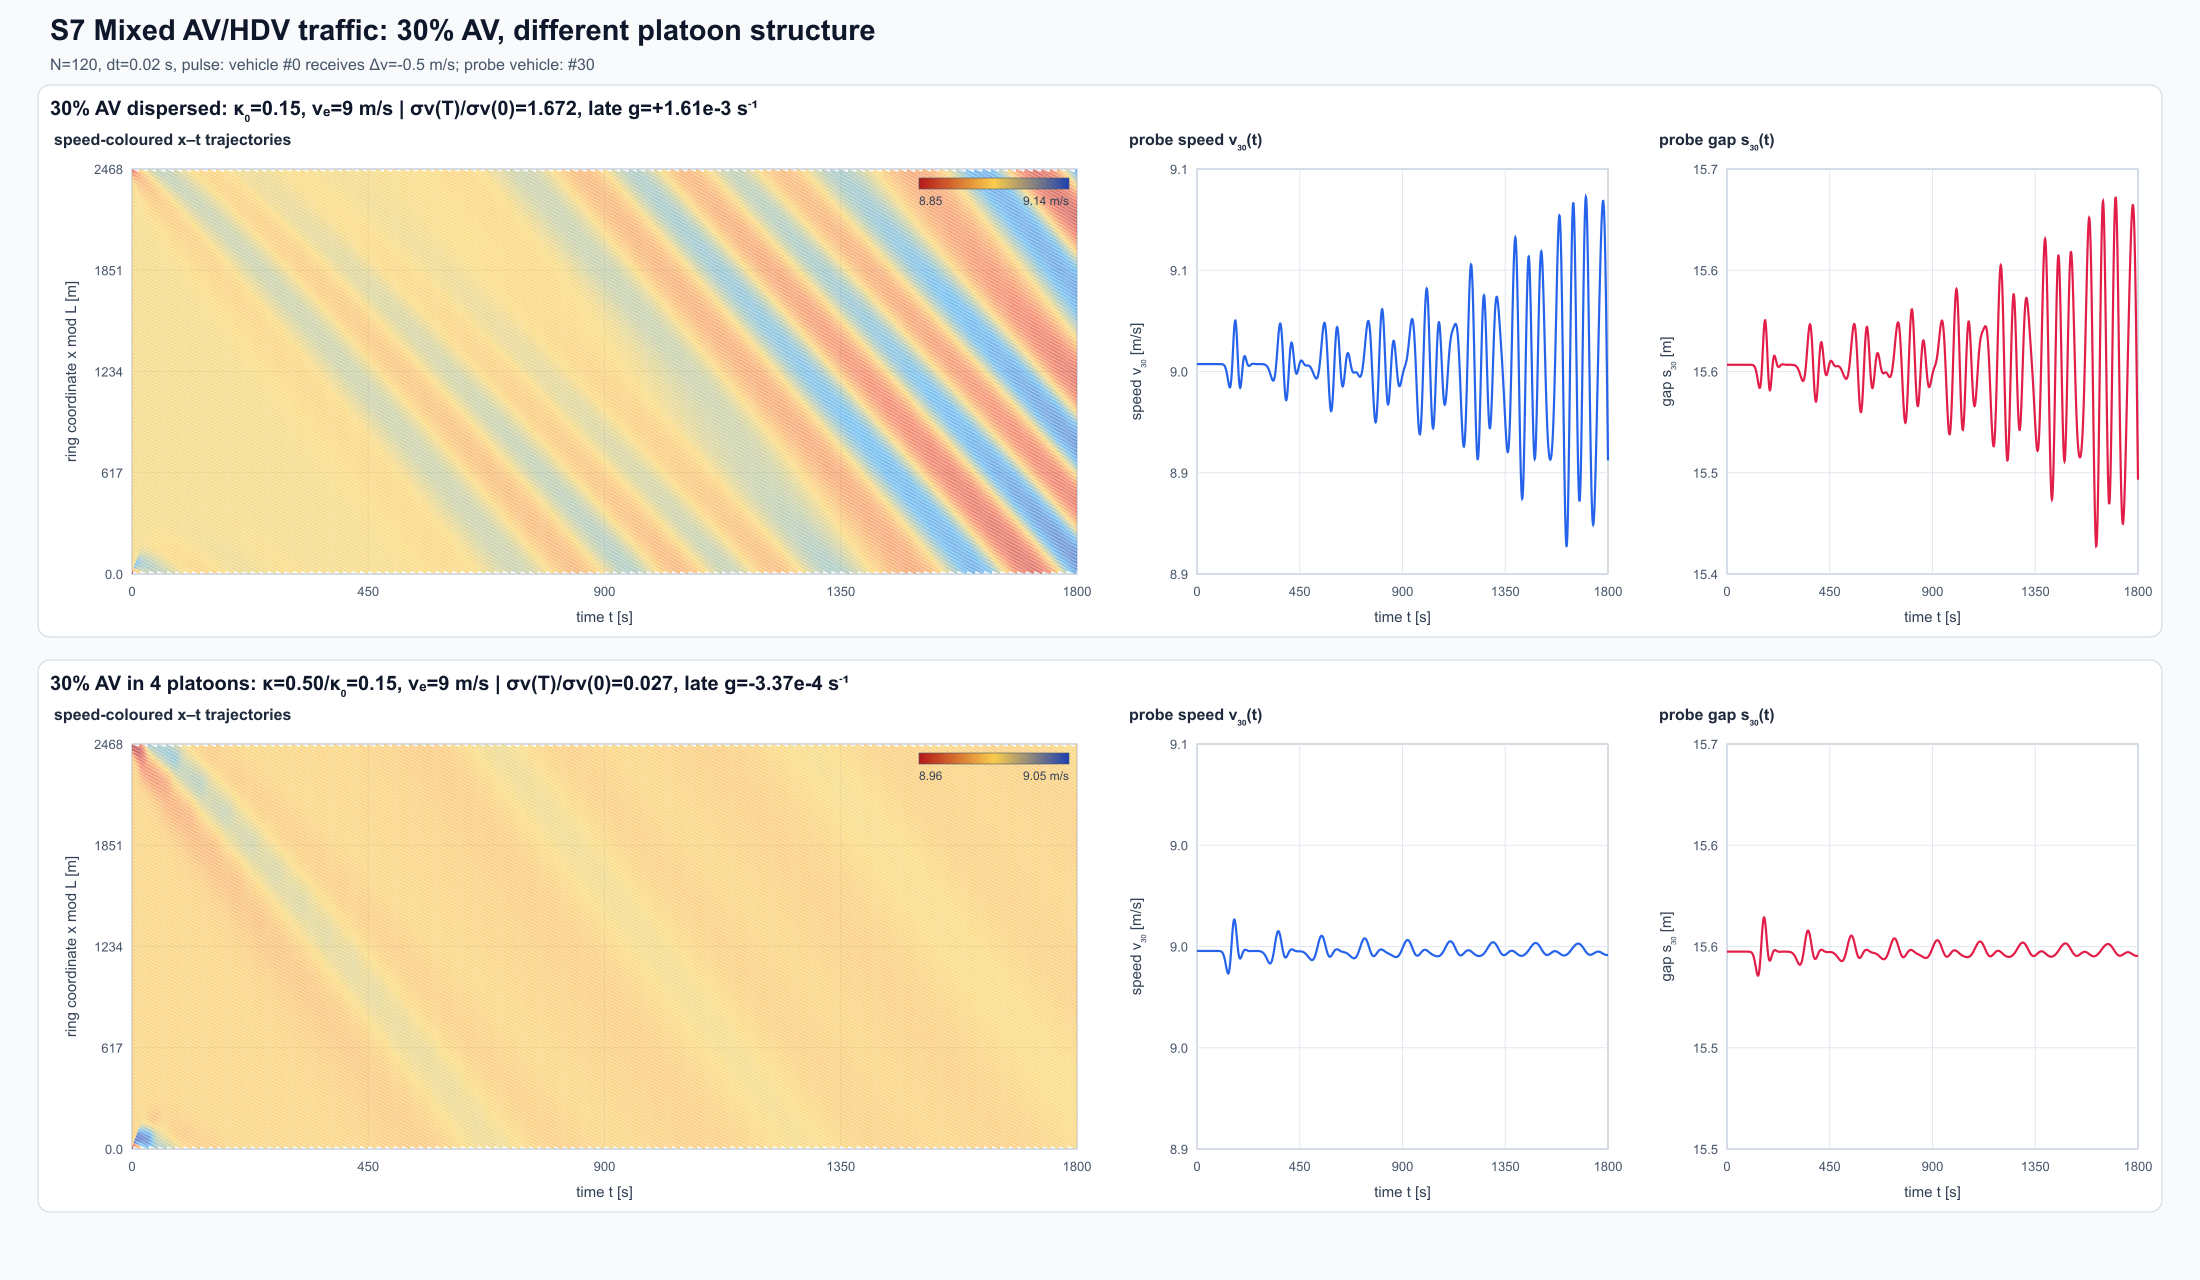
\includegraphics[width=\textwidth]{sim_s7_mixed_av.png}
\caption{S7：AV 编组结构的轨迹对照。}
\label{fig:traj-s7}
\figurenote{S7 说明相同 30\% AV 渗透率为何可能产生相反稳定结论。上行把 AV 逐辆分散，每辆 AV 的直接前车大多是 HDV，只能使用雷达估计增益 $\kappa_0=0.15$；下行把同样数量的 AV 分成 4 组，组内多数车辆可通过 V2V 使用 $\kappa=0.5$。上行位置--时间色带逐圈加深并形成持续波，第 30 辆车的速度和间距振幅同步增加；下行色带逐渐收窄，两个探针量回到平衡。因为车辆总数、AV 比例、工作点和扰动完全相同，差异只能来自 AV--AV 相邻对与实际可用增益，而不能归因于“更多 AV”。该图证明渗透率只是数量指标，通信拓扑才把数量转化为稳定预算，也解释了为什么混合交通设计必须同时报告排列与编组。}
\end{figure}

\sectionwrapup{异质车队的稳定性不仅取决于车型或 AV 渗透率，还取决于排列和相邻通信关系。相同 AV 比例下，分散布置与成组布置可以给出相反结论；宏观比例指标不能替代对具体拓扑的检验。}

%==================================================================
\PART{VII}{从微观线性门槛到非线性波、宏观模型与工程应用}

\chapter{原始 IDM 的弱非线性稳定性分析}
\label{sec:nonlinear}
\chapterguide{线性门槛之后，波幅与波形由什么决定}{本章比较线性、弱非线性与强非线性问题，推导 Gardner--Burgers 型正规形，并说明 Burgers、KdV、mKdV 与 Gardner 方程的适用条件及可观测证据。}

前文的线性理论回答“无穷小扰动起初增长还是衰减”，却不回答增长以后为什么不会无限发散、最终形成多大振幅和什么形状的走停波。本章只研究第~\ref{sec:idm}~章的\textbf{原始、均匀、单向、无延迟 IDM}，不把前馈、回望、异质性与延迟混入非线性约化，以免把不同机制的高阶项混在一起。

\section{非线性稳定性的目的：线性门槛之后还缺什么}
\sectionstudy{theory}{非线性稳定性的目的：线性门槛之后还缺什么}{komatsu1995,bando1995,ororsz2010}

“非线性稳定性”至少包含两个层次。严格的数学问题是：对一个有限但非零的初始扰动，解是否始终有界、是否回到均匀平衡，以及平衡态的吸引域有多大。弱非线性问题则更具体：在中性曲线附近，保留最低阶的平方、立方项后，线性增长如何被波形陡化、扩散和色散修正。本书完整讨论第二层，并用有限幅仿真探查第一层，但不把数值现象误称为全局证明。

线性谱只给出平衡态处的“切线信息”。它无法单独回答下面四个问题：
\begin{enumerate}[leftmargin=1.6em,itemsep=4pt]
\item \textbf{增长后会停在哪里？} $\operatorname{Re}\lambda>0$ 只预测初期指数增长；真实速度不会增长到无穷，而会形成有限幅走停波、停车平台或波峰并合。
\item \textbf{线性稳定是否足以抵抗大扰动？} $\operatorname{Re}\lambda<0$ 只保证足够小的扰动衰减。一次急刹车可能把系统推出小扰动邻域，产生很长的非线性暂态，甚至在存在亚临界分岔时落入另一吸引子。
\item \textbf{最终波形是什么？} 线性模态是正弦波叠加，不能决定波峰是否变尖、波谷是否形成停车平台，也不能给出孤波或 kink 的幅宽关系。
\item \textbf{控制器在拥堵已经形成后还能否消波？} 线性稳定化说明均匀态附近具有恢复方向；要判断现有 stop-and-go 是否会真正消失，还必须把当前有限幅状态作为初值直接积分，或研究受控系统的吸引域。
\end{enumerate}

\begin{tcolorbox}[keybox,title=\textbf{一句话区分}]
线性分析决定\textbf{均匀态附近的初始方向、时间尺度和主导波长}；非线性分析决定\textbf{有限幅扰动的阈值、饱和幅度、波形、传播速度修正及长期状态}。前者适合画“门槛”，后者适合解释“门槛之后发生什么”。
\end{tcolorbox}

\section{线性、弱非线性与强非线性各回答什么}
\sectionstudy{theory}{线性、弱非线性与强非线性各回答什么}{komatsu1995,bando1995,ororsz2010}

\begin{center}
\small
\captionof{table}{线性、弱非线性与完整非线性分析的分工。}
\label{tab:nonlinear-levels}
\begin{tabular}{p{3.1cm}p{5.2cm}p{5.4cm}}
\toprule
\textbf{层级} & \textbf{主要问题} & \textbf{适用范围／输出} \\
\midrule
线性谱分析 & 小扰动是否增长、哪一波长最快 & $|r|\to0$；输出 $\operatorname{Re}\lambda(k)$、$k^*$ 与中性曲线 \\[4pt]
弱非线性约化 & 靠近中性曲线时，波如何陡化、扩散与色散 & 小而缓变的有限幅波；输出 Burgers、KdV、mKdV 或 Gardner 振幅方程 \\[4pt]
完整非线性仿真 & 大幅减速、接近停车、波峰并合和长期吸引子 & 直接积分 IDM；输出有限幅时空轨迹，但一般没有简单闭式判据 \\
\bottomrule
\end{tabular}
\end{center}
\tabletext{tab:nonlinear-levels}{三种分析层级所回答的问题和适用范围。线性谱确定初始增长，弱非线性约化解释中性线附近的波形演化，完整仿真处理停车和波峰并合等强非线性现象。}

因此，$\Phi<0$ 只说明均匀态附近存在增长方向；它不意味着速度会按 $e^{\sigma t}$ 永远增长。随着振幅增大，IDM 的平方间距项、自由流项和接近率项共同改变瞬时恢复力，系统离开线性切平面，增长率随振幅变化并形成有限幅波。

还应区分\textbf{非线性方程}与\textbf{非线性稳定性结论}。直接写出完整 IDM 并不等于已经完成非线性稳定性分析；只有在给定扰动集合上证明恢复、计算吸引域边界、追踪分岔支，或系统扫描有限幅响应后，才能对非线性行为作出可检验的结论。

\section{常用方法：各自解决什么问题}
\sectionstudy{theory}{常用方法：各自解决什么问题}{komatsu1995,bando1995,ororsz2010}

\begin{center}
\small
\captionof{table}{非线性稳定性的常用方法及其适用边界。}
\label{tab:nonlinear-methods}
\begin{tabular}{p{3.0cm}p{5.0cm}p{5.7cm}}
\toprule
\textbf{方法} & \textbf{核心做法} & \textbf{最适合回答的问题／局限} \\
\midrule
多尺度／中心流形约化 & 在中性线附近引入慢空间、慢时间，把离散车队约化为振幅方程 & 得到 Burgers、KdV、mKdV、Gardner；可解释幅宽和波速修正，但只适用于小而缓变的波 \\[4pt]
能量或 Lyapunov 方法 & 构造随时间单调下降的函数，给出状态范数的上界 & 能提供严格的局部或全局充分条件；对含速度差、非对称耦合和饱和约束的 IDM 很难找到不保守的能量函数 \\[4pt]
分岔与数值延续 & 把密度、时距或增益当作参数，连续追踪平衡、周期波及其稳定性 & 识别超临界／亚临界分岔、共存吸引子和迟滞；计算成本高，且需直接处理环道相位平移零模态 \\[4pt]
有限幅直接仿真 & 扫描扰动幅值、波长和形状，长期积分完整 IDM & 最接近实验平台，可处理停车和波峰并合；只能对已扫描区域给出证据，不能替代全局证明 \\[4pt]
数据诊断 & 从轨迹拟合幅值方程、幅宽--速度关系和迟滞环 & 用于连接理论与实测；结果依赖观测窗、噪声、模态分离和初值覆盖 \\
\bottomrule
\end{tabular}
\end{center}
\tabletext{tab:nonlinear-methods}{多尺度、Lyapunov、分岔延续、直接仿真和数据诊断五类方法。它说明没有一种工具能够同时给出严格全局证明、闭式波形和真实大扰动响应，因此本书采用组合证据。}

本书采用“\textbf{线性谱定位中性点 $\rightarrow$ 多尺度约化解释机制 $\rightarrow$ 完整 IDM 有限幅仿真复核}”的组合。这样既保留了解析可读性，也避免把只在 $\varepsilon\ll1$ 下成立的约化方程外推到反复停车的强非线性区。

\section{典型交通场景：应选择哪一层分析}
\sectionstudy{theory}{典型交通场景：应选择哪一层分析}{komatsu1995,bando1995,ororsz2010}

\begin{center}
\small
\captionof{table}{典型交通场景与推荐的非线性分析工具。}
\label{tab:nonlinear-scenarios}
\begin{tabular}{p{3.5cm}p{4.7cm}p{5.5cm}}
\toprule
\textbf{场景} & \textbf{关键问题} & \textbf{推荐工具与观测量} \\
\midrule
接近中性线的小幅长波 & 波是缓慢衰减还是缓慢增长，波形为何逐渐变陡 & 线性谱 $+$ KdV--Burgers／Gardner；测 $\operatorname{Re}\lambda$、幅宽、相位速度 \\[4pt]
线性失稳后的走停波 & 指数增长何时饱和，最终停车频率和波幅多大 & 完整 IDM 长时仿真或周期波延续；测 $v_{\min}$、$v_{\max}$、$\sigma_v$ 和极限环 \\[4pt]
线性稳定下的急刹车 & 是否存在有限幅触发阈值或超长暂态 & 脉冲幅值扫描、双向参数扫描；测末窗能量、恢复时间和迟滞 \\[4pt]
两个拥堵波相遇 & 波峰合并、竞争还是相互穿透 & 强非线性仿真；追踪波峰位置、质量和合并时间 \\[4pt]
拥堵形成后打开 CACC & 控制能否把现有有限幅波拉回均匀态 & 切换系统仿真／吸引域分析；比较切换前后包络斜率与恢复时间 \\[4pt]
含换道、噪声或通信丢包 & 扰动持续被外部注入，确定性平衡不再封闭 & 随机稳定性、混杂系统或蒙特卡洛；测概率分布而非单条轨迹 \\
\bottomrule
\end{tabular}
\end{center}
\tabletext{tab:nonlinear-scenarios}{六类交通场景的关键问题、推荐工具和观测量。该表帮助读者根据扰动幅值、外部输入和是否存在切换选择分析层级，而不是对所有现象套用 mKdV。}

\section{从离散 IDM 到慢变振幅方程}
\sectionstudy{model}{从离散 IDM 到慢变振幅方程}{treiber2000,treiberkesting2013}

记间距与速度扰动为
\begin{equation}
r_n=s_n-s_e,
\qquad
u_n=v_n-v_e .
\end{equation}
不再把高阶项丢掉，而是在平衡点对完整 IDM 作 Taylor 展开：
\begin{equation}
\dot r_n=u_{n-1}-u_n,
\qquad
\dot u_n=\mathcal L_n(r,u)+\frac12\mathcal Q_n(r,u)+\frac16\mathcal C_n(r,u)+O(\|(r,u)\|^4),
\label{eq:nonlinear-taylor}
\end{equation}
其中 $\mathcal L_n$ 就是前文使用的线性算子，$\mathcal Q_n$、$\mathcal C_n$ 分别收集 IDM 二阶与三阶偏导产生的项。为了只观察跨越许多车辆的慢变波，引入
\begin{equation}
X=\varepsilon\bigl(n+c_1t\bigr),
\qquad
\mathcal T=\varepsilon^3t,
\qquad
c_1=V'(s_e),
\label{eq:slow-scales}
\end{equation}
这里 $\varepsilon$ 同时量化三个“小量”：波数 $k=O(\varepsilon)$、距离中性线的偏离以及扰动幅值。离散移位按
\begin{equation}
R(X\pm\varepsilon,\mathcal T)
=R\pm\varepsilon R_X+\frac{\varepsilon^2}{2}R_{XX}
\pm\frac{\varepsilon^3}{6}R_{XXX}+\cdots
\label{eq:nonlinear-shift-expansion}
\end{equation}
展开，所以 $R_X$ 给出长波平移，$R_{XX}$ 给出扩散／反扩散，$R_{XXX}$ 给出离散色散。推导可按四步理解：
\begin{enumerate}[leftmargin=1.6em,itemsep=3pt]
\item $O(\varepsilon)$：得到运动坐标的速度 $c_1=V'(s_e)$，它与线性长波相速一致；
\item $O(\varepsilon^2)$：得到系数 $c_2$，其符号就是长波稳定符号；
\item 再高一阶：二阶、三阶 Taylor 项分别产生 $RR_X$、$R^2R_X$，离散移位产生 $R_{XXX}$；
\item 消去随速度快速衰减的模态，并对慢模态施加可解性条件，得到单个标量振幅方程。
\end{enumerate}

把距离中性线的扩散系数写成 $c_2=O(\varepsilon)$。二次非线性占主导时取 $r_n=\varepsilon^2R(X,\mathcal T)+\cdots$；二次项退化、三次项主导时取 $r_n=\varepsilon R(X,\mathcal T)+\cdots$。逐阶消去快速速度松弛模态后，长波中心流形上的统一正规形为
\begin{tcolorbox}[keybox,title=\textbf{原始 IDM 的弱非线性长波正规形}]
\begin{equation}
R_{\mathcal T}
+\alpha_2 R R_X
+\alpha_3 R^2R_X
=\nu R_{XX}-\beta R_{XXX}+\text{高阶项},
\label{eq:gardner-burgers}
\end{equation}
\end{tcolorbox}
其中 $\nu$ 与线性长波系数 $c_2$ 同号，$\nu>0$ 表示耗散、$\nu<0$ 表示反扩散；$\beta$ 描述离散车队的色散；$\alpha_2$、$\alpha_3$ 分别控制二次与三次非线性陡化。变量缩放会同时改变这些系数的数值，但不会改变它们是否为零以及相对符号。

\begin{tcolorbox}[notebox,title=\textbf{约化成立的三个前提}]
必须同时满足：工作点靠近中性线、扰动幅值小、主导波长远大于车辆间距。若车辆已经停车、相邻间距接近 $s_0$，或者主导模态只有两三辆车一个波，则 $\varepsilon$ 不再小，式~\eqref{eq:gardner-burgers} 只能作定性解释，不能用来精确预测振幅。
\end{tcolorbox}

对以间距 $R$ 为振幅、并采用式~\eqref{eq:slow-scales} 的归一化，平衡流形给出的主导非线性系数为
\begin{equation}
\alpha_2=V''(s_e),
\qquad
\alpha_3=\frac12V'''(s_e).
\label{eq:nonlinear-coefficients}
\end{equation}
线性色散系数则由色散关系再展开一阶得到
\begin{align}
\lambda&=c_1\varepsilon+c_2\varepsilon^2+c_3\varepsilon^3+O(\varepsilon^4),
\qquad \varepsilon=-ik,\\
c_3&=\frac{(2c_1-f_{v_l})c_2-\frac12f_{v_l}c_1-\frac16f_s}{f_v+f_{v_l}}.
\label{eq:c3-general}
\end{align}
恰在中性线上 $c_2=0$，上式化为
\begin{equation}
c_3=\frac{f_s(2f_{v_l}-f_v)}{6(f_v+f_{v_l})^2}>0,
\qquad
\beta=c_3 .
\label{eq:c3-neutral}
\end{equation}
这说明在耗散项消失时，离散车辆结构留下的 $O(k^3)$ 相位修正不会同时消失，因而能够与非线性陡化平衡。

\section{Burgers、KdV、mKdV 和 Gardner 何时出现}
\sectionstudy{theory}{Burgers、KdV、mKdV 和 Gardner 何时出现}{komatsu1995,bando1995,ororsz2010}

式~\eqref{eq:gardner-burgers} 不是四个互不相关的模型，而是一个统一正规形在不同尺度下的退化：
\begin{center}
\small
\captionof{table}{Burgers、KdV、mKdV 与 Gardner 约化的主导平衡。}
\label{tab:reduced-wave-equations}
\begin{tabular}{p{2.5cm}p{5.5cm}p{5.8cm}}
\toprule
\textbf{约化} & \textbf{主导平衡} & \textbf{交通波含义} \\
\midrule
Burgers & $R_{\mathcal T}+\alpha_2RR_X=\nu R_{XX}$ & 非线性使波前变陡，正常扩散使其变宽；常见三角形／冲击型过渡 \\[4pt]
KdV & $R_{\mathcal T}+\alpha_2RR_X=-\beta R_{XXX}$ & 二次非线性与色散平衡；中性线附近可形成 $\operatorname{sech}^2$ 型孤立脉冲 \\[4pt]
mKdV & $R_{\mathcal T}+\alpha_3R^2R_X=-\beta R_{XXX}$，且 $\alpha_2=0$ & 三次非线性与色散平衡；按系数符号产生脉冲或 kink--antikink 波 \\[4pt]
Gardner & 二次、三次非线性同时保留 & $\alpha_2$ 很小但不严格为零时，比“纯 mKdV”更可靠 \\
\bottomrule
\end{tabular}
\end{center}
\tabletext{tab:reduced-wave-equations}{四种振幅方程的主导项与交通波含义。二次项是否退化、耗散与色散谁占主导，决定应使用哪一种约化形式。}

例如无耗散 KdV 在 $\alpha_2A/\beta>0$ 时有
\begin{equation}
R(X,\mathcal T)=A\,\operatorname{sech}^2\!\left(\frac{X-U\mathcal T}{L}\right),
\qquad
U=\frac{\alpha_2A}{3},
\qquad
L=\sqrt{\frac{12\beta}{\alpha_2A}}.
\label{eq:kdv-soliton}
\end{equation}
它给出一个可检验的幅宽关系 $L\propto|A|^{-1/2}$。mKdV 的 kink 解可写成
\begin{equation}
R(X,\mathcal T)=A\tanh\!\left(\frac{X-U\mathcal T}{L}\right),
\qquad
U=\frac{\alpha_3A^2}{3},
\qquad
L^2=-\frac{6\beta}{\alpha_3A^2},
\label{eq:mkdv-kink}
\end{equation}
但只有 $L^2>0$ 且两端状态满足守恒约束时才是实际可取的交通波。因而“看到一个陡峭波前”并不足以证明 mKdV；还应验证二次系数接近零、幅宽关系和传播速度。

\section{典型非线性现象及其可观测证据}
\sectionstudy{theory}{典型非线性现象及其可观测证据}{komatsu1995,bando1995,ororsz2010}

\begin{description}[style=unboxed,leftmargin=0pt,labelindent=0pt,labelsep=0.5em,itemsep=0.65em,font=\normalfont\bfseries\color{navy}]
\item[波形陡化]
同一波的上升沿或下降沿越来越窄，高次空间谐波随时间增强。它说明传播速度依赖局部振幅，是 $RR_X$ 或 $R^2R_X$ 的直接表现。

\item[非线性饱和]
早期 $\ln|A(t)|$ 近似直线，随后斜率下降，$\sigma_v$ 在有限水平附近波动。此时不能再用一个固定 $\lambda$ 拟合全过程。

\item[孤立波与 kink]
孤立波是局部脉冲；kink 连接两个不同平台。判断不能只凭外形，还应检验传播速度随 $A$ 或 $A^2$ 变化，以及 $L\propto|A|^{-1/2}$ 或 $L\propto|A|^{-1}$ 的缩放。

\item[亚临界触发与迟滞]
同一参数下，小扰动回到均匀流，大扰动却长期保持波动；从均匀态增大密度与从拥堵态减小密度得到不同转变点。必须用双向扫描和足够长的观测窗确认。

\item[恢复时间的振幅依赖]
即使最终都回到平衡，大扰动也可能比线性时间尺度慢很多。工程上“1800 s 内仍有波动”与“数学上永不衰减”不是同一句话。
\end{description}

图~\ref{fig:nonlinear-five-observables} 把上述五种现象转换成实验台中可直接操作或读取的观测量。这里必须区分两类图：图~\ref{fig:nonlinear-five-observables}(a)、(b)、(d)、(e) 来自完整 IDM 数值积分；图~\ref{fig:nonlinear-five-observables}(c) 是 KdV/mKdV 约化方程的形状与缩放模板，用来说明“怎样检验”，并不是声称基准 IDM 已经产生严格 mKdV kink。

\begin{figure}[htbp]
\centering
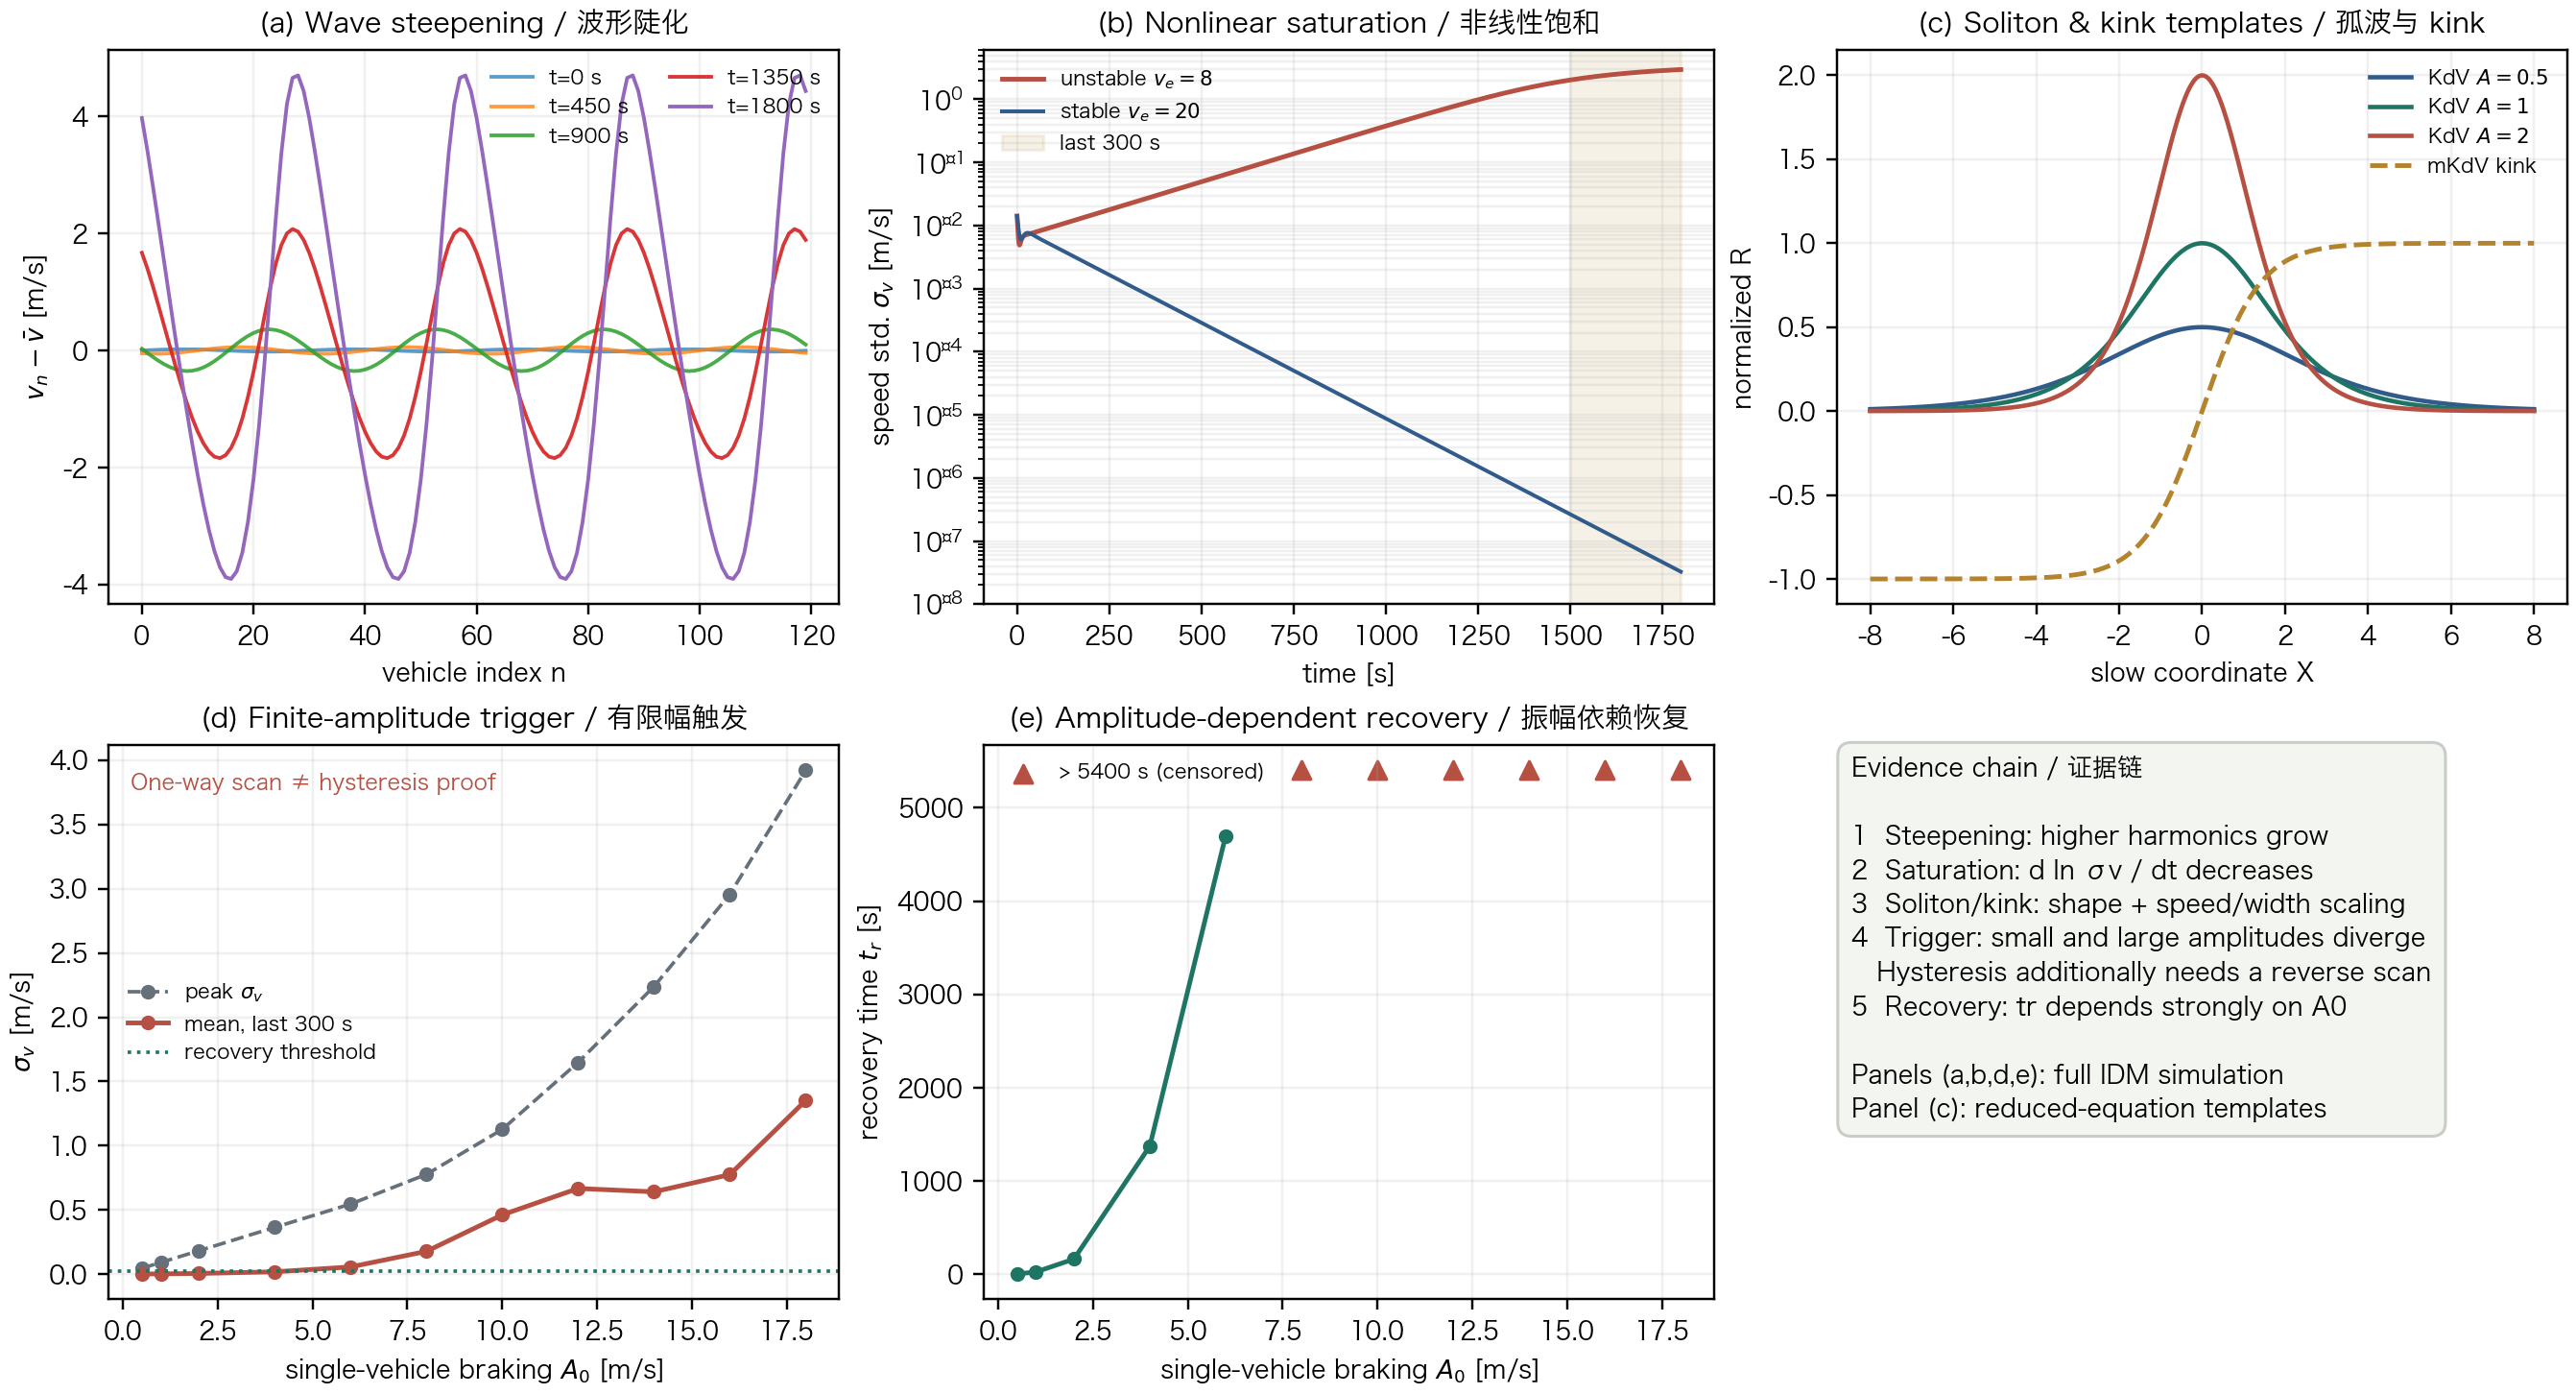
\includegraphics[width=\textwidth]{nonlinear_phenomena_observables.png}
\caption{五类非线性现象的可观测证据。}
\label{fig:nonlinear-five-observables}
\figurenote{五类非线性稳定现象及其各自需要的观测证据。第一面板比较基波与高次谐波：波峰变尖、波谷变宽以及高次谱能量上升证明波形已不再服从单一线性模态。第二面板把早期指数包络与后期平台并列，显示正线性增长率只预测初始放大，最终振幅由非线性饱和决定。第三面板将数值波形与 KdV/mKdV 类约化模板比较，用传播速度和形状保持性判断孤立波近似是否成立；第四面板扫描初始扰动幅值，寻找线性稳定点是否存在有限幅触发阈值。第五面板报告恢复时间，三角形表示 5400 s 内仍未达到标准的右删失案例，避免把“尚未恢复”误写成一个虚假的精确时间。整图证明线性稳定性只能回答无穷小扰动的早期趋势，波形、饱和、阈值和恢复速度必须依靠非线性指标分别判断。}
\end{figure}

\begin{center}
\small
\captionof{table}{五类非线性现象的观测量与本算例证据。}
\label{tab:nonlinear-observables}
\begin{tabular}{p{2.7cm}p{4.4cm}p{6.1cm}}
\toprule
\textbf{现象} & \textbf{平台中的观测量} & \textbf{本算例的具体结果与正确结论} \\
\midrule
波形陡化 & 速度空间剖面；高次谐波比 $H=\sqrt{\sum_{m\ge8}|\hat v_m|^2}/|\hat v_4|$ & $H$ 在 $t=0,450,900,1350,1800$ s 分别为 $0,0.0034,0.0213,0.1091,0.1903$，说明波形逐步偏离单一正弦模态。 \\[3pt]
非线性饱和 & $\log\sigma_v$--$t$ 曲线的瞬时斜率；末窗均值 & $v_e=8$ m/s 时 $\sigma_v$ 由 $0.01414$ 增至 $2.962$ m/s，末 300 s 均值为 $2.554$ m/s；后段弯折表明固定线性增长率已不适用，但末时仍缓慢增长，故只称“进入饱和区”。 \\[3pt]
孤立波／kink & 波形、传播速度和幅宽随振幅的缩放 & KdV 模板满足 $L\propto |A|^{-1/2}$，mKdV kink 模板满足 $L\propto |A|^{-1}$；只有外形而没有缩放与系数退化检查，不能认定为孤波或 kink。 \\[3pt]
有限幅触发／迟滞 & 同一工况的幅值扫描；均匀态／拥堵态双向扫描 & 在 $v_e=20$ m/s 处，$A_0=0.5$ m/s 的末窗 $\sigma_v=8.8\times10^{-4}$ m/s，而 $A_0=18$ m/s 为 $1.351$ m/s，证明强幅值依赖；但单向扫描不能证明迟滞，迟滞仍需双向初值扫描。 \\[3pt]
振幅依赖恢复 & 首次连续 300 s 满足 $\sigma_v<0.02$ m/s 的时间 $t_r$ & $A_0=0.5,2,4,6$ m/s 时 $t_r=4,164,1374,4700$ s；$A_0\ge8$ m/s 到 5400 s 仍未达阈值，只能报告为右删失。 \\
\bottomrule
\end{tabular}
\end{center}
\tabletext{tab:nonlinear-observables}{波形陡化、饱和、孤波模板、有限幅触发和恢复时间的可观测证据。每一行同时给出能支持的结论和不能越界声称的内容，防止只凭波形相似作模型判定。}

\begin{tcolorbox}[notebox,title=\textbf{怎样在实验台中使用这五张图}]
选择“非线性现象”页签后，五个按钮对应图~\ref{fig:nonlinear-five-observables} 的五类证据。波形陡化可以拖动剖面时刻；孤波／kink 可以拖动模板振幅并观察幅宽缩放；其余三项显示同一组长时 IDM 扫描结果、具体数值和结论边界。这样读者既能看到现象，也能知道哪一项是完整 IDM 证据、哪一项只是约化方程模板，以及哪些数据仍不足以证明迟滞。
\end{tcolorbox}

\section{原始 IDM 是否真的满足 mKdV 条件}
\sectionstudy{model}{原始 IDM 是否真的满足 mKdV 条件}{treiber2000,treiberkesting2013}

IDM 的平衡曲线由 $s_e=s_e(v_e)$ 显式给出，因此无需对隐函数反复求导：
\begin{equation}
V'=\frac{1}{s_e'(v_e)},
\qquad
V''=-\frac{s_e''(v_e)}{[s_e'(v_e)]^3},
\qquad
V'''=\frac{3[s_e''(v_e)]^2}{[s_e'(v_e)]^5}-\frac{s_e'''(v_e)}{[s_e'(v_e)]^4}.
\label{eq:inverse-derivatives}
\end{equation}
对本书基准参数作高精度中心差分，得到：
\begin{center}
\small
\captionof{table}{基准 IDM 在三个工作点的弱非线性系数。}
\label{tab:idm-nonlinear-coefficients}
\begin{tabular}{p{2.8cm}rrrr}
\toprule
工况 & $V'$ & $V''$ & $V'''$ & $c_3$ \\
 & [s$^{-1}$] & [m$^{-1}$s$^{-1}$] & [m$^{-2}$s$^{-1}$] & [veh$^3$/s] \\
\midrule
下中性边界 $v_e\approx0.91$ & $0.666665$ & $-5.12\times10^{-6}$ & $-9.49\times10^{-6}$ & $0.1938$ \\
失稳工况 $v_e=8$ & $0.660405$ & $-1.997\times10^{-3}$ & $-4.676\times10^{-4}$ & $1.8942$ \\
上中性边界 $v_e\approx18.61$ & $0.514195$ & $-1.474\times10^{-2}$ & $-4.13\times10^{-4}$ & $1.1446$ \\
\bottomrule
\end{tabular}
\end{center}
\tabletext{tab:idm-nonlinear-coefficients}{两个中性边界与一个失稳点的 $V'$、$V''$、$V'''$ 和色散系数。下边界的 $V''$ 很小但不严格为零，因此更适合 Gardner 近似，而不能无条件称为纯 mKdV。}

\begin{tcolorbox}[resultbox,title=\textbf{关于 mKdV 的具体结论}]
基准 IDM 在两个中性边界都没有满足严格的 $V''(s_e)=0$，所以\textbf{不能把纯 mKdV 当作整个原始 IDM 的通用非线性方程}。下边界的 $|V''|$ 极小，间距振幅达到约 $1$ m 时二次项 $|V''R|$ 与三次项 $|V'''R^2/2|$ 已同量级，因此该处适合用 Gardner 方程描述“近 mKdV”行为；上边界的二次系数明显不为零，更接近 KdV／KdV--Burgers 情形。这个数值检查避免了把文献中针对特定最优速度函数的 mKdV 结论未经条件检验地直接套到 IDM 上。
\end{tcolorbox}

\section{E11：1800 s 有限幅试验与弱非线性解释}
\sectionstudy{experiment}{E11：1800 s 有限幅试验与弱非线性解释}{komatsu1995,bando1995,ororsz2010}
\label{sub:nonlinear-exp}

取 $N=120$、$\Delta t=0.05$ s、RK4 和 1800 s 时间窗。第一组在均匀平衡态上注入 $m=4$、速度振幅 $0.02$ m/s 的正弦扰动；第二组在小扰动线稳定的 $v_e=20$ m/s 工况中，只让一辆车瞬间减速 $0.5$--$18$ m/s，检查有限幅恢复。

\begin{figure}[htbp]
\centering
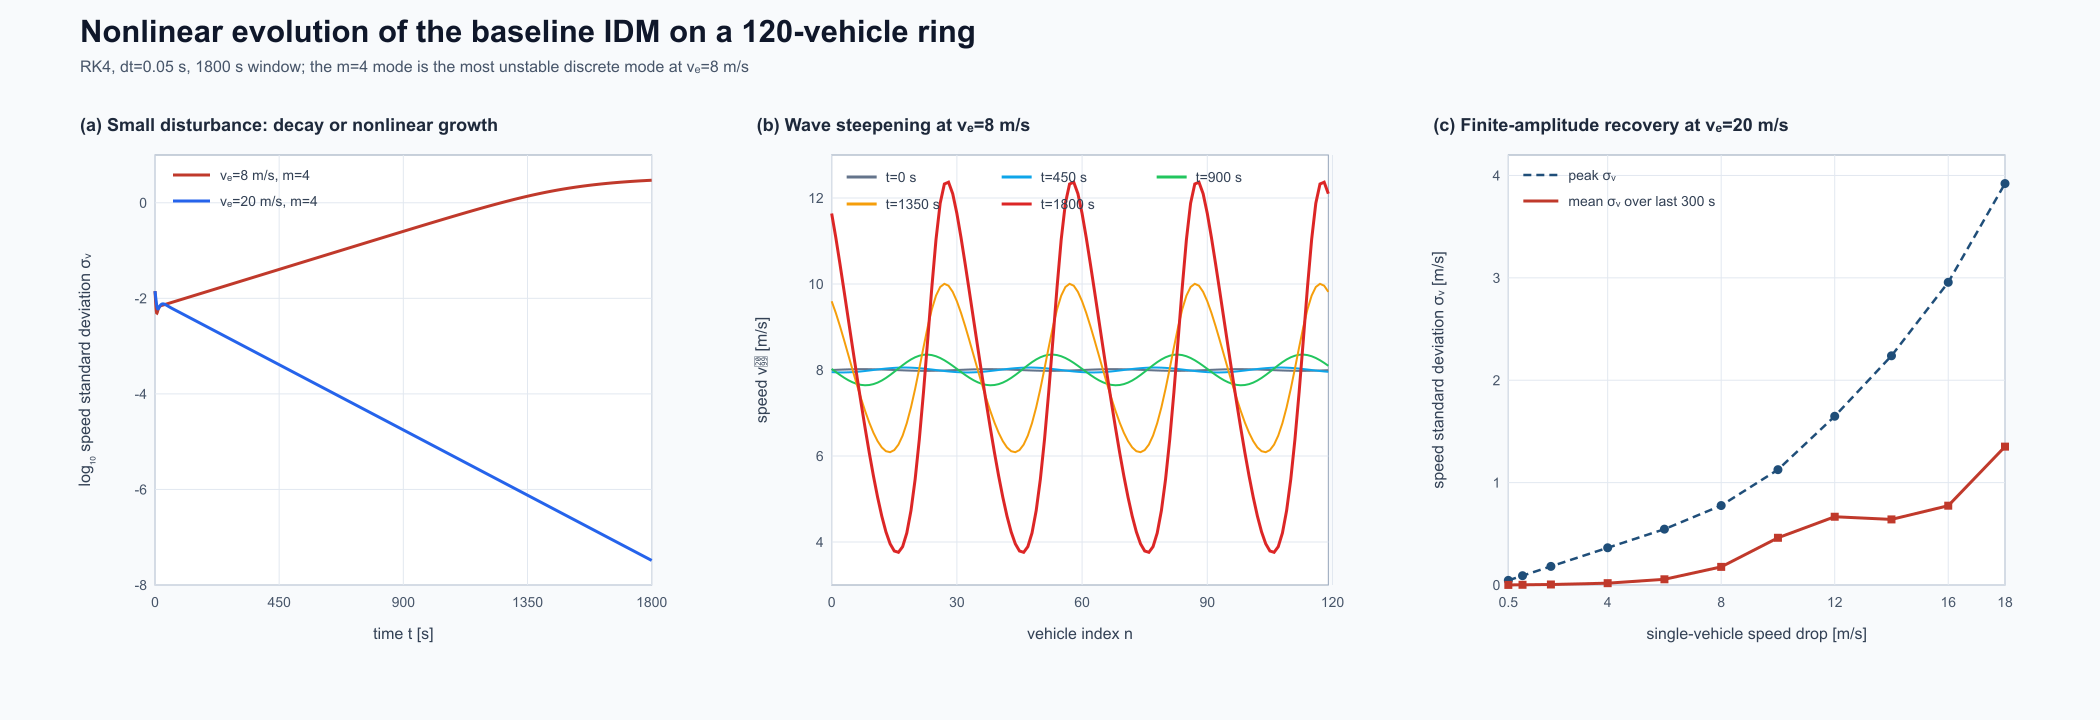
\includegraphics[width=\textwidth]{nonlinear_idm_experiment.png}
\caption{原始 IDM 的非线性演化与有限幅响应。}
\label{fig:nonlinear-idm}
\figurenote{原始 IDM 的线性预测与有限幅非线性结局。左图比较 $v_e=8$ 和 20 m/s 的主导模态包络：失稳工况早期沿线性正增长率直线上升，随后偏离指数并进入有限平台；稳定工况则持续下降，说明非线性没有改变小扰动的初始稳定符号。中图沿失稳工况截取不同时刻的空间波形，最初近似正弦，随后前后坡度不对称并出现高次结构，证明模态相互作用和波形陡化已经发生。右图在名义线性稳定点逐级增加单车制动幅值，同时画出全过程峰值和末 300 s 残余；二者分离说明大瞬时响应不等于持续失稳，而残余突然抬升才是有限幅吸引域变化的证据。该图证明线性理论可靠地描述早期指数阶段，但无法单独给出最终走停波振幅、有限幅阈值或恢复时间。}
\end{figure}

\begin{center}
\small
\captionof{table}{E11 原始 IDM 的 1800 s 有限幅结果。}
\label{tab:e11-nonlinear}
\begin{tabular}{p{4.0cm}p{4.3cm}p{5.4cm}}
\toprule
\textbf{算例} & \textbf{1800 s 结果} & \textbf{解释} \\
\midrule
$v_e=8$ m/s，$m=4$，$A_0=0.02$ m/s & $\sigma_v:0.01414\to2.962$ m/s；末时速度 $3.76$--$12.37$ m/s & 线性不稳定先选择 $m=4$，随后非线性使波形陡化；末段不能再用固定 $\lambda$ 拟合 \\[5pt]
$v_e=20$ m/s，同一小扰动 & $\sigma_v:0.01414\to3.27\times10^{-8}$ m/s & 与 $\Phi=+2.833\times10^{-3}>0$ 一致，小扰动恢复 \\[5pt]
$v_e=20$ m/s，单车减速 $18$ m/s & 全程峰值 $3.921$ m/s；最后 300 s 平均 $1.351$ m/s & 线性稳定不等于“有限时间内迅速恢复”；大扰动产生长暂态，需继续延长时间窗才能区分慢衰减与持久波 \\
\bottomrule
\end{tabular}
\end{center}
\tabletext{tab:e11-nonlinear}{线性失稳小扰动、线性稳定小扰动和稳定点大脉冲三种算例。结果把初期线性增长、后期波形陡化和大扰动长暂态区分开来。}

\begin{tcolorbox}[notebox,title=\textbf{这组实验能证明什么、不能证明什么}]
它证明线性谱能够预测\textbf{初始增长符号和最先出现的模态}，而弱非线性项解释了随后发生的波形陡化与幅值依赖。它不构成全局 Lyapunov 稳定性证明，也不能仅凭 1800 s 内仍有残余波动就断言存在亚临界第二吸引子。若要研究亚临界性，应对每个脉冲至少延长到多个衰减时间常数，并分别从均匀态与拥堵态作双向参数扫描，检查迟滞。
\end{tcolorbox}

\section{E12：线性稳定工况的有限幅响应图}
\sectionstudy{experiment}{E12：线性稳定工况的有限幅响应图}{komatsu1995,bando1995,ororsz2010}

为把“线性稳定”和“对大扰动恢复得快”分开，在 $v_e=20$ m/s、$N=120$ 的线性稳定工况中，仅改变 0 号车的瞬时减速幅值 $A_0$，其余参数与 E11 相同。下表给出全过程最大速度标准差和最后 300 s 的平均速度标准差：
\begin{center}
\small
\captionof{table}{E12 不同制动幅值下的全过程峰值与末窗残余。}
\label{tab:e12-finite-amplitude}
\begin{tabular}{rccccc}
\toprule
$A_0$ [m/s] & 0.5 & 4 & 8 & 12 & 18 \\
\midrule
$\max_t\sigma_v$ [m/s] & 0.0455 & 0.3636 & 0.7762 & 1.6483 & 3.9211 \\
末 300 s 平均 $\sigma_v$ [m/s] & 0.00088 & 0.01777 & 0.17705 & 0.66670 & 1.35145 \\
\bottomrule
\end{tabular}
\end{center}
\tabletext{tab:e12-finite-amplitude}{同一线性稳定工作点在五种单车减速幅值下的响应。小脉冲几乎完全恢复，大脉冲末窗仍有显著波动，说明线性稳定不等于有限时间内对任意幅值快速恢复。}

小脉冲在 1800 s 内几乎完全消失，与线性稳定结论一致；随着 $A_0$ 增大，末窗残余非线性波动快速上升。进一步把积分延长到 5400 s，并定义恢复时间为首次连续 300 s 满足 $\sigma_v<0.02$ m/s，可得
\begin{equation}
t_r(A_0=0.5,2,4,6\ {\rm m/s})=(4,164,1374,4700)\ {\rm s}.
\label{eq:nonlinear-recovery-times}
\end{equation}
当 $A_0\ge8$ m/s 时，5400 s 内仍未达到该阈值，故只能记为 $t_r>5400$ s 的\textbf{右删失}结果，而不能记成 $t_r=\infty$。对 $A_0=4,6$ m/s 用 $\Delta t=0.10$ s 和 $0.05$ s 重算，二者都得到 $1374$ s 和 $4700$ s，说明这里的巨大恢复时间不是由所用步长制造的。该扫描给出的可靠结论是“恢复时间和暂态幅值强烈依赖扰动幅值”，而不是“$A_0=18$ m/s 已证明存在永久拥堵”。要把后者变成结论，还需继续积分并从波动态反向扫描参数寻找迟滞。

\begin{tcolorbox}[resultbox,title=\textbf{E11--E12 的线性／非线性对照}]
\begin{itemize}[leftmargin=1.4em,itemsep=3pt]
\item $v_e=8$ m/s：线性谱先正确预测小扰动增长和主导模态；非线性项随后决定波形陡化与有限幅饱和。
\item $v_e=20$ m/s、$A_0=0.02$ m/s：线性理论足以预测快速恢复。
\item $v_e=20$ m/s、大制动脉冲：稳定符号没有改变，但线性化严重低估恢复时间和峰值；必须直接积分完整 IDM。
\end{itemize}
因此，非线性分析不是用来“推翻”线性判据，而是为线性判据补上适用半径、有限幅后果和长期吸引状态。
\end{tcolorbox}

\section{非线性分析的实际使用顺序}
\sectionstudy{synthesis}{非线性分析的实际使用顺序}{komatsu1995,bando1995,ororsz2010}

\begin{enumerate}[leftmargin=1.6em,itemsep=4pt]
\item 先用线性谱确定中性边界、$k^*$ 与线性时间尺度 $1/|\operatorname{Re}\lambda|$；若这一层不对，后续非线性拟合没有可信基准。
\item 在中性线附近计算 $V''$、$V'''$ 与 $c_3$：$V''$ 明显非零用 KdV--Burgers；$V''\approx0$ 时保留三次项并优先用 Gardner；只有 $V''=0$ 的退化点才使用纯 mKdV。
\item 用多组初始幅值验证缩放律：线性阶段增长率应与幅值无关；KdV 孤波应近似满足 $L\propto|A|^{-1/2}$；mKdV kink 应满足 $L\propto|A|^{-1}$。
\item 一旦车辆接近停车、间距接近 $s_0$ 或加速度达到强非线性区，停止用弱非线性方程外推，返回完整 IDM 仿真。
\end{enumerate}

%==================================================================
\sectionwrapup{线性稳定性只描述无穷小扰动的初始增长率；弱非线性分析进一步给出波形陡化、有限幅饱和与恢复时间。对 IDM，可靠做法是先用线性谱定位阈值，再在阈值附近选择 KdV--Burgers、mKdV 或 Gardner 约化，最后用完整非线性仿真验证有限幅结论。}

\chapter{宏观交通流模型}
\label{sec:macro-models}
\chapterguide{把车辆看成连续流体后，方程从哪里来}{本章从控制体车辆守恒出发，依次推导 LWR、PW 与 ARZ 的闭合结构，解释物质导数、松弛、交通压力、黏性和广义速度的来源，并给出有限体积求解流程。}

微观模型逐车计算 $x_n(t)$ 和 $v_n(t)$；宏观模型则在固定道路位置 $x$ 上描述密度 $\rho(x,t)$、空间平均速度 $v(x,t)$ 与流量
\begin{equation}
q(x,t)=\rho(x,t)v(x,t).
\label{eq:macro-fields}
\end{equation}
它把许多车辆组成的离散系统近似为连续介质。这里先回答“宏观方程从哪里来”，下一章才回答“这些方程的均匀解是否稳定”。

\section{共同起点：固定控制体上的车辆守恒}
\sectionstudy{theory}{共同起点：固定控制体上的车辆守恒}{helbing2001,leveque2002,treiberkesting2013}

取固定路段 $[x_1,x_2]$。若无匝道源汇，路段内车辆数
\begin{equation}
N(t)=\int_{x_1}^{x_2}\rho(x,t)\,\mathrm dx
\end{equation}
的变化只可能来自上游流入与下游流出：
\begin{equation}
\frac{\mathrm d}{\mathrm dt}\int_{x_1}^{x_2}\rho\,\mathrm dx
=q(x_1,t)-q(x_2,t)
=-\int_{x_1}^{x_2}q_x\,\mathrm dx .
\label{eq:macro-integral-conservation}
\end{equation}
由于控制区间任意，被积函数必须逐点满足
\begin{equation}
\boxed{\rho_t+q_x=0,\qquad q=\rho v.}
\label{eq:macro-continuity-intro}
\end{equation}
将乘积展开还可写成
\begin{equation}
\rho_t+v\rho_x+\rho v_x=0.
\label{eq:continuity-expanded}
\end{equation}
式~\eqref{eq:macro-continuity-intro} 只表达“车辆不会凭空产生或消失”，却有 $\rho$ 和 $v$ 两个未知场，因此还需要一个\textbf{闭合关系}。LWR、PW 和 ARZ 的本质差别，正是它们如何闭合速度。

\section{基本图：只描述平衡，不描述恢复过程}
\sectionstudy{model}{基本图：只描述平衡，不描述恢复过程}{helbing2001,leveque2002,treiberkesting2013}

均匀交通达到平衡时，用速度--密度关系和流量--密度关系表示为
\begin{equation}
v=V(\rho),\qquad Q(\rho)=\rho V(\rho).
\label{eq:macro-fundamental-diagram-intro}
\end{equation}
通常 $V'(\rho)<0$，而 $Q(\rho)$ 先增后减。基本图回答“给定密度最终希望以多快行驶”，但不回答“需要多长时间恢复”，更不单独决定扰动增长率。同一条 $Q(\rho)$ 可以配上不同松弛时间或压力闭合，得到完全不同的动态稳定性。本书后续不用独立的 Greenshields 曲线，而由 IDM 平衡关系生成 $V(\rho)$，使宏观平衡态与微观平衡态一致。

\section{LWR：守恒律加瞬时平衡闭合}
\sectionstudy{theory}{LWR：守恒律加瞬时平衡闭合}{lighthill1955,richards1956,leveque2002}

LWR 的关键假设是：局部速度没有独立惯性，密度一旦改变，速度立即取平衡值 $v=V(\rho)$。把它代入车辆守恒便得到\cite{lighthill1955,richards1956}
\begin{equation}
\boxed{\rho_t+\bigl[Q(\rho)\bigr]_x=0,\qquad Q(\rho)=\rho V(\rho).}
\label{eq:lwr-model-derivation}
\end{equation}
这里的下标 $x$ 表示对道路位置求偏导，$\bigl[Q(\rho)\bigr]_x$ 不是
$Q(\rho)$ 与 $x$ 相乘。由于密度本身是 $\rho=\rho(x,t)$，流量实际是复合函数
$Q(\rho(x,t))$。对光滑解使用链式法则：
\begin{equation}
\frac{\partial}{\partial x}Q\!\left(\rho(x,t)\right)
=\frac{\mathrm dQ}{\mathrm d\rho}
\frac{\partial\rho}{\partial x}
=Q'(\rho)\rho_x.
\label{eq:lwr-chain-rule-detail}
\end{equation}
因此式~\eqref{eq:lwr-model-derivation} 等价于
\begin{equation}
\rho_t+Q'(\rho)\rho_x=0.
\label{eq:lwr-characteristic-form}
\end{equation}
例如取抛物线基本图
\begin{equation}
Q(\rho)=v_f\rho\left(1-\frac{\rho}{\rho_j}\right),
\qquad
Q'(\rho)=v_f\left(1-\frac{2\rho}{\rho_j}\right),
\label{eq:lwr-example-flux}
\end{equation}
则局部密度波的传播速度是
$c(\rho)=Q'(\rho)$。低密度时 $Q'>0$，波通常向下游传播；高密度支上
$Q'<0$，即使车辆仍向下游行驶，拥堵波也可向上游传播。这里的
$Q'(\rho)$ 是\textbf{运动学波速}，不是车辆速度 $V(\rho)$。

这一解释可由特征线严格写出。沿任意道路曲线 $x=x(t)$，密度的全导数为
\begin{equation}
\frac{\mathrm d\rho}{\mathrm dt}
=\rho_t+\frac{\mathrm dx}{\mathrm dt}\rho_x.
\label{eq:lwr-density-total-derivative}
\end{equation}
选择
\begin{equation}
\frac{\mathrm dx}{\mathrm dt}=Q'(\rho),
\label{eq:lwr-characteristic-speed-detail}
\end{equation}
再使用式~\eqref{eq:lwr-characteristic-form}，便有
\begin{equation}
\frac{\mathrm d\rho}{\mathrm dt}
=\rho_t+Q'(\rho)\rho_x=0.
\end{equation}
所以密度值沿速度为 $Q'(\rho)$ 的特征线保持不变。若后方特征追上前方特征，光滑波会压缩成激波。

\begin{tcolorbox}[notebox,title=\textbf{为什么还必须保留守恒形式？}]
从 $\bigl[Q(\rho)\bigr]_x$ 写成 $Q'(\rho)\rho_x$ 只对连续可微的密度场成立。激波处 $\rho$ 跳跃，$\rho_x$ 不再是普通函数，此时必须回到
\[
\rho_t+\bigl[Q(\rho)\bigr]_x=0
\]
的守恒形式，在弱解意义下跨越激波积分。连接左右状态 $\rho_L,\rho_R$ 的激波速度不是简单代入某个 $Q'(\rho)$，而由 Rankine--Hugoniot 条件确定。
\end{tcolorbox}
跨越激波对式~\eqref{eq:lwr-model-derivation} 积分，得到 Rankine--Hugoniot 速度
\begin{equation}
s_{\rm sh}
=\frac{Q(\rho_R)-Q(\rho_L)}{\rho_R-\rho_L}.
\label{eq:lwr-rh-model}
\end{equation}
因此 LWR 很适合计算排队边界、激波速度和稀疏波，但“瞬时平衡”意味着它没有独立的速度恢复模态，也不能从模型内部产生跟驰扰动逐车放大的机制。

\subsection{手算例 W02：四个 LWR 网格怎样更新两步}
\label{sub:worked-lwr}

先用一个便于手算的三角形基本图演示有限体积更新：
\begin{equation}
Q(\rho)=\min\{30\rho,\;5(0.15-\rho)\},
\label{eq:w02-triangular-fd}
\end{equation}
其中密度单位为 veh/m、流量单位为 veh/s。临界密度为
$21.4286$ veh/km，容量为 $0.642857$ veh/s，即 $2314.3$ veh/h。
取四个单元、$\Delta x=500$ m、$\Delta t=5$ s，并固定左右虚拟单元密度为
$10$ 与 $50$ veh/km。初值为
\begin{equation}
\bm\rho^0=(10,20,50,50)\ {\rm veh/km}.
\label{eq:w02-initial}
\end{equation}
对三角形图，Godunov 通量可写为
\[
\widehat Q(\rho_L,\rho_R)=\min\{D(\rho_L),S(\rho_R)\},
\]
其中 $D$ 是上游需求、$S$ 是下游供给。五个界面从左到右的第一步通量为
\begin{equation}
\widehat{\bm Q}^{\,0}=(0.3,0.3,0.5,0.5,0.5)\ {\rm veh/s}.
\label{eq:w02-first-flux}
\end{equation}
例如第二个单元的流入为 $0.3$、流出为 $0.5$ veh/s，因此
\begin{align}
\rho_1^1
&=0.020-\frac{5}{500}(0.5-0.3)
=0.018\ {\rm veh/m}
=18\ {\rm veh/km}.
\label{eq:w02-cell-update}
\end{align}
四个单元同时更新后
\[
\bm\rho^1=(10,18,50,50)\ {\rm veh/km}.
\]
用 $\bm\rho^1$ 重新计算界面通量，再推进一步得到
\begin{equation}
\bm\rho^2=(10,16,50,50)\ {\rm veh/km}.
\label{eq:w02-second-update}
\end{equation}
第二个单元每 5 s 减少 2 veh/km，是因为它持续以 $0.3$ veh/s 接收车辆，
却以 $0.5$ veh/s 向拥堵区供给车辆。整个更新只使用“流入减流出”，这正是
守恒形式的离散含义；不能直接在跳跃处用 $Q'(\rho)\rho_x$ 作中心差分。

\subsection{教学算例 M06：IDM 基本图上的可核对激波}
\label{sub:m06-lwr}

W02 为了手算采用三角形图；M06 则换回本书的 IDM 平衡基本图。在 4 km 道路上
取左、右密度 $20$ 与 $60$ veh/km，Rankine--Hugoniot 条件给出
\begin{equation}
c_{\rm sh}=\frac{Q(60)-Q(20)}{60-20}
=-2.42536\ {\rm m/s}.
\label{eq:m06-shock}
\end{equation}
用 $\Delta x=25$ m、$\Delta t=0.5$ s 的 Godunov 法推进 60 s，
按密度中值定位得到 $-2.29167$ m/s；绝对误差为 $0.13370$ m/s，
小于一个网格位置对应的 $\Delta x/60=0.4167$ m/s。

\begin{figure}[htbp]
\centering
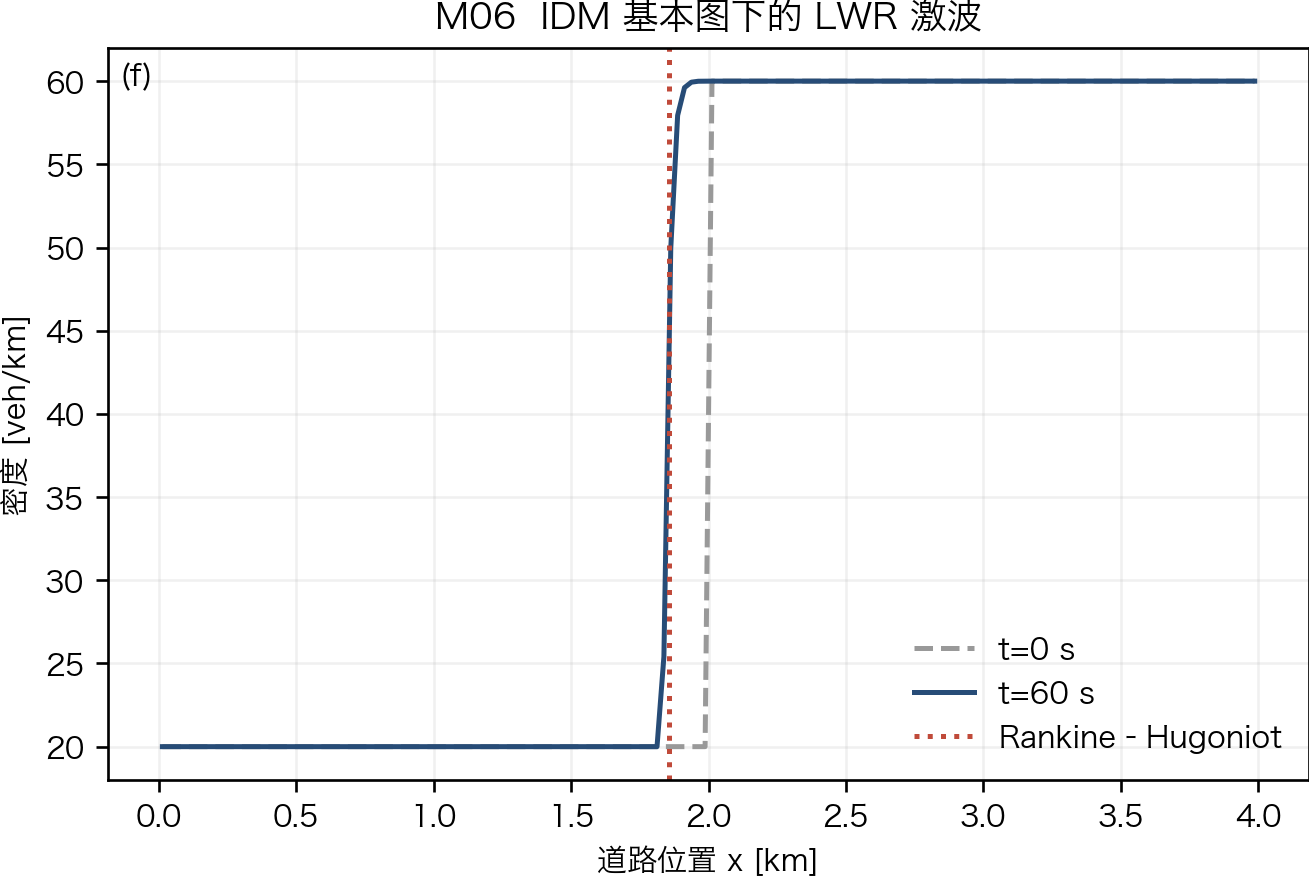
\includegraphics[width=0.84\textwidth]{mini_example_m06.png}
\caption{M06：IDM 基本图下的 LWR 激波。}
\label{fig:m06-lwr}
\figurenote{M06 用最小 LWR 网格验证守恒更新和激波速度。初始道路由两个不同 IDM 平衡密度状态组成，有限体积法在每个界面按流入减流出更新；蓝色曲线是若干网格分辨率下 60 s 的数值密度剖面，红色位置由 Rankine--Hugoniot 公式 $c_s=(q_R-q_L)/(\rho_R-\rho_L)$ 独立预测。随着网格细化，数值跃迁区围绕同一个红色位置收窄，说明扩散主要来自离散通量，而激波传播速度由车辆守恒正确保持。计算得到的 $c_s<0$ 表示密度间断在固定道路坐标中向上游移动，车辆本身仍以正速度向下游行驶。该图证明宏观时空图中的逆向拥堵波不需要假设车辆倒车，而是不同密度状态之间的守恒边界运动。}
\end{figure}

\section{PW：为速度加入惯性、压力和松弛}
\sectionstudy{theory}{PW：为速度加入惯性、压力和松弛}{payne1971,daganzo1995,jin2003}

要描述车辆速度不能瞬时跳到 $V(\rho)$，需把 $v$ 也作为状态。PW 的结构确实受到一维可压缩 Euler／Navier--Stokes 方程启发，但它不是车辆的真实机械动量守恒，而是一个\textbf{流体类比下的行为闭合}。

\subsection{物质导数：跟着车辆观察到的实际加速度}

设一辆车辆的轨迹为 $x=x(t)$，且
\begin{equation}
\frac{\mathrm dx}{\mathrm dt}=v(x(t),t).
\end{equation}
车辆实际经历的速度是复合函数 $v(x(t),t)$。链式法则给出
\begin{align}
\frac{\mathrm d}{\mathrm dt}v(x(t),t)
&=\frac{\partial v}{\partial t}
+\frac{\mathrm dx}{\mathrm dt}\frac{\partial v}{\partial x}\\
&=v_t+vv_x.
\end{align}
因此跟随车流移动的观察者看到的速度变化是物质导数
\begin{equation}
\frac{\mathrm Dv}{\mathrm Dt}=v_t+vv_x.
\label{eq:material-derivative}
\end{equation}
这里 $v_t$ 是固定检测器看到的局部时间变化，$vv_x$ 则是车辆驶入不同速度区域产生的对流变化。即使速度场不随时间变化（$v_t=0$），车辆进入一个下游速度逐渐降低的区域（$v_x<0$）时，仍有 $\mathrm Dv/\mathrm Dt=vv_x<0$，会实际减速。

\subsection{方程结构来自哪里：与一维可压缩 NS 的对应}

一维可压缩流体的质量和动量方程可写成
\begin{subequations}
\label{eq:ns-analogy}
\begin{align}
\rho_t+(\rho u)_x&=0,\\
(\rho u)_t+(\rho u^2+p)_x
&=(\mu u_x)_x+\rho f,
\end{align}
\end{subequations}
其中 $u$ 是流体速度，$p$ 是压力，$\mu$ 是动力黏度，$f$ 是单位质量外力。利用第一式展开第二式并消去质量守恒项，可得
\begin{equation}
u_t+uu_x
=-\frac{1}{\rho}p_x
+\frac{1}{\rho}(\mu u_x)_x+f.
\label{eq:ns-nonconservative}
\end{equation}
在局部均匀密度附近，可把 $\mu/\rho$ 合并为近似常数 $\nu$，右侧黏性项便写成 $\nu u_{xx}$。PW 用交通速度 $v$ 替代 $u$，用交通压力 $P(\rho)$ 替代机械压力 $p$，再把“外力”换成驾驶者主动追赶平衡速度的松弛作用。于是得到“物质加速度 $=$ 松弛 $-$ 压力梯度 $+$ 黏性”的结构\cite{payne1971}：
\begin{equation}
\boxed{
\frac{\mathrm Dv}{\mathrm Dt}
=\frac{V(\rho)-v}{\tau}
-\frac{1}{\rho}P_x
+\nu v_{xx}.}
\label{eq:pw-force-balance}
\end{equation}
若去掉黏性和松弛，结构更接近可压缩 Euler；保留黏性时接近 Navier--Stokes；再加入松弛项后才成为交通流 PW 模型。

\subsection{三类作用的交通含义与近似来源}

\paragraph{松弛：主动加速或制动。}
最简单的恢复律是
\begin{equation}
\frac{\mathrm dv}{\mathrm dt}
=\frac{V(\rho)-v}{\tau}.
\label{eq:pw-relaxation-alone}
\end{equation}
若短时间内把 $\rho$ 视为常数，则
\begin{equation}
v(t)=V(\rho)+\bigl[v(0)-V(\rho)\bigr]e^{-t/\tau}.
\end{equation}
所以 $v<V(\rho)$ 时车辆加速，$v>V(\rho)$ 时车辆减速，$\tau$ 是偏差衰减的时间尺度。该项不是标准 NS 方程固有的力，而是交通行为额外加入的主动驱动／制动项。

\paragraph{交通压力：对前方密度梯度的预见。}
假设驾驶者观察前方距离 $d$ 处的密度。对光滑场作 Taylor 展开：
\begin{align}
\rho(x+d,t)
&=\rho(x,t)+d\rho_x+O(d^2),\\
V\!\left(\rho(x+d,t)\right)
&=V(\rho)+dV'(\rho)\rho_x+O(d^2).
\end{align}
正常交通中 $V'(\rho)<0$。若前方越来越拥挤，即 $\rho_x>0$，第二个修正项为负，车辆应提前减速。PW 把这类预见统一写成
\begin{equation}
-\frac{1}{\rho}P_x
=-\frac{P'(\rho)}{\rho}\rho_x,
\label{eq:pw-pressure-chain}
\end{equation}
其中 $P'(\rho)>0$。因此 $\rho_x>0$ 时该项为负，$\rho_x<0$ 时为正。“交通压力”不是车辆之间的真实接触压力，而是密度梯度引起的预见响应。

\paragraph{黏性：邻近速度差的平滑。}
若局部驾驶状态受到两侧邻域平均速度
\begin{equation}
\bar v(x)=\frac{v(x+d)+v(x-d)}{2}
\end{equation}
的影响，Taylor 展开给出
\begin{equation}
\bar v-v
=\frac{d^2}{2}v_{xx}+O(d^4).
\end{equation}
令调整项为 $\gamma(\bar v-v)$，即可写成
\begin{equation}
\gamma(\bar v-v)\simeq
\underbrace{\frac{\gamma d^2}{2}}_{\nu}v_{xx}
=\nu v_{xx}.
\label{eq:pw-viscosity-average}
\end{equation}
速度局部峰值处 $v_{xx}<0$，黏性使其下降；速度谷值处 $v_{xx}>0$，黏性使其上升。因此它平滑速度差并抑制很短的波。这个对称平均也暴露了 PW 的气体式特征：真实驾驶主要看前方，而不是前后完全对称。

\subsection{从物质导数组装 PW 方程}

因为 $P=P(\rho)$，有 $P_x=P'(\rho)\rho_x$。将式~\eqref{eq:material-derivative} 代入式~\eqref{eq:pw-force-balance}：
\begin{equation}
v_t+vv_x
=\frac{V(\rho)-v}{\tau}
-\frac{P'(\rho)}{\rho}\rho_x
+\nu v_{xx}.
\end{equation}
把压力项移到左边，并与独立的车辆守恒式合并，得到
\begin{subequations}
\label{eq:pw-model-derivation}
\begin{align}
\rho_t+(\rho v)_x&=0,\\
v_t+vv_x+\frac{P'(\rho)}{\rho}\rho_x
&=\frac{V(\rho)-v}{\tau}+\nu v_{xx}.
\end{align}
\end{subequations}
\begin{tcolorbox}[keybox,title=\textbf{式~\eqref{eq:material-derivative} 与 PW 方程的逻辑关系}]
式~\eqref{eq:material-derivative} 只是“车辆实际加速度如何由速度场计算”的运动学恒等式，并不能单独推出 PW。式~\eqref{eq:pw-force-balance} 才是关于驾驶响应的建模假设；将二者结合得到速度方程，再与车辆守恒联立，才形成闭合的二阶 PW 系统。
\end{tcolorbox}
常系数压力取 $P'(\rho)=c_0^2$，其中 $c_0$ 控制密度梯度引起的预见强度。若去掉松弛与黏性，齐次系统的特征速度为 $v-c_0$ 与 $v+c_0$。第二个速度大于车辆速度，意味着某些信息可向车辆前方传播；这正是经典 PW 被批评为具有“气体式”各向同性的原因\cite{daganzo1995}。PW 的价值仍然很大：它把惯性、压力、松弛怎样共同产生增长或衰减展示得最直接。

\section{ARZ：从各向异性的广义速度推导}
\sectionstudy{theory}{ARZ：从各向异性的广义速度推导}{awrascle2000,zhang2002}

Aw--Rascle--Zhang（ARZ）模型不是直接给 $v$ 加对称压力，而定义广义速度
\begin{equation}
w=v+p(\rho),\qquad p'(\rho)>0,
\label{eq:arz-generalized-velocity-model}
\end{equation}
并假设 $w$ 随车辆运动而输运，同时通过松弛把实际速度拉回基本图\cite{awrascle2000,zhang2002}：
\begin{subequations}
\label{eq:arz-model-derivation}
\begin{align}
\rho_t+(\rho v)_x&=0,\\
w_t+vw_x&=\frac{V(\rho)-v}{\tau}.
\end{align}
\end{subequations}

\subsection{从广义速度到速度形式：链式法则逐项展开}

式~\eqref{eq:arz-generalized-velocity-model} 中
$w(x,t)=v(x,t)+p(\rho(x,t))$。由于 $p$ 的自变量是密度，而密度又依赖 $x,t$，分别对时间和位置求偏导时必须使用复合函数链式法则：
\begin{subequations}
\label{eq:arz-chain-components}
\begin{align}
w_t
&=\frac{\partial v}{\partial t}
+\frac{\mathrm dp}{\mathrm d\rho}
\frac{\partial\rho}{\partial t}
=v_t+p'(\rho)\rho_t,\\
w_x
&=\frac{\partial v}{\partial x}
+\frac{\mathrm dp}{\mathrm d\rho}
\frac{\partial\rho}{\partial x}
=v_x+p'(\rho)\rho_x.
\end{align}
\end{subequations}
第二式乘以交通速度 $v$：
\begin{equation}
vw_x=vv_x+vp'(\rho)\rho_x.
\end{equation}
再与 $w_t$ 相加：
\begin{align}
w_t+vw_x
&=v_t+p'(\rho)\rho_t+vv_x+vp'(\rho)\rho_x\\
&=v_t+vv_x+p'(\rho)\bigl(\rho_t+v\rho_x\bigr).
\label{eq:arz-chain-expanded}
\end{align}
因此原来简写的一步就是
\begin{equation}
w_t+vw_x
=v_t+vv_x+p'(\rho)\bigl(\rho_t+v\rho_x\bigr).
\label{eq:arz-material-chain}
\end{equation}

也可以把它看成物质导数的链式法则：
\begin{equation}
\frac{\mathrm Dw}{\mathrm Dt}
=\frac{\mathrm Dv}{\mathrm Dt}
+p'(\rho)\frac{\mathrm D\rho}{\mathrm Dt},
\qquad
\frac{\mathrm D}{\mathrm Dt}
=\frac{\partial}{\partial t}
+v\frac{\partial}{\partial x}.
\label{eq:arz-material-compact}
\end{equation}
这与式~\eqref{eq:arz-chain-expanded} 完全相同。

下一步使用车辆守恒。将
$\rho_t+(\rho v)_x=0$ 的乘积展开：
\begin{equation}
\rho_t+v\rho_x+\rho v_x=0
\quad\Longrightarrow\quad
\rho_t+v\rho_x=-\rho v_x.
\label{eq:arz-continuity-substitution}
\end{equation}
代入式~\eqref{eq:arz-chain-expanded}：
\begin{align}
w_t+vw_x
&=v_t+vv_x-\rho p'(\rho)v_x\\
&=v_t+\bigl[v-\rho p'(\rho)\bigr]v_x.
\label{eq:arz-speed-left-detail}
\end{align}
最后与式~\eqref{eq:arz-model-derivation} 的松弛方程相等，得到
\begin{equation}
\boxed{
v_t+\bigl[v-\rho p'(\rho)\bigr]v_x
=\frac{V(\rho)-v}{\tau}.}
\label{eq:arz-speed-model-derivation}
\end{equation}
\begin{tcolorbox}[keybox,title=\textbf{式~\eqref{eq:arz-material-chain} 用了什么？}]
这一步没有引入新的物理假设，只用了两次链式法则：
$w_t=v_t+p'(\rho)\rho_t$ 与
$w_x=v_x+p'(\rho)\rho_x$。ARZ 的建模假设在于选择
$w=v+p(\rho)$ 并令其沿车辆轨迹输运；把它改写成速度形式只是代数变换。
\end{tcolorbox}
无松弛时，两个特征速度为
\begin{equation}
c_-=v-\rho p'(\rho),\qquad c_+=v.
\label{eq:arz-characteristics-model}
\end{equation}
它们都不超过车辆速度，因此信息不会比车辆更快向下游传播，符合驾驶者主要受前方交通影响的各向异性。ARZ 相比 PW 更适合道路传播与边界控制，但它仍不是“自动正确”：$V(\rho)$、$\tau$ 和 $p'(\rho)$ 必须由数据或同一微观模型标定。

\section{三类模型的层级关系}
\sectionstudy{synthesis}{三类模型的层级关系}{helbing2001,leveque2002,treiberkesting2013}

\begin{center}
\small
\captionof{table}{LWR、PW 与 ARZ 的闭合层级。}
\label{tab:macro-model-hierarchy}
\begin{tabular}{p{2.0cm}p{4.0cm}p{4.1cm}p{4.0cm}}
\toprule
模型 & 闭合假设 & 主要优势 & 主要限制 \\
\midrule
LWR & $v=V(\rho)$ 瞬时成立 & 守恒、激波、排队和网络计算清楚 & 无独立速度状态与内禀增长率 \\
PW & $v$ 有惯性、压力与松弛 & 二阶机制最直观，解析容易 & 齐次特征可能超过车辆速度 \\
ARZ & $w=v+p(\rho)$ 随车输运 & 各向异性更合理，适合边界传播 & 闭合参数仍需一致标定 \\
\bottomrule
\end{tabular}
\end{center}
\tabletext{tab:macro-model-hierarchy}{LWR、PW 与 ARZ 如何在同一车辆守恒式上采用不同的速度闭合。它说明模型阶数越高并不等于无条件更好：研究排队和激波时 LWR 已足够，研究扰动增长需引入独立速度状态，而道路传播与边界控制还应优先保证 ARZ 的各向异性。}
选择模型应由问题决定：排队长度和激波速度优先 LWR；研究速度松弛和走停波生成需二阶模型；要求交通因果性、开边界和控制时优先采用经标定的 ARZ。下一章将分别对三者作线性稳定性分析。

\section{宏观方程如何数值求解并生成时空图}
\sectionstudy{numerical}{宏观方程如何数值求解并生成时空图}{leveque2002,treiberkesting2013}
\label{sub:macro-fv-model}

将道路分为宽度 $\Delta x$ 的固定单元，保存单元平均守恒量 $U_j^n$。LWR 取 $U=\rho$；ARZ 可取 $U=(\rho,\rho w)^{\mathrm T}$。有限体积更新为
\begin{equation}
U_j^{n+1}
=U_j^n-\frac{\Delta t}{\Delta x}
\left(\widehat F_{j+1/2}^n-\widehat F_{j-1/2}^n\right)
+\Delta t\,S(U_j^n),
\label{eq:macro-finite-volume-model}
\end{equation}
其中 $\widehat F$ 是 Godunov、Rusanov 或 HLL 界面通量，$S$ 是松弛源项。时间步满足
\begin{equation}
\Delta t\le C_{\rm CFL}
\frac{\Delta x}{\max_{j,m}|c_m(U_j)|},
\qquad 0<C_{\rm CFL}<1.
\label{eq:macro-cfl-model}
\end{equation}
若 $\tau\ll\Delta t$，松弛是刚性的，应采用隐式或 IMEX 源项步。计算时在每个输出时刻保存所有固定位置 $x_j$ 的速度 $v_j(t)$；以横轴时间、纵轴道路位置、颜色表示速度，即得到宏观速度时空图。

\begin{tcolorbox}[experimentbox,title=\textbf{宏观有限体积算法伪代码}]
\small
\begin{enumerate}[leftmargin=1.7em,itemsep=2pt]
\item 输入 $L,J,V(\rho),p(\rho),\tau$ 和初始场，计算守恒变量 $U_j^0$。
\item 由当前状态求所有特征速度，按式~\eqref{eq:macro-cfl-model} 选择 $\Delta t$。
\item 按周期边界或开边界特征方向填充虚拟单元，重构界面左右状态。
\item 解近似 Riemann 问题得到 $\widehat F_{j+1/2}$，更新齐次守恒部分。
\item 对每个单元施加松弛源项，并从新守恒量恢复 $\rho_j,v_j$。
\item 检查 $\rho_j>0$、车辆总数守恒和网格收敛；保存 $v_j(t)$ 生成位置--时间彩图。
\end{enumerate}
\end{tcolorbox}

\subsection{手算例 W03：三个 ARZ 网格怎样同时更新密度与速度}
\label{sub:worked-arz}

取三个周期单元，$\Delta x=50$ m、$\Delta t=0.5$ s、$\tau=10$ s，并选
\[
p(\rho)=200\rho,\qquad
V(\rho)=30\left(1-\frac{\rho}{0.15}\right).
\]
初始密度和速度为
\[
\bm\rho^0=(20,30,40)\ {\rm veh/km},\qquad
\bm v^0=(20,16,12)\ {\rm m/s}.
\]
换成 SI 密度后，广义速度与守恒量为
\begin{equation}
\bm w^0=\bm v^0+200\bm\rho^0=(24,22,20)\ {\rm m/s},
\qquad
U^0_j=(\rho_j,\rho_jw_j),
\label{eq:w03-conserved-initial}
\end{equation}
所以第二个守恒分量为 $(0.48,0.66,0.80)$。本例用 Rusanov 通量
\begin{equation}
\widehat F_{L,R}
=\frac{F(U_L)+F(U_R)}{2}
-\frac{\alpha_{L,R}}{2}(U_R-U_L),
\label{eq:w03-rusanov}
\end{equation}
其中 $\alpha$ 取界面两侧 $|v|$ 与 $|v-\rho p'|$ 的最大值。
按界面 $0|1,1|2,2|0$ 排列，第一步通量是
\begin{equation}
\widehat F^0=
\bigl[(0.34,8.28),\ (0.40,8.96),\ (0.64,12.80)\bigr].
\label{eq:w03-first-flux}
\end{equation}
周期边界使单元 0 的左界面正是 $2|0$。它的松弛源项第二分量为
\[
S_{0,2}=\rho_0\frac{V(\rho_0)-v_0}{\tau}
=0.02\frac{26-20}{10}=0.012.
\]
因此
\begin{align}
U_0^1
&=(0.02,0.48)-\frac{0.5}{50}
\bigl[(0.34,8.28)-(0.64,12.80)\bigr]
+0.5(0,0.012)\notag\\
&=(0.023,0.5312).
\label{eq:w03-cell0-update}
\end{align}
由 $w_0^1=0.5312/0.023=23.09565$ 和
$v_0^1=w_0^1-200(0.023)$，得到 $v_0^1=18.49565$ m/s。
三个单元同时更新两步的结果为
\begin{center}
\small
\captionof{table}{W03 三个 ARZ 网格的两步更新。}
\label{tab:w03-arz-updates}
\begin{tabular}{c p{4.7cm} p{4.7cm} c}
\toprule
$t$ [s] & $\bm\rho$ [veh/km] & $\bm v$ [m/s] & $\sum_j\rho_j\Delta x$ [veh]\\
\midrule
0.0 & $(20.000,30.000,40.000)$ & $(20.000,16.000,12.000)$ & 4.500\\
0.5 & $(23.000,29.400,37.600)$ & $(18.496,16.746,13.267)$ & 4.500\\
1.0 & $(24.975,29.127,35.898)$ & $(17.862,17.200,14.342)$ & 4.500\\
\bottomrule
\end{tabular}
\end{center}
\tabletext{tab:w03-arz-updates}{三个周期网格从初态到两个离散时刻的密度、速度和车辆总数。最后一列始终为 $4.500$，直接验证有限体积通量的守恒性；速度与密度同时变化则说明 ARZ 必须更新两个守恒量，不能把它简化为只推进密度的 LWR。}
总车辆数严格保持 $4.5$，因为界面通量在相邻单元中一正一负抵消；松弛源项只改变
$\rho w$，不改变 $\rho$。这也说明 ARZ 更新必须按
“原始量 $\rightarrow$ 守恒量 $\rightarrow$ 界面通量与源项
$\rightarrow$ 原始量”的顺序执行，不能直接分别平滑 $\rho$ 和 $v$。
本例的全部中间数字与 W01/W02 共存在
\texttt{worked\_step\_examples.json}。

\sectionwrapup{LWR、PW 与 ARZ 都从车辆守恒出发，差别在速度闭合：LWR 假设瞬时平衡，PW 为速度加入对称压力和松弛，ARZ 则输运各向异性的广义速度。W02 展开四格 LWR 的流入--流出更新，W03 展开三格 ARZ 的守恒量、Rusanov 通量和松弛源项，M06 则核对 IDM 基本图上的激波速度。基本图只规定平衡状态；速度恢复时间和预见闭合仍须在下一章检验。}

\chapter{宏观交通流模型的稳定性分析}
\label{sec:macro-stability}
\chapterguide{连续速度场和密度场怎样进行模态稳定性分析}{本章详细线性化 LWR、PW 与 ARZ，推导色散关系、长波增长率和次特征条件，并区分中性输运、线性失稳、非线性激波、数值不稳定以及开放边界中的对流／绝对失稳。}

上一章已经由控制体守恒和不同闭合假设推导出 LWR、PW 与 ARZ。本章只研究一个问题：在均匀平衡
\[
\rho(x,t)=\rho_0,\qquad v(x,t)=V_0=V(\rho_0)
\]
附近加入无穷小扰动后，扰动是否随时间增长。统一步骤是：
\begin{enumerate}[leftmargin=1.6em,itemsep=3pt]
\item 写 $\rho=\rho_0+r,\ v=V_0+u$，只保留 $r,u$ 的一阶项；
\item 取傅里叶模态 $(r,u)=(\hat r,\hat u)e^{\lambda t+\mathrm{i}kx}$；
\item 得到代数系统 $M(\lambda,k)(\hat r,\hat u)^{\mathrm T}=0$；
\item 令 $\det M(\lambda,k)=0$ 得色散关系，并检查每个允许波数是否满足 $\operatorname{Re}\lambda(k)\le0$。
\end{enumerate}
LWR 只有一个守恒根；PW 和 ARZ 各有一个快速松弛根和一个控制长波传播的水动力根。后者的 $k^2$ 系数决定均匀流在长波下衰减还是增长。

\begin{tcolorbox}[notebox,title=\textbf{先分清四种经常被混用的概念}]
\begin{enumerate}[leftmargin=1.5em,itemsep=3pt]
\item \textbf{线性稳定性：}均匀场上的无穷小傅里叶模态是否增长，即是否存在 $\operatorname{Re}\lambda(k)>0$。
\item \textbf{双曲性／适定性：}偏微分方程是否具有实特征速度、初值问题是否连续依赖初值。模型可以双曲但线性失稳，也可以线性稳定却因边界条件使用不当而数值发散。
\item \textbf{非线性激波形成：}不同密度以不同特征速度传播，使波形逐渐陡化并形成不连续面；它不要求线性幅值增长。
\item \textbf{数值稳定性：}网格、时间步长和离散格式是否满足 CFL 等限制。计算图出现棋盘纹或无界振荡，未必是交通流模型本身失稳。
\end{enumerate}
\end{tcolorbox}

\section{LWR 的线性稳定性：中性输运而非渐近恢复}
\sectionstudy{theory}{LWR 的线性稳定性：中性输运而非渐近恢复}{lighthill1955,richards1956,leveque2002}

Lighthill--Whitham--Richards（LWR）模型把速度直接闭合为密度的单值函数 $v=V(\rho)$，于是车辆守恒给出\cite{lighthill1955,richards1956}
\begin{equation}
\rho_t+q(\rho)_x=0,
\qquad q(\rho)=\rho V(\rho).
\label{eq:lwr}
\end{equation}
在均匀态 $\rho=\rho_0$ 附近令
\begin{equation}
\rho(x,t)=\rho_0+r(x,t),
\qquad |r|\ll\rho_0,
\label{eq:lwr-perturbation-detail}
\end{equation}
其中 $\rho_0$ 是不依赖 $x,t$ 的常数，$r$ 是小密度扰动。因此
\begin{equation}
\rho_t=(\rho_0+r)_t=r_t.
\label{eq:lwr-time-detail}
\end{equation}
在 $\rho_0$ 附近对流量函数作 Taylor 展开：
\begin{equation}
q(\rho_0+r)
=q(\rho_0)+q'(\rho_0)r
+\frac12q''(\rho_0)r^2+O(r^3).
\label{eq:lwr-flux-taylor}
\end{equation}
对 $x$ 求导。因为 $q(\rho_0)$ 和 $q'(\rho_0)$ 都是常数，
\begin{align}
\bigl[q(\rho_0+r)\bigr]_x
&=q'(\rho_0)r_x
+q''(\rho_0)r\,r_x+\cdots\\
&=q'(\rho_0)r_x+O(r^2).
\label{eq:lwr-flux-linear-gradient}
\end{align}
这里把 $r$ 和 $r_x$ 视为同一小量阶次，所以
$r\,r_x$ 是二阶项。将式~\eqref{eq:lwr-time-detail} 和
\eqref{eq:lwr-flux-linear-gradient} 代回守恒方程，只保留一阶项：
\begin{equation}
r_t+c_*r_x=0,
\qquad c_*=q'(\rho_0).
\label{eq:lwr-linear}
\end{equation}
为什么 $c_*=V_0+\rho_0V'_0$？由
$q(\rho)=\rho V(\rho)$ 使用乘积法则：
\begin{equation}
q'(\rho)
=V(\rho)+\rho V'(\rho),
\end{equation}
所以在 $\rho_0$ 处
\begin{equation}
\boxed{
c_*=q'(\rho_0)
=V(\rho_0)+\rho_0V'(\rho_0)
=V_0+\rho_0V'_0.}
\label{eq:lwr-cstar-product-detail}
\end{equation}

再取傅里叶模态
\begin{equation}
r(x,t)=\hat r\exp(\lambda t+\mathrm{i}kx).
\end{equation}
它满足
\begin{equation}
r_t=\lambda r,\qquad r_x=\mathrm{i}kr.
\end{equation}
代入式~\eqref{eq:lwr-linear}：
\begin{equation}
\bigl(\lambda+\mathrm{i}kc_*\bigr)r=0.
\end{equation}
对非零模态 $r\ne0$，必须有
\begin{equation}
\lambda(k)=-\mathrm{i}kc_*,
\qquad \operatorname{Re}\lambda(k)=0.
\label{eq:lwr-dispersion}
\end{equation}
等价地，式~\eqref{eq:lwr-linear} 的一般平移解为
\begin{equation}
r(x,t)=r_0(x-c_*t),
\end{equation}
所以扰动以速度 $c_*$ 平移，波形和幅值不变。
因此，理想 LWR 的小扰动只是以 $c_*$ 平移，振幅既不增长也不衰减；准确说它是\textbf{中性稳定}，而不是渐近稳定。这一点非常重要：LWR 可以描述向上游传播的拥堵波，却没有独立的速度状态和松弛时间，因而不能描述速度扰动自身的线性放大过程。

中性线性结论并不阻止非线性波形陡化。方程~\eqref{eq:lwr} 的特征速度为 $q'(\rho)$；只要不同位置的密度不同，特征线速度便不同，后方特征线可能追上前方特征线并形成激波。连接左右状态 $\rho_L$、$\rho_R$ 的激波速度由 Rankine--Hugoniot 条件给出：
\begin{equation}
s_{\rm sh}
=\frac{q(\rho_R)-q(\rho_L)}{\rho_R-\rho_L}.
\label{eq:lwr-shock-speed}
\end{equation}
所以“形成拥堵前沿”可以是\textbf{非线性运动学压缩}的结果，并不自动证明存在 $\operatorname{Re}\lambda>0$。若在 LWR 中加入物理扩散或正则化
\begin{equation}
\rho_t+q(\rho)_x=D\rho_{xx},
\label{eq:diffusive-lwr}
\end{equation}
则 $\lambda=-\mathrm{i}kc_*-Dk^2$；$D>0$ 时所有非零波数都衰减，而 $D<0$ 会造成高波数病态增长。

\section{PW 的线性稳定性：增长率从哪里出现}
\sectionstudy{theory}{PW 的线性稳定性：增长率从哪里出现}{payne1971,daganzo1995,jin2003}

要让速度具有惯性、压力和向平衡速度恢复的动态，可以使用 Payne--Whitham（PW）型二阶模型\cite{payne1971,jin2003}：
\begin{subequations}
\label{eq:pw}
\begin{align}
&\rho_t+(\rho v)_x=0,\label{eq:pw-continuity}\\
&v_t+vv_x+\frac{c_0^2}{\rho}\rho_x
=\frac{V(\rho)-v}{\tau}+\nu v_{xx}.
\label{eq:pw-speed}
\end{align}
\end{subequations}
其中 $c_0$ 表示交通“压力”的特征速度，$\tau$ 是向平衡速度 $V(\rho)$ 恢复的时间，$\nu\ge0$ 是速度黏性。第二式左边是随车辆运动的材料加速度 $v_t+vv_x$；压力项使车辆对密度梯度作出响应；右边的松弛项把实际速度拉回基本图，黏性项抑制过短波长。

下面不跳步地线性化。令
\begin{equation}
\rho=\rho_0+r,
\qquad v=V_0+u,
\qquad V_0=V(\rho_0),
\label{eq:pw-perturbation}
\end{equation}
其中 $r,u$ 是小量，均匀态满足 $V_0=V(\rho_0)$。连续方程逐项展开为
\begin{align}
0&=(\rho_0+r)_t+[(\rho_0+r)(V_0+u)]_x\\
 &=r_t+\rho_0u_x+V_0r_x+(ru)_x.
\end{align}
丢掉二阶小量 $(ru)_x$，得到
\begin{equation}
r_t+V_0r_x+\rho_0u_x=0.
\label{eq:pw-linear-continuity}
\end{equation}
速度方程各项分别为
\begin{align}
v_t+vv_x&=u_t+V_0u_x+uu_x
          \simeq u_t+V_0u_x,\\
\frac{c_0^2}{\rho}\rho_x
&=\frac{c_0^2}{\rho_0+r}r_x
 \simeq \frac{c_0^2}{\rho_0}r_x,\\
\frac{V(\rho)-v}{\tau}
&\simeq\frac{V_0+V'_0r-(V_0+u)}{\tau}
=\frac{V'_0r-u}{\tau}.
\end{align}
这里使用了 $1/(\rho_0+r)=1/\rho_0+O(r)$ 和 $V(\rho_0+r)=V_0+V'_0r+O(r^2)$。于是第二条线性方程为
\begin{equation}
u_t+V_0u_x+\frac{c_0^2}{\rho_0}r_x
=\frac{V'_0r-u}{\tau}+\nu u_{xx}.
\label{eq:pw-linear-speed}
\end{equation}

取 $(r,u)=(\hat r,\hat u)e^{\lambda t+\mathrm{i}kx}$，导数替换为 $\partial_t\mapsto\lambda$、$\partial_x\mapsto\mathrm{i}k$、$\partial_{xx}\mapsto-k^2$。为剥离均匀流的平移，定义
\begin{equation}
z=\lambda+\mathrm{i}kV_0.
\label{eq:pw-z}
\end{equation}
式~\eqref{eq:pw-linear-continuity}--\eqref{eq:pw-linear-speed} 变成
\begin{align}
z\hat r+\mathrm{i}k\rho_0\hat u&=0,\\
\left(\mathrm{i}k\frac{c_0^2}{\rho_0}-\frac{V'_0}{\tau}\right)\hat r
+\left(z+\frac1\tau+\nu k^2\right)\hat u&=0,
\end{align}
即
\begin{equation}
\begin{bmatrix}
z & \mathrm{i}k\rho_0\\[2pt]
\mathrm{i}k c_0^2/\rho_0-V'_0/\tau & z+1/\tau+\nu k^2
\end{bmatrix}
\begin{bmatrix}\hat r\\ \hat u\end{bmatrix}=0.
\label{eq:pw-matrix}
\end{equation}
非零模态 $(\hat r,\hat u)\ne(0,0)$ 存在，当且仅当系数矩阵奇异。把 $2\times2$ 行列式逐项展开：
\begin{align}
0
&=z\left(z+\frac1\tau+\nu k^2\right)
-(\mathrm{i}k\rho_0)
\left(\mathrm{i}k\frac{c_0^2}{\rho_0}-\frac{V'_0}{\tau}\right)\\
&=z\left(z+\frac1\tau+\nu k^2\right)
+c_0^2k^2+\frac{\mathrm{i}k\rho_0V'_0}{\tau},
\end{align}
得到精确色散关系
\begin{equation}
z\left(z+\frac{1}{\tau}+\nu k^2\right)
+c_0^2k^2+\frac{\mathrm{i}k\rho_0V'_0}{\tau}=0.
\label{eq:pw-dispersion}
\end{equation}
它的两个精确根为
\begin{equation}
z_{\pm}
=-\frac{a_k}{2}
\pm\frac12\sqrt{a_k^2-4c_0^2k^2-
\frac{4\mathrm{i}k\rho_0V'_0}{\tau}},
\qquad a_k=\frac1\tau+\nu k^2,
\label{eq:pw-exact-roots}
\end{equation}
再由 $\lambda_\pm=z_\pm-\mathrm{i}kV_0$ 得到实验中真正使用的时间增长率。$k=0$ 时，式~\eqref{eq:pw-dispersion} 退化为 $z(z+1/\tau)=0$，所以两根分别是：
\begin{itemize}[leftmargin=1.4em,itemsep=2pt]
\item $z=0$：车辆守恒留下的\textbf{流体／守恒根}；均匀增加总车辆数不会被松弛项直接消除；
\item $z=-1/\tau$：实际速度偏离 $V(\rho)$ 后的\textbf{速度松弛根}。
\end{itemize}

为了看清稳定门槛，对从零根伸出的分支设
\begin{equation}
z=z_1k+z_2k^2+O(k^3).
\end{equation}
代入式~\eqref{eq:pw-dispersion}。$O(k)$ 项给出
\begin{equation}
\frac{z_1}{\tau}+\frac{\mathrm{i}\rho_0V'_0}{\tau}=0
\quad\Longrightarrow\quad
z_1=-\mathrm{i}\rho_0V'_0.
\end{equation}
$O(k^2)$ 项给出
\begin{equation}
z_1^2+\frac{z_2}{\tau}+c_0^2=0
\quad\Longrightarrow\quad
z_2=-\tau\left[c_0^2-(\rho_0V'_0)^2\right].
\end{equation}
注意 $\nu k^2z=O(k^3)$，因此黏性不会进入首个长波门槛。最后用 $\lambda=z-\mathrm{i}kV_0$，得到
\begin{subequations}
\label{eq:pw-long-wave-roots}
\begin{align}
\lambda_1(k)
&=-\mathrm{i}k\bigl(V_0+\rho_0V'_0\bigr)
-D_{\rm eff}k^2+O(k^3),
\label{eq:pw-hydro-root}\\
\lambda_2(k)
&=-\frac{1}{\tau}+O(k),
\label{eq:pw-relax-root}\\
D_{\rm eff}
&=\tau\left[c_0^2-(\rho_0V'_0)^2\right].
\label{eq:pw-effective-diffusion}
\end{align}
\end{subequations}
松弛根在 $k=0$ 已有负实部；稳定门槛由守恒根的等效扩散决定。若 $D_{\rm eff}>0$，$-D_{\rm eff}k^2$ 使扰动衰减；若 $D_{\rm eff}<0$，它就变成反扩散。于是
\begin{equation}
\boxed{|\rho_0V'_0|\le c_0}
\quad\Longleftrightarrow\quad
V_0-c_0\le q'(\rho_0)\le V_0+c_0.
\label{eq:pw-subcharacteristic}
\end{equation}
这就是\textbf{次特征条件}。平衡 LWR 波速 $q'(\rho_0)$ 必须夹在 PW 齐次系统的两个特征速度 $V_0-c_0$ 与 $V_0+c_0$ 之间。满足时 $D_{\rm eff}>0$，长波衰减；违反时 $D_{\rm eff}<0$，长波出现负扩散并首先增长。$\nu$ 会改变有限波长和高波数的谱，但不进入式~\eqref{eq:pw-effective-diffusion} 的首个长波门槛。

\begin{tcolorbox}[keybox,title=\textbf{为什么宏观二阶模型也“先从长波失稳”？}]
守恒使 $k=0$ 的密度根固定为 $\lambda_1(0)=0$。当参数跨过中性线时，最先改变符号的是它附近的 $-D_{\rm eff}k^2$ 项：$D_{\rm eff}$ 从正变负，任意足够小但非零的 $k$ 都获得正增长率。短波还受到压力与黏性项约束，所以最靠近阈值时，长波是最灵敏的失稳通道。这与微观环道中守恒长波模态首先越过虚轴具有同一数学结构。
\end{tcolorbox}

\section{ARZ 的线性稳定性：次特征条件与等效扩散}
\sectionstudy{theory}{ARZ 的线性稳定性：次特征条件与等效扩散}{awrascle2000,zhang2002}

经典 PW 模型的一个问题是，某些特征信息可以比车辆本身更快地向下游传播，甚至在不合理状态下给出负速度。Daganzo 对这类“气体式”二阶模型提出了系统批评\cite{daganzo1995}。Aw--Rascle 与 Zhang 随后引入各向异性的二阶结构\cite{awrascle2000,zhang2002}：
\begin{subequations}
\label{eq:arz}
\begin{align}
&\rho_t+(\rho v)_x=0,\\
&[v+p(\rho)]_t+v[v+p(\rho)]_x
=\frac{V(\rho)-v}{\tau}.
\end{align}
\end{subequations}
其中 $p'(\rho)>0$ 是拥挤压力，广义速度 $w=v+p(\rho)$ 在无松弛情况下随车辆轨迹输运。将第二式展开并利用连续方程，可得到更直观的速度形式
\begin{equation}
v_t+\bigl[v-\rho p'(\rho)\bigr]v_x
=\frac{V(\rho)-v}{\tau}.
\label{eq:arz-speed-form}
\end{equation}
与 PW 的 $v_t+vv_x+(c_0^2/\rho)\rho_x$ 不同，ARZ 把拥挤作用写进速度信息的特征方向。无松弛齐次系统的两个特征速度为
\begin{equation}
c_- =v-\rho p'(\rho),
\qquad c_+=v,
\label{eq:arz-characteristics}
\end{equation}
都不超过车辆速度 $v$，符合“驾驶者主要受前方信息影响”的各向异性。平衡态上的 LWR 波速仍为 $c_*=V+\rho V'$；ARZ 的次特征条件是
\begin{equation}
V-\rho p'(\rho)
\le V+\rho V'(\rho)
\le V.
\label{eq:arz-subcharacteristic}
\end{equation}
对正常的 $V'<0$、$p'>0$，右侧不等式自动满足，左侧化为
\begin{equation}
p'(\rho)+V'(\rho)\ge0.
\label{eq:arz-simple-stability}
\end{equation}
这说明宏观稳定性并不是“压力越大越好”这么简单：压力斜率必须足以覆盖平衡速度随密度下降的斜率，同时模型的特征信息方向还要符合交通的因果结构。

ARZ 的色散关系也可以逐步得到。令 $\rho=\rho_0+r$、$v=V_0+u$，并记 $p'_0=p'(\rho_0)$。线性化式~\eqref{eq:arz-speed-form}：
\begin{subequations}
\label{eq:arz-linear-system}
\begin{align}
r_t+V_0r_x+\rho_0u_x&=0,\\
u_t+(V_0-\rho_0p'_0)u_x&=\frac{V'_0r-u}{\tau}.
\end{align}
\end{subequations}
仍令 $z=\lambda+\mathrm{i}kV_0$，傅里叶代换后得到
\begin{equation}
\begin{bmatrix}
z&\mathrm{i}k\rho_0\\[2pt]
-V'_0/\tau&z+1/\tau-\mathrm{i}k\rho_0p'_0
\end{bmatrix}
\begin{bmatrix}\hat r\\ \hat u\end{bmatrix}=0,
\end{equation}
因此
\begin{equation}
z^2+\left(\frac1\tau-\mathrm{i}k\rho_0p'_0\right)z
+\frac{\mathrm{i}k\rho_0V'_0}{\tau}=0.
\label{eq:arz-dispersion}
\end{equation}
对守恒根令 $z=z_1k+z_2k^2+\cdots$。$O(k)$ 仍给 $z_1=-\mathrm{i}\rho_0V'_0$；$O(k^2)$ 给
\begin{equation}
z_2=\tau\rho_0^2V'_0\bigl[V'_0+p'_0\bigr].
\end{equation}
于是
\begin{equation}
\lambda_{\rm hyd}
=-\mathrm{i}k\bigl(V_0+\rho_0V'_0\bigr)
-D_{\rm ARZ}k^2+O(k^3),
\qquad
D_{\rm ARZ}
=-\tau\rho_0^2V'_0\bigl[V'_0+p'_0\bigr].
\label{eq:arz-effective-diffusion}
\end{equation}
由于 $V'_0<0$，$D_{\rm ARZ}\ge0$ 等价于 $V'_0+p'_0\ge0$，与次特征条件完全一致。

\begin{tcolorbox}[notebox,title=\textbf{既然 ARZ 更合理，为什么还要先推 PW？}]
\begin{itemize}[leftmargin=1.4em,itemsep=3pt]
\item \textbf{PW 是解析基线：}它的“压力速度” $c_0$ 直接出现在 $D_{\rm eff}=\tau[c_0^2-(\rho V')^2]$ 中，最容易看清压力、松弛和负扩散之间的关系，也便于与许多早期稳定性文献对照。
\item \textbf{ARZ 是物理上更推荐的主模型：}它满足各向异性，齐次信息速度不超过车辆速度。研究真实道路传播、边界控制或把模型用于预测时，ARZ 通常比经典 PW 更合适。
\item \textbf{“更合理”不等于自动与 IDM 一致：}ARZ 仍需由同一 IDM 标定 $V(\rho)$、$\tau$ 和 $p'(\rho)$；任意指定压力函数，同样可能给出错误的稳定边界。
\end{itemize}
因此本书保留 PW 推导来解释通用二阶机制，但从 E13/E14 起把\textbf{松弛 ARZ}作为宏微观定量比较的主模型；PW 数值只作为同阶解析交叉检查。
\end{tcolorbox}

\section{开路边界：怎样区分对流失稳与绝对失稳}
\sectionstudy{theory}{开路边界：怎样区分对流失稳与绝对失稳}{treiberkesting2011,daganzo1995,awrascle2000}
\label{sub:convective-absolute}

周期环道不允许扰动离开：只要某个允许的实波数有
$\operatorname{Re}\lambda(k)>0$，该模态就会反复绕行并增长。开放道路不同，一个局部扰动既会增长，也会被平均交通和特征速度携带。要把这两个作用分开，从局部初值的 Fourier 表示开始：
\begin{equation}
u(x,t)
=\frac{1}{2\pi}\int_{\Gamma_k}
\widehat u_0(k)\,
\exp\!\bigl[\lambda(k)t+\mathrm{i}kx\bigr]\,\mathrm dk .
\label{eq:wavepacket-integral}
\end{equation}
在随速度 $c$ 移动的观察线上 $x=ct$，指数变成
\begin{equation}
\exp\!\left\{t\bigl[\lambda(k)+\mathrm{i}kc\bigr]\right\}.
\end{equation}
当 $t$ 很大时，积分主要由指数相位变化最慢的鞍点控制。对 $k$ 求导得
\begin{equation}
\frac{\mathrm d\lambda}{\mathrm dk}(k_s)+\mathrm{i}c=0.
\label{eq:ray-saddle}
\end{equation}
因此，不同观察速度 $c$ 会选择不同的主导波数 $k_s$，其沿射线增长率为
\begin{equation}
\sigma(c)=
\operatorname{Re}\!\left[\lambda(k_s)+\mathrm{i}k_sc\right].
\label{eq:ray-growth}
\end{equation}

固定检测器对应 $c=0$，故关键点满足
\begin{equation}
\frac{\mathrm d\lambda}{\mathrm dk}(k_0)=0,
\qquad
\sigma_{\rm abs}=\operatorname{Re}\lambda(k_0).
\label{eq:absolute-saddle}
\end{equation}
严格分析时 $k$ 必须允许为复数，并从隐式色散关系 $D(\lambda,k)=0$ 同时求
\begin{equation}
D(\lambda_0,k_0)=0,\qquad
\frac{\partial D}{\partial k}(\lambda_0,k_0)=0,
\label{eq:briggs-bers}
\end{equation}
再检查来自复 $k$ 平面两侧的空间分支是否在该点发生钳夹。只在实 $k$ 上寻找最大 $\operatorname{Re}\lambda$ 是\cnemph{时间稳定性}，不能替代这个钳夹判据。

\begin{itemize}[leftmargin=1.5em,itemsep=3pt]
\item 若某些实 $k$ 有 $\operatorname{Re}\lambda(k)>0$，但
$\sigma_{\rm abs}<0$，波包随流动方向被带走；跟着波包观察会增长，固定检测器在波包通过后恢复，这叫\textbf{对流失稳}。
\item 若钳夹点满足 $\sigma_{\rm abs}>0$，固定位置的响应也随时间增长，扰动最终占据局部区域，这叫\textbf{绝对失稳}。
\end{itemize}
对实波数，若写 $\lambda=\sigma-\mathrm{i}\omega$，群速度
$c_g=\mathrm d\omega/\mathrm dk=-\mathrm d\,\operatorname{Im}\lambda/\mathrm dk$
可以直观显示波包向哪里移动；但 $c_g=0$ 只是实轴提示，不等价于复平面的严格钳夹条件。

\begin{tcolorbox}[notebox,title=\textbf{开放道路的实际判别顺序}]
\begin{enumerate}[leftmargin=1.6em,itemsep=2pt]
\item 先求实 $k$ 的时间谱，确认是否存在增长模态及其大致群速度；
\item 再把 $k$ 延拓为复数，联立式~\eqref{eq:briggs-bers} 并检查钳夹，得到固定位置增长率；
\item 按特征速度只在\cnemph{进入计算域}的方向施加边界条件。ARZ 的齐次特征速度为 $v-\rho p'$ 与 $v$，每个边界需要给多少条件由进入该边界的特征数决定；
\item 最后用局部脉冲的开边界仿真验证：同时画移动波包包络和多个固定检测器的时间序列。
\end{enumerate}
\end{tcolorbox}
持续入口波动或固定瓶颈可以不断重新激发一个本来只是对流失稳的内区，所以“检测器长期有波动”不一定证明绝对失稳；反过来，道路太短时，增长波包可能在达到可见幅值前已经离开。

\section{微观与宏观稳定性怎样逐步对应}
\sectionstudy{synthesis}{微观与宏观稳定性怎样逐步对应}{treiberkesting2011,daganzo1995,awrascle2000}
\label{sub:micro-macro-correspondence}

\subsection{第一步：由平均车头距得到密度扰动}

令车头间距 $h=s+\ell$。包含 $M$ 个连续车头距的道路长度近似为
$Mh$，故车辆密度为
\begin{equation}
\rho=\lim_{M\to\infty}\frac{M}{Mh}=\frac1h=\frac{1}{s+\ell}.
\end{equation}
在均匀态 $h_e$ 附近写 $h=h_e+\delta h$，用
$1/(1+\varepsilon)=1-\varepsilon+O(\varepsilon^2)$ 展开：
\begin{align}
\rho
&=\frac{1}{h_e+\delta h}
=\frac1{h_e}
\left(1+\frac{\delta h}{h_e}\right)^{-1}\\
&=\rho_0-\rho_0^2\delta h+O(\delta h^2).
\end{align}
车长固定时 $\delta h=\delta s$，所以
\begin{equation}
\boxed{\delta\rho=-\rho_0^2\delta s+O(\delta s^2).}
\label{eq:micro-macro-density-gap}
\end{equation}
间距波峰对应密度波谷，两者相位相反，但在线性阶具有相同的传播速度和指数增长率。

\subsection{第二步：把微观平衡曲线改写成宏观基本图}

若微观均匀平衡为 $v=V_{\rm mic}(s)$，由
$s=1/\rho-\ell$ 得
\begin{equation}
V_{\rm mac}(\rho)
=V_{\rm mic}\!\left(\frac{1}{\rho}-\ell\right),
\qquad Q(\rho)=\rho V_{\rm mac}(\rho).
\label{eq:micro-macro-equilibrium-map}
\end{equation}
记 $V_s=\mathrm dV_{\rm mic}/\mathrm ds$，链式法则逐步给出
\begin{equation}
\frac{\mathrm ds}{\mathrm d\rho}=-\frac1{\rho^2}=-h_e^2,
\qquad
V'_{\rm mac}(\rho_0)=-h_e^2V_s,
\end{equation}
进而
\begin{equation}
Q'(\rho_0)
=V_e+\rho_0V'_{\rm mac}(\rho_0)
=V_e-h_eV_s.
\label{eq:micro-macro-kinematic-speed}
\end{equation}
这已经说明：只要基本图来自同一个跟驰模型，LWR 的运动学波速就与微观平衡曲线斜率一致。

\subsection{第三步：从随车辆编号移动的坐标变到固定道路坐标}

车辆编号 $n$ 随车辆移动，是拉格朗日坐标。若编号向上游增加，均匀轨迹为
\begin{equation}
x=V_et-nh_e.
\label{eq:lagrangian-euler-map}
\end{equation}
设微观长波间距扰动 $g(n,t)$ 满足最常见的连续近似
\begin{equation}
g_t+c_1g_n=c_2g_{nn}+O(\partial_n^3g,g^2),
\label{eq:micro-longwave-pde}
\end{equation}
其中 $c_1$ 是沿车辆编号方向的相位系数，$c_2$ 是长波扩散系数。定义固定道路坐标中的同一扰动
$G(x,t)=g(n,t)$。由式~\eqref{eq:lagrangian-euler-map}，
\begin{equation}
\left.\frac{\partial x}{\partial t}\right|_n=V_e,
\qquad
\frac{\partial x}{\partial n}=-h_e.
\end{equation}
链式法则因此给出
\begin{equation}
g_t=G_t+V_eG_x,\qquad
g_n=-h_eG_x,\qquad
g_{nn}=h_e^2G_{xx}.
\label{eq:derivative-map-micro-macro}
\end{equation}
代入式~\eqref{eq:micro-longwave-pde}：
\begin{equation}
\boxed{
G_t+\bigl(V_e-h_ec_1\bigr)G_x
=c_2h_e^2G_{xx}+\cdots .}
\label{eq:eulerian-longwave-pde}
\end{equation}
于是三个量一一对应：
\begin{equation}
c_{\rm road}=V_e-h_ec_1,\qquad
D_{\rm macro}=c_2h_e^2,\qquad
K=-\frac{k_n}{h_e}.
\label{eq:micro-macro-coefficient-map}
\end{equation}
这里 $k_n$ 是以车辆编号计的无量纲波数，$K$ 是道路波数；物理波长为
$\Lambda=2\pi/|K|=2\pi h_e/|k_n|$。对普通单向跟驰模型，
$c_1=V_s$，故 $c_{\rm road}=V_e-h_eV_s=Q'(\rho_0)$，正好与式~\eqref{eq:micro-macro-kinematic-speed} 一致。若 $c_2>0$，宏观扩散为正、长波衰减；若 $c_2<0$，扩散变负、长波增长。这就是微观“长波先失稳”和二阶宏观模型“次特征条件失效／等效扩散变负”之间的数学联系。

\begin{tcolorbox}[keybox,title=\textbf{哪些稳定性可以对应，哪些不能直接对应？}]
\begin{itemize}[leftmargin=1.4em,itemsep=3pt]
\item 单车\textbf{局部稳定}只研究前车固定时一辆跟车的恢复根，不直接对应宏观密度场稳定；
\item 微观\textbf{串稳定／环道长波稳定}研究扰动沿车队的传播，才对应宏观水动力根的相速与 $k^2$ 增长率；
\item 仅令基本图一致，只保证平衡密度、流量和首阶波速一致；要使增长率一致，还必须由同一微观模型标定 $\tau$、$p'(\rho)$ 或黏性；
\item 异质车辆、有限反应延迟、排序和通信拓扑在粗粒化时可能丢失，因此宏微观对应是长波、近均匀、同闭合条件下的近似，而不是任意尺度上的恒等。
\end{itemize}
\end{tcolorbox}
下一章将把这些变换用于 IDM，明确计算 $V(\rho)$、$\tau$ 与 $p'(\rho)$，并用相同稳定／失稳工况比较两类位置--时间速度图。

\section{稳定性算例的谱推进与时空图}
\sectionstudy{experiment}{稳定性算例的谱推进与时空图}{leveque2002,treiberkesting2013}
\label{sub:macro-numerics}

上一章已经给出非线性有限体积算法。本章 E13/E14 专门验证\textbf{线性、单一长波}，因此采用比有限体积更干净的谱方法：对每个允许波数 $K_m=2\pi m/L$ 构造线性 ARZ 的 $2\times2$ 矩阵 $A(K_m)$，计算
\begin{equation}
\widehat U_m(t)=e^{A(K_m)t}\widehat U_m(0),
\qquad
U(x_j,t)=\sum_m\widehat U_m(t)e^{\mathrm{i}K_mx_j}.
\label{eq:macro-spectral-reconstruction}
\end{equation}
因为图中只激发 $m=1$，这等价于精确推进两个特征根，没有 CFL 误差，也不会把数值耗散误认成物理稳定性。需要模拟激波、边界或有限幅走停波时，才切换到上面的守恒有限体积算法。

\begin{tcolorbox}[experimentbox,title=\textbf{E13/E14 线性谱算法伪代码}]
\small
\begin{enumerate}[leftmargin=1.7em,itemsep=2pt]
\item 用 IDM 平衡关系确定 $\rho_e,V_e$，用 IDM 偏导标定 $\tau$ 与 $p'(\rho_e)$。
\item 对选定 $K_m$ 建立线性 ARZ 矩阵 $A(K_m)$，求特征值 $\lambda_{1,2}$ 和特征向量矩阵 $R$。
\item 将初值 Fourier 系数分解为 $\widehat U_m(0)=R\boldsymbol\alpha$。
\item 对每个输出时刻计算 $\widehat U_m(t)=R\,\mathrm{diag}[\exp(\lambda_1t),\exp(\lambda_2t)]\boldsymbol\alpha$。
\item 在固定道路网格用 $\operatorname{Re}[\widehat U_m(t)e^{\mathrm{i}K_mx_j}]$ 重构速度；堆叠全部时刻得到时空图。
\end{enumerate}
\end{tcolorbox}

\section{E13：同一 IDM 基本图上的宏观稳定与失稳对照}
\sectionstudy{experiment}{E13：同一 IDM 基本图上的宏观稳定与失稳对照}{treiberkesting2011,daganzo1995,awrascle2000}
\label{sub:macro-experiment}

为了与前文的基准跟驰模型保持一致，这里不再使用独立假设的 Greenshields 曲线，而直接由 IDM 平衡关系生成宏观基本图：
\begin{equation}
s_e(v)=\frac{s_0+vT}{\sqrt{1-(v/v_0)^\delta}},
\qquad
\rho_e(v)=\frac{1}{s_e(v)+\ell},
\qquad
q_e(v)=\rho_e(v)v .
\label{eq:macro-example-fd}
\end{equation}
参数与第~\ref{sec:num}~章完全相同：$v_0=33.3$ m/s、$T=1.5$ s、$s_0=2$ m、$a=1$ m/s$^2$、$b=1.5$ m/s$^2$、$\delta=4$、$\ell=5$ m。选取原始 IDM 的两个基准工况：
\begin{center}
\small
\captionof{table}{E13 的 IDM 稳定与失稳工作点。}
\label{tab:e13-working-points}
\begin{tabular}{lrrrr}
\toprule
工况 & $v_e$ [m/s] & $s_e$ [m] & $\rho_e$ [veh/km] & $\Phi(v_e)$ \\
\midrule
稳定 & 25 & 47.819 & 18.933 & $+0.012926$ \\
失稳 & 8 & 14.023 & 52.567 & $-0.018892$ \\
\bottomrule
\end{tabular}
\end{center}
\tabletext{tab:e13-working-points}{E13 在同一 IDM 基本图上选取的两个工作点。两行只改变平衡速度和由此确定的间距、密度；$\Phi$ 一正一负，因此可在不更换模型配方的条件下检验宏观闭合能否复现微观稳定符号。}

仅换基本图还不够：若任意指定宏观模型的 $\tau$ 和压力函数，宏观与微观仍可能给出相反的增长率。这里进一步按第~\ref{sec:micro-macro-bridge}~章的方法，用 IDM 偏导确定松弛 ARZ 的局部恢复时间与压力斜率：
\[
\begin{aligned}
(\tau,\rho p',D_{\rm ARZ})_{\rm stable}
  &=(9.742\ {\rm s},21.335\ {\rm m/s},+951.43\ {\rm m^2/s}),\\
(\tau,\rho p',D_{\rm ARZ})_{\rm unstable}
  &=(4.646\ {\rm s},10.893\ {\rm m/s},-97.46\ {\rm m^2/s}).
\end{aligned}
\]
正、负等效扩散分别对应衰减与增长。

取 $N=120$ 的整环长波 $m=1$，波长就是环长 $\Lambda=N(s_e+\ell)$；初始速度扰动振幅为 $0.05$ m/s，时间窗为 1800 s。直接求式~\eqref{eq:arz-dispersion} 的主导根，得到：
\begin{center}
\small
\captionof{table}{E13 的 ARZ 长波预测。}
\label{tab:e13-arz-prediction}
\begin{tabular}{lrrrr}
\toprule
工况 & $\Lambda$ [m] & $\operatorname{Re}\lambda$ [s$^{-1}$] & 相速 $c_p$ [m/s] & 1800 s 幅值比 \\
\midrule
稳定 & 6338.29 & $-0.0009377$ & $+10.241$ & $0.185$ \\
失稳 & 2282.81 & $+0.0007126$ & $-4.516$ & $3.606$ \\
\bottomrule
\end{tabular}
\end{center}
\tabletext{tab:e13-arz-prediction}{两个工作点的波长、增长率、相速和 1800 s 幅值比。稳定行的负增长率对应幅值衰减至 $18.5\%$，失稳行的正增长率对应放大至 $360.6\%$；相速符号还区分了扰动沿道路的传播方向。}
图~\ref{fig:macro-stability} 下排按你的要求改成\textbf{横轴为时间、纵轴为速度}的定点速度曲线。它不是位置--时间时空图，而是固定检测点 $x=0$ 的 $v(0,t)$：稳定工况振幅逐周期缩小，失稳工况逐周期增大。真正的位置--时间速度彩图将在下一章用来比较宏观与微观模型。

\begin{figure}[!t]
\centering
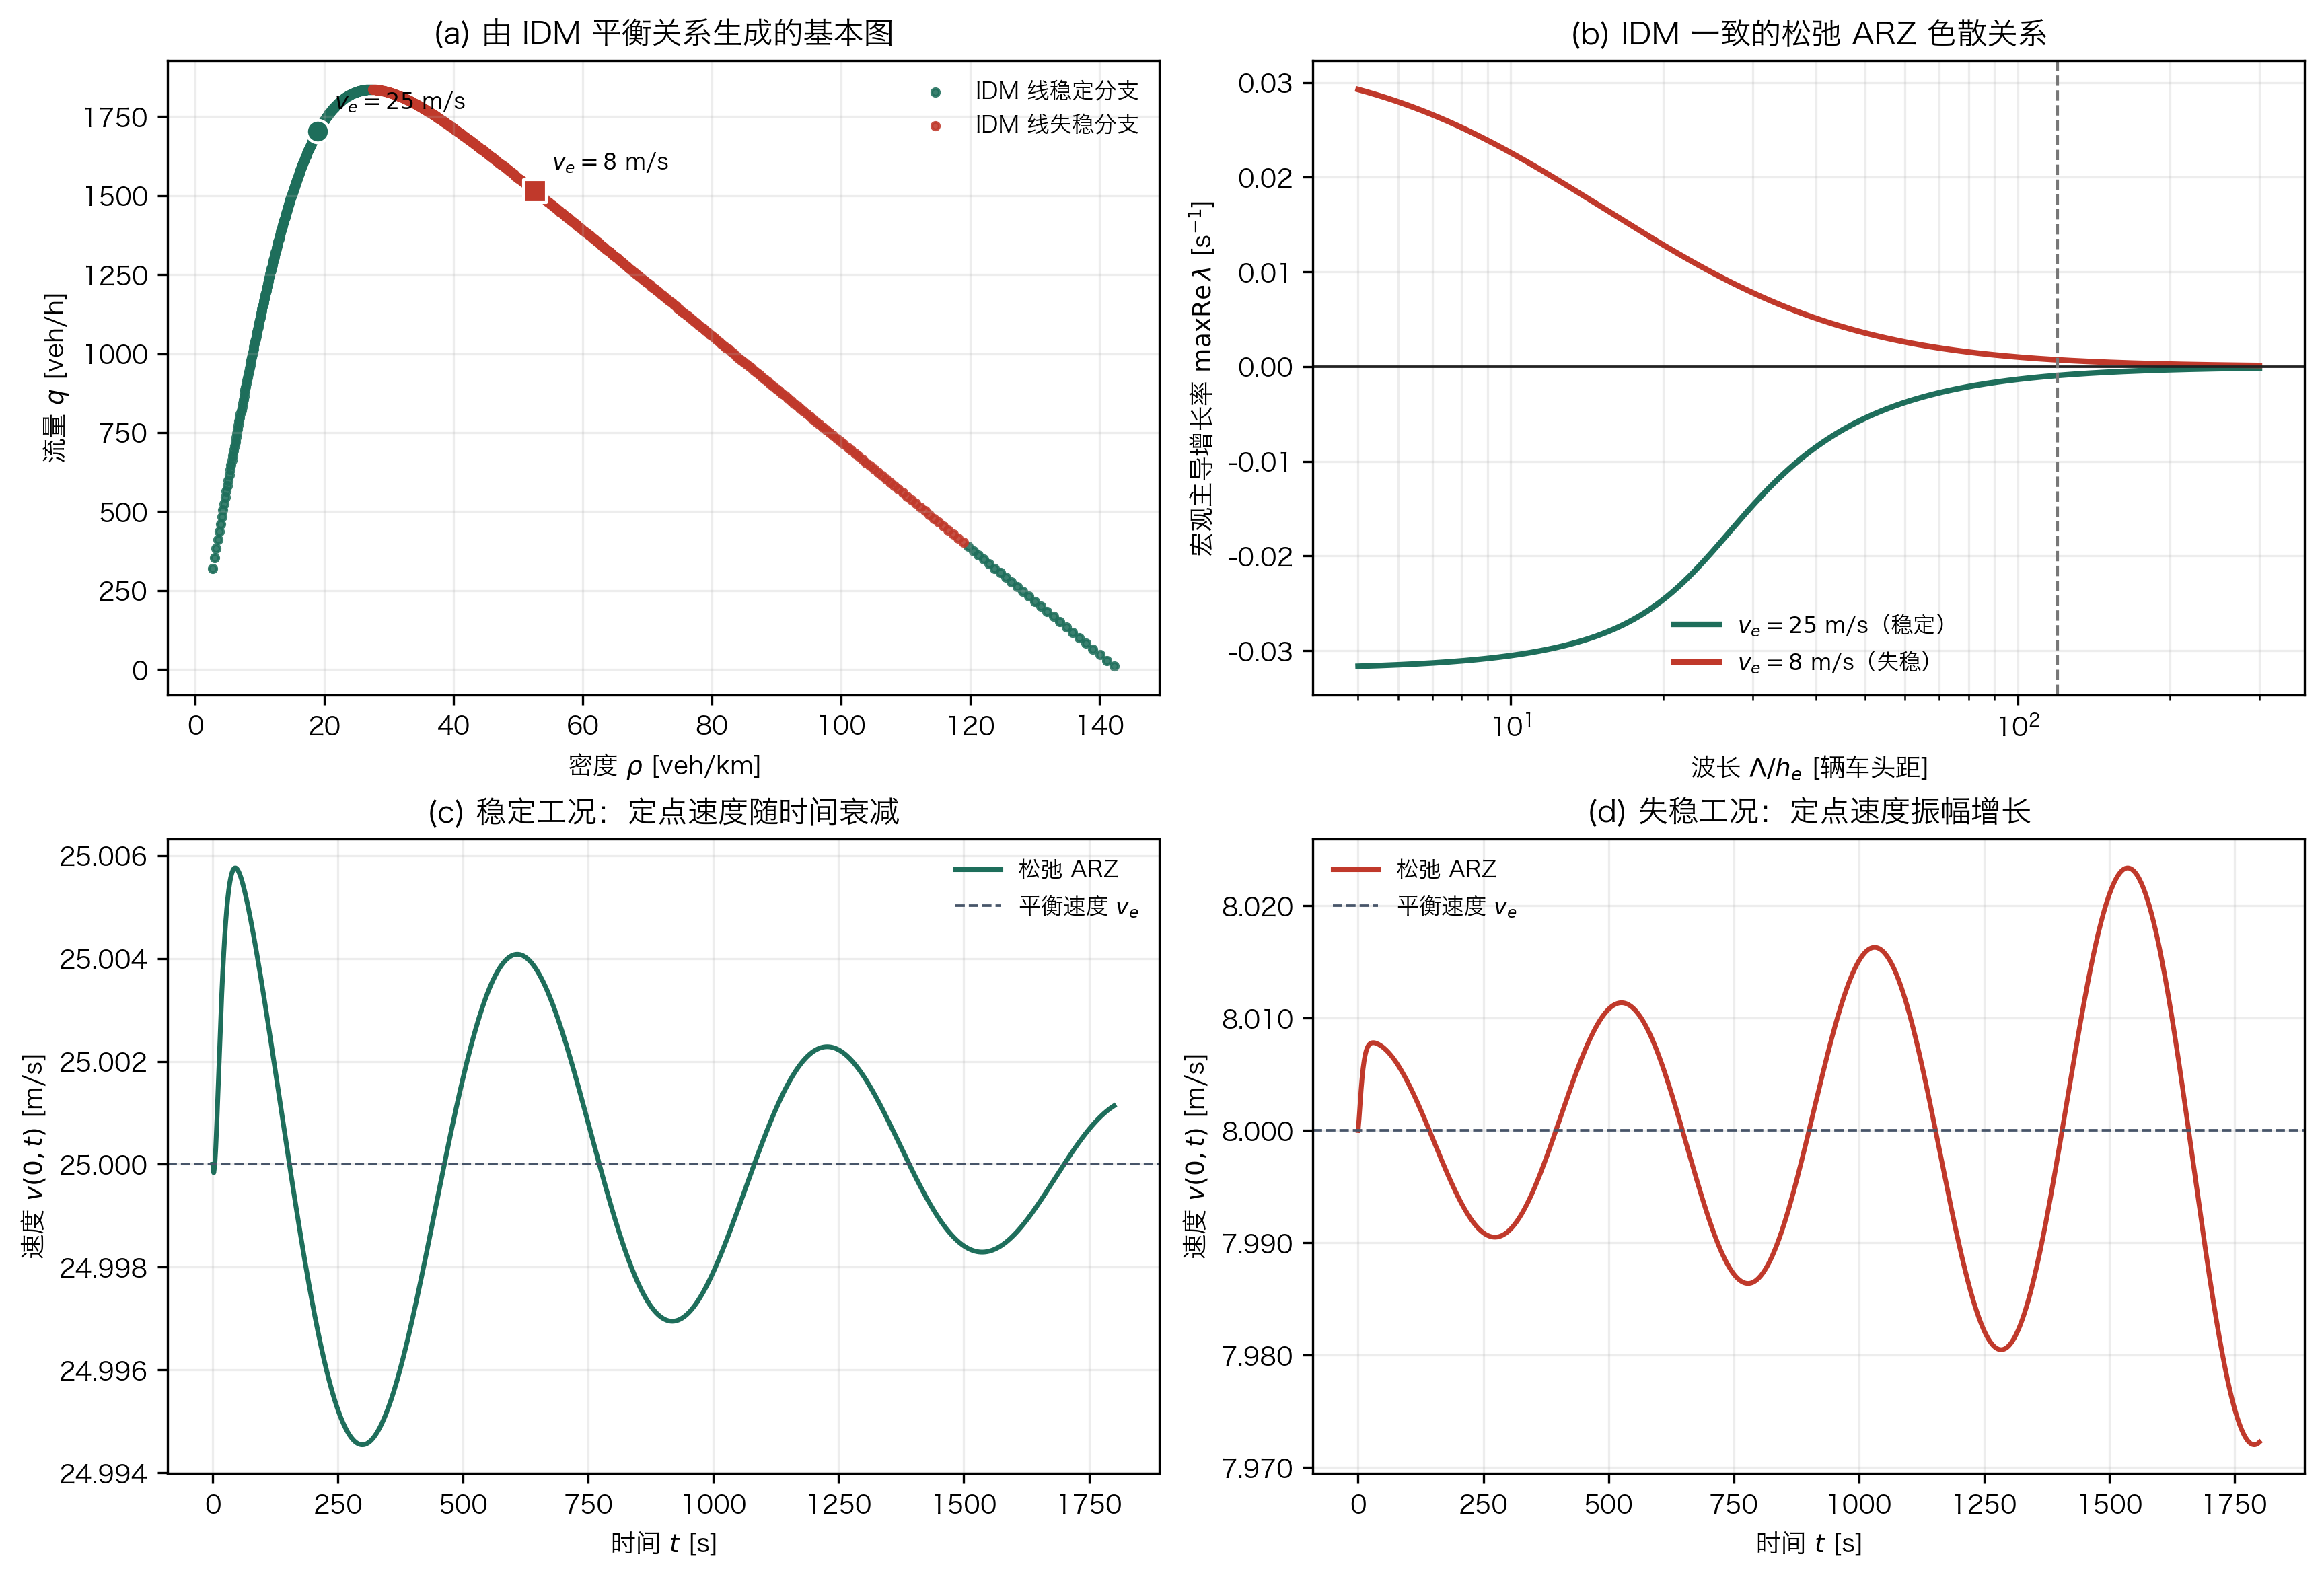
\includegraphics[width=\textwidth]{macroscopic_stability.png}
\caption{IDM 一致 ARZ 的宏观稳定性算例。}
\label{fig:macro-stability}
\figurenote{E13 对 IDM 一致 ARZ 宏观稳定性的分层验证。面板 (a) 先在 IDM 基本图上标出稳定与失稳工作点，确保宏观模型没有换用另一条经验流量--密度曲线；面板 (b) 再比较连续 ARZ 色散关系与 $N=120,m=1$ 的实际离散长波，交点给出应在时域出现的增长率和相速。面板 (c) 的稳定定点速度振幅逐周期缩小，与负实部对应；面板 (d) 的失稳定点振幅逐周期增大，与正实部对应，且周期与色散关系的虚部相符。由基本图一致到偏导闭合一致，再到频域和时域符号一致，排除了“只对齐平衡流量却动态相反”的情况。该图证明经 IDM 偏导标定的 ARZ 能在长波尺度复现微观模型的增长符号与主要时间尺度，但并不要求连续场复制每一辆离散车辆的局部纹理。}
\end{figure}

\begin{tcolorbox}[resultbox,title=\textbf{E13 的定量结论}]
在完全相同的 IDM 平衡曲线上，$v_e=25$ m/s 的 ARZ 长波在 1800 s 后只剩 $18.5\%$，而 $v_e=8$ m/s 的长波增长到 $360.6\%$。失稳工况的相速为负，表示波向上游传播；稳定工况相速为正，表示小扰动随交通向下游传播并消散。因此，\textbf{基本图决定平衡流量和运动学波速，动态闭合决定扰动是增长还是衰减；二者都必须与 IDM 一致。}
\end{tcolorbox}

\section{面对不同问题，应选哪一种宏观工具？}
\sectionstudy{theory}{面对不同问题，应选哪一种宏观工具？}{treiberkesting2011,daganzo1995,awrascle2000}

\begin{center}
\small
\captionof{table}{宏观交通问题与分析工具的对应。}
\label{tab:macro-tool-selection}
\begin{tabular}{p{3.0cm}p{4.1cm}p{6.8cm}}
\toprule
问题 & 推荐模型／工具 & 能回答什么，不能回答什么 \\
\midrule
排队、激波、拥堵前沿速度 & LWR／CTM & 用基本图和守恒准确计算波速、排队长度；理想 LWR 不提供内禀增长率。\\
平滑化与耗散 & 黏性 LWR & $D>0$ 给出 $-Dk^2$ 衰减；需区分物理扩散和数值扩散。\\
走停波的线性生成 & PW、ARZ 等二阶松弛模型 & 用色散关系与次特征条件求增长率、主导波长；必须检查双曲性与各向异性。\\
有限幅激波与相变 & 非线性守恒律、行波／分岔分析 & 研究激波、稀疏波、迟滞和相共存；不能只靠平衡点线性化。\\
入口、出口和固定瓶颈 & 开边界谱、对流／绝对稳定性 & 判断扰动是被带走还是占据固定位置；只检查周期边界的实 $k$ 谱不够。\\
模型与控制器标定 & 微观--宏观一致性检验 & 同时对齐基本图、松弛时间、波速和增长率；只拟合流量--密度曲线不足以保证动态稳定性正确。\\
\bottomrule
\end{tabular}
\end{center}
\tabletext{tab:macro-tool-selection}{排队、平滑化、走停波、有限幅激波、开边界和控制标定六类问题的推荐工具及能力边界。它说明稳定性问题必须先区分研究对象：LWR 的守恒激波、二阶模型的模态增长和开放边界的对流／绝对失稳不能用同一个判据替代。}

\begin{tcolorbox}[keybox,title=\textbf{本章与前文的关系}]
微观模型告诉我们\textbf{哪一种车辆响应、反馈拓扑或异质排列}导致扰动逐车放大；宏观模型告诉我们\textbf{密度／速度波以多快传播、在道路空间中如何形成激波或增长}。一阶 LWR 的运动学激波、二阶模型的线性失稳、微观车队的串不稳定是三个相关但不能互换的概念。把三者连起来，才可以从控制器参数一直解释到道路上的拥堵波图像。
\end{tcolorbox}

%==================================================================
\sectionwrapup{LWR 的无扩散小扰动是中性输运，PW 与 ARZ 则各有松弛根和水动力根；水动力根的 $k^2$ 项决定长波增长。开放道路还需用复波数钳夹判据区分对流与绝对失稳，不能仅凭环道实波数谱下结论。}

\chapter{宏观与微观的定量联系：IDM 一致的连续流极限}
\label{sec:micro-macro-bridge}
\chapterguide{怎样让宏观模型与 IDM 在同一工况下真正可比}{本章由车头距--密度关系和拉格朗日--欧拉坐标变换连接两种尺度，再用 IDM 基本图和动态偏导标定宏观闭合，使平衡流量、波速与长波增长率逐层一致。}

上一章分别介绍了微观跟驰模型和宏观连续流模型，但“二者相关”还不等于“二者数值一致”。如果宏观模型使用 Greenshields 基本图，而微观模型使用 IDM 平衡关系，即使两者都在讨论同一个速度，平衡密度、波速和容量点也并不相同；再任意选择宏观松弛时间和压力函数，稳定边界更没有理由一致。本章建立一条可计算的桥梁：\textbf{平衡层由 IDM 生成基本图，动态层由 IDM 长波系数标定宏观闭合}。PW 用来展示最简对称压力闭合，最终时空图则采用交通各向异性更合理的松弛 ARZ。

\section{第一层一致性：由 IDM 生成宏观基本图}
\sectionstudy{model}{第一层一致性：由 IDM 生成宏观基本图}{jin2003,helbing2001,treiberkesting2013}

对均匀 IDM，净间距是平衡速度的函数：
\begin{equation}
s_e(v)=\frac{s_0+vT}{\sqrt{1-(v/v_0)^\delta}}.
\label{eq:bridge-idm-gap}
\end{equation}
令车头间距 $h_e=s_e+\ell$。为什么密度是 $1/h_e$？取一段包含 $M$ 个连续车头距的道路，其长度约为 $Mh_e$、车辆数为 $M$，因此当平均尺度足够大时
\begin{equation}
\rho_e(v)=\lim_{M\to\infty}\frac{M}{Mh_e(v)}=\frac{1}{h_e(v)},
\qquad
q_e(v)=\rho_e(v)v.
\label{eq:bridge-idm-fundamental}
\end{equation}
式~\eqref{eq:bridge-idm-fundamental} 是参数形式的 IDM 基本图；不需要另行假设 Greenshields、Underwood 或三角形基本图。它保证微观和宏观在任一给定 $v_e$ 下具有相同的 $s_e$、$\rho_e$ 和 $q_e$。

沿平衡曲线对 $v=V(s)$ 求导，并利用 $\rho=1/(s+\ell)=1/h$。由于
\begin{equation}
\frac{\mathrm d\rho}{\mathrm ds}=-\frac{1}{(s+\ell)^2}=-\frac1{h^2},
\qquad
\frac{\mathrm ds}{\mathrm d\rho}=-h^2,
\end{equation}
链式法则给出
\begin{equation}
V_\rho
=\frac{\mathrm dV}{\mathrm ds}\frac{\mathrm ds}{\mathrm d\rho}
=-h^2V_s,
\qquad
q'(\rho)=V+\rho V_\rho=V-hV_s.
\label{eq:bridge-wave-speed}
\end{equation}
因此，只要宏观基本图来自同一个 IDM，LWR 的运动学波速 $q'(\rho)$ 就自动等于微观长波在道路坐标中的传播速度。基本图一致解决的是\textbf{相位速度}，但尚未解决增长率。

\section{第二层一致性：把微观长波系数变成宏观闭合}
\sectionstudy{theory}{第二层一致性：把微观长波系数变成宏观闭合}{jin2003,helbing2001,treiberkesting2013}

记基准跟驰模型在线性化后的偏导为 $f_s,f_v,f_{v_l}$，并定义
\begin{equation}
\mu=f_v+f_{v_l}<0.
\label{eq:bridge-mu}
\end{equation}
第~\ref{sec:appx}~章已经得到车辆编号坐标中的长波展开
\begin{equation}
\lambda_{\rm mic}(k)
=-\mathrm{i}c_1k-c_2k^2+O(k^3),
\qquad
c_1=-\frac{f_s}{\mu},
\qquad
c_2=\frac{c_1^2-\frac12f_s-f_{v_l}c_1}{\mu}.
\label{eq:bridge-micro-longwave}
\end{equation}
这里的 $n$ 是\textbf{拉格朗日坐标}：观察者跟着某个车辆编号移动；宏观模型的 $x$ 是\textbf{欧拉坐标}：观察者站在固定道路位置。二者的转换可以直接从均匀轨迹写出。由于本书的车辆编号向上游增加，平衡轨迹为
\begin{equation}
x_n^0(t)=V_et-nh_e,
\qquad
n=\frac{V_et-x}{h_e}.
\label{eq:bridge-label-position}
\end{equation}
若 $g(n,t)=G(x,t)$ 表示同一个缓慢变化的扰动，则链式法则给出
\begin{equation}
\left.\frac{\partial g}{\partial t}\right|_n
=\left.\frac{\partial G}{\partial t}\right|_x+V_eG_x,
\qquad
g_n=-h_eG_x,
\qquad
g_{nn}=h_e^2G_{xx}.
\label{eq:bridge-derivative-transform}
\end{equation}
车辆编号坐标中的长波方程与式~\eqref{eq:bridge-micro-longwave} 等价：
\begin{equation}
g_t+c_1g_n=c_2g_{nn}.
\label{eq:bridge-lagrangian-pde}
\end{equation}
将式~\eqref{eq:bridge-derivative-transform} 逐项代入：
\begin{align}
G_t+V_eG_x+c_1(-h_eG_x)&=c_2h_e^2G_{xx},\\
G_t+\underbrace{(V_e-h_ec_1)}_{q'(\rho_e)}G_x
&=\underbrace{c_2h_e^2}_{D_{\rm IDM}}G_{xx}.
\label{eq:bridge-eulerian-pde}
\end{align}
对欧拉 Fourier 模态 $G\propto e^{\lambda t+\mathrm{i}Kx}$，便得到
\begin{equation}
\lambda_{\rm mic}^{(x)}(K)
=-\mathrm{i}K\underbrace{(V_e-h_ec_1)}_{q'(\rho_e)}
-\underbrace{c_2h_e^2}_{D_{\rm IDM}}K^2
+O(K^3h_e^3),
\qquad K=\frac{k}{h_e}.
\label{eq:bridge-eulerian-longwave}
\end{equation}
这一步也可用相位检查：在 $e^{\lambda t+\mathrm{i}kn}$ 中代入 $n=(V_et-x)/h_e$，会同时产生车辆平移项 $V_e$ 和编号传播项 $-h_ec_1$；两者相减才是道路坐标中的波速。车辆本身可以向下游行驶，而当 $V_e-h_ec_1<0$ 时，拥堵波仍向上游传播。

其中
\begin{equation}
D_{\rm IDM}=c_2h_e^2
\label{eq:bridge-idm-diffusion}
\end{equation}
就是微观 IDM 在道路尺度上的等效扩散：$c_2>0$ 时 $D_{\rm IDM}>0$，扰动衰减；$c_2<0$ 时为负扩散，长波增长。这里并非凭空“把车辆编号换成米”：一阶导数带来一个 $h_e$，二阶导数带来 $h_e^2$，所以 $D_{\rm IDM}$ 的单位正好是 m$^2$/s。

\section{第三层一致性：分别标定 PW 与 ARZ 动态闭合}
\sectionstudy{theory}{第三层一致性：分别标定 PW 与 ARZ 动态闭合}{payne1971,daganzo1995,jin2003}

先匹配 $k=0$ 的快速恢复根。微观快速根为 $\mu=f_v+f_{v_l}<0$，PW 和 ARZ 的快速根都是 $-1/\tau$，因此
\begin{equation}
\boxed{\tau=-\frac1\mu.}
\label{eq:bridge-tau-calibration}
\end{equation}

PW 型宏观模型的长波根由式~\eqref{eq:pw-hydro-root} 给出。要求 $D_{\rm eff}=D_{\rm IDM}$，得到
\begin{equation}
\boxed{
c_0^2=(\rho_eV_\rho)^2+\frac{D_{\rm IDM}}{\tau}
}
\label{eq:bridge-pw-calibration}
\end{equation}
于是 PW 同时匹配：
\begin{enumerate}[leftmargin=1.5em,itemsep=3pt]
\item $k=0$ 的快速速度恢复根：$-1/\tau=\mu$；
\item 一阶相位项：$V+\rho V_\rho=V-hc_1$；
\item 二阶增长／衰减项：$D_{\rm eff}=D_{\rm IDM}=c_2h^2$。
\end{enumerate}

对 ARZ，记
\begin{equation}
A=\rho_eV_\rho=-h_ec_1<0,
\qquad
B=\rho_ep'(\rho_e)>0.
\end{equation}
由式~\eqref{eq:arz-effective-diffusion}，$D_{\rm ARZ}=-\tau A(A+B)$。令它等于 $D_{\rm IDM}$，可直接解出所需的局部压力斜率：
\begin{equation}
\boxed{
B=-\frac{D_{\rm IDM}}{\tau A}-A,
\qquad
p'(\rho_e)=\frac{B}{\rho_e}.
}
\label{eq:bridge-arz-calibration}
\end{equation}
稳定工况 $D_{\rm IDM}>0$ 时，式~\eqref{eq:bridge-arz-calibration} 给出 $B>-A$，所以 LWR 波速 $V+A$ 位于 ARZ 的 $[V-B,V]$ 内；失稳工况 $D_{\rm IDM}<0$ 时，$B<-A$，次特征条件恰好被违反。ARZ 因而不仅复制增长率符号，也复制其“是否满足次特征条件”的物理原因。

\begin{tcolorbox}[notebox,title=\textbf{为什么只替换基本图还不够？}]
基本图只固定 $V(\rho)$ 和 $q'(\rho)$，并不包含驾驶者多快恢复、相对速度反馈有多强等动态信息。两个模型可以拥有完全相同的流量--密度曲线，却有一个稳定、另一个失稳。式~\eqref{eq:bridge-tau-calibration}--\eqref{eq:bridge-arz-calibration} 把 IDM 的动态偏导也带入宏观模型，才使稳定符号和长波增长率趋于一致。本书保留 PW 参数用于解析交叉检查，但 E13/E14 的主图采用 ARZ，因为它同时满足 IDM 长波匹配与交通各向异性。
\end{tcolorbox}

\section{两个基准工况的闭合参数}
\sectionstudy{model}{两个基准工况的闭合参数}{jin2003,helbing2001,treiberkesting2013}

代入第~\ref{sec:num}~章的基准 IDM 参数，得到：
\begin{center}
\captionof{table}{IDM 一致的 PW/ARZ 闭合参数。}
\label{tab:bridge-closure-parameters}
\resizebox{\textwidth}{!}{%
\begin{tabular}{lrrrrrr}
\toprule
工况 & $v_e$ & $\rho_e$ & $\tau$ & $D_{\rm IDM}$ & $c_0$（PW） & $B=\rho p'$（ARZ） \\
& [m/s] & [veh/km] & [s] & [m$^2$/s] & [m/s] & [m/s] \\
\midrule
稳定 & 25 & 18.933 & 9.742 & $+951.43$ & 17.700 & 21.335 \\
失稳 & 8 & 52.567 & 4.646 & $-97.46$ & 11.699 & 10.893 \\
\bottomrule
\end{tabular}
}
\end{center}
\tabletext{tab:bridge-closure-parameters}{稳定和失稳工作点由 IDM 动态偏导唯一确定的松弛时间、等效扩散、PW 声速和 ARZ 压力斜率。稳定行满足次特征条件并给出正扩散，失稳行同时出现次特征条件违反和负扩散，说明这里的宏微观一致不是只对齐基本图。}
稳定工况有 $-A=14.684$ m/s，而 $B=21.335>-A$，ARZ 次特征条件成立；失稳工况有 $-A=12.563$ m/s，而 $B=10.893<-A$，次特征条件违反。表中的 $c_0$ 与 $B$ 都不是人为调到“想要的结果”，而是分别由式~\eqref{eq:bridge-pw-calibration} 与式~\eqref{eq:bridge-arz-calibration} 对每个平衡点确定的局部闭合值。

\section{E14：相同 IDM 条件下的微观--宏观时空图}
\sectionstudy{experiment}{E14：相同 IDM 条件下的微观--宏观时空图}{jin2003,helbing2001,treiberkesting2013}
\label{sub:micro-macro-experiment}

两种模型使用完全相同的 $v_e$、$\rho_e$、环道长度和初始扰动：
\begin{itemize}[leftmargin=1.4em,itemsep=3pt]
\item $N=120$，取最长的非零环道模态 $m=1$，故 $\Lambda=L=N(s_e+\ell)$；
\item 初始速度扰动为 $0.05\sin(2\pi n/N)$ m/s，初始间距均匀；
\item 仿真时间 1800 s；微观侧积分完整非线性 IDM，RK4 步长 $0.05$ s；
\item 宏观侧用谱方法精确推进线性化松弛 ARZ，并按式~\eqref{eq:bridge-tau-calibration}、\eqref{eq:bridge-arz-calibration} 使用 IDM 一致闭合；
\item 图~\ref{fig:micro-macro-idm} 横轴为时间，纵轴为归一化道路位置 $x/L$，颜色为速度扰动 $v-v_e$。
\end{itemize}
之所以使用 $x/L$ 而不是绝对公里数，是因为两个平衡密度不同：稳定工况环长为 6.338 km，失稳工况为 2.283 km。归一化位置使两行都显示完整一圈，同时不改变波的斜率方向。

\begin{figure}[!t]
\centering
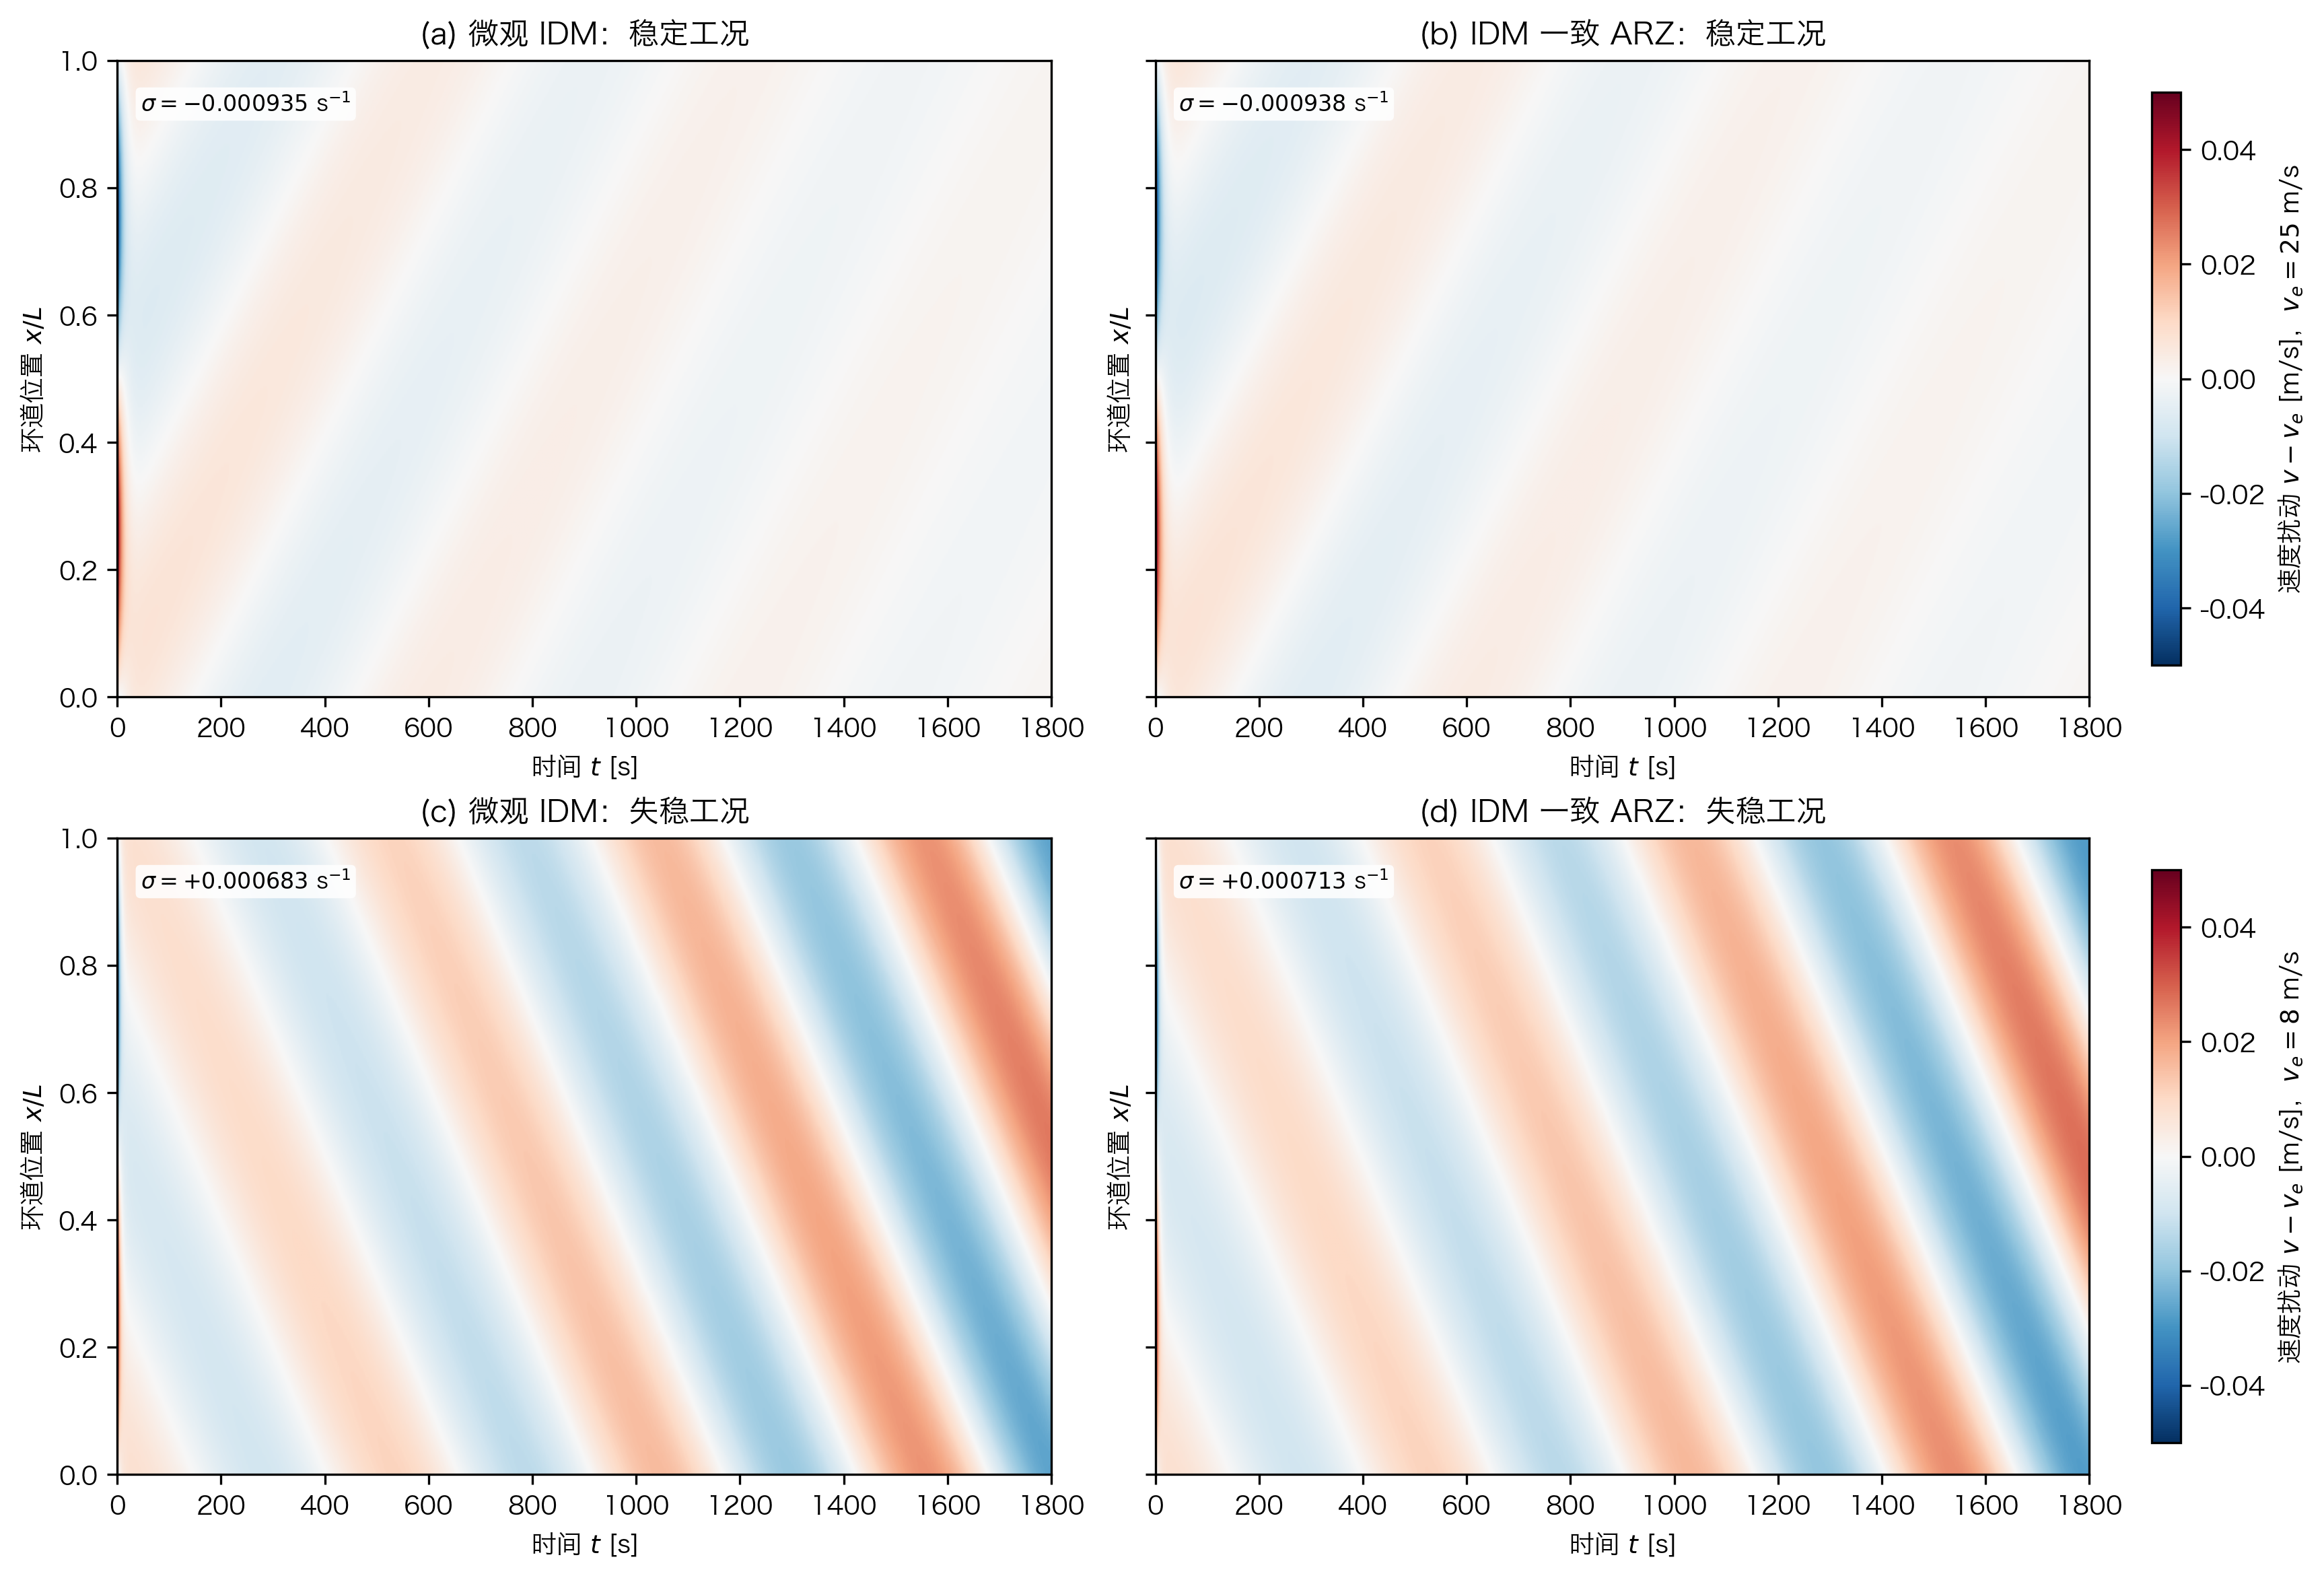
\includegraphics[width=\textwidth]{micro_macro_idm_comparison.png}
\caption{IDM--ARZ 的宏微观速度时空图对照。}
\label{fig:micro-macro-idm}
\figurenote{E14 在固定道路坐标中直接比较微观 IDM 与宏观 ARZ 的速度时空场。两列使用同一 IDM 基本图、同一 $v_e$、密度、环长和初始 $m=1$ 长波；每一行共用颜色范围，横轴为时间，纵轴为 $x/L$，所以色带斜率和深浅可以直接比较。稳定行 $v_e=25$ m/s 中，两种模型的正负扰动带均随时间变淡，传播斜率接近，证明它们对衰减率和相速给出一致预测；失稳行 $v_e=8$ m/s 中，色带向较小 $x$ 倾斜并逐渐增强，证明两种尺度都预测上游传播的增长波。微观图保留一条条车辆轨迹和更细纹理，宏观图则是平滑连续场，这些局部差异来自尺度表示而非稳定结论冲突。该图证明只有同时匹配 IDM 基本图、松弛时间和压力斜率，宏微观模型才会在相同条件下给出相似的道路时空演化。}
\end{figure}

\section{增长率、波速和图像相似度的定量比较}
\sectionstudy{theory}{增长率、波速和图像相似度的定量比较}{jin2003,helbing2001,treiberkesting2013}

\begin{center}
\small
\captionof{table}{IDM 与 IDM 一致 ARZ 的动态误差。}
\label{tab:micro-macro-dynamic-errors}
\begin{tabular}{lrrrrr}
\toprule
工况 & 模型 & $\operatorname{Re}\lambda$ [s$^{-1}$] & 相速 [m/s] & 增长率误差 & 波速误差 \\
\midrule
稳定 & 微观 IDM & $-0.0009355$ & $+10.293$ & -- & -- \\
稳定 & IDM 一致 ARZ & $-0.0009377$ & $+10.241$ & $0.24\%$ & $0.51\%$ \\
\midrule
失稳 & 微观 IDM & $+0.0006827$ & $-4.469$ & -- & -- \\
失稳 & IDM 一致 ARZ & $+0.0007126$ & $-4.516$ & $4.37\%$ & $1.05\%$ \\
\bottomrule
\end{tabular}
\end{center}
\tabletext{tab:micro-macro-dynamic-errors}{微观 IDM 与连续 ARZ 对同一长波的增长率和相速预测。两种尺度在稳定工况的误差均小于 $1\%$，在失稳工况也保持相同符号和传播方向；残余差异来自离散车辆与连续场以及有限波数高阶项。}

为避免仅凭肉眼说“很像”，把每个时刻的速度扰动场去均值并除以其空间标准差，再计算 0--1500 s 内微观与宏观场的平均相关系数：
\begin{equation}
\mathcal S
=\left\langle
\frac{u_{\rm mic}}{\sigma_{\rm mic}}
\frac{u_{\rm mac}}{\sigma_{\rm mac}}
\right\rangle_{x,t}.
\label{eq:bridge-similarity}
\end{equation}
稳定工况得到 $\mathcal S=0.9977$，失稳工况得到 $\mathcal S=0.9913$。这说明两者不仅稳定符号相同，红蓝色带的传播方向、倾斜角和相位位置也高度一致。1800 s 后，微观／ARZ 的理论幅值比分别为：
\begin{equation}
\begin{array}{c|cc}
&\text{微观 IDM}&\text{IDM 一致 ARZ}\\ \hline
v_e=25\ {\rm m/s}&0.186&0.185\\
v_e=8\ {\rm m/s}&3.417&3.606
\end{array}
\label{eq:bridge-amplitude-ratios}
\end{equation}

\begin{tcolorbox}[resultbox,title=\textbf{E14 的核心结论}]
\begin{itemize}[leftmargin=1.3em,itemsep=3pt]
\item 用 IDM 基本图替代 Greenshields 后，微观和宏观首先在密度、流量及运动学波速上保持一致。
\item 再用 IDM 偏导标定 $\tau$、$p'(\rho_e)$ 和 $D_{\rm ARZ}$，两者才在稳定符号、增长率和传播速度上趋于一致。
\item $v_e=25$ m/s 时两幅色带随时间变淡；$v_e=8$ m/s 时两幅色带均向上游倾斜并加深。稳定／失稳不再依赖人为挑选不同宏观参数。
\end{itemize}
\end{tcolorbox}

\section{这种一致性到哪里为止？}
\sectionstudy{synthesis}{这种一致性到哪里为止？}{jin2003,helbing2001,treiberkesting2013}

本章验证的是\textbf{小扰动、长波、均匀单车道}极限。宏观模型只匹配到 $O(K^2)$；有限波长处的 $O(K^3)$ 色散、离散车辆造成的高波数截断，以及停止--启动后的非线性饱和仍由完整 IDM 决定。因此：
\begin{itemize}[leftmargin=1.4em,itemsep=3pt]
\item 当 $m/N\to0$ 时，增长率和波速误差应继续减小；
\item 当扰动已经发展为停车波时，线性宏观闭合不能替代完整微观仿真；
\item 异质车辆、换道、通信拓扑和反应延迟需要额外的宏观状态或非局部闭合，不能只靠一条 IDM 基本图保留。
\end{itemize}
这也说明宏观模型不是微观模型的“另一张画法”，而是经过空间平均和尺度截断后的近似；一致性必须明确说明匹配了哪些阶次和哪些观测量。

%==================================================================
\sectionwrapup{IDM 基本图使宏微观平衡密度、流量和运动学波速一致；拉格朗日到欧拉坐标变换进一步把车辆编号波数、道路波长和长波扩散系数对应起来。只有再由 IDM 动态偏导标定 $\tau$ 与 $p'(\rho)$，宏观与微观的增长率才可能定量吻合。}

\chapter{真实轨迹中的稳定性证据：NGSIM}
\label{sec:ngsim}
\chapterguide{怎样把真实轨迹真正用于稳定性建模与决策}{本章先用 D01 从位置--时间轨迹、连续八车队和 78 个自然片段中提取传播证据，再用 D02 完整走过“稳定性车队标定--留出模拟验证--稳定性优化与评估”三大块，并明确哪些结论来自数据、哪些来自模型反事实。}

前面的稳定性结论建立在明确模型和平衡态上。真实道路则同时包含换道、匝道、驾驶差异、测量误差和不断变化的边界输入，因此不能把一段红蓝相间的实测时空图直接称为“线性失稳”。真实数据分析更适合回答四个逐层加深的问题：
\begin{enumerate}[leftmargin=1.6em,itemsep=3pt]
\item 是否能从同车道连续前后车中识别出相干的速度扰动？
\item 跟车的波动幅值相对前车是增大还是减小，响应滞后多长？
\item 相比只拟合一辆跟车，加入整列车传播信息后，模型能否在留出时段更好地复现交通流？
\item 能否把标定模型的稳定性谱变成控制参数，再用独立仿真和留出数据分别评价？
\end{enumerate}
D01 回答前两项；D02 回答后两项。它们共同形成一个完整应用示范，但仍不宣称仅凭一个三分钟样本完成 IDM 的普适标定或控制器道路验证。

\section{数据源、观测区间与字段}
\sectionstudy{data}{数据源、观测区间与字段}{ngsim2016,thiemann2008,krajewski2018}

NGSIM 由美国联邦公路管理局组织采集，US--101 数据使用同步视频重建车辆轨迹，官方开放数据按约 $0.1$ s 给出一条记录，并推荐用数据集 DOI 引用\cite{ngsim2016}。D01 从官方数据接口读取 US--101 南向车道 2 的一个 $179.5$ s 片段，查询区间为
\[
1118846979700\le \texttt{global\_time}\le1118847159700.
\]
返回 39187 行、119 辆车；这一片段的 \texttt{v\_class} 均为 2，即乘用车辆。原始纵向位置、速度、加速度和空间车头距采用英尺制，进入分析后统一乘 $0.3048$ 转为 SI 单位。

\begin{center}
\small
\captionof{table}{D01 使用的 NGSIM 字段与预处理。}
\label{tab:ngsim-fields}
\begin{tabular}{p{3.2cm}p{4.8cm}p{5.4cm}}
\toprule
\textbf{字段} & \textbf{本章用途} & \textbf{处理} \\
\midrule
\texttt{vehicle\_id}, \texttt{global\_time} & 唯一轨迹与共同时间轴 & 检查相邻帧是否相差 100 ms \\
\texttt{local\_y}, \texttt{v\_vel} & 位置--时间速度着色轨迹 & ft、ft/s 分别转为 m、m/s \\
\texttt{preceding}, \texttt{lane\_id} & 重建同车道前后车链 & 前车编号不变才视为同一片段 \\
\texttt{space\_headway}, \texttt{time\_headway} & 间距和时距描述 & 去除前车编号为 0 的边界记录 \\
\texttt{v\_acc} & 加速度诊断 & 只作辅助；不直接用原始差分量标定模型 \\
\bottomrule
\end{tabular}
\end{center}
\tabletext{tab:ngsim-fields}{从官方轨迹记录中用于重建车队、生成位置--时间图并计算传播增益的字段。表中同时列出单位换算和连续性检查，说明 D01 的稳定性证据并非直接使用噪声较大的原始加速度。}

\begin{tcolorbox}[notebox,title=\textbf{为什么本章不直接拟合原始加速度}]
位置重建的微小误差在两次时间差分后会被显著放大，换道附近的前车切换又会造成不连续。D01 因此把速度作为主观测量，并对平滑窗口做显式记录。后续若标定 IDM，加速度残差只能与轨迹、间距、传播增益和留出集误差一起使用，不能作为唯一目标。
\end{tcolorbox}

\section{D01 的可复现处理流程}
\sectionstudy{data}{D01 的可复现处理流程}{ngsim2016,thiemann2008,krajewski2018}

数据管线按下列固定顺序执行：
\begin{enumerate}[leftmargin=1.6em,itemsep=3pt]
\item 从官方 API 读取指定地点、车道、时间和字段，保存查询条件与访问日期；
\item 按 \texttt{global\_time, vehicle\_id} 排序，校验字段并完成单位转换；
\item 在约第 100 s 的共同快照中寻找最长 \texttt{preceding} 链，取其中连续观测不少于 20 s 的 8 辆车；
\item 对所有前车编号不变且连续不少于 201 帧的跟驰片段，使用 21 帧三阶 Savitzky--Golay 滤波\cite{savitzky1964}；
\item 对每条速度曲线去除线性趋势，排除前车标准差小于 $0.25$ m/s 的近常数片段；
\item 计算逐车幅值增益、最大相关滞后，并用固定随机种子自助抽样 20000 次给出不确定区间。
\end{enumerate}

若平滑并去趋势后的前车、跟车速度分别为 $\widetilde v_l(t)$ 与 $\widetilde v_f(t)$，本章的经验增益定义为
\begin{equation}
\Gamma_{f\leftarrow l}
=\frac{\operatorname{std}(\widetilde v_f)}
       {\operatorname{std}(\widetilde v_l)},
\qquad
\tau^*=\arg\max_{0\le\tau\le5\,\mathrm s}
\operatorname{corr}\!\left[\widetilde v_l(t),\widetilde v_f(t+\tau)\right].
\label{eq:ngsim-gain}
\end{equation}
$\Gamma>1$ 表示这一个自然片段中跟车波动较大，$\Gamma<1$ 表示较小。它与稳态正弦实验的 $|G(\mathrm i\omega)|$ 有联系，却不是同一个量：式~\eqref{eq:ngsim-gain} 混合了片段中存在的多个频率，并且未控制所有外部输入。

\begin{tcolorbox}[experimentbox,title=\textbf{D01 伪代码与实际输出一一对应}]
\begin{verbatim}
download official slice -> validate schema -> convert ft to m
for each continuous leader-follower episode >= 20 s:
    smooth leader and follower speed with the declared window
    remove each linear trend
    if std(leader) >= 0.25 m/s:
        gain = std(follower) / std(leader)
        lag  = argmax cross_correlation over 0 ... 5 s
bootstrap the episode table -> confidence intervals
save derived CSV + JSON metrics + four-panel figure
\end{verbatim}
\end{tcolorbox}

\section{连续八车队：扰动不是整齐的单一正弦波}
\sectionstudy{theory}{连续八车队：扰动不是整齐的单一正弦波}{ngsim2016,thiemann2008,krajewski2018}

自动选出的链按领车到上游跟车依次为
\[
395\rightarrow399\rightarrow405\rightarrow411\rightarrow418\rightarrow426\rightarrow431\rightarrow440,
\]
共同观测 20.0 s。图~\ref{fig:ngsim-d01}(b) 显示不同车辆的速度峰谷存在明显滞后；图~\ref{fig:ngsim-d01}(c) 的去趋势标准差并不逐车单调变化，而是在中间车辆处衰减、到上游车辆 431 与 440 又增大。这正是真实数据与单一 Fourier 模态的区别：多个扰动、异质参数和边界输入同时存在，不能只用末车／首车两个数字概括整个传播过程。

\section{78 个自然跟驰片段的统计结果}
\sectionstudy{data}{78 个自然跟驰片段的统计结果}{ngsim2016,thiemann2008,krajewski2018}

筛选后得到 78 个连续片段。样本的中位时间车头距为 1.77 s，四分位区间为 1.44--2.18 s；中位响应滞后为 1.85 s，中位最大相关系数为 0.794。经验增益的结果为
\begin{equation}
\operatorname{median}(\Gamma)=1.033,\qquad
\operatorname{IQR}(\Gamma)=[0.892,1.189],\qquad
\Pr_{\rm sample}(\Gamma>1)=55.1\%.
\label{eq:ngsim-results}
\end{equation}
但是，片段级自助抽样给出的中位数 95\% 区间为 $[0.954,1.077]$，放大片段比例的 95\% 区间为 $[44.9\%,65.4\%]$；两者均跨过中性参照值。因此正确结论不是“US--101 已被证明线不稳定”，而是：\textbf{该片段同时存在放大与衰减事件，中位经验增益接近 1，当前样本不足以在总体层面排除中性传播。}

\begin{figure}[htbp]
\centering
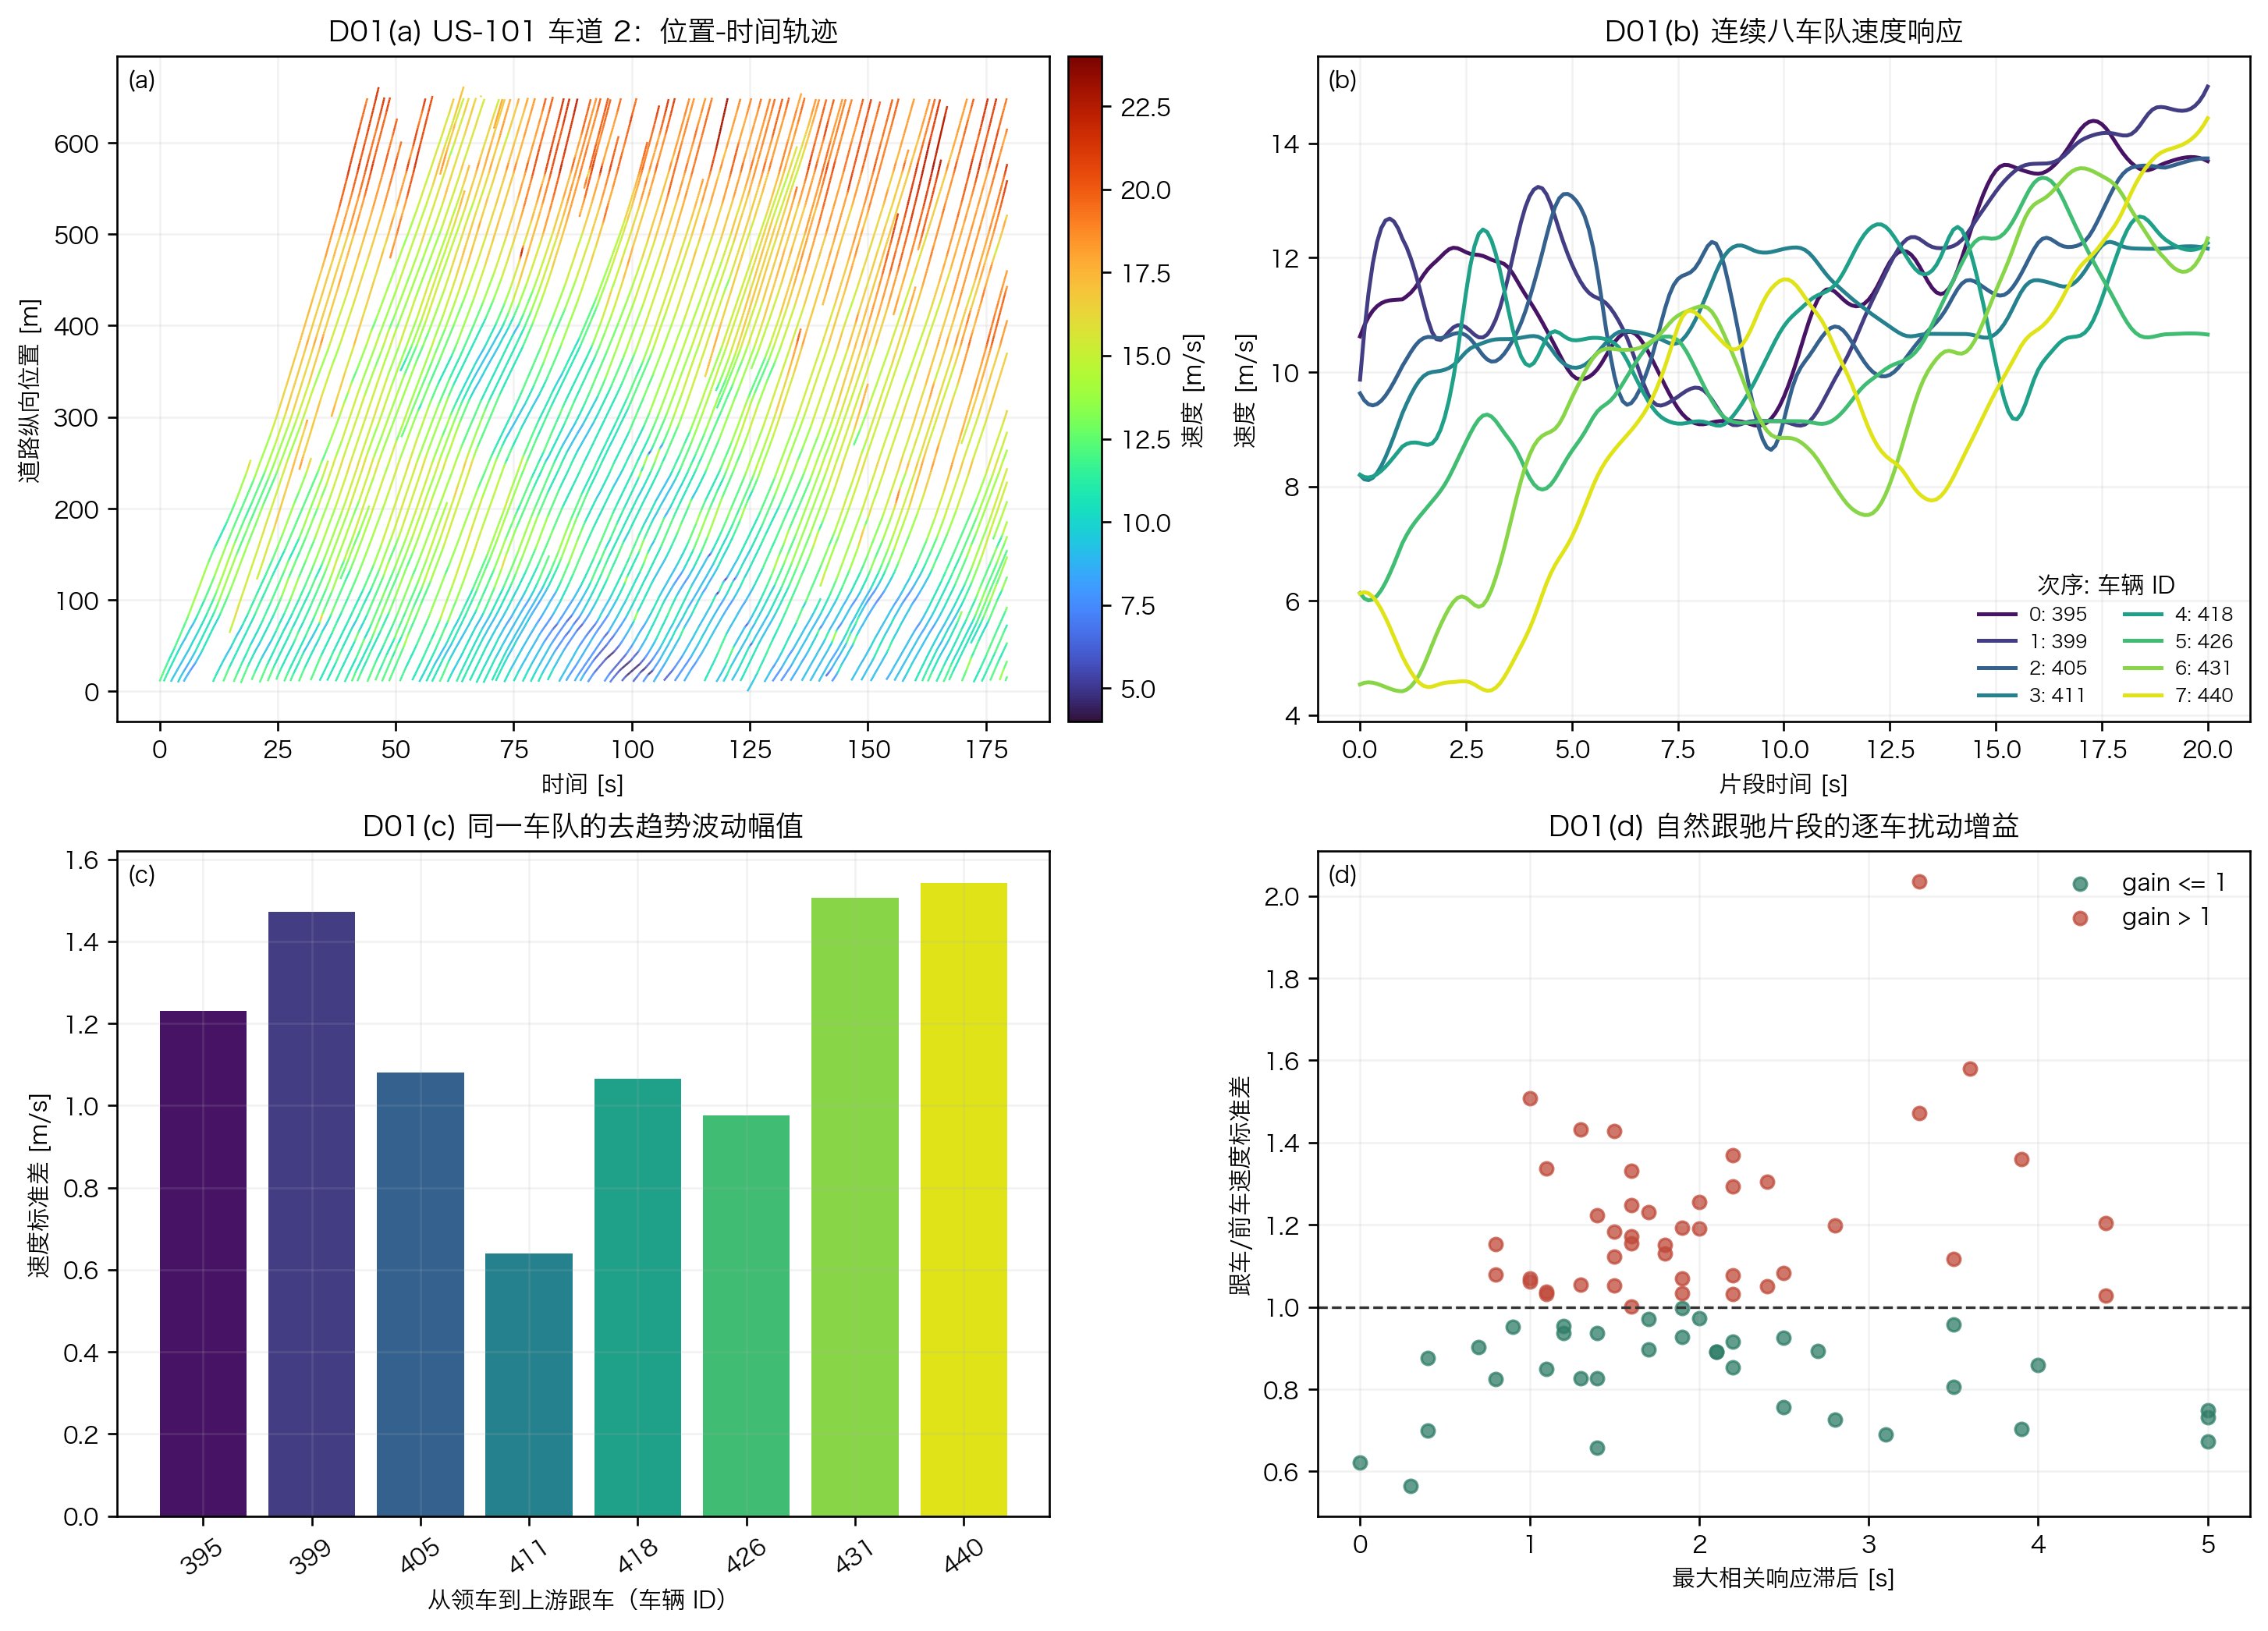
\includegraphics[width=\textwidth]{ngsim_us101_d01.png}
\caption{NGSIM US--101 真实轨迹的稳定性诊断。}
\label{fig:ngsim-d01}
\figurenote{D01 从 NGSIM US--101 原始轨迹到经验稳定性证据的完整处理链。面板 (a) 在真实位置--时间图上显示车道 2 的车辆轨迹和速度颜色，先确认所选时段确有可传播的速度波；面板 (b) 展开自动识别的连续八车队，峰谷沿车序出现时间滞后，说明车辆间存在因果传播而非同时外部输入。面板 (c) 比较去趋势后的逐车速度标准差，可见扰动并非单调增大或减小，而是在异质车辆之间局部衰减后再次放大；这解释了为什么只比较首车和末车会遗漏中途结构。面板 (d) 汇总 78 个自然跟驰片段的经验增益与滞后，红点只表示该片段 $\Gamma>1$，中位数接近 1 且不确定区间跨过中性值。该图证明真实交通同时包含放大与衰减事件，支持把稳定性作为统计标定目标，但不足以单凭一个三分钟样本宣称整条 US--101 全局线不稳定；红点也不是碰撞风险标签。}
\end{figure}

\section{D02 总体设计：从真实车队到可评价的稳定性应用}
\sectionstudy{data}{D02 总体设计：从真实车队到可评价的稳定性应用}{kesting2008,ossen2009,punzo2012}
\label{sub:ngsim-d02}

D02 使用 D01 自动选出的八车队
\[
395\rightarrow399\rightarrow405\rightarrow411\rightarrow418
\rightarrow426\rightarrow431\rightarrow440
\]
完成三块工作。$0$--$12$ s 用于标定，$12$--$20$ s 完全留出；所有速度和空间车头距
先按 D01 的同一 21 帧三阶滤波处理。把空间车头距减去统一车长 $4.8$ m 得到净间距。
为减少这个短片段中的不可辨识参数，固定 $v_0=33.3$ m/s、$\delta=4$ 和车长，
只估计 $\theta=(T,s_0,a,b)$。

\begin{enumerate}[leftmargin=1.6em,itemsep=3pt]
\item \textbf{稳定性标定：}比较“只拟合第一辆跟车 399”和“同时拟合七辆跟车及逐车扰动幅值”；
\item \textbf{模拟验证：}冻结参数，从留出时刻的实测状态重新起步，只把领车 395 的留出速度作为外部输入，递推模拟其余七辆车；
\item \textbf{优化与评估：}用标定模型的环道谱选择最小前车加速度前馈增益，再分别检查模型环道和真实留出片段。
\end{enumerate}
这个拆分很重要：标定、验证和优化使用不同的信息角色，不能在看过留出结果后再回头调整参数。

\subsection{第一块：为什么稳定性标定不等于多加一个 RMSE}

传统单车目标只使用车辆 399：
\begin{equation}
J_{\rm one}(\theta)
=\frac{{\rm RMSE}(v_{399}^{\rm sim},v_{399}^{\rm obs})}{1\ {\rm m/s}}
+\frac{{\rm RMSE}(s_{399}^{\rm sim},s_{399}^{\rm obs})}{5\ {\rm m}}.
\label{eq:ngsim-single-objective}
\end{equation}
稳定性车队目标则同时积分七辆跟车。设
$A_j={\rm std}\{\operatorname{detrend}[v_j(t)]\}$ 为训练段的逐车速度幅值，定义
\begin{equation}
J_{\rm platoon}(\theta)
=\frac{{\rm RMSE}(\bm v^{\rm sim},\bm v^{\rm obs})}{1\ {\rm m/s}}
+\frac{{\rm RMSE}(\bm s^{\rm sim},\bm s^{\rm obs})}{5\ {\rm m}}
+1.25\,{\rm RMSE}\!\left(\log\bm A^{\rm sim},\log\bm A^{\rm obs}\right).
\label{eq:ngsim-platoon-objective}
\end{equation}
第三项不是简单“多用几辆车”：它要求模型保留扰动沿车序的空间形状，使一个局部轨迹拟合很好、
但把上游波动放大得完全错误的参数受到惩罚。两种目标均用相同参数边界和随机种子求解。

\begin{center}
\small
\captionof{table}{D02 两种目标标定得到的 IDM 参数。}
\label{tab:d02-calibrated-parameters}
\begin{tabular}{p{3.7cm}rrrr}
\toprule
\textbf{标定方法} & $T$ [s] & $s_0$ [m] & $a$ [m/s$^2$] & $b$ [m/s$^2$]\\
\midrule
单车 399 & 0.4458 & 6.000 & 2.257 & 4.500\\
稳定性车队 & 0.9474 & 6.000 & 1.550 & 0.500\\
\bottomrule
\end{tabular}
\end{center}
\tabletext{tab:d02-calibrated-parameters}{单车目标与稳定性车队目标得到的两组 IDM 参数。两者差异很大且均有参数触及边界，说明短时单车轨迹不能唯一识别车流层的扰动传播性质，必须把参数结果与训练和留出误差共同解释。}
若把两组参数都拿去重放\textbf{整个训练车队}，结果为
\begin{center}
\small
\captionof{table}{D02 训练车队的重放误差。}
\label{tab:d02-training-errors}
\begin{tabular}{p{3.7cm}rrr}
\toprule
\textbf{模型} & 速度 RMSE [m/s] & 净间距 RMSE [m] & 幅值剖面 RMSE [m/s]\\
\midrule
单车标定 & 3.058 & 5.989 & 0.856\\
稳定性车队标定 & 1.104 & 3.749 & 0.348\\
\bottomrule
\end{tabular}
\end{center}
\tabletext{tab:d02-training-errors}{两组参数重放整个训练车队时的速度、间距和幅值剖面误差。稳定性车队标定同时降低三项误差，说明传播幅值约束确实改变了模型对车队内部波动的再现，而不只是改善第一辆跟车。}
相对单车标定，车队目标把三项误差分别降低 $63.9\%$、$37.4\%$ 和 $59.4\%$。
在观测中位速度 $10.668$ m/s 的对应均匀态上，单车参数给出长波裕度
$\Phi=-0.25942$ s$^{-2}$，车队参数给出
$\Phi=+0.04321$ s$^{-2}$。这说明只拟合一辆车可以把局部轨迹误差压低，
却得到完全不同的交通流稳定性。

\begin{tcolorbox}[notebox,title=\textbf{参数碰到边界说明什么？}]
两种标定的 $s_0$ 都达到 6 m 上界；单车标定的 $b$ 达到上界，车队标定的 $b$
达到下界。这不是“精确识别成功”，而是短时自然轨迹存在明显参数互补与不可辨识性。
稳定性目标改善了车队层输出，却不能替代更长时段、多工况和分层驾驶人参数。
\end{tcolorbox}

\subsection{第二块：在 8 s 留出时段进行真正的递推模拟}

验证从 $t=12$ s 的实测速度和间距初始化。之后只输入领车 395 的实测速度；
车辆 399 由 IDM 模拟，405 再读取\textbf{模拟的}399，以此递推到 440。
模型不会每一帧用实测跟车速度“纠正”，因此误差可以沿车队真实累积。

\begin{center}
\small
\captionof{table}{D02 八秒留出时段的递推误差。}
\label{tab:d02-holdout-errors}
\begin{tabular}{p{3.7cm}rrr}
\toprule
\textbf{模型} & 速度 RMSE [m/s] & 净间距 RMSE [m] & 幅值剖面 RMSE [m/s]\\
\midrule
单车标定 & 2.782 & 4.429 & 0.369\\
稳定性车队标定 & 0.845 & 2.904 & 0.373\\
\bottomrule
\end{tabular}
\end{center}
\tabletext{tab:d02-holdout-errors}{冻结参数后在八秒留出时段逐车递推得到的误差。车队标定显著改善速度和间距，却未改善幅值剖面，说明“轨迹预测更准”与“所有传播统计量都更准”不是同一结论，也避免把有限样本结果过度外推。}
车队标定在未参与拟合的时段把速度和间距误差降低 $69.6\%$ 与 $34.4\%$；
但幅值剖面误差从 $0.369$ 略增到 $0.373$ m/s。末车／领车幅值比的实测值为
$0.949$，单车模型为 $0.896$，车队模型为 $0.677$。因此诚实结论是：
\textbf{车队标定明显改善轨迹递推，却没有在这个仅 8 s 的留出窗中改善所有传播统计量。}
不能只挑两项改善指标便宣称稳定性已经完成验证。

\subsection{第三块：由稳定性谱选择控制量，再分开做反事实评估}

车队标定模型在观测速度第 5 百分位
$v_{5\%}=6.185$ m/s 处的长波裕度为
$-0.00209$ s$^{-2}$，比中位速度更接近危险边界。把前车加速度前馈增益
$\kappa$ 作为设计变量，在 $N=60$ 环道上求
\begin{equation}
\min_{0\le\kappa\le0.5}\ \kappa
\quad\text{s.t.}\quad
\max_{m\ne0}\operatorname{Re}\lambda_m(v_{5\%},\kappa)
\le-0.002\ {\rm s}^{-1}.
\label{eq:ngsim-stability-optimization}
\end{equation}
这里不是无约束地“把裕度做到最大”，而是寻找满足恢复速率要求的\textbf{最小干预}；
更大的 $\kappa$ 还会带来通信噪声、执行器带宽和延迟鲁棒性代价，而这些没有包含在本例目标中。

离散搜索得到 $\kappa^*=0.04$。最右增长率由
$-5.54\times10^{-4}$ 降为 $-2.166\times10^{-3}$ s$^{-1}$。
在相同 $v_{5\%}$、相同 $N=60$、相同 $0.02$ m/s 初始模态的 600 s 环道仿真中，
\[
R(\kappa):=\frac{\sigma_v(600)}{\sigma_v(0)},\qquad
R(0)=0.2767,\qquad R(0.04)=0.1034,
\]
即末端残余相对基线减少 $62.6\%$。

若把同一个 $\kappa=0.04$ 回放到 8 s 真实留出领车输入，速度 RMSE 为
$0.855$ m/s、间距 RMSE 为 $2.887$ m、幅值剖面误差为 $0.380$ m/s；
相较无控制车队模型并没有一致改善。原因不是优化“失效”，而是历史数据中不存在
“同一车队同时使用控制器”的反事实观测，而且 8 s 太短，难以辨识所要求的慢衰减率。
所以环道结果属于\textbf{标定模型上的反事实验证}，留出结果只检查控制器在实测输入下是否
造成明显拟合劣化，二者证据等级不同。

\begin{figure}[htbp]
\centering
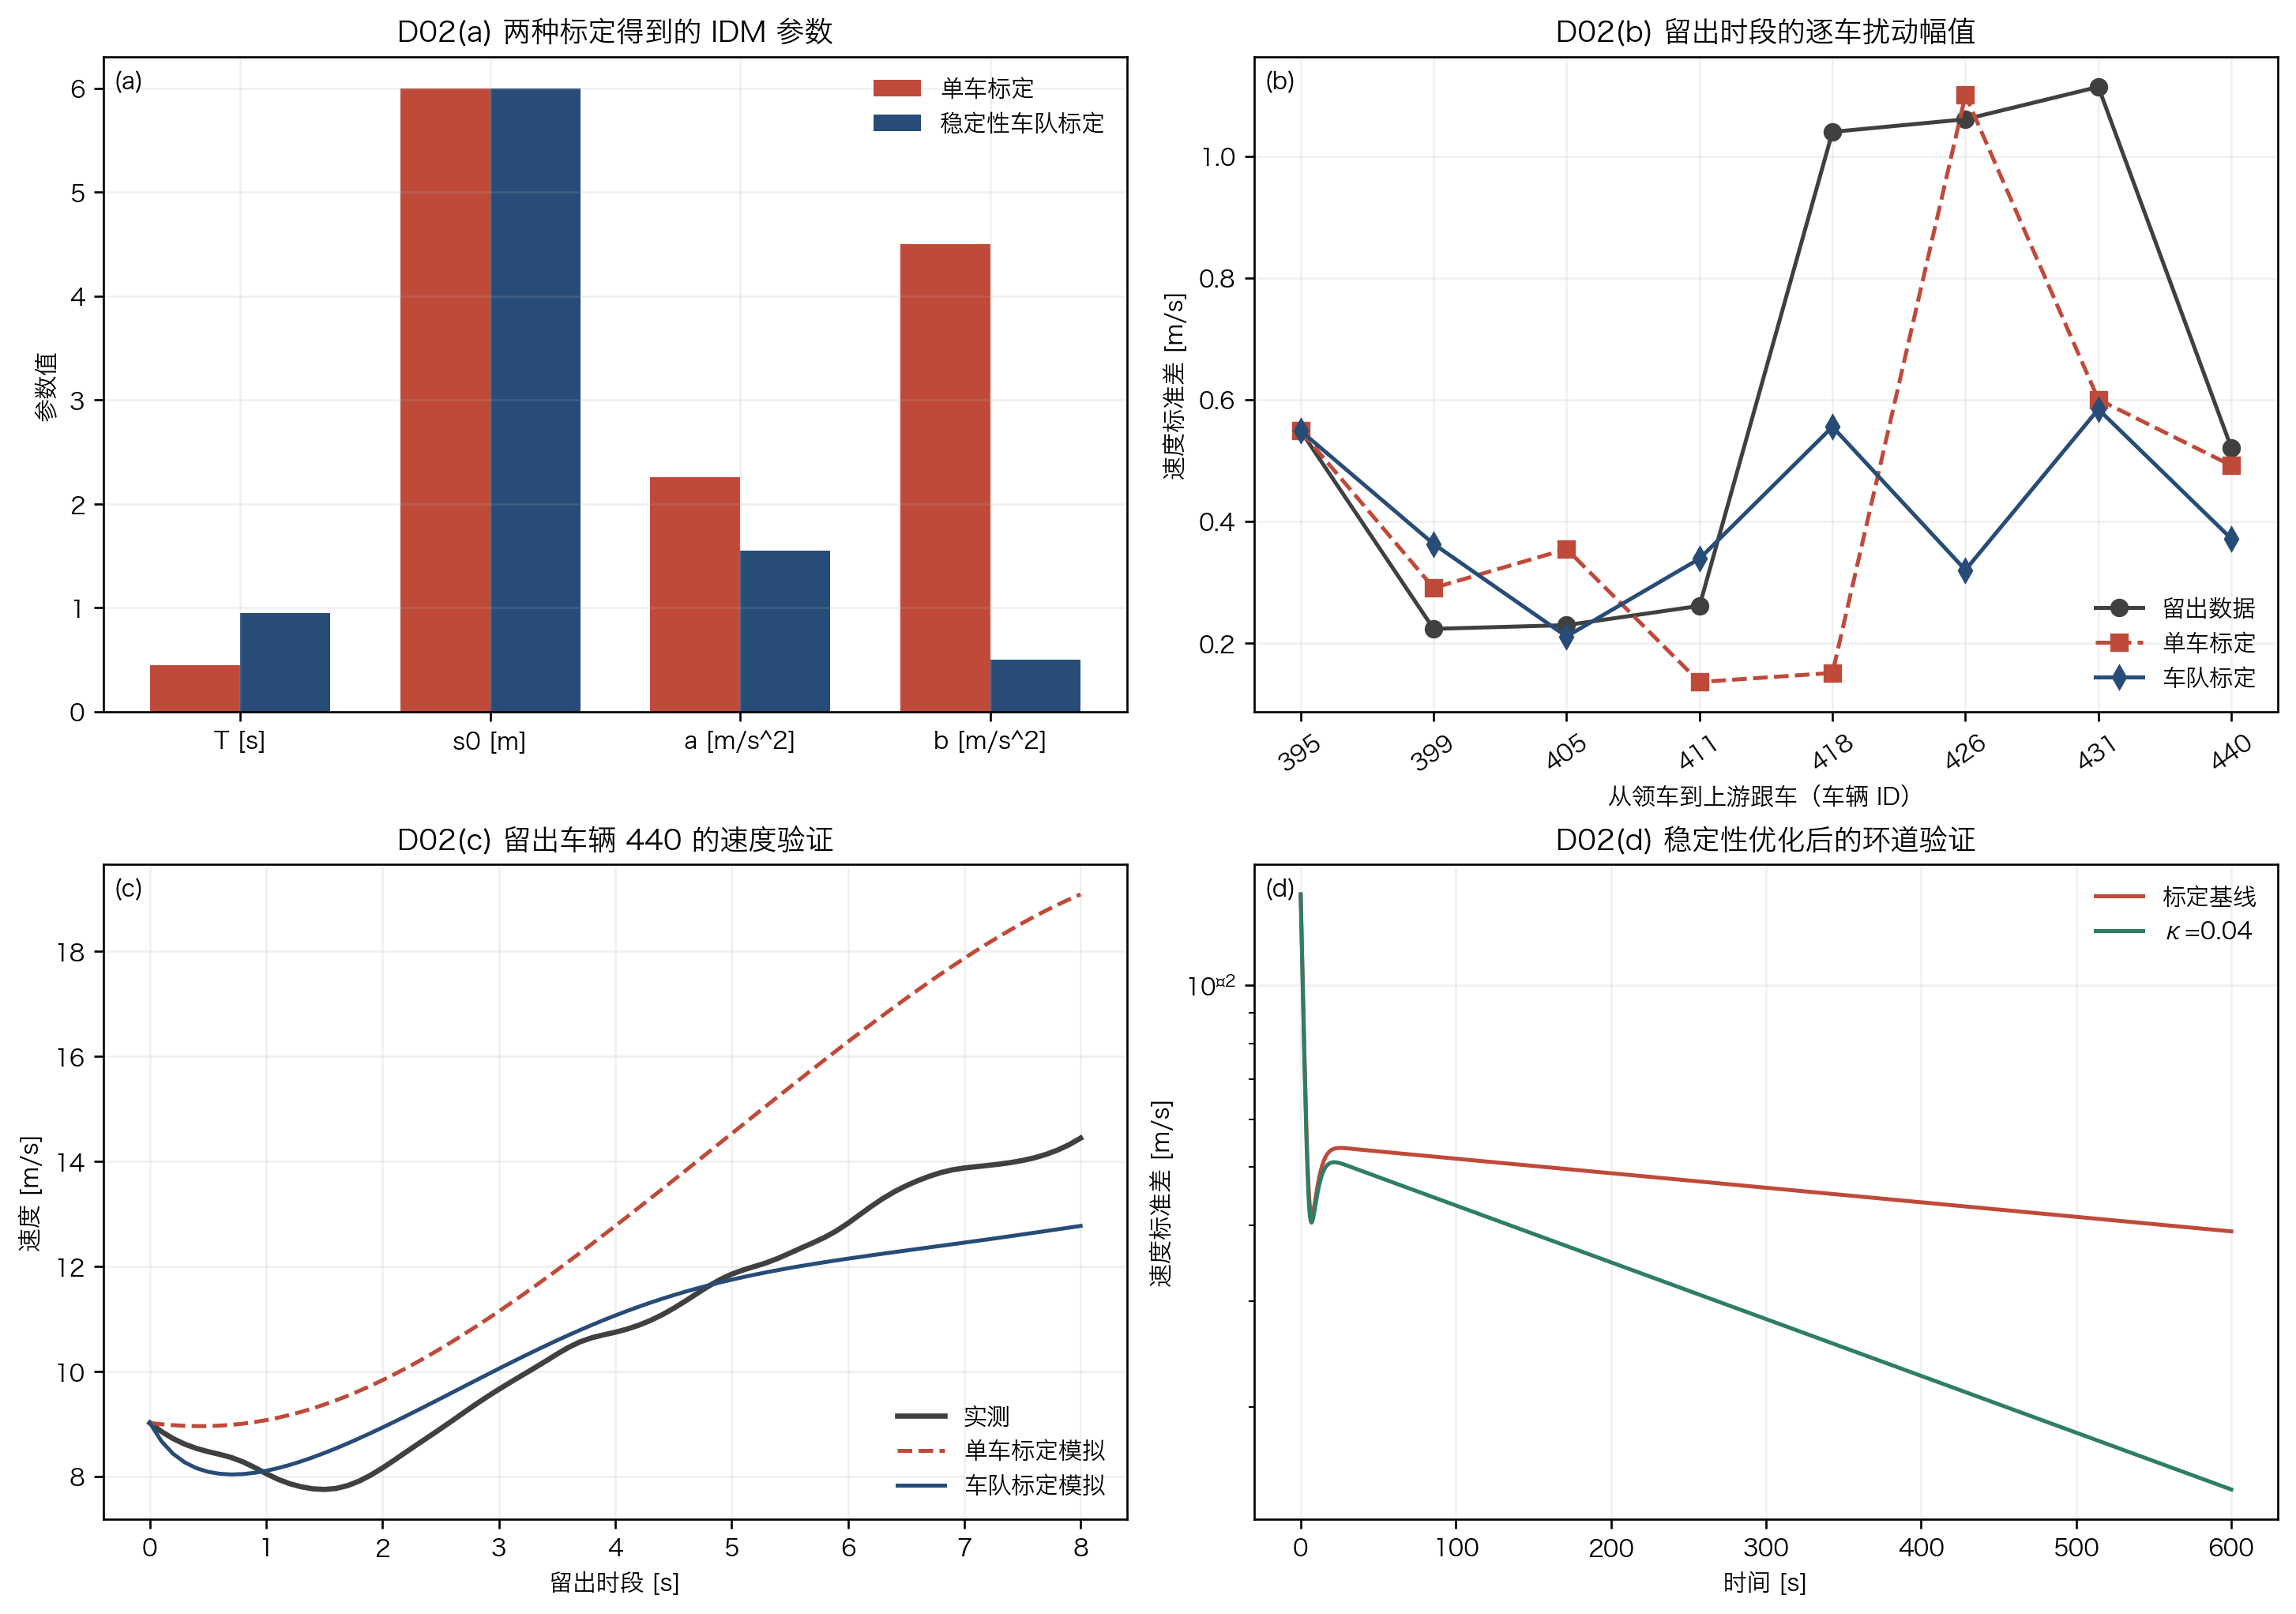
\includegraphics[width=\textwidth]{ngsim_stability_application_d02.png}
\caption{NGSIM 的稳定性标定、验证与控制评估。}
\label{fig:ngsim-d02}
\figurenote{D02 将真实数据用于稳定性标定、留出验证和控制设计的三阶段示范。面板 (a) 比较只拟合第一辆跟车与同时约束七辆车轨迹及幅值剖面的参数结果；后者更好保持车队内部扰动形状，说明稳定性信息会实质改变 IDM 参数，而不是给同一 RMSE 换一个名称。面板 (b) 在完全留出的 8 s 时段比较逐车幅值，面板 (c) 展开最上游车辆 440 的递推速度；车队标定显著减小速度和间距漂移，但并未改善每一项传播统计量，揭示短留出窗的证据边界。面板 (d) 冻结标定参数，在第 5 百分位危险速度上用谱约束选出最小干预 $\kappa=0.04$，环道残余扰动明显降低。该图证明稳定性可以进入模型标定和控制器选择，但控制收益仍是标定模型上的反事实，不能替代受控道路实测。}
\end{figure}

\begin{tcolorbox}[resultbox,title=\textbf{D02 三块工作应怎样读}]
\textbf{标定}说明车队传播信息会改变参数；\textbf{留出验证}说明这种改变是否能泛化；
\textbf{稳定性优化}说明如何把谱约束变成控制选择。只有前两块直接受到真实跟车观测约束，
第三块的控制收益是模型反事实，必须再由受控道路或试验场数据验证。
\end{tcolorbox}

\section{代码、派生数据与溯源}
\sectionstudy{data}{代码、派生数据与溯源}{ngsim2016,thiemann2008,krajewski2018}

D01 的完整入口为 \texttt{examples/analyze\_ngsim\_us101.py}；D02 的标定、递推模拟、谱优化和作图入口为 \texttt{examples/ngsim\_stability\_application.py}。前者保存官方数据集 DOI、API 字段、时间区间、单位转换、滤波窗口和随机种子，后者读取固定的八车队派生表并输出 \texttt{ngsim\_stability\_application\_d02.json} 与图~\ref{fig:ngsim-d02}。原始全数据不受本书代码许可证重新授权；开源包只保留查询脚本和小型派生结果。执行命令与目录说明见附录~\ref{sec:open-code}。

%==================================================================
\sectionwrapup{D01 从 NGSIM 真实轨迹提取 78 个自然跟驰事件，中位增益 1.033 且 95\% 区间跨过 1。D02 进一步完成稳定性车队标定、留出递推模拟和谱约束优化：车队标定显著降低留出速度／间距误差，但并未改善全部传播指标；$\kappa=0.04$ 的控制收益属于标定模型反事实，仍需受控实测验证。}

\chapter{稳定性分析的应用}
\label{sec:applications}
\chapterguide{稳定性判据怎样转化为交通管理与控制设计}{本章用开放车队协同 AV 和固定上游 VSL 两个完整案例，把稳定域、增益、渗透率和传播速度转化为控制选择；安全、效率与能耗则作为仿真后评价，避免混入在线稳定性目标。}

稳定性分析的价值不只是给参数画一条“稳定／不稳定”分界线。它把车辆参数、控制器、通信延迟、车队组成和试验规模转化为可测量的增长率、放大率、主导波长和恢复时间，从而服务于设计、运行、标定与验证。

\section{具体案例 A：开放车队的扰动传播与协同 AV}
\sectionstudy{application}{具体案例 A：开放车队的扰动传播与协同 AV}{milanes2014,talebpour2016,stern2018}
\label{sub:application-open-platoon}

先考虑一个可直接对应道路跟驰试验的开放边界车队。共有 $N=60$ 辆车，均匀初始速度为 $v_e=8$ m/s，初始净间距取 IDM 平衡值。头车在 $t=100$ s 开始施加
\begin{equation}
v_0(t)=v_e+0.6\sin\!\left[\frac{2\pi(t-100)}{48}\right],
\qquad 100\le t\le340\ {\rm s},
\label{eq:application-leader-sine}
\end{equation}
即振幅 $0.6$ m/s、周期 $48$ s、持续 5 个周期的有限时长正弦扰动。这个频率接近该工况传递增益的峰值，所以基准 HDV/IDM 车队会把扰动向上游放大；扰动结束以后，车辆还需一段时间才能回到均匀流。

协同 AV 对照组使用三前车加速度前馈和一后车速度反馈：
\begin{equation}
\dot v_n
=F_n+\sum_{j=1}^{3}\kappa\alpha^{j-1}\dot v_{n-j}
+\gamma\sum_{j=1}^{3}\alpha^{j-1}(v_{n-j}-v_n)
+\eta(v_{n+1}-v_n),
\label{eq:application-cooperative-av}
\end{equation}
其中 $\kappa=0.34$、$\alpha=0.52$、$\gamma=0.045$、$\eta=0.055$；边界处只保留实际存在的邻车。这个控制器代表“多前车信息提前预见扰动，后车信息抑制车队内部速度离散”的通信场景。它并不改变头车输入，因此两组的差异可以归因于扰动传播性质，而不是外部需求不同。

\begin{center}
\small
\captionof{table}{案例 A 的协同 AV 稳定性收益。}
\label{tab:application-av-benefits}
\begin{tabular}{p{4.2cm}rrp{4.4cm}}
\toprule
\textbf{指标} & \textbf{HDV/IDM} & \textbf{协同 AV} & \textbf{稳定性收益} \\
\midrule
末车速度振幅 [m/s] & $0.927$ & $0.099$ & 下降 $89.3\%$；传播增益由 $1.545$ 降至 $0.165$ \\
峰值速度标准差 [m/s] & $0.549$ & $0.193$ & 下降 $64.9\%$ \\
恢复时刻 [s] & $454$ & $392$ & 提前 $62$ s \\
最小净间距 [m] & $12.59$ & $13.11$ & 间距裕量增大 \\
最小 TTC [s] & $65.3$ & $116.2$ & 小扰动安全代理提高 $78.0\%$ \\
Wu 模型扰动附加电耗 [Wh/车] & $0.718$ & $0.076$ & 下降 $89.4\%$ \\
单位里程净电耗 [kWh/100 km] & $4.412$ & $4.405$ & 下降 $0.15\%$ \\
\bottomrule
\end{tabular}
\end{center}
\tabletext{tab:application-av-benefits}{同一头车正弦扰动下纯 HDV 与协同 AV 车队的传播、恢复、安全代理和能耗结果。末车振幅与扰动附加电耗均下降约 $89\%$，而总单位里程电耗只小幅变化，说明稳定控制主要消除反复加减速造成的边际损失。}

为避免把 $v\max(\dot v,0)$ 误当成真实能耗，本书采用 Wu 等人基于实车数据验证的 EV 瞬时功率模型\cite{wu2015ev}。在速度 $v$、加速度 $a$、坡度 $\theta$ 下，先写牵引力
\begin{equation}
F_{\rm tr}=ma+kv^2+f_{\rm rl}mg+mg\sin\theta,
\label{eq:wu-tractive-force}
\end{equation}
电池侧功率写成
\begin{equation}
P_{\rm EV}
=\frac{rR^2}{K^2}F_{\rm tr}^{\,2}
+v\!\left(kv^2+f_{\rm rl}mg+mg\sin\theta\right)+mav,
\qquad
E_{\rm EV}=\int_0^{T_f}P_{\rm EV}(t)\,{\rm d}t.
\label{eq:wu-ev-power}
\end{equation}
第一项为电机铜耗，第二项为克服空气、滚动和坡度阻力所需的功率，第三项为动能变化；$P_{\rm EV}<0$ 表示再生制动回充。算例取该文表~1 的实车参数：$m=1266$ kg、$f_{\rm rl}=0.006$、$k=1.30$ kg/m、$K=10.08$ V$\cdot$s、$r=0.11\ \Omega$、$R=0.50$ m，并令 $\theta=0$。这里的绝对电耗对应 Wu 等人的改装试验车，不能直接冒充任意量产 EV；原文 41 次行程的平均绝对误差为 $15.6\%$，因此本书主要使用同车、同路、同时间窗下的相对变化。

“扰动附加电耗”定义为完整轨迹电耗减去同一车辆以 $v_e=8$ m/s 匀速行驶 1200 s 的电耗。HDV 与 AV 的平均速度几乎相同，总单位里程电耗只相差 $0.15\%$；但与反复加减速直接相关的附加电耗从 $0.718$ 降到 $0.076$ Wh/车，下降 $89.4\%$。这一区分很重要：稳定控制显著消除了\cnemph{扰动造成的边际损失}，却不会消除维持基准巡航所需的主体能量。TTC 数值也处于非危险区，它说明的是相对安全裕量改善；若要评价碰撞风险，应改用更强制动幅值并加入制动饱和与感知误差。

\begin{figure}[htbp]
\centering
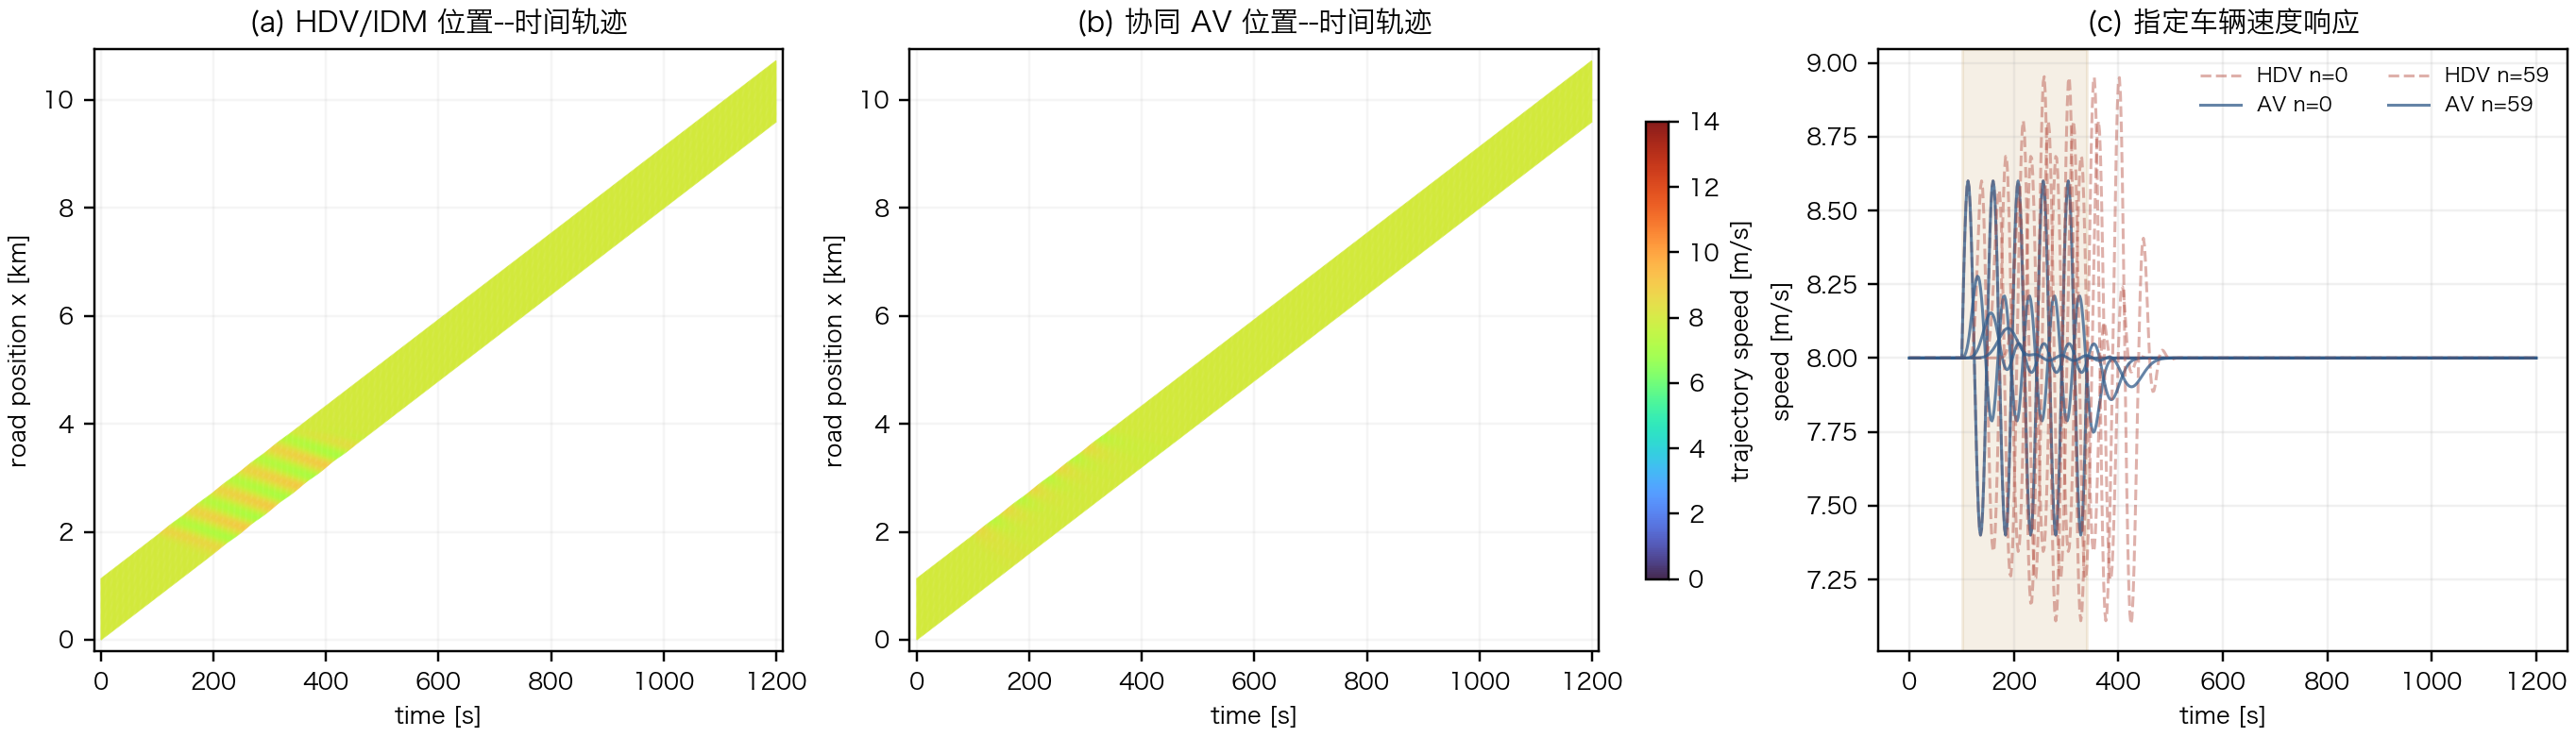
\includegraphics[width=\textwidth]{application_open_platoon.png}
\caption{案例 A：开放车队中的协同 AV 稳定化。}
\label{fig:application-open-platoon}
\figurenote{案例 A 展示同一开放车队输入在纯 HDV 与协同 AV 下的不同传播后果。头车从 $t=100$ s 起施加振幅 0.6 m/s、周期 48 s、共 5 个周期的正弦扰动，之后恢复匀速；左、中的位置--时间图使用同一速度色标，因而可以直接比较有色波带沿实际道路坐标的宽度和持续时间。纯 HDV 中波带向上游车辆逐车加宽，即使头车输入停止后仍保留明显余振；协同 AV 利用多前车预见和后车速度反馈使波带收窄，并较快恢复为颜色均匀的斜直轨迹。右侧指定车辆曲线进一步显示末车振幅由 0.927 降至 0.099 m/s，传播增益由 1.545 降至 0.165，恢复时刻提前 62 s。结合表~\ref{tab:application-av-benefits}，该图证明稳定技术减少的不只是视觉上的波动，还同步降低速度离散、扰动附加电耗并提高间距代理；但这些安全和能耗收益是仿真后评价，不是线性判据单独保证的结果。}
\end{figure}

\section{具体案例 B：连续车流中的低速车辆与固定空间可变限速区}
\sectionstudy{application}{具体案例 B：连续车流中的低速车辆与固定空间可变限速区}{hegyi2005,carlson2010}
\label{sub:application-moving-bottleneck}

第二个案例使用连续开放交通流，并保留高速公路法定最高限速 $120$ km/h。为按读者建议构造一个真正的线性失稳高速工况，本书只把 IDM 期望车头时距从基准值减小到 $T=0.7$ s；其余 IDM 参数保持不变。取净间距 $s_e=18$ m、车长 $l=5$ m 时，$v_0=120$ km/h 对应的均匀平衡速度为 $v_e=74.95$ km/h，流率约为 $3261$ veh/h。这个流率高于常规人工驾驶单车道能力，因而应理解为一个\textbf{短时距、高需求的理论验证工况}，而不是普通 HDV 容量标定。$0$--$1200$ s 内车辆持续进入并从下游驶出，共有 1087 辆新车越过上游边界。

编号 533 的车辆在 $t=300$ s 到达约 $x_b=6$ km 处，并在 $300$--$420$ s 把目标速度从约 $75$ km/h 降至 $18$ m/s（$64.8$ km/h）。这只是约 $10$ km/h 的有限时长扰动；但由于小 $T$ 工作点满足 $\Phi<0$，扰动会被放大并形成明显向上游传播的排队尾波。这样可以把“稳定性导致的放大”与“极端事故直接封路”区分开来。

VSL 不是对“所有上游车辆”统一改参数，也不跟随慢车移动。它固定布设在慢车开始降速的位置 $x_b^0=6$ km 的上游 1 km：
\begin{equation}
\Omega_{\rm VSL}=\bigl[x_b^0-1000,\ x_b^0\bigr)
= [5000,6000)~{\rm m},
\qquad 300\le t\le900~{\rm s}.
\label{eq:vsl-fixed-zone}
\end{equation}
车辆只有在自身位置 $x_n(t)\in\Omega_{\rm VSL}$ 时才接受限速命令。更重要的是，$t<300$ s 时 VSL 严格关闭；慢车于 $t=300$ s 开始降速后，路侧检测才触发控制，因而本算例不再包含任何预见事故的提前限速。慢车离开 6 km 事件点以后，VSL 仍留在 5--6 km 固定路段；它既不绑定车辆编号，也不沿慢车轨迹平移。图~\ref{fig:application-moving-bottleneck}(f) 同时画出慢车轨迹与固定空间带，二者在事件发生后逐渐分离。

\subsection{在允许范围内直接最大化稳定裕度}

道路管理界面显示的 VSL 目标记为 $u$，本算例直接令 IDM 期望速度参数 $v_0=u$；道路法定上限仍是 $120$ km/h。固定当前净间距 $s_e=18$ m，对每个运营允许目标 $u\in\mathcal U=[114,120]$ km/h，先求新的均匀平衡速度 $v_e(u)$：
\begin{equation}
F\!\left(s_e,v_e(u),0;v_0=u,T=0.7~{\rm s}\right)=0,
\label{eq:vsl-new-equilibrium}
\end{equation}
再在该新平衡点计算长波裕度
\begin{equation}
\Phi(u)=\frac12\left[f_v(u)^2-f_{v_l}(u)^2\right]-f_s(u).
\label{eq:vsl-phi}
\end{equation}
允许范围 $\mathcal U$ 是管理者事先给定的在线控制约束；在该范围内，目标函数只包含\textbf{稳定性量}：
\begin{equation}
u^*=\arg\max_{u\in\mathcal U}\Phi(u).
\label{eq:vsl-stability-only-objective}
\end{equation}
这里不再选择“刚好超过阈值”的最小裕度，而是在允许速度带内直接取最大的 $\Phi$。最小 TTC、排队、延误或能耗均没有进入式~\eqref{eq:vsl-stability-only-objective}；这些指标只能在控制值确定后由完整仿真事后评价。

\begin{center}
\small
\captionof{table}{VSL 候选速度的稳定裕度。}
\label{tab:vsl-candidates}
\begin{tabular}{rrrr}
\toprule
$u$ [km/h] & $v_e(u)$ [km/h] & $\Phi(u)$ [s$^{-2}$] & 线性结论 \\
\midrule
\textbf{114} & \textbf{73.78} & \textbf{$+0.002396$} & \textbf{稳定，裕度最大} \\
115 & 73.98 & $+0.001727$ & 稳定 \\
116 & 74.19 & $+0.001071$ & 稳定 \\
117 & 74.39 & $+0.000429$ & 稳定 \\
118 & 74.58 & $-0.000199$ & 失稳 \\
119 & 74.77 & $-0.000814$ & 失稳 \\
120 & 74.95 & $-0.001415$ & 失稳 \\
\bottomrule
\end{tabular}
\end{center}
\tabletext{tab:vsl-candidates}{114--120 km/h 运营允许带内各候选限速重新求得的平衡速度与解析裕度。$u=118$ km/h 起裕度转负，而 $u=114$ km/h 在可行集合内给出最大正裕度，因此控制量来自稳定性优化而非事后安全或延误指标。}

无控制时，法定上限 $u=120$ km/h 对应 $\Phi=-0.001415$ s$^{-2}$，确实处在线性失稳侧。最大化式~\eqref{eq:vsl-stability-only-objective} 得到 $u^*=114$ km/h，$\Phi=+0.002396$ s$^{-2}$，只降低 $6$ km/h 便使工作点跨入稳定侧。$114$ km/h 的下界是对一公里控制区预先给定的运营约束，不是用安全或延误仿真反推出来的。事件与控制在 $t=300$ s 同时触发，命令在 $300$--330$ s 平滑进入、在 $810$--900$ s 平滑退出；车辆在固定 5--6 km 区内沿空间渐变适应目标速度，以避免入口处人为制造阶跃冲击。这里的“同时触发”表示理想化的即时检测；若要研究通信与检测滞后，应另设正的触发延迟并重新仿真，而不能把控制提前到事件之前。

\subsection{仿真后评价：不能反过来冒充在线目标}

为直接测量传播方向，定义低速排队尾部
\begin{equation}
x_q(t)=\min\{x_n(t):v_n(t)<18.2~{\rm m/s}\},
\qquad c_q=\frac{{\rm d}x_q}{{\rm d}t}.
\label{eq:vsl-queue-tail-speed}
\end{equation}
$c_q<0$ 表示尾部向上游传播。本书在 $360$--$420$ s 的线性段拟合 $c_q$。其余排队、安全、延误与能耗也全部由两次完整连续流仿真\textbf{事后计算}，没有进入式~\eqref{eq:vsl-stability-only-objective}。

\begin{center}
\small
\captionof{table}{案例 B 的 VSL 事后评价。}
\label{tab:vsl-post-evaluation}
\begin{tabular}{p{4.2cm}rrp{4.4cm}}
\toprule
\textbf{指标} & \textbf{无控制} & \textbf{稳定性约束 VSL} & \textbf{结果} \\
\midrule
1200 s 内新到达车辆 & $1087$ & $1087$ & 两组边界需求完全相同 \\
驶出下游车辆 & $1072$ & $1072$ & 两组相同 \\
形成阶段排队尾波速度 $c_q$ [m/s] & $-2.687$ & $-0.284$ & 逆向传播速度绝对值下降 $89.4\%$ \\
低速车辆峰值（$v<18.2$ m/s） & $121$ & $102$ & 下降 $15.7\%$ \\
峰值速度标准差 [m/s] & $8.912$ & $4.107$ & 下降 $53.9\%$ \\
最小净间距 [m] & $1.56$ & $3.27$ & 提高约 $109.8\%$ \\
最小 TTC [s] & $2.34$ & $6.70$ & 提高约 $186\%$ \\
累计延误 [veh$\cdot$h] & $6.866$ & $4.799$ & 下降 $30.1\%$ \\
单位里程净电耗 [kWh/100 km] & $17.521$ & $17.328$ & 下降 $1.10\%$ \\
\bottomrule
\end{tabular}
\end{center}
\tabletext{tab:vsl-post-evaluation}{相同连续到达需求下无控制与事件触发型 VSL 的完整仿真结果。控制在慢车扰动发生前保持关闭；触发后负尾波速度的绝对值下降 $89.4\%$，同时排队规模、速度离散、延误和安全代理改善。这些数值用于验证由 $\Phi$ 选出的限速，而没有反向参与在线目标。}

无控制位置--时间图中的黑色虚线从 $x=6$ km 明显向较小的 $x$ 倾斜；在 $360$--$420$ s 形成阶段拟合得 $c_q=-2.687$ m/s，明确证明拥堵尾波向上游传播。事件触发型 VSL 在 $t=300$ s 之前不改变任何车辆，触发后才把上游工作点从 $\Phi<0$ 推向 $\Phi>0$。控制图中的低速色带明显收窄，形成阶段尾部斜率绝对值减小到 $0.284$ m/s；峰值速度离差下降 $53.9\%$，累计延误下降 $30.1\%$，最小 TTC 从 $2.34$ s 提高到 $6.70$ s。与含预控制的旧结果相比，收益有所减弱但因果顺序正确。仍需强调：\textbf{只有 $\Phi$ 进入在线目标；尾波速度、排队、安全、延误和能耗全部是事后验证结果，而不是理论预先保证。}

\begin{figure}[htbp]
\centering
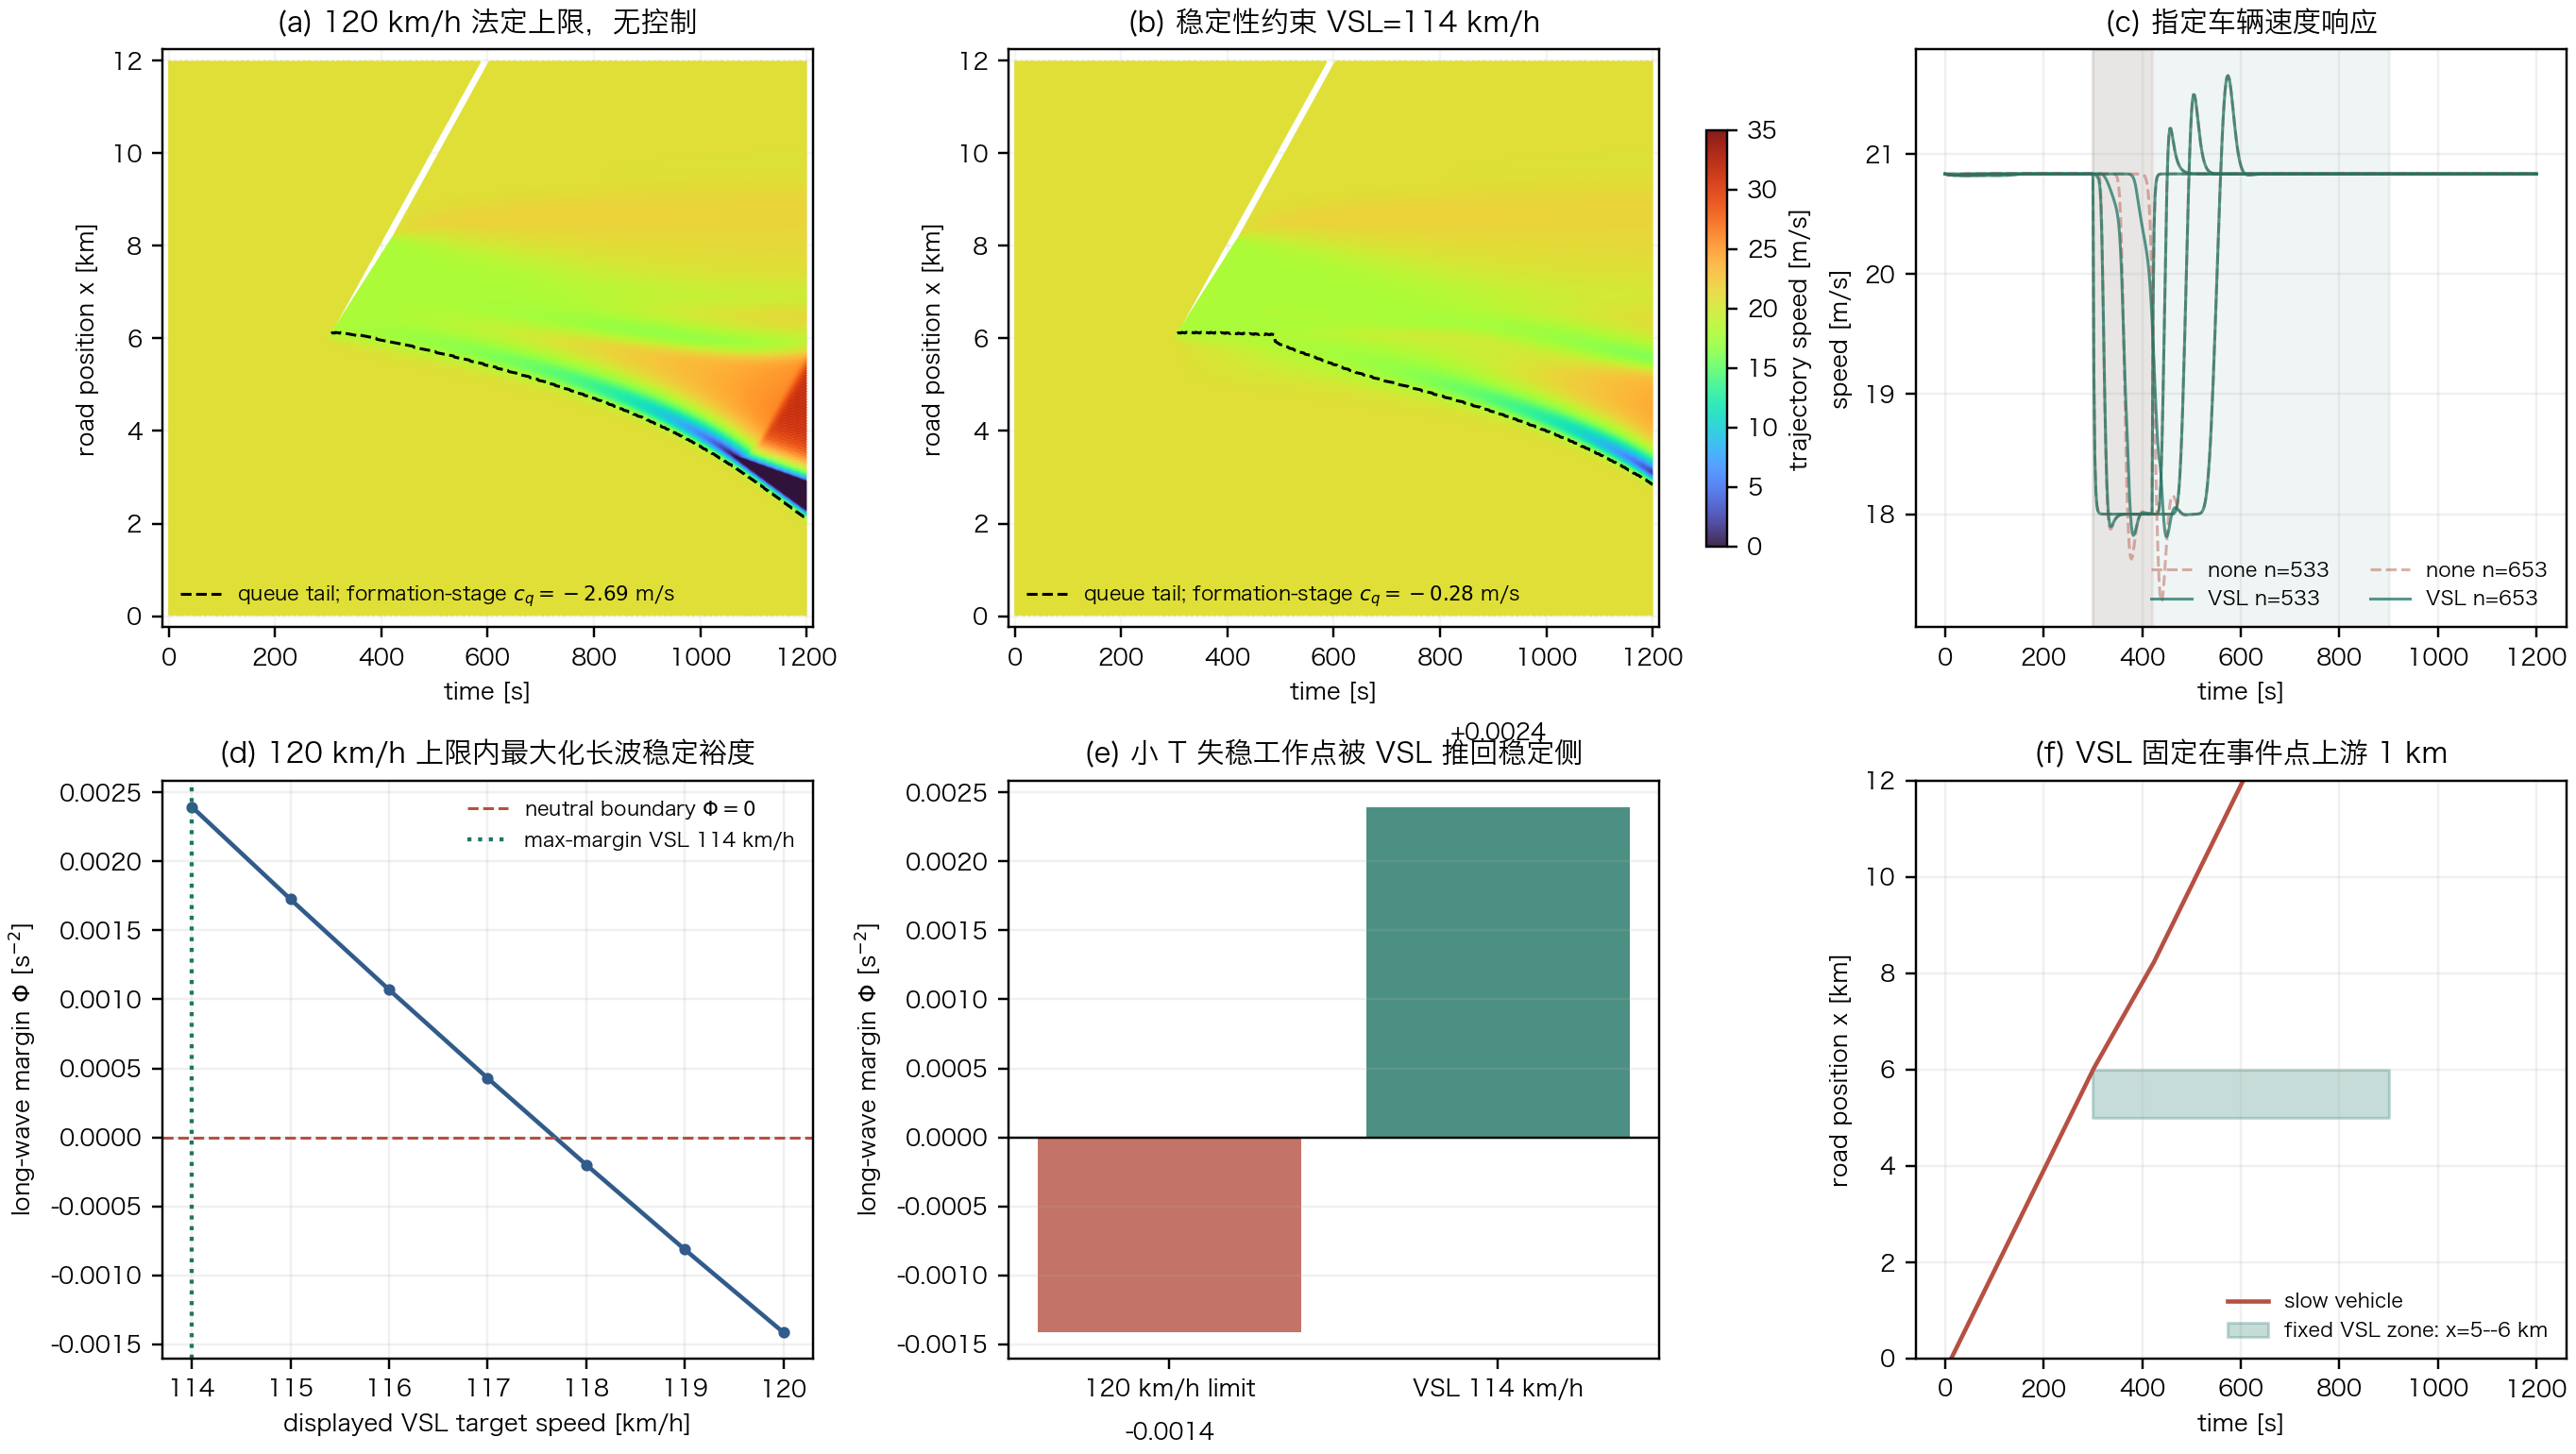
\includegraphics[width=\textwidth]{application_moving_bottleneck.png}
\caption{案例 B：基于最大稳定裕度的固定区域 VSL。}
\label{fig:application-moving-bottleneck}
\figurenote{案例 B 展示稳定性约束如何转化为固定空间、事件触发型 VSL，并用完整连续流仿真验证其道路效益。$0$--$1200$ s 内上游需求持续到达，法定最高限速保持 120 km/h；短时距 $T=0.7$ s 使均匀流处于 $\Phi<0$，编号 533 的慢车在 $t=300$ s、$x=6$ km 附近触发扰动。$t<300$ s 时 VSL 严格关闭；随后固定 $x=5$--$6$ km 的控制带才出现，并不跟随慢车。无控制图中的低速尾部向较小 $x$ 倾斜，拟合速度 $c_q=-2.687$ m/s。候选限速只在 114--120 km/h 内比较解析裕度，$u^*=114$ km/h 使 $\Phi$ 由 $-0.001415$ 变为 $+0.002396$。触发后控制图中的低速色带收窄，尾波速度绝对值降至 0.284 m/s；表~\ref{tab:vsl-post-evaluation} 显示速度离散下降 53.9\%、累计延误下降 30.1\%。该图说明稳定性约束仍可在没有预控制的条件下减弱扰动放大，而排队、安全、延误和电耗只是控制值确定后的事后证据。}
\end{figure}

\begin{tcolorbox}[resultbox,title=\textbf{两个案例说明稳定性分析怎样帮助交通管理}]
\begin{itemize}[leftmargin=1.4em,itemsep=3pt]
\item 对车端控制，线稳定性给出“扰动会不会逐车放大”的前置筛选；时域仿真再把谱裕度换算成安全间距、恢复时间和 Wu 模型电耗。
\item 对路侧管理，每个候选限速都要重新求平衡点与稳定域；在线目标函数只使用稳定裕度 $\Phi$，位置--时间轨迹、队列、安全、延误和能耗再作为事后检验。
\item 控制评价必须同时报告收益与代价。只展示更平滑的速度颜色图，而不报告延误、恢复和能耗，可能把“把拥堵暂时存到上游”误写成“消除拥堵”。
\end{itemize}
实验台的“应用案例”页签提供两组无控制／控制位置--时间轨迹、指定车辆速度曲线、VSL 扫描与上述量化读数，可逐项对应图~\ref{fig:application-open-platoon} 和图~\ref{fig:application-moving-bottleneck}。
\end{tcolorbox}

\section{应用一：ACC／CACC 控制器的增益设计}
\sectionstudy{application}{应用一：ACC／CACC 控制器的增益设计}{milanes2014,talebpour2016,stern2018}

控制设计应按“长波预算 $\rightarrow$ 全频段约束 $\rightarrow$ 时域验证”的顺序进行。对前车加速度前馈，第一步由
\begin{equation}
\kappa_{\min}(v_e)
=1-\frac{f_v^2-f_{v_l}^2}{2f_s}
\label{eq:application-kappa}
\end{equation}
给出工作点所需的最低增益，再检查 $|\kappa|\le1$ 与通信延迟下的 $\Psi(\omega)\ge0$。本书基准 IDM 的全速域最坏值为 $\kappa_c=0.134$，所以选择 $\kappa=0.15$ 已能把 $v_e=8$ m/s、$m=4$ 的增长率从 $+0.00408566$ s$^{-1}$ 变为最右模态 $-1.14052\times10^{-4}$ s$^{-1}$。前者的线性倍增时间仅
\begin{equation}
t_2=\frac{\ln2}{0.00408566}=169.7\ \text{s},
\end{equation}
意味着约三分钟内扰动即可翻倍；稳定化后则转为缓慢衰减。

工程上不能只取“刚过临界”的增益。若 $\kappa$ 太接近 $0.134$，参数误差、采样延迟和车型差异都可能吃掉裕度；若 $\kappa$ 过大，又会靠近高频上界。合理做法是在速度--密度工作域上最大化最小谱裕度，同时加入加速度、舒适度和执行器带宽约束。

\section{应用二：混合交通的 AV 渗透率与编组部署}
\sectionstudy{application}{应用二：混合交通的 AV 渗透率与编组部署}{milanes2014,talebpour2016,stern2018}

异质车队的长波指数 $\eta_n$ 可直接转化为渗透率预算。本书在 $\kappa=0.5$ 时得到整队／环道长波总预算门槛 $26.7\%$；它只保证 $S_N\ge0$，开放车队仍须检查全部 $S_j$。当 AV 只有在前车也是 AV 时才能获得完整 V2V 前馈，\textbf{同一渗透率的排列还会改变总稳定预算}。$N=120$、30\% AV、$v_e=9$ m/s 时，闭式结果给出 $n_{\rm grp}^{\max}=5.6$：最多分成 5 组才能先保证总预算，再在这个约束下尽量均匀布置以降低中途峰值。

这类结论可用于车队编组、专用车道入口排序和协同巡航激活策略：先保证足够多的 AV--AV 相邻对，再优化车辆分散程度，而不是只报告一个与排列无关的“平均渗透率”。

工程部署还应使用图~\ref{fig:av-stability-plane} 的 $p_{\rm AV}$--$v_e$ 二维稳定域，而不是把 $26.7\%$ 当成所有速度、所有排列都通用的常数。实际流程是在目标速度带内读取最不利边界，并对 $\kappa_0$、编组数和排列不确定性留出正的 $M_{\rm L}$ 与 $M_{\rm T}$ 裕度。

\section{应用三：在线拥堵预警与控制触发}
\sectionstudy{application}{应用三：在线拥堵预警与控制触发}{milanes2014,stern2018,hegyi2005}

实际运行中可在滚动时间窗内计算速度离差和主导 Fourier 模态：
\begin{equation}
\widehat g(t)=\frac{\mathrm d}{\mathrm dt}\ln\sigma_v(t),
\qquad
\widehat m^*(t)=\arg\max_m|A_m(t)|.
\label{eq:online-indicators}
\end{equation}
若 $\widehat g$ 持续为正、主导模态在相邻窗口保持一致，而且幅值仍处于线性区，就可以在完全走停波形成前触发控制。第~\ref{sec:protocol}~章的在线干预算例在 $t=600$ s 开始把 $\kappa$ 从 0 平滑升至 0.45，速度标准差由形成后的约 $0.534$ m/s 降到 $0.018$ m/s，说明稳定性指标不仅能做离线判据，也能成为在线触发量。

为了避免把一次孤立制动误判成自激失稳，预警至少应同时满足三个条件：增长率为正、空间模态具有持续性、扰动在多个车辆之间传播；单点速度下降本身不够。

\section{应用四：环道试验与仿真规模设计}
\sectionstudy{application}{应用四：环道试验与仿真规模设计}{milanes2014,stern2018,hegyi2005}

有限环道的最低波数为 $2\pi/N$。若研究目标是估计无限车队的线稳定边界，试验规模必须覆盖危险长波。本书基准算例中，$N=22$ 只能观察到 $1.45$--$11.43$ m/s 的不稳定带，而连续极限为 $0.91$--$18.61$ m/s；$N=100$ 才扩展到 $0.93$--$18.35$ m/s。因此：
\begin{itemize}[leftmargin=1.4em,itemsep=3pt]
\item 小环道适合演示波的形成与传播，却不适合直接标定无限车队阈值；
\item 若车辆数受限，应使用有限 $N$ 的闭式条件而不是连续极限公式；
\item 实验报告必须给出 $N$、环长、允许波数 $k_m$ 和被激发的模态，不能只写密度。
\end{itemize}

\section{应用五：模型标定与模型选择}
\sectionstudy{application}{应用五：模型标定与模型选择}{kesting2008,ossen2009,punzo2012}

只用均方根速度误差标定跟驰模型，可能得到“单车轨迹拟合很好、车队稳定性完全错误”的参数。更可靠的目标函数应同时包含：
\begin{equation}
J(\theta)=w_1J_{\rm traj}+w_2J_{\rm local}+w_3J_{\rm gain}+w_4J_{\rm wave},
\label{eq:calibration-objective}
\end{equation}
其中 $J_{\rm traj}$ 衡量位置／速度轨迹误差，$J_{\rm local}$ 衡量单车根，$J_{\rm gain}$ 衡量车对车放大率或增长率，$J_{\rm wave}$ 衡量波速与主导波长。用独立试验验证 $\operatorname{Re}\lambda(k)$ 和 $|G(i\omega)|$，可以排除那些虽然逐点拟合好、却会产生虚假走停波或过度耗散的参数组。

数值格式也应作为“模型的一部分”接受验证：同一工况用 $\Delta t$ 和 $\Delta t/2$ 重算，若增长率或临界点明显变化，说明观测到的是离散化稳定性而不是车辆模型稳定性。

\section{应用六：运行策略、容量与舒适性的权衡}
\sectionstudy{application}{应用六：运行策略、容量与舒适性的权衡}{milanes2014,stern2018,hegyi2005}

稳定性裕度可用于速度建议、时距管理和道路运行分区。增大 IDM 的期望时距 $T$ 往往提高稳定性，但会降低容量；增大加速度前馈可保持较小 $T$，却增加对通信可靠性与执行器带宽的要求；后向间距反馈能同时降低波速，却引入双向耦合与有限波长约束。因此设计目标不应是单独最大化稳定性，而应求解
\begin{equation}
\max_{\theta}\ \min_{(v_e,\rho)\in\Omega}M_\lambda(\theta;v_e,\rho)
\quad\text{s.t.}\quad
q\ge q_{\min},\ |a|\le a_{\max},\ |j|\le j_{\max},\ \tau\le\tau_{\max},
\label{eq:robust-design}
\end{equation}
即在目标工作域 $\Omega$ 内最大化最坏稳定裕度，同时满足容量、加速度、加加速度（jerk）和延迟约束。稳定性由此成为多目标设计中的一个可计算指标，而不是孤立的“越大越好”。

\section{从分析到实施的六步流程}
\sectionstudy{application}{从分析到实施的六步流程}{milanes2014,stern2018,hegyi2005}

\begin{tcolorbox}[keybox,title=\textbf{建议的工程工作流}]
\begin{enumerate}[leftmargin=1.6em,itemsep=4pt]
\item \textbf{定工作域：}给出速度、密度、车辆数、车型比例和延迟范围，而不是只选一个名义点。
\item \textbf{查局部根：}先保证每辆车自身稳定，并记录最慢恢复时间与阻尼比。
\item \textbf{查传播：}单向均匀模型用 $|G(i\omega)|$；双向模型扫 $\lambda(k)$；异质车队用传递函数乘积或全矩阵本征值。
\item \textbf{留裕度：}不要把参数放在等号边界上；对标定误差、延迟和渗透率做灵敏度／鲁棒性扫描。
\item \textbf{做有限幅验证：}至少扫描三个扰动幅值并运行到多个线性时间常数，区分慢衰减、非线性饱和与亚临界触发。
\item \textbf{闭环复核：}用速度着色的时空轨迹、速度／间距场和指定探针车曲线共同验证，并执行 $\Delta t$ 收敛检查。
\end{enumerate}
\end{tcolorbox}

\begin{tcolorbox}[notebox,title=\textbf{应用边界}]
本书判据用于纵向单车道跟驰。真实道路上的换道、匝道、信号灯、坡度、感知误差、通信丢包和驾驶人随机性会不断注入外部扰动；“模型线稳定”不等于“道路永不拥堵”，更不等于碰撞安全认证。实际控制器还必须独立满足安全距离、故障降级、执行器饱和与形式化验证要求。
\end{tcolorbox}

\sectionwrapup{稳定性分析可把控制参数转换为增长率、传播速度、恢复时间和可用稳定域。开放车队案例说明协同 AV 可抑制上游放大；固定上游 VSL 案例说明限速应由稳定域与运行约束共同确定，而安全、效率和能耗收益需由独立仿真评价。}

\chapter{延伸讨论：机器学习与深度学习架构下的稳定性分析}
\label{sec:ml-stability}
\chapterguide{学习型模型怎样重新接入经典稳定性理论}{本章讨论机器学习跟驰模型、深度时序模型、多车图网络和强化学习控制器。重点不是介绍网络结构本身，而是说明怎样从学习映射提取平衡态、雅可比、传播增益与可验证证书，并区分训练稳定、预测稳定、交通流稳定和闭环安全。}

机器学习能够从大量轨迹中拟合复杂驾驶行为，但“预测误差小”并不自动意味着“长时间滚动不发散”，更不意味着“扰动沿车队不放大”。另一方面，把所有学习模型强行训练成线稳定，也可能抹去人类驾驶数据中真实存在的走停波。因而机器学习在稳定性分析中的合理角色不是替代动力系统理论，而是把未知动力学、隐状态或控制策略写成可微或可界定的算子，再由稳定性工具检查其时间演化与空间传播。

\section{先问清楚：讨论的是哪一种“稳定”}
\sectionstudy{synthesis}{机器学习语境下四类稳定性的区别}{chen2018neuralode,revay2020contracting,wang2025kidl}

同一个“stable learning”术语至少可能指四件不同的事。

\begin{center}
\small
\captionof{table}{机器学习交通模型中的四类稳定性问题。}
\label{tab:ml-four-stabilities}
\begin{tabular}{p{3.2cm}p{4.2cm}p{6.8cm}}
\toprule
\textbf{层次} & \textbf{典型问题} & \textbf{正确的检查对象} \\
\midrule
训练／优化稳定性 & 损失是否收敛、梯度是否爆炸或消失 & 优化算法、梯度统计与随机种子；不直接给出交通流结论 \\[3pt]
单模型滚动稳定性 & 学习到的速度／加速度模型长时间积分是否有界 & 单步映射或连续向量场的雅可比、吸引域和数值积分器 \\[3pt]
交通流稳定性 & 一个车辆扰动是否随时间或沿车队放大 & 环道模态 $\lambda(k)$、离散步映射 $M(k)$、传递增益与有限幅时空图 \\[3pt]
学习控制器闭环稳定性 & 神经策略接入车辆与交通环境后是否稳定 & \textbf{车辆动力学 $+$ 观测 $+$ 网络策略 $+$ 延迟／采样／饱和}的完整闭环 \\
\bottomrule
\end{tabular}
\end{center}
\tabletext{tab:ml-four-stabilities}{训练过程、单模型滚动、交通扰动传播和学习控制器闭环四个不同层次。只有第三、第四行直接回答本书关心的交通流问题；训练损失平滑或测试集 RMSE 较小不能代替模态与闭环分析。}

还应区分\textbf{模型学习}与\textbf{策略学习}。若网络输出人类驾驶车辆的加速度，它是被研究的跟驰模型；若网络输出 AV 的控制命令，它是闭环中的控制器。前者允许出现数据真实包含的失稳行为，后者通常需要在工作域内主动留出稳定裕度和安全约束。

\section{可微前馈网络：直接用自动微分恢复经典偏导}
\sectionstudy{theory}{由神经跟驰律恢复平衡态与线稳定判据}{wang2025kidl,raissi2019pinn,brunton2016sindy}

最容易分析的学习型跟驰器仍采用本书的三个物理输入：
\begin{equation}
\dot v_n=\widehat F_\theta(s_n,v_n,\Delta v_n),
\qquad \Delta v_n=v_n-v_{n-1},
\label{eq:ml-feedforward-cf}
\end{equation}
其中 $\widehat F_\theta$ 可以是 MLP、核回归、符号回归或“物理模型 $+$ 神经残差”。对给定 $s_e$，平衡速度仍由
\begin{equation}
\widehat F_\theta(s_e,v_e,0)=0
\label{eq:ml-equilibrium}
\end{equation}
数值求解。只要网络在工作点可微，自动微分即可得到
\begin{equation}
\widehat F_s=\frac{\partial \widehat F_\theta}{\partial s},\qquad
\widehat F_v=\frac{\partial \widehat F_\theta}{\partial v},\qquad
\widehat F_{\Delta v}=\frac{\partial \widehat F_\theta}{\partial \Delta v}.
\label{eq:ml-autodiff-partials}
\end{equation}
令 $f_s=\widehat F_s$、$f_v=\widehat F_v+\widehat F_{\Delta v}$、$f_{v_l}=-\widehat F_{\Delta v}$，第~\ref{sec:string}~章的局部根、长波判据与传递函数可以原样复用。特别地，
\begin{equation}
\Phi_\theta(s_e)
=\frac12\left(f_v^2-f_{v_l}^2\right)-f_s
\label{eq:ml-string-margin}
\end{equation}
给出该平衡点的长波稳定裕度；$\Phi_\theta\ge0$ 才通过长波检查，有限频率仍应计算 $|G_\theta(i\omega)|$ 或 $\lambda_\theta(k)$。

这种方法的优势是\textbf{没有必要把网络“解释成 IDM 参数”}：稳定性只需要工作点附近的一阶导数。若希望保留物理结构，可采用
\begin{equation}
\widehat F_\theta=F_{\rm phys}+r_\theta,
\label{eq:ml-hybrid-residual}
\end{equation}
其中 $F_{\rm phys}$ 负责安全距离、自由流极限和平衡基本图，神经残差 $r_\theta$ 只学习系统误差。此时偏导是物理项与残差项偏导之和，既能利用数据，也能检查残差是否把原本稳定的工作点推过中性边界。

ReLU 网络在折点处没有唯一经典导数。若平衡点落在折点附近，不能只接受自动微分框架任意选取的一侧导数；应检查相邻激活区域的雅可比、Clarke 广义雅可比或区间斜率界。采用 $\tanh$、softplus 等光滑激活会让局部推导更直接，但并不自动保证全局稳定。

\section{RNN、LSTM、Neural ODE 与深度平衡网络：必须扩充状态}
\sectionstudy{theory}{含隐状态学习架构的时间稳定性}{chen2018neuralode,bai2019deq,revay2020contracting}

RNN、GRU 或 LSTM 的加速度不仅依赖当前 $s,v,\Delta v$，还依赖隐状态 $h_n$。若数据采样间隔为 $\Delta t$，可统一写成
\begin{equation}
\xi_n^{r+1}=\mathcal M_\theta
\!\left(\xi_n^r,\xi_{n-1}^r,\xi_{n+1}^r\right),
\qquad \xi_n=(s_n,v_n,h_n),
\label{eq:ml-rnn-map}
\end{equation}
其中不存在后车信息时删去第三个输入。平衡态必须同时满足物理状态不变和隐状态不变：
\begin{equation}
\xi_e=\mathcal M_\theta(\xi_e,\xi_e,\xi_e).
\label{eq:ml-hidden-equilibrium}
\end{equation}
这一步不能省略；仅把 $s,v$ 设成常数而随意把 $h$ 清零，可能把隐状态暂态误当成交通失稳。

在均匀环道且参数共享时，对完整映射自动微分可得块矩阵
\begin{equation}
M(k)=M_0+M_-e^{-ik}+M_+e^{ik}.
\label{eq:ml-discrete-symbol}
\end{equation}
因为式~\eqref{eq:ml-rnn-map} 是离散时间系统，稳定条件不是 $\operatorname{Re}\lambda<0$，而是
\begin{equation}
\rho\!\left(M(k)\right)<1
\quad\text{对所有非平凡允许波数 }k,
\label{eq:ml-unit-disk}
\end{equation}
其中 $\rho$ 为谱半径。若使用 Neural ODE，把隐状态写成 $\dot\xi=\mathcal F_\theta(\xi)$，则回到连续时间条件 $\max\operatorname{Re}\lambda(A(k))<0$。Neural ODE 的自适应求解器、RNN 的采样保持和显式 Euler 离散会产生不同的数值稳定域，因此应同时报告学习模型和部署积分器。

深度平衡网络（DEQ）在每个输入下求隐藏层固定点。网络求根器收敛只说明\textbf{特征计算}找到一个隐藏固定点，不等于车辆时间演化或车队传播稳定。必须把 DEQ 对输入的隐式导数接入车辆动力学，再检查闭环雅可比。相反，收缩 RNN 通过限制隐状态映射的增益，为长时滚动提供较强保证，但仍需把车辆间耦合纳入空间模态分析。

\section{GNN、Attention 与 Transformer：从逐车偏导转向全图雅可比}
\sectionstudy{theory}{多车辆学习架构的空间传播稳定性}{stuedli2017,feng2019,wang2025kidl}

图神经网络与注意力模型允许车辆同时接收多辆前车、后车甚至基础设施信息。设全车状态为 $X=(\xi_1,\ldots,\xi_N)$，一步预测或控制写成
\begin{equation}
X^{r+1}=\mathcal T_\theta(X^r;\mathcal G),
\qquad J_\theta=\frac{\partial\mathcal T_\theta}{\partial X}\bigg|_{X_e}.
\label{eq:ml-graph-jacobian}
\end{equation}
若环道邻接图平移不变、所有车辆共享参数，而且位置编码没有破坏循环对称性，$J_\theta$ 是块循环矩阵，可由 DFT 分解成每个波数的小矩阵 $M_\theta(k)$。这正是第~\ref{sec:multi}~章“多前车核”的神经网络版本，只是权重由注意力和状态共同决定。

若车型异质、注意力使用绝对车辆编号、通信拓扑随时间变化或开边界存在，DFT 简化通常不再成立。此时应直接检查完整雅可比的特征值、奇异值传播和输入输出增益。仅看特征值还可能遗漏\textbf{非正规瞬态放大}：即使所有特征值都在稳定域内，非正交特征向量仍能让扰动先显著放大再衰减。对安全和舒适性敏感的车队，应补充有限时域最大奇异值
\begin{equation}
\Gamma_H=\max_{1\le r\le H}\left\|J_\theta^r\right\|_2
\label{eq:ml-transient-gain}
\end{equation}
或相应频域诱导增益，而不能只报告谱半径。

\begin{center}
\small
\captionof{table}{常见学习架构与稳定性检查对象。}
\label{tab:ml-architecture-tools}
\begin{tabular}{p{3.0cm}p{4.4cm}p{6.7cm}}
\toprule
\textbf{架构} & \textbf{必须纳入的状态} & \textbf{主要检查} \\
\midrule
MLP／神经残差跟驰律 & $s,v,\Delta v$ & 平衡偏导、$\Phi$、$G(i\omega)$、$\lambda(k)$ \\
RNN／LSTM／GRU & 物理状态 $+$ 隐状态 $h$ & 离散步雅可比、单位圆、隐状态初始化与长滚动 \\
Neural ODE & 连续物理／潜状态 & 向量场雅可比、左半平面、ODE 求解器收敛 \\
GNN／Attention & 全图节点、边与注意力状态 & 块 Fourier（若对称）或完整图雅可比、瞬态奇异增益 \\
强化学习策略 & 车辆、观测、策略、采样保持、延迟 & 完整闭环谱、Lyapunov／可达集与扰动传播 \\
LLM／基础模型 & 文本上下文与数值接口 & 先蒸馏或辨识成可分析的数值算子；文本输出本身不能直接认证 \\
\bottomrule
\end{tabular}
\end{center}
\tabletext{tab:ml-architecture-tools}{六类学习架构对应的状态扩充和稳定性工具。架构越依赖记忆、图结构或决策环境，就越不能只对一个三输入加速度网络求偏导。}

\section{强化学习控制器：奖励提高不等于闭环稳定}
\sectionstudy{application}{学习策略接入车辆后的闭环稳定性}{chang2019neural,kreidieh2018drl,fazlyab2022}

设车辆或交通环境为
\begin{equation}
\dot x=f(x,u,d),\qquad o=h(x),\qquad u=\pi_\theta(o),
\label{eq:ml-policy-loop}
\end{equation}
其中 $d$ 是头车制动、换道或需求波动，$\pi_\theta$ 是监督学习或强化学习得到的策略。名义点附近令
\begin{equation}
A=\frac{\partial f}{\partial x},\quad
B=\frac{\partial f}{\partial u},\quad
C=\frac{\partial h}{\partial x},\quad
K_\pi=\frac{\partial\pi_\theta}{\partial o},
\end{equation}
则无延迟连续闭环的一阶矩阵为
\begin{equation}
A_{\rm cl}=A+BK_\pi C.
\label{eq:ml-closed-loop-jacobian}
\end{equation}
真正需要检查的是 $A_{\rm cl}$ 或包含空间波数后的 $A_{\rm cl}(k)$，而不是单独约束 $K_\pi$。策略网络 Lipschitz 常数小只能限制控制命令对观测变化的敏感度；若车辆动力学本身高增益、观测有延迟或采样保持过长，闭环仍可能失稳。

奖励函数中的平均速度、能耗或速度方差只是训练目标。有限训练场景中回报提高不能证明未见密度、通信丢包、执行器饱和和极端制动下仍稳定。较可靠的做法是：先用强化学习寻找性能较好的策略，再对冻结策略完成局部谱分析、最坏扰动扫描、Lyapunov／可达集验证以及安全过滤器设计。若在线还会继续更新参数，参数更新律也必须作为慢状态纳入分析。

深度强化学习已被用于学习消散走停波的 AV 策略，但这类结果首先是特定网络、需求和渗透率下的经验性能证据。要成为稳定性结论，仍需说明平衡工况、扰动集合、车辆数缩放以及闭环证书或反例搜索范围。

\section{从局部诊断到形式证书：六类方法怎样组合}
\sectionstudy{synthesis}{学习系统稳定性分析与认证方法的层级}{miyato2018spectral,revay2020contracting,chang2019neural,fazlyab2022,lusch2018koopman}

学习模型越复杂，越应把“快速诊断、结构约束、形式证书和仿真反证”组合使用。

\begin{center}
\small
\captionof{table}{机器学习动力系统的稳定性方法、作用与局限。}
\label{tab:ml-certification-methods}
\begin{tabular}{p{3.0cm}p{5.0cm}p{6.1cm}}
\toprule
\textbf{方法} & \textbf{能回答什么} & \textbf{主要局限} \\
\midrule
自动微分 $+$ 特征值 & 名义平衡点附近的局部增长率、波数与模态 & 只在局部有效；非光滑网络需多区域或广义雅可比 \\
传递／奇异增益 & 扰动沿车辆或有限时域是否放大 & 需明确定义输入输出；大系统计算成本高 \\
谱归一化／收缩约束 & 给网络或递归映射施加 Lipschitz／收缩上界 & 层范数连乘常很保守；网络收缩不等于完整交通闭环收缩 \\
神经 Lyapunov 函数 & 学习吸引域证书，并用反例搜索修正候选函数 & “训练损失为零”不是证明；须由验证器覆盖连续状态集合 \\
IQC／SDP／区间可达性 & 对激活斜率、输入不确定性和输出范围给出集合保证 & 规模增长快，界可能保守，复杂注意力网络尤其困难 \\
SINDy／Koopman 代理 & 从黑箱轨迹恢复稀疏方程或潜空间线性算子，便于谱分析 & 证书首先属于代理；必须量化代理误差并回到原网络反证 \\
\bottomrule
\end{tabular}
\end{center}
\tabletext{tab:ml-certification-methods}{由局部自动微分到集合型形式验证的六种工具。它们不是互相替代关系：局部谱负责快速定位问题，结构约束用于训练，Lyapunov／IQC／可达集提供区域证书，长时仿真负责寻找证书范围外的反例。}

神经 Lyapunov 方法通常同时学习策略 $\pi_\theta$ 和候选函数 $V_\phi(x)$，要求在区域 $\Omega$ 内
\begin{equation}
V_\phi(x)>0\quad(x\ne x_e),\qquad
\dot V_\phi(x)=\nabla V_\phi(x)^\top f_{\rm cl}(x)<0.
\label{eq:ml-neural-lyapunov}
\end{equation}
学习器从样本减少违反量，验证器或“反例器”再搜索最可能违反式~\eqref{eq:ml-neural-lyapunov} 的状态。只有验证器在明确区域与误差界下排除了反例，才能称为证书；在有限训练点上 $\dot V<0$ 只能称为经验验证。

谱归一化通过限制各层权重矩阵的最大奇异值来控制网络 Lipschitz 上界。对 $L$ 层网络，粗略有
\begin{equation}
\operatorname{Lip}(\pi_\theta)
\le \prod_{\ell=1}^{L}\sigma_{\max}(W_\ell)
\prod_{\ell=1}^{L-1}\operatorname{Lip}(\varphi_\ell).
\label{eq:ml-lipschitz-product}
\end{equation}
这个界便于训练，却可能因逐层连乘非常保守。交通流设计最终仍应检查 $A+BK_\pi C$、$M(k)$ 或诱导增益，而不是把“网络 Lipschitz 小于 1”直接翻译成“车队线稳定”。

\section{把稳定性直接写进训练目标}
\sectionstudy{theory}{稳定性感知学习目标与鲁棒训练}{wang2025kidl,raissi2019pinn,miyato2018spectral}

对可微跟驰器，可在轨迹损失之外加入物理、平衡和稳定性约束：
\begin{equation}
\mathcal L(\theta)
=\mathcal L_{\rm data}
+\gamma_{\rm phys}\mathcal L_{\rm phys}
+\gamma_{\rm eq}\mathcal L_{\rm eq}
+\gamma_{\rm loc}\mathcal L_{\rm loc}
+\gamma_{\rm str}\mathcal L_{\rm str}
+\gamma_{\rm rob}\mathcal L_{\rm rob}.
\label{eq:ml-stability-loss}
\end{equation}
其中 $\mathcal L_{\rm data}$ 拟合轨迹，$\mathcal L_{\rm phys}$ 约束单位、碰撞边界和自由流极限，$\mathcal L_{\rm eq}$ 约束基本图，$\mathcal L_{\rm loc}$ 惩罚局部根越界，$\mathcal L_{\rm str}$ 惩罚传播裕度不足，$\mathcal L_{\rm rob}$ 覆盖噪声、延迟和参数区间。对式~\eqref{eq:ml-string-margin}，一个可微的长波惩罚为
\begin{equation}
\mathcal L_{\rm str}^{\rm LW}
=\frac1{N_e}\sum_{j=1}^{N_e}
\operatorname{softplus}\!\left(m_\Phi-\Phi_\theta(s_e^{(j)})\right),
\label{eq:ml-longwave-loss}
\end{equation}
其中 $m_\Phi>0$ 是预留裕度。对 RNN、GNN 或带延迟模型，应把 $\Phi$ 换成全波数谱横坐标的光滑上界，例如对 $\max_k\operatorname{Re}\lambda_\theta(k)$ 使用 log-sum-exp 近似；只惩罚长波可能遗漏有限波长和高频失稳。

训练点应覆盖\textbf{平衡工况网格}而不只是观测轨迹。真实数据往往集中在少数密度和驾驶状态，若只在数据支持区计算稳定损失，模型可能在未见速度或小间距区出现错误导数。推荐同时构造：数据内平衡点、物理可行但数据稀疏的外推点、参数／延迟扰动点和危险边界点。最终报告应给出误差--裕度 Pareto 曲线，而不是隐藏稳定约束导致的拟合损失。

稳定性约束的方向取决于任务。若目标是模拟 HDV，应尽量复现数据中的真实放大与衰减分区；把所有工况都强制成 $\Phi>0$ 会产生过度平滑的虚假人类驾驶。若目标是设计 AV 控制器，则可在指定运行域内要求正裕度，同时报告容量、舒适性和控制强度代价。

\section{教学算例 ML01：同样拟合平衡点，导数可以给出相反结论}
\sectionstudy{experiment}{神经跟驰器的自动微分稳定性诊断}{wilsonward2011,wang2025kidl}

考虑一个最小的三神经元 $\tanh$ 跟驰器：
\begin{equation}
\widehat F_\theta
=c_s\tanh\!\frac{s-s_e}{S}
+c_v\tanh\!\frac{v-v_e}{V}
+c_\Delta\tanh\!\frac{\Delta v}{D}.
\label{eq:ml-toy-network}
\end{equation}
取 $S=10$ m、$V=D=5$ m/s。两个网络在 $(s_e,v_e,0)$ 都严格输出 0，因此仅用平衡点加速度误差无法区分。网络 A 取 $(c_s,c_v,c_\Delta)=(0.42,-0.50,-0.90)$ m/s$^2$；加入稳定性惩罚后的网络 B 取 $(0.34,-0.80,-1.10)$ m/s$^2$。在 $\tanh'(0)=1$ 下，偏导与判据可直接手算。

\begin{center}
\small
\captionof{table}{ML01 两个神经跟驰器在同一平衡点的导数与稳定性。}
\label{tab:ml-toy-result}
\begin{tabular}{p{2.0cm}rrrrrp{2.5cm}}
\toprule
网络 & $F_s$ & $F_v$ & $F_{\Delta v}$ & $f_v$ & $\Phi$ & 结论 \\
\midrule
A（仅拟合） & $0.042$ & $-0.100$ & $-0.180$ & $-0.280$ & $-0.019$ & 局部稳定、长波失稳 \\
B（稳定约束） & $0.034$ & $-0.160$ & $-0.220$ & $-0.380$ & $+0.014$ & 局部稳定、长波稳定 \\
\bottomrule
\end{tabular}
\end{center}
\tabletext{tab:ml-toy-result}{两个网络在相同平衡输入上都给出零加速度，却因一阶导数不同而具有相反的车队传播结论。网络 A 的 $\Phi=-0.019$ s$^{-2}$，网络 B 的 $\Phi=+0.014$ s$^{-2}$；这说明点预测相同不代表动力学相同。}

例如网络 A 有 $f_v=F_v+F_{\Delta v}=-0.28$ s$^{-1}$、$f_{v_l}=-F_{\Delta v}=0.18$ s$^{-1}$，所以
\begin{equation}
\Phi_A=\frac12(0.28^2-0.18^2)-0.042=-0.019~{\rm s}^{-2}.
\end{equation}
网络 B 同理得到
\begin{equation}
\Phi_B=\frac12(0.38^2-0.22^2)-0.034=+0.014~{\rm s}^{-2}.
\end{equation}
两者均满足 $F_s>0$ 且 $f_v<0$，故单车局部根可稳定；只有 B 通过长波门槛。ML01 是教学构造而非真实数据训练结果，它用于证明一个方法论事实：\textbf{一阶预测误差和稳定性导数约束提供不同信息}。实际模型还必须扫完整 $s_e$ 网格、有限频率、有限幅扰动和 OOD 工况。

\section{建议的 ML01--ML06 数值实验体系}
\sectionstudy{experiment}{学习模型稳定性的可复现实验设计}{ngsim2016,krajewski2018,kreidieh2018drl}

为了与本书已有 E1--E14 接轨，建议为学习型模型增加以下六组实验。它们应继续使用速度着色的位置--时间轨迹、间距场、指定探针车曲线、增长率和步长收敛，而不是只报告训练／测试损失。

\begin{center}
\small
\captionof{table}{学习型交通模型的六组稳定性实验。}
\label{tab:ml-experiments}
\begin{tabular}{p{1.0cm}p{2.9cm}p{4.0cm}p{5.1cm}}
\toprule
\textbf{编号} & \textbf{对象} & \textbf{核心操作} & \textbf{必须报告的证据} \\
\midrule
ML01 & MLP／神经残差跟驰器 & 自动微分扫描平衡速度 & $F_s,F_v,F_{\Delta v}$、$\Phi(v_e)$、全频增益 \\
ML02 & 稳定性感知训练 & 扫描 $\gamma_{\rm str}$ 与裕度目标 & 轨迹 RMSE--最坏稳定裕度 Pareto 曲线 \\
ML03 & RNN／LSTM & 扩充隐状态并做 1800 s 滚动 & $\rho(M(k))$、隐状态初始化敏感性、速度／间距时空图 \\
ML04 & GNN／Attention & 改变车辆数、拓扑和排序 & 完整图谱、有限时域奇异增益、OOD 车辆数缩放 \\
ML05 & RL 稳定控制 & 同一扰动下策略开／关并冻结参数 & 闭环谱、恢复时间、控制强度、安全过滤器触发次数 \\
ML06 & 证书与反例 & Lyapunov／区间验证后做边界搜索 & 已认证区域、验证容差、首个反例及证书外有限幅结果 \\
\bottomrule
\end{tabular}
\end{center}
\tabletext{tab:ml-experiments}{从可微 MLP 到强化学习策略和形式证书的六组验证任务。前四组识别模型结构带来的稳定性差异，ML05 检查完整闭环，ML06 明确区分“认证区域内保证”和“区域外经验表现”。}

数据划分不能只按随机帧完成。相邻轨迹高度相关，随机打散会把同一扰动波的不同时间点同时放入训练与测试。更合理的划分单位是完整车辆、完整车队、整段时间或不同道路，并额外保留未见密度、车队长度和扰动频率。对 NGSIM／highD 等数据，还应报告平滑方法怎样改变加速度与雅可比估计。

ML02 的关键结果不是“加入稳定损失后更稳定”这一句，而是完整 Pareto 前沿：随着 $\gamma_{\rm str}$ 增大，最坏 $\Phi$ 或谱裕度怎样改善，轨迹误差怎样上升，容量与加速度分布是否被扭曲。ML03--ML05 则应比较线性预测与时域实测增长率；若二者不符，应先检查隐状态平衡、采样保持、数值步长、饱和和扰动幅值，再考虑模型理论失效。

\section{推荐工作流、可声称结论与研究边界}
\sectionstudy{synthesis}{机器学习稳定性分析的完整工作流}{fazlyab2022,revay2020contracting,wang2025kidl}

\begin{tcolorbox}[keybox,title=\textbf{从学习模型到稳定性结论的九步流程}]
\begin{enumerate}[leftmargin=1.6em,itemsep=3pt]
\item \textbf{定义任务：}说明网络是在拟合 HDV、预测交通状态，还是控制 AV。
\item \textbf{固定部署语义：}给出采样周期、积分器、隐状态初始化、观测延迟、动作保持与饱和。
\item \textbf{求完整平衡：}同时求物理状态、隐状态、注意力或控制器内部状态的固定点。
\item \textbf{自动微分线性化：}构造单车、空间模态或完整图雅可比；非光滑点检查多激活区域。
\item \textbf{检查时间与空间：}连续模型查左半平面，离散模型查单位圆；再查传递／奇异增益与非正规瞬态。
\item \textbf{稳定性感知训练：}在数据内与 OOD 工况网格上留裕度，并报告误差--稳定性权衡。
\item \textbf{区域认证：}需要保证时使用收缩、Lyapunov、IQC／SDP 或可达性；写清状态域和容差。
\item \textbf{仿真反证：}扫描车辆数、密度、波长、幅值、延迟、噪声和通信故障，主动寻找首个失败工况。
\item \textbf{独立实证：}在未参与训练的完整车队或道路上验证传播增益、波速、恢复与安全代理。
\end{enumerate}
\end{tcolorbox}

对复杂网络，结论的措辞必须与证据强度一致：有限样本 rollout 只能支持“在所测场景中未观察到失稳”；网格雅可比扫描支持“在所扫平衡点附近局部稳定”；带误差界的 Lyapunov／可达性验证才支持“在给定区域内已认证”。任何一级都不能直接升级为任意道路、任意扰动和任意车辆数下的全局安全保证。

大语言模型或基础模型若直接接收文本并输出驾驶决策，输入空间、随机解码和内部状态使传统导数难以定义。可行路线是把其行为蒸馏成轻量数值学生模型，或在指定场景分布上辨识一个可微代理，再对学生／代理进行稳定性优化。最近的知识蒸馏型跟驰研究已把局部与线稳定约束写入轻量网络，但证书首先属于蒸馏后的数值模型；教师模型、提示模板和未覆盖场景仍需单独验证。

最后需要保留一个重要张力：\textbf{准确复现人类驾驶与主动稳定交通流不是同一个目标。} 对 HDV 行为模型，真实的不稳定性是应被识别的现象；对 AV 控制器，抑制放大才是设计目标。机器学习的价值在于同时表达复杂行为和接受稳定性约束，而不是用“神经网络更准确”或“加了稳定损失”代替完整动力系统证据链。

\sectionwrapup{学习型交通模型仍可沿用“平衡--线性化--传播--有限幅--应用”的主线，但必须把网络隐状态、图结构、采样和闭环车辆动力学全部纳入状态。可微 MLP 可直接由自动微分恢复经典偏导；RNN 与 GNN 需要块雅可比；强化学习策略必须检查完整闭环。谱约束、收缩与稳定损失适合训练，Lyapunov／IQC／可达性适合区域认证，长时仿真与 OOD 数据负责反证。}

%==================================================================
\PART{VIII}{方法论与总结}

\appendix
\renewcommand{\chaptermark}[1]{\markboth{附录~\thechapter\quad #1}{}}
\titleformat{\chapter}[display]
  {\raggedright\sffamily\bfseries\color{ink}}
  {\color{navy}\Large 附录\,\thechapter}
  {0.55em}
  {\Huge}
  [\vspace{0.65em}\color{navy!65}\titlerule]

\chapter{开源代码与复现实验指南}
\label{sec:open-code}
\chapterguide{怎样从书中一个数字追溯到可执行程序}{本附录说明第一批开源代码的目录、实验清单、执行命令、自动测试和数据许可。目标不是只“附上源码”，而是让正文、结果 JSON、插图和后续在线实验台共享同一计算来源。}

\section{一个实验只保留一个定义}
\sectionstudy{theory}{一个实验只保留一个定义}{leveque2002,treiberkesting2013}

书稿、脚本和网站若分别保存参数，极易出现“正文是 $N=30$，图却仍用 $N=60$”的漂移。配套代码因此为每个实验分配稳定编号，并在 \texttt{experiments/manifest.json} 中记录标题、模型、入口程序和参考结果。M01--M06 分散放在各自理论章节，W01--W03 专门解释数值更新，D01--D02 负责真实数据；脚本按相同编号写结果，后续网站直接把这些条目作为预设读取。

第一批目录结构为：
\begin{verbatim}
traffic-stability-code/
|-- src/traffic_stability/   # core models and solvers
|-- examples/                # M, W and D entry points
|-- experiments/manifest.json
|-- tests/                   # scientific regression tests
|-- data/derived/            # compact derived datasets
|-- results/                 # machine-readable metrics
`-- figures/                 # generated figures
\end{verbatim}

核心科学计算写在 \texttt{src/traffic\_stability/}，Notebook 或网站只调用函数，不复制方程。这样修正 IDM 偏导、环道相位约定或前馈增益后，测试可以立即发现哪些结果受到影响。

\section{第一批公开结果}
\sectionstudy{theory}{第一批公开结果}{leveque2002,treiberkesting2013}

\begin{center}
\small
\captionof{table}{开源代码中的首批可复现实验。}
\label{tab:open-results}
\begin{tabular}{p{1.1cm}p{3.5cm}p{4.4cm}p{4.4cm}}
\toprule
\textbf{编号} & \textbf{问题} & \textbf{可复核结果} & \textbf{输出} \\
\midrule
M01 & 局部欠阻尼 & 根、周期、超调、RK4 误差 & 局部稳定章 $+$ JSON $+$ 独立图 \\
M02 & 有限环道 & $N=12,20,30$ 的最右根 & 线稳定章 $+$ JSON $+$ 独立图 \\
M03 & IDM 稳／失稳 & 理论与拟合增长率 & 基准数值章 $+$ JSON $+$ 独立图 \\
M04 & 在线增益切换 & 控制前后根与 $\sigma_v$ & 前车加速度章 $+$ JSON $+$ 独立图 \\
M05 & 时间步长收敛 & 三个 $\Delta t$ 的误差 & 数值协议章 $+$ JSON $+$ 独立图 \\
M06 & LWR 激波 & 解析／数值激波速度 & 宏观模型章 $+$ JSON $+$ 独立图 \\
W01--W03 & 逐步更新 & 三车 RK4、四格 LWR、三格 ARZ & \texttt{worked\_step\_examples\allowbreak.json} \\
D01 & NGSIM US--101 & 78 个片段的增益与滞后 & CSV $+$ JSON $+$ 四联图 \\
D02 & NGSIM 稳定性应用 & 标定、留出验证、谱优化 & JSON $+$ 四联图 \\
\bottomrule
\end{tabular}
\end{center}
\tabletext{tab:open-results}{M01--M06、W01--W03 与 D01--D02 的问题、核查结果和机器可读输出。编号把正文算例、脚本、JSON、派生数据和插图绑定起来，使读者能从书中结论追溯到具体程序。}

\section{从空环境开始复现}
\sectionstudy{numerical}{从空环境开始复现}{leveque2002,treiberkesting2013}

代码要求 Python 3.10 以上，并在 \texttt{pyproject.toml} 中声明 NumPy、Pandas、SciPy 与 Matplotlib 版本下限。进入代码目录后执行：
\begin{verbatim}
python3 -m venv .venv
source .venv/bin/activate
python -m pip install -e .
python examples/run_mini_examples.py
python examples/worked_update_examples.py
python examples/ngsim_stability_application.py
python -m unittest discover -s tests -v
\end{verbatim}
最后一条命令不只是检查程序能否启动，而是验证一组科学不变量：IDM 平衡残差为零，$v_e=8$ 与 25 m/s 的长波裕度异号，$N=12$ 会漏掉危险长波，$\kappa=0.25$ 能改变最右根符号，LWR 的 Rankine--Hugoniot 速度得到复现，以及 W01--W03、D01--D02 的结构化结果没有发生无记录漂移。

若要重新下载 D01 的官方三分钟切片并完成真实数据分析，执行：
\begin{verbatim}
python examples/analyze_ngsim_us101.py --download
python examples/ngsim_stability_application.py
\end{verbatim}
没有网络时，可直接使用仓库中的小型派生表复核本章统计值。原始数据查询、访问日期、字段和单位写在 \texttt{data/README.md}；不得把派生文件误称为完整 NGSIM 数据集。

\section{结果文件为什么使用 JSON 和 CSV}
\sectionstudy{numerical}{结果文件为什么使用 JSON 和 CSV}{leveque2002,treiberkesting2013}

PNG 只能证明“曾经画出过一张图”，无法检查图内数字。M01--M06 因此先写 JSON，再由同一次运行生成六张对应章节的独立图；W01--W03 保存每个子步、通量和守恒量；D01 另外保存逐片段 CSV，D02 保存参数、训练／留出指标和优化约束。后续网站显示结果时也读取这些结构化文件，而不是从图片或正文反向抄数。

每次正式发布至少执行以下检查：
\begin{enumerate}[leftmargin=1.6em,itemsep=3pt]
\item 删除旧结果后从入口脚本完整重算；
\item 运行自动测试并记录 Python 与依赖版本；
\item 比较新旧 JSON，确认变化来自模型修订而非随机种子或单位错误；
\item 重新编译书稿并检查插图、表格和正文数字一致；
\item 对真实数据保留官方 DOI、查询条件与处理日志。
\end{enumerate}

\section{许可、引用与在线版本}
\sectionstudy{application}{许可、引用与在线版本}{leveque2002,treiberkesting2013}

第一批 Python 代码采用 MIT License；书稿文字、排版和原始 NGSIM 数据不因代码开源而自动采用同一许可。正式发布前应把许可证中的项目署名替换为作者希望使用的姓名或机构，并补充 \texttt{CITATION.cff} 和长期归档 DOI。

当前交互实验台本身是纯静态应用，无需服务器即可运行；实验清单已经设计为可被网页读取。在线测试阶段只需把预编译后的静态资源交给托管平台，并在每次提交时自动运行本附录的测试、重算参考指标和生成预览站点。本版先交付本地可复现代码，不虚构尚未发布的公开网址。

%==================================================================
\sectionwrapup{开源复现的关键不是文件数量，而是单一实验定义、结构化结果、自动科学测试和清楚的数据溯源。M01--M06、W01--W03 与 D01--D02 已形成“对应章节--入口脚本--结果 JSON/CSV--插图”的闭环；在线版本只需消费同一清单，无需重新实现模型。}

\chapter{双向模型条件 I／II 的完整代数推导}
\label{sec:bilharz-algebra}
\chapterguide{查阅复系数二次判据的完整代数链}{本附录逐项展开 $P,Q,R$ 的实部与虚部，说明严格正因子的约去条件，并把 Bilharz 行列式化成正文使用的两个实多项式。}

本附录补全第~\ref{sec:bilat}~章从复系数特征方程到两个实多项式条件之间省略的代数步骤。目标是从
\begin{equation}
P\lambda^2-Q\lambda-R=0
\end{equation}
严格推出
\begin{equation}
p_1>0\iff\Pi(u)>0,
\qquad
\Delta_2>0\iff\widetilde W(u)>0.
\end{equation}
以下固定一个非平凡波数 $k\ne0$，记 $u=\cos k$、$s_k=\sin k$、$\sigma=f_a+f_b$、$d=f_a-f_b$。

\section{第一步：把 \texorpdfstring{$P,Q,R$}{P,Q,R} 分成实部与虚部}
\sectionstudy{proof}{第一步：把 \texorpdfstring{$P,Q,R$}{P,Q,R} 分成实部与虚部}{wilsonward2011,stuedli2017,feng2019}

由 $e^{-ik}=u-is_k$、$e^{ik}=u+is_k$，有
\begin{align}
P&=1-f_a(u-is_k)-f_b(u+is_k)
=\underbrace{(1-\sigma u)}_{a_P}
+i\underbrace{(d s_k)}_{b_P},\\
Q&=f_v+f_{v_l}(u-is_k)
=\underbrace{(f_v+f_{v_l}u)}_{a_Q}
+i\underbrace{(-f_{v_l}s_k)}_{b_Q},\\
R&=f_s(u-is_k-1)
=\underbrace{f_s(u-1)}_{a_R}
+i\underbrace{(-f_ss_k)}_{b_R}.
\label{eq:PQR-real-imag}
\end{align}
因此
\begin{equation}
D(u)=|P|^2=P\overline P=a_P^2+b_P^2
=(1-\sigma u)^2+d^2(1-u^2).
\label{eq:D-appendix}
\end{equation}
只要 $P(k)\ne0$，便有 $D(u)>0$。在本书最终得到的必要条件 $|\sigma|<1$ 内，$D$ 对所有 $k$ 自动为正；若某组增益使 $P=0$，则加速度矩阵奇异，不能除以 $P$，必须回到原始微分--代数方程单独分析。

\section{第二步：乘以共轭，求出 \texorpdfstring{$p_1,q_1,p_2,q_2$}{p1,q1,p2,q2}}
\sectionstudy{proof}{第二步：乘以共轭，求出 \texorpdfstring{$p_1,q_1,p_2,q_2$}{p1,q1,p2,q2}}{wilsonward2011,stuedli2017,feng2019}

首一化后
\begin{equation}
c_1=-\frac QP=-\frac{Q\overline P}{D}=p_1+iq_1,
\qquad
c_0=-\frac RP=-\frac{R\overline P}{D}=p_2+iq_2.
\end{equation}
对任意复数 $(a+ib)(c-id)$，有
\begin{equation}
(a+ib)(c-id)=(ac+bd)+i(bc-ad).
\end{equation}
所以
\begin{align}
-Q\overline P
&=\left[-a_Qa_P-b_Qb_P\right]
+i\left[-b_Qa_P+a_Qb_P\right],\\
-R\overline P
&=\left[-a_Ra_P-b_Rb_P\right]
+i\left[-b_Ra_P+a_Rb_P\right].
\end{align}

先处理 $c_1$ 的实部：
\begin{align}
-a_Qa_P-b_Qb_P
&=-\left(f_v+f_{v_l}u\right)(1-\sigma u)+f_{v_l}d(1-u^2)\\
&=-\left(f_v+f_{v_l}u\right)+\sigma f_vu
+f_{v_l}\left[d+(\sigma-d)u^2\right]\\
&=-\left(f_v+f_{v_l}u\right)+\sigma f_vu
+f_{v_l}\left(d+2f_bu^2\right)\\
&\equiv\Pi(u),
\end{align}
其中用到 $\sigma-d=2f_b$。虚部为
\begin{align}
-b_Qa_P+a_Qb_P
&=s_k\left[f_{v_l}(1-\sigma u)+d(f_v+f_{v_l}u)\right]\\
&\equiv s_k\Xi(u).
\end{align}
因此
\begin{equation}
p_1=\frac{\Pi(u)}{D(u)},
\qquad
q_1=\frac{s_k\Xi(u)}{D(u)},
\qquad
\Xi(u)=d(f_v+f_{v_l}u)+f_{v_l}(1-\sigma u).
\label{eq:p1q1-full}
\end{equation}

再处理 $c_0$ 的实部：
\begin{align}
-a_Ra_P-b_Rb_P
&=-f_s(u-1)(1-\sigma u)+f_sd(1-u^2)\\
&=f_s(1-u)\left[(1-\sigma u)+d(1+u)\right]\\
&=f_s(1-u)\left[1+d+(d-\sigma)u\right]\\
&=f_s(1-u)\underbrace{(1+d-2f_bu)}_{\Gamma(u)}.
\end{align}
虚部为
\begin{align}
-b_Ra_P+a_Rb_P
&=f_ss_k\left[(1-\sigma u)+d(u-1)\right]\\
&=f_ss_k\underbrace{(1-d-2f_bu)}_{\Omega(u)}.
\end{align}
故
\begin{equation}
p_2=\frac{f_s(1-u)\Gamma(u)}{D(u)},
\qquad
q_2=\frac{f_ss_k\Omega(u)}{D(u)}.
\label{eq:p2q2-full}
\end{equation}
至此，正文式~\eqref{eq:pq-bilateral} 的四个分式已经全部得到。

\section{第三步：条件 I 为什么就是 \texorpdfstring{$\Pi(u)>0$}{Pi(u)>0}}
\sectionstudy{proof}{第三步：条件 I 为什么就是 \texorpdfstring{$\Pi(u)>0$}{Pi(u)>0}}{wilsonward2011,stuedli2017,feng2019}

Bilharz 第一条件是 $p_1>0$。由式~\eqref{eq:p1q1-full} 和 $D>0$，
\begin{equation}
p_1>0
\iff
\frac{\Pi(u)}{D(u)}>0
\iff
\Pi(u)>0.
\end{equation}
这就是正文条件 I。这里所谓“把 $|P|^2$ 约去”，准确含义是：正分母 $D$ 不改变不等式方向，而不是把一个可能为零的量随意删除。

\section{第四步：把 \texorpdfstring{$\Delta_2$}{Delta2} 化成一个多项式}
\sectionstudy{proof}{第四步：把 \texorpdfstring{$\Delta_2$}{Delta2} 化成一个多项式}{wilsonward2011,stuedli2017,feng2019}

由 $s_k^2=1-u^2=(1-u)(1+u)$，先算括号：
\begin{align}
p_1p_2+q_1q_2
&=\frac{f_s}{D^2}\left[(1-u)\Pi\Gamma+s_k^2\Xi\Omega\right]\\
&=\frac{f_s(1-u)}{D^2}
\left[\Pi\Gamma+(1+u)\Xi\Omega\right].
\end{align}
再乘 $p_1$：
\begin{equation}
p_1(p_1p_2+q_1q_2)
=\frac{f_s(1-u)}{D^3}\,
\Pi\left[\Pi\Gamma+(1+u)\Xi\Omega\right].
\end{equation}
另一方面，
\begin{align}
q_2^2
&=\frac{f_s^2s_k^2\Omega^2}{D^2}\\
&=\frac{f_s(1-u)}{D^3}
\left[f_sD(1+u)\Omega^2\right].
\end{align}
两式相减得到
\begin{equation}
\Delta_2
=\frac{f_s(1-u)}{D^3}\,H(u),
\label{eq:Delta-H}
\end{equation}
其中
\begin{equation}
H(u)=
\Pi\left[\Pi\Gamma+(1+u)\Xi\Omega\right]
-f_sD(1+u)\Omega^2.
\label{eq:Hcompact}
\end{equation}
式~\eqref{eq:Hcompact} 已经是可直接编程核验的紧凑表达式，但表面最高可到五次。代入
\begin{equation}
\sigma=f_a+f_b,
\qquad
d=f_a-f_b,
\qquad
d-\sigma=-2f_b,
\end{equation}
并按 $u$ 的幂次收集后，五次与四次项恰好与 $D$ 中的二次因子配对，得到精确因式分解
\begin{equation}
H(u)=D(u)\left(w_3u^3+w_2u^2+w_1u+w_0\right)
=D(u)\widetilde W(u),
\label{eq:H-factor-W}
\end{equation}
其中
\begin{align}
w_3&=-4f_b^2f_s,\\
w_2&=2f_b\left[2f_s(1-f_a)+f_{v_l}(f_{v_l}-f_v)\right],\\
w_1&=-f_s(1-\sigma)^2+4f_b^2f_s-\sigma f_v^2
+(1+\sigma)f_vf_{v_l}-f_{v_l}^2,\\
w_0&=-f_s(1-d)^2+f_v^2-f_vf_{v_l}
+d f_{v_l}(f_{v_l}-f_v).
\label{eq:Wcoeff-full-appendix}
\end{align}
把式~\eqref{eq:H-factor-W} 代回式~\eqref{eq:Delta-H}：
\begin{equation}
\boxed{
\Delta_2
=\frac{f_s(1-u)}{D(u)^2}\widetilde W(u)
}.
\label{eq:Delta-final-appendix}
\end{equation}
对 $k\ne0$，$u<1$，所以 $f_s(1-u)/D^2>0$；从而
\begin{equation}
\Delta_2>0\iff\widetilde W(u)>0,
\end{equation}
这就是正文条件 II。整个化简过程中只删除了严格为正的乘法因子，没有改变不等式方向。

\section{两个快速自检}
\sectionstudy{theory}{两个快速自检}{wilsonward2011,stuedli2017,feng2019}

\begin{itemize}[leftmargin=1.4em,itemsep=4pt]
\item \textbf{纯前视 $f_b=0$：}有 $w_3=w_2=0$，$\widetilde W$ 从三次式降为线性式，内部有限波长极小值消失，与第~\ref{sec:lead}~章传递函数结果一致。
\item \textbf{无加速度耦合 $f_a=f_b=0$：}有 $P=1$、$D=1$，条件恢复为基准环形模型；当 $u\to1$ 时得到 $f_v^2-f_{v_l}^2\ge2f_s$，即原始长波判据。
\end{itemize}

%==================================================================
\sectionwrapup{双向模型的复系数二次特征方程可通过实部、虚部分解与韦达关系化成两条实稳定条件。推导中只能约去严格为正的因子；纯前视和无耦合极限为代数结果提供了必要自检。}

\chapter{本书常用定理与稳定判据速查}
\label{sec:theorem-reference}
\chapterguide{查明一个判据何时能用、为什么成立}{本附录集中整理韦达定理、实系数 Routh--Hurwitz、复系数 Bilharz、循环矩阵的 DFT 对角化和最大模原理，强调各自的前提与常见误用。}

本附录集中说明正文中反复使用的数学工具。每条先给“什么时候能用”，再给最小证明，避免把名称相近但适用条件不同的判据混用。

\section{韦达定理：系数与根的关系}
\sectionstudy{proof}{韦达定理：系数与根的关系}{wilsonward2011,stuedli2017,feng2019}

若首一二次多项式
\begin{equation}
z^2+c_1z+c_0=0
\end{equation}
的两根为 $z_1,z_2$，则
\begin{equation}
(z-z_1)(z-z_2)=z^2-(z_1+z_2)z+z_1z_2.
\end{equation}
逐项比较即得
\begin{equation}
z_1+z_2=-c_1,
\qquad
z_1z_2=c_0.
\label{eq:vieta-appendix}
\end{equation}
这个结论对实系数和复系数都成立。

对复系数情形，设
\begin{equation}
z_1=-\alpha_1+i\beta_1,
\qquad
z_2=-\alpha_2+i\beta_2,
\end{equation}
其中稳定要求 $\alpha_1,\alpha_2>0$。由式~\eqref{eq:vieta-appendix}，
\begin{align}
c_1&=-(z_1+z_2)
=(\alpha_1+\alpha_2)-i(\beta_1+\beta_2),\\
c_0&=z_1z_2
=(\alpha_1\alpha_2-\beta_1\beta_2)
-i(\alpha_1\beta_2+\alpha_2\beta_1).
\end{align}
若 $c_1=p_1+iq_1$、$c_0=p_2+iq_2$，比较实部和虚部便得到
\begin{equation}
\boxed{
\begin{aligned}
p_1&=\alpha_1+\alpha_2,
&q_1&=-(\beta_1+\beta_2),\\
p_2&=\alpha_1\alpha_2-\beta_1\beta_2,
&q_2&=-(\alpha_1\beta_2+\alpha_2\beta_1).
\end{aligned}}
\end{equation}

\section{实系数二次 Routh--Hurwitz 判据}
\sectionstudy{proof}{实系数二次 Routh--Hurwitz 判据}{wilsonward2011,ororsz2010}

对
\begin{equation}
z^2+a_1z+a_0=0,
\qquad a_0,a_1\in\mathbb R,
\end{equation}
两根严格位于左半平面当且仅当
\begin{equation}
a_1>0,
\qquad
a_0>0.
\end{equation}
这就是正文局部稳定性使用的二阶 Routh--Hurwitz 判据。它要求\textbf{多项式系数为实数}；若 $a_0$ 或 $a_1$ 为复数，“系数同号”没有定义，必须改用 Bilharz 或等价的实扩维判据。

\section{复系数二次 Bilharz 判据及证明}
\sectionstudy{proof}{复系数二次 Bilharz 判据及证明}{wilsonward2011,stuedli2017,feng2019}

对
\begin{equation}
z^2+(p_1+iq_1)z+(p_2+iq_2)=0,
\end{equation}
两根严格位于左半平面当且仅当
\begin{equation}
p_1>0,
\qquad
\Delta_2=p_1(p_1p_2+q_1q_2)-q_2^2>0.
\label{eq:bilharz-appendix}
\end{equation}
证明只需把上一小节的韦达关系代入。直接展开并整理：
\begin{align}
p_1p_2+q_1q_2
&=(\alpha_1+\alpha_2)(\alpha_1\alpha_2-\beta_1\beta_2)\\
&\quad +(\beta_1+\beta_2)(\alpha_1\beta_2+\alpha_2\beta_1),
\end{align}
再减去 $q_2^2$，可得
\begin{equation}
\Delta_2
=\alpha_1\alpha_2\left[(\alpha_1+\alpha_2)^2+(\beta_1-\beta_2)^2\right].
\label{eq:bilharz-factor-root}
\end{equation}
方括号除完全退化情形外严格为正，因此 $\Delta_2>0$ 等价于 $\alpha_1\alpha_2>0$；再由 $p_1=\alpha_1+\alpha_2>0$ 排除二者同时为负，最终得到 $\alpha_1>0$、$\alpha_2>0$。反向代入显然也成立。

\section{循环矩阵的 DFT 对角化}
\sectionstudy{proof}{循环矩阵的 DFT 对角化}{wilsonward2011,stuedli2017,feng2019}

若矩阵可写成循环移位算子 $S$ 的多项式
\begin{equation}
C=c_0I+c_1S+\cdots+c_mS^m,
\end{equation}
则离散 Fourier 向量 $(\mathbf w_j)_n=e^{ik_jn}$ 是它的本征向量，因为
\begin{equation}
S^r\mathbf w_j=e^{-irk_j}\mathbf w_j.
\end{equation}
于是
\begin{equation}
C\mathbf w_j
=\left(\sum_{r=0}^m c_re^{-irk_j}\right)\mathbf w_j.
\end{equation}
这说明均匀环形车队可按波数逐模态解耦。车队不均匀或边界不是周期边界时，矩阵一般不再循环，不能直接使用这一结论。

\section{最大模原理在传递函数等价性中的作用}
\sectionstudy{proof}{最大模原理在传递函数等价性中的作用}{swaroop1996,ploeg2014,feng2019}

若传递函数 $G(z)$ 在闭右半平面没有极点，并在内部解析，则其模在该区域内部不能取得严格局部最大值；适当处理无穷远边界后，右半平面的最大增益由虚轴上的 $|G(i\omega)|$ 控制。第~\ref{sec:appx}~章用这一事实说明：对局部稳定的均匀单向模型，$\|G\|_\infty\le1$ 与无穷长环形模型没有右半平面模态根是同一件事。

\section{严格稳定、中性稳定与平凡零根}
\sectionstudy{theory}{严格稳定、中性稳定与平凡零根}{wilsonward2011,stuedli2017,feng2019}

本书使用判据时需区分：
\begin{itemize}[leftmargin=1.4em,itemsep=3pt]
\item $\operatorname{Re}\lambda<0$：严格渐近稳定；
\item $\operatorname{Re}\lambda=0$：中性边界，需检查是否为平凡对称性或真正分岔；
\item 环道 $k=0$ 的 $\lambda=0$：整体平移产生的平凡零根，不代表交通波失稳；
\item 判据中的严格不等号适用于 $k\ne0$；求中性曲线时再把严格不等号放宽为等号。
\end{itemize}

%==================================================================
\sectionwrapup{Routh--Hurwitz、韦达定理、复系数二次式判据和延迟根穿越各有明确适用条件。判定时必须区分严格稳定、中性边界和由平移对称性产生的平凡零根。}

\chapter{环形分析与传递函数分析的等价性}
\label{sec:appx}
\chapterguide{两种线稳定工具在什么条件下给出同一结论}{本附录证明均匀单向车队中 $G(\lambda)=e^{ik}$ 的桥梁作用，说明无穷长极限下的严格等价性，并量化有限环道无法采样危险长波所造成的稳定性高估。}

既然环形车队 $+$ 空间 Fourier 分析对双向耦合也适用，那么对\textbf{单向}模型自然也能用。本附录说明两者何时等价、何时不等价。

\section{色散关系就是 \texorpdfstring{$G(\lambda)=e^{ik}$}{G(lambda)=exp(ik)}}
\sectionstudy{theory}{色散关系就是 \texorpdfstring{$G(\lambda)=e^{ik}$}{G(lambda)=exp(ik)}}{swaroop1996,ploeg2014,feng2019}

对单向模型（$f_b=0$），把色散关系整理为
\begin{equation}
\left(\lambda^2-f_v\lambda+f_s\right) = e^{-ik}\left(f_a\lambda^2+f_{v_l}\lambda+f_s\right)
\qquad\Longleftrightarrow\qquad
G(\lambda) = e^{\,ik}
\end{equation}

于是环形稳定性可以完全用 $G$ 来陈述：
\begin{equation}
\text{环形稳定}
\iff
\text{方程 } G(\lambda)=e^{ik} \text{ 对任何 } k \text{ 都没有 } \operatorname{Re}\lambda>0 \text{ 的根}
\end{equation}

\section{\texorpdfstring{$N\to\infty$}{N 趋于无穷} 时二者严格等价}
\sectionstudy{proof}{\texorpdfstring{$N\to\infty$}{N 趋于无穷} 时二者严格等价}{swaroop1996,ploeg2014,feng2019}

\begin{tcolorbox}[keybox,title=\textbf{命题}]
若局部稳定（$G$ 在闭右半平面解析），则
\[
\text{无穷长环形稳定}
\iff
\left\|G\right\|_\infty = \sup_{\omega}\left|G(i\omega)\right| \le 1
\]
\end{tcolorbox}

\textbf{证明思路（最大模原理）.} 局部稳定保证 $G$ 的极点都在左半平面，故 $G$ 在闭右半平面解析，于是
\begin{equation}
\sup_{\operatorname{Re}\lambda\ge0}\left|G(\lambda)\right| = \sup_{\omega\in\mathbb{R}}\left|G(i\omega)\right|
\end{equation}

\begin{itemize}[leftmargin=1.4em,itemsep=3pt]
\item 若 $\left\|G\right\|_\infty\le1$：右半平面内处处 $\left|G\right|\le1$，且由最大模原理等号只能在边界取到，故 $G(\lambda)=e^{ik}$（模为 1）不可能有开右半平面的根，环形稳定。
\item 若 $\left\|G\right\|_\infty>1$：存在 $\omega_0$ 使 $\left|G(i\omega_0)\right|>1$，由连续性该集合含右半平面内点。而 $\left|G\right|$ 在无穷远处趋于 $\left|f_a\right|$（单向基准模型为 0），故集合 $\{\left|G\right|>1\}$ 的边界必有右半平面上的点，在该点 $\left|G\right|=1$，即 $G=e^{ik}$ 对某个 $k$ 成立且 $\operatorname{Re}\lambda>0$——环形失稳。$\square$
\end{itemize}

\S\ref{sub:special} 的特例 (1) 已经把这个等价性算实了：环形 $+$ Bilharz 在 $f_b=0$ 时精确复现了 $\left|f_a\right|\le1$ 与条件 (ii)。

\section{有限 \texorpdfstring{$N$}{N}：环形条件严格更弱}
\sectionstudy{theory}{有限 \texorpdfstring{$N$}{N}：环形条件严格更弱}{swaroop1996,ploeg2014,feng2019}

对基准模型（$f_a=f_b=0$），\S\ref{sub:twocond} 的条件 II 退化为线性函数
\begin{equation}
\widetilde W(u) = \left(f_v^2-f_vf_{v_l}-f_s\right) + u\left(f_vf_{v_l}-f_{v_l}^2-f_s\right)
\end{equation}
其 $u$ 的系数为负，故最苛刻的模态是 $u$ 最大者。有限环上 $u=\cos(2\pi m/N)$ 的最大值是 $m=1$：

\begin{tcolorbox}[keybox,title=\textbf{$N$ 辆车环道的线稳定条件}]
\begin{equation}
f_v^2 - f_vf_{v_l} - f_s + \cos\!\left(\frac{2\pi}{N}\right)\left(f_vf_{v_l}-f_{v_l}^2-f_s\right) \;\ge\; 0
\end{equation}
$N\to\infty$ 时 $\cos(2\pi/N)\to1$，退化为 $f_v^2-f_{v_l}^2\ge2f_s$，即式~\eqref{eq:string}。
\end{tcolorbox}

\textbf{物理含义：短环道采样不到长波。} 环上最小可用波数是 $k_{\min}=2\pi/N$，而失稳恰恰发生在 $k\to0$。$N$ 越小，$k_{\min}$ 越大，越可能"跳过"整个失稳区。

\begin{center}
\captionof{table}{有限环道的不稳定速度区间。}
\label{tab:finite-ring-bands}
\begin{tabular}{rcc}
\toprule
$N$ & $\cos(2\pi/N)$ & 不稳定速度区间 [m/s] \\
\midrule
5   & 0.3090 & 全速域稳定 \\
10  & 0.8090 & 全速域稳定 \\
15  & 0.9135 & 全速域稳定 \\
22  & 0.9595 & $1.45$ -- $11.43$ \\
50  & 0.9921 & $0.99$ -- $17.51$ \\
100 & 0.9980 & $0.93$ -- $18.35$ \\
$\infty$ & 1 & $0.91$ -- $18.61$ \\
\bottomrule
\end{tabular}
\end{center}
\tabletext{tab:finite-ring-bands}{车辆数 $N$ 改变时环道可采样的最低波数和预测的不稳定速度区间。$N\le15$ 时危险长波完全缺失，$N$ 增大后区间逐渐逼近无限车队结果，直接量化了短环道对稳定性的系统性高估。}

\begin{figure}[htbp]
\centering
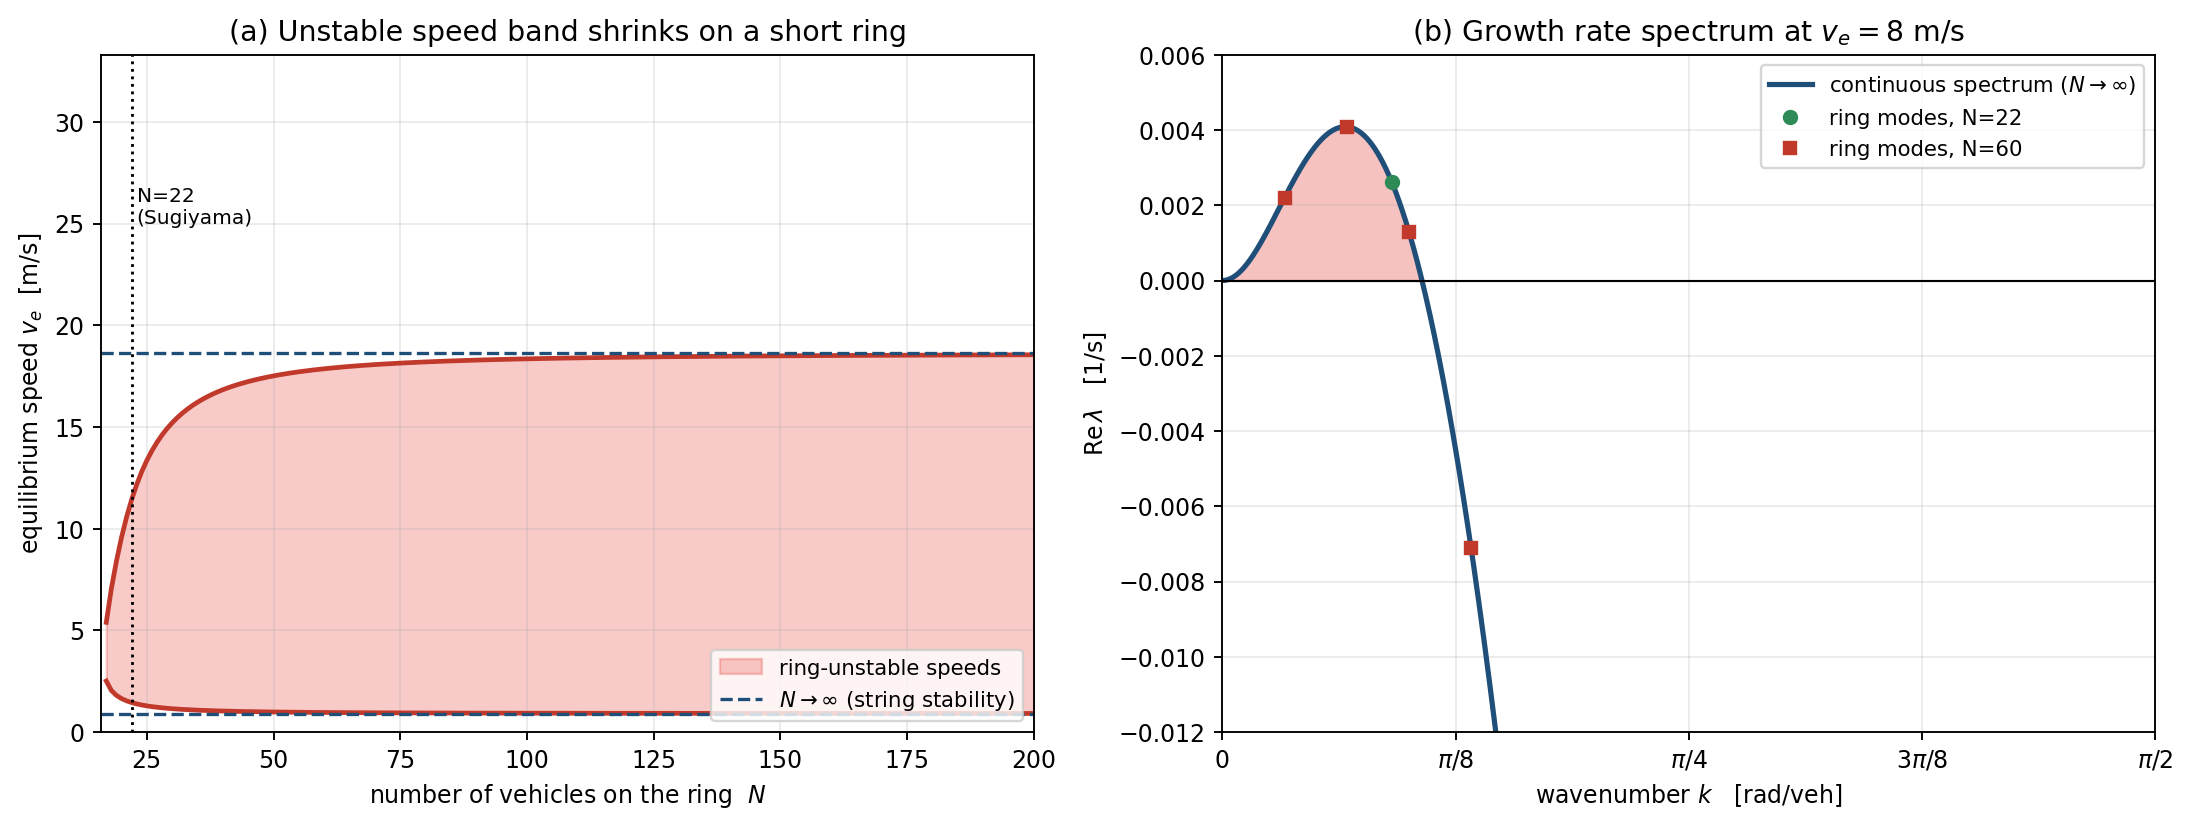
\includegraphics[width=\textwidth]{fig3.png}
\caption{有限环道规模对离散失稳模态的影响。}
\label{fig:finite-ring-band}
\figurenote{有限环道规模如何改变可观测失稳带。左图把车辆数 $N$ 从很小的环道逐步增加，实色边界给出每个有限 $N$ 的不稳定速度区间，虚线是 $N\to\infty$ 的线稳定极限；小环道的区间显著收缩，$N\le15$ 在本参数下甚至显示全速域稳定。右图固定 $v_e=8$ m/s，连续曲线是允许任意波数时的增长率谱，离散标记是特定环道真正能够取到的 $k_m=2\pi m/N$；危险正增长区只位于很窄的小 $k$ 范围。$N=22$ 的最低模态刚接近正增长区边缘，因此它只能捕捉无限车队失稳带的一部分；随着 $N$ 增大，离散点向零波数加密并逐渐复现连续谱。该图证明有限环道会因为采样不到长波而系统性高估稳定性，也说明实验车数必须作为稳定性结果的一部分报告。}
\end{figure}

\begin{tcolorbox}[notebox,title=\textbf{实用提醒}]
用有限环道仿真标定线稳定阈值会\textbf{系统性高估稳定性}。$N=22$（Sugiyama 经典实验的规模）算出的不稳定带只有真实值的一半多一点。要逼近线稳定性，$N$ 至少要上百。
\end{tcolorbox}

\begin{tcolorbox}[resultbox,title=\textbf{数值验证 E5：有限环道扫描}]
按 $N=5,10,15,22,50,100$ 逐一计算离散谱，得到的不稳定带依次为：全速域稳定、全速域稳定、全速域稳定、$1.45$--$11.43$、$0.99$--$17.51$、$0.93$--$18.35$ m/s；连续极限为 $0.91$--$18.61$ m/s。结果与闭式条件中的 $\cos(2\pi/N)$ 一致，并量化了有限环道未能采样危险长波所造成的偏差。
\end{tcolorbox}

\section{两种方法怎么选}
\sectionstudy{synthesis}{两种方法怎么选}{swaroop1996,ploeg2014,feng2019}

\begin{center}
\small
\captionof{table}{传递函数与环道 Fourier 方法的比较。}
\label{tab:transfer-versus-ring}
\begin{tabular}{p{3.0cm}p{5.4cm}p{5.4cm}}
\toprule
& \textbf{传递函数 $\left\|G\right\|_\infty\le1$} & \textbf{环形 $+$ 空间 Fourier} \\
\midrule
适用范围 & 仅限单向级联耦合 & 任意耦合结构（含双向、多前车） \\[4pt]
边界条件 & 开链，有一个领队 & 周期边界 \\[4pt]
问的问题 & 固定时间频率下\textbf{沿空间}的放大倍数 & 固定空间波数下\textbf{随时间}的增长率 \\[4pt]
计算量 & 一个标量不等式，最简单 & 需复系数 Routh--Hurwitz（Bilharz） \\[4pt]
额外信息 & 逐车放大倍数、最危险频率 & 增长率 $\operatorname{Re}\lambda(k)$、最不稳定波数（可预测走停波波长） \\
\bottomrule
\end{tabular}
\end{center}
\tabletext{tab:transfer-versus-ring}{两种稳定性方法的适用耦合、边界条件、问题类型和输出量。单向均匀车队中二者边界一致，但双向或多前车结构破坏标量级联后，只能使用环道色散关系或完整系统本征值。}

结论：\textbf{对单向模型，两种方法均成立，且在 $N\to\infty$ 时给出相同边界；传递函数计算更直接，环形分析适用范围更广，并能同时给出增长率与主导波数。} 一旦耦合变为双向，标量逐车传递函数不再适用，应转向环形或全系统本征值分析。

%==================================================================
\sectionwrapup{单向均匀车队中，环道条件 $G(\lambda)=e^{\mathrm{i}k}$ 把逐车传递和空间模态联系起来；当 $N\to\infty$ 时两者给出同一稳定边界。双向、异质或非局部耦合破坏标量级联后，应改用环道或全系统本征值。}

\backmatter
\setcounter{secnumdepth}{-1}
\renewcommand{\chaptermark}[1]{\markboth{#1}{}}
\renewcommand{\sectionmark}[1]{\markright{#1}}
\chapter{总结与展望}

\section{全部稳定性条件一览}
\sectionstudy{synthesis}{全部稳定性条件一览}{helbing2001,treiberkesting2013,ororsz2010}

\begin{center}
\scriptsize
\captionof{table}{基准及扩展模型的稳定性条件总览。}
\label{tab:all-stability-conditions}
\begin{tabular}{p{1.8cm}p{2.9cm}p{3.4cm}p{3.2cm}p{2.5cm}}
\toprule
& \textbf{基准模型} & \textbf{+ 前车加速度} & \textbf{+ 前后车加速度} & \textbf{+ 时间延迟} \\
\midrule
耦合结构 & 单向级联 & 单向级联 & \textbf{双向（三对角）} & 任意 \\[3pt]
$P(k)$ & $1$ & $1-f_ae^{-ik}$ & $1-f_ae^{-ik}-f_be^{ik}$ & 同左，另乘时滞因子 \\[3pt]
特征方程 & 二次（实根式） & 二次（复系数） & 二次（复系数） & \textbf{拟多项式} \\[3pt]
局部稳定 & $f_s>0,\ f_v<0$ & 完全相同 & 完全相同 & 新增 $\tau_0<\tau_0^{\rm crit}$ \\[3pt]
波速 $c_1$ & $V'(s_e)$ & 不变 & 不变 & 不变 \\[3pt]
长波条件 & $\dfrac{f_v^2-f_{v_l}^2}{2}\ge f_s$
        & $\dfrac{f_v^2-f_{v_l}^2}{2}\ge(1-f_a)f_s$
        & $\dfrac{f_v^2-f_{v_l}^2}{2}\ge(1-\sigma_{\rm eff})f_s$
        & \textbf{与左侧完全相同} \\[10pt]
额外条件 & 无 & $\left|f_a\right|\le1$
        & $\left|\sigma_{\rm eff}\right|<1$ 及 $\widetilde W(u)>0$ 的内部检验
        & $\Psi(\omega)\ge0$ 全频段 \\[8pt]
可用方法 & 长波 $=$ 传递函数 & \textbf{必须}传递函数 & \textbf{须}环形 $+$ Bilharz & 长波闭式 $+$ 数值 \\
\bottomrule
\end{tabular}
\end{center}
\tabletext{tab:all-stability-conditions}{基准模型、前车反馈、双向反馈和时间延迟在耦合结构、特征方程、局部／长波条件及额外约束上的对应关系。它可作为全书判据索引，但不能替代各章对有限波长与延迟全频段条件的推导。}

\section{异质车队（第~\ref{sec:het}~章）}
\sectionstudy{theory}{异质车队（第~\ref{sec:het}~章）}{helbing2001,treiberkesting2013,ororsz2010}

\begin{tcolorbox}[keybox]
\begin{itemize}[leftmargin=1.6em,itemsep=4pt]
\item 平衡态改为\textbf{同速不同距}；空间 Fourier 失效，传递函数成为唯一好用的工具（与双向耦合正相反）。
\item 链式乘积 $\hat y_j/\hat y_0=\prod_{n\le j}G_n$；环道特征方程为 $\prod_{n=1}^N G_n(\lambda)=1$。
\item 长波条件变成\textbf{加权前缀和} $\sum_{n\le j}\eta_n\ge0$，权重 $1/f_s^2$——迟钝的车（$f_s$ 小）权重极大。
\item \textbf{环道闭合只检查 $j=N$，开放车队内部无放大则检查所有 $j$}：固定 $G_n$ 时整圈乘积与排序无关，中途前缀增益却强烈依赖排序。
\item 本例混合自动驾驶：$\kappa=0.5$ 时整队／环道长波总预算门槛为 $26.7\%$，且与 $\kappa$ 近似成反比；该数字本身不保证任意排列满足前缀条件。
\item 若 AV 的前馈能力\textbf{取决于前车类型}（V2V 需前车也是 AV），则 $\eta_n$ 依赖相邻对，\textbf{连总和都变得依赖排序}：逐辆分散需 $89.1\%$ 渗透，成组编队只需 $26.7\%$。最优解是取满足 $n_{\rm grp}\le n_{\rm grp}^{\max}$ 的\textbf{最大组数}——先保长波预算，再尽量分散。
\end{itemize}
\end{tcolorbox}

\section{三个关键的"不变量"}
\sectionstudy{synthesis}{三个关键的"不变量"}{helbing2001,treiberkesting2013,ororsz2010}

\begin{tcolorbox}[keybox]
\begin{enumerate}[leftmargin=1.6em,itemsep=4pt]
\item \textbf{局部稳定性不受本书所考虑的邻车加速度反馈影响。} 前后车匀速时这些项恒为零，纯前馈不进入自车闭环；反应延迟则会为局部稳定性引入额外上限。
\item \textbf{加速度反馈不改变运动学波速。} 在 第~\ref{sec:lead}~章--第~\ref{sec:multi}~章 中始终有 $c_1=V'(s_e)$；后向间距反馈（第~\ref{sec:reargap}~章）则给出 $c_1=(1-h_s/f_s)V'$，并在完全对称极限下趋于零。
\item \textbf{长波门槛仅由零阶矩 $m_0$ 决定。} 在本书模型框架内，前视／回望的空间分配、观测车辆数与延迟均不改变这一门槛。因此，控制设计可先确定总增益预算，再检查有限波长与延迟约束。
\end{enumerate}
\end{tcolorbox}

\section{IDM 算例的数字汇总}
\sectionstudy{experiment}{IDM 算例的数字汇总}{treiber2000,treiberkesting2013}

参数：$v_0=33.3$ m/s，$T=1.5$ s，$s_0=2$ m，$a=1$ m/s$^2$，$b=1.5$ m/s$^2$，$\delta=4$，$l=5$ m。

\begin{center}
\small
\captionof{table}{基准 IDM 算例的关键数值。}
\label{tab:idm-number-summary}
\begin{tabular}{p{6.4cm}p{7.4cm}}
\toprule
基准不稳定速度带 & $0.91$ -- $18.61$ m/s（$\rho=27.4$--$119.6$ veh/km） \\
最易失稳处 & $v_e\approx3.1$ m/s，$\Phi_{\min}=-0.027$ \\
拥堵极限判据 & $aT^2/s_0=1.125>1$，故 $v_e\to0$ 处反而稳定 \\
\midrule
前车加速度前馈临界增益 & $\kappa_c=0.134$（上界为 1，裕度充足） \\
多前车（$\alpha=0.8$）所需最近邻增益 & $f_a=0.027$，即摊薄 $1/(1-\alpha)$ 倍 \\
纯回望可用窗口（$f_b>0,\beta=0$） & $0.134\le f_b\le0.43$；$\beta\gtrsim0.58$ 后无解 \\
\midrule
反应延迟：局部稳定上限 & $\tau_0^{\rm crit}=1.16$ s（$v_e=2$）$\sim$ $2.52$ s（$v_e=20$） \\
反应延迟拓宽不稳定带 & $\tau_0=1.5$ s 时扩至 $0$--$25.98$ m/s \\
通信延迟压缩增益窗口 & $\tau_a=1.5$ s 时 $\kappa$ 上界由 $1.00$ 降至 $0.60$，下界恒为 $0.134$ \\
\midrule
后向间距反馈临界权重 & $p_c=0.223$（$h_s=pf_s,\ h_v=pf_{v_l}$） \\
有限环道 $N=22$ 的不稳定带 & $1.45$--$11.43$ m/s（真值的一半多） \\
\bottomrule
\end{tabular}
\end{center}
\tabletext{tab:idm-number-summary}{基准 IDM 的不稳定速度带、反馈临界增益、延迟窗口、后视阈值和有限环道偏差。该表把分散在各章的代表性数字汇总到同一处，具体定义、适用条件和复现实验仍应回查相应章节。}

\section{非线性、学习型模型与应用结论}
\sectionstudy{application}{非线性、学习型模型与应用结论}{ororsz2010,wang2025kidl,chang2019neural}

\begin{tcolorbox}[keybox]
\begin{itemize}[leftmargin=1.5em,itemsep=4pt]
\item 原始 IDM 在中性线附近的统一弱非线性正规形是 Gardner--Burgers 型：扩散系数的符号由线性长波裕度决定，二次／三次非线性决定波形陡化，$O(k^3)$ 项提供色散。
\item 基准 IDM 的两个中性边界均不严格满足 $V''=0$，所以纯 mKdV 不是通用结论；下边界 $V''$ 很小，使用 Gardner 方程比直接丢掉二次项更稳妥。
\item $v_e=8$ m/s、$m=4$ 的 $0.02$ m/s 小扰动在 1800 s 内把 $\sigma_v$ 从 $0.01414$ 放大到 $2.962$ m/s，并出现明显波形陡化；$v_e=20$ m/s 的同一扰动则降到 $3.27\times10^{-8}$ m/s。
\item NGSIM US--101 的 D01 从 39187 条记录提取 78 个连续跟驰片段：中位经验增益为 $1.033$，但自助抽样 95\% 区间 $[0.954,1.077]$ 跨过 1，说明真实片段中放大与衰减并存，不能把单个时空图直接当成总体失稳证明。
\item D02 把真实数据应用推进到“标定--验证--优化”闭环：相较只拟合一辆跟随车，车队稳定性标定把留出段速度／间距 RMSE 分别降低 $69.6\%$ 与 $34.4\%$；随后由最不利经验速度下的谱约束选得 $\kappa=0.04$。该控制收益是标定模型上的反事实结果，不等同于真实道路已验证收益。
\item 稳定性分析可直接服务于 CACC 增益、AV 渗透率／编组、在线预警、环道规模、参数标定和鲁棒运行设计；应用时必须同时检查局部根、传播放大、有限幅响应与数值收敛。
\item 学习型跟驰器可由自动微分恢复平衡偏导；RNN／GNN 需扩充隐状态或全图雅可比，强化学习策略则必须连同车辆、观测、延迟与饱和检查完整闭环。训练收敛、低 RMSE 和高奖励均不能单独构成交通流稳定证据。
\end{itemize}
\end{tcolorbox}

\newpage
\section{工程要点}
\sectionstudy{theory}{工程要点}{helbing2001,treiberkesting2013,ororsz2010}

\begin{itemize}[leftmargin=1.4em,itemsep=4pt]
\item \textbf{先定总预算，再定分配。} 用长波条件算出所需的 $\sigma_{\rm eff}$（本例 $0.134$），这一步与延迟、分摊、前后分配全都无关。
\item \textbf{向前分配不降低长波裕度，向后分配需额外检查有限波长。} 前视方向的最近邻增益可按 $(1-\alpha)$ 线性下降；在本算例的正回望约定下，$\beta$ 不宜超过约 $0.5$。若采用文献中常见的负回望约定，结论会相应改变（\S\ref{sub:negfb}）。
\item \textbf{延迟不改变长波门槛，但会压缩可用增益区间。} 在本组参数附近，通信延迟每增加约 $0.5$ s，可用增益上界下降约 $0.1$--$0.2$；反应延迟通常更不利，而 $\tau_a\approx\tau_0$ 时部分相位效应可能抵消。
\item \textbf{稳定化与波速调节是两个不同目标。} 加速度反馈可以提高稳定裕度，但不改变 $c_1$；后向间距反馈同时影响二者。本例 $p_c=0.223$ 表示不稳定速度带刚好闭合，此时 $c_1=(1-p_c)V'$ 仍非零；只有在完全对称极限 $p\to1$ 时波速才趋于零。
\item \textbf{别用短环道标定阈值。} $N=22$ 会系统性高估稳定性，要逼近线稳定性 $N$ 至少上百。
\end{itemize}

\section{适用范围与后续}
\sectionstudy{synthesis}{适用范围与后续}{helbing2001,treiberkesting2013,ororsz2010}

\begin{tcolorbox}[notebox]
第~\ref{sec:nonlinear}~章已经把原始 IDM 推进到\textbf{弱非线性}层级，能够解释中性线附近的扩散、色散、波形陡化以及 KdV／mKdV／Gardner 约化条件；但本书仍不声称给出了任意有限幅扰动下的全局稳定性证明。尚未覆盖的问题包括：
\begin{itemize}[leftmargin=1.2em,itemsep=2pt]
\item 用双向延续或分岔软件严格定位有限幅扰动下的\textbf{亚临界分岔}、共存吸引子与迟滞环；
\item 为含前馈、回望、时间延迟和异质性的模型重新推导各自的非线性正规形；
\item 换道、匝道、随机驾驶、通信丢包与离散控制器共同作用下的稳定性；
\item 将非线性幅宽关系与实测轨迹数据作系统统计检验，而不只作单组仿真对照。
\item 把第~\ref{sec:ml-stability}~章的局部雅可比诊断推进到含模型误差、随机策略和大规模注意力网络的可扩展闭环认证。
\end{itemize}
这些问题需要全系统数值延续、随机稳定性或混杂系统工具，超出本书的单车道确定性框架。
\end{tcolorbox}

\section{全书小结}
\sectionstudy{synthesis}{全书小结}{helbing2001,treiberkesting2013,ororsz2010}

本书形成了从单车局部根、车队传递、环道模态、有限幅波形到宏观连续流、学习型动力学和工程控制的完整层级。使用任何“稳定”结论时，都应同时说明模型或网络架构、平衡工况、扰动尺度、边界条件、允许波数、采样方式和数值精度；只有这些条件一致，理论判据、仿真图像、数据证据和交通管理含义才可相互验证。

\clearpage
\begin{thebibliography}{99}
\bibitem{chandler1958}
Robert E. Chandler, Robert Herman, and Elliott W. Montroll,
{Traffic dynamics: Studies in car following},
\emph{Operations Research}, vol.~6, no.~2, pp.~165--184, 1958.
\href{https://doi.org/10.1287/opre.6.2.165}{doi:10.1287/opre.6.2.165}.

\bibitem{gazis1961}
Denos C. Gazis, Robert Herman, and Richard W. Rothery,
{Nonlinear follow-the-leader models of traffic flow},
\emph{Operations Research}, vol.~9, no.~4, pp.~545--567, 1961.
\href{https://doi.org/10.1287/opre.9.4.545}{doi:10.1287/opre.9.4.545}.

\bibitem{bando1995}
Masako Bando, Katsuya Hasebe, Akihiro Nakayama, Akihiro Shibata, and Yuki Sugiyama,
{Dynamical model of traffic congestion and numerical simulation},
\emph{Physical Review E}, vol.~51, no.~2, pp.~1035--1042, 1995.
\href{https://doi.org/10.1103/PhysRevE.51.1035}{doi:10.1103/PhysRevE.51.1035}.

\bibitem{treiber2000}
Martin Treiber, Ansgar Hennecke, and Dirk Helbing,
{Congested traffic states in empirical observations and microscopic simulations},
\emph{Physical Review E}, vol.~62, no.~2, pp.~1805--1824, 2000.
\href{https://doi.org/10.1103/PhysRevE.62.1805}{doi:10.1103/PhysRevE.62.1805}.

\bibitem{lighthill1955}
M. J. Lighthill and G. B. Whitham,
``On kinematic waves II. A theory of traffic flow on long crowded roads,''
\emph{Proceedings of the Royal Society A}, vol.~229, no.~1178, pp.~317--345, 1955.
\href{https://doi.org/10.1098/rspa.1955.0089}{doi:10.1098/rspa.1955.0089}.

\bibitem{richards1956}
Paul I. Richards,
``Shock waves on the highway,''
\emph{Operations Research}, vol.~4, no.~1, pp.~42--51, 1956.
\href{https://doi.org/10.1287/opre.4.1.42}{doi:10.1287/opre.4.1.42}.

\bibitem{payne1971}
Harold J. Payne,
``Models of freeway traffic and control,''
in \emph{Mathematical Models of Public Systems}, vol.~1, pp.~51--61, 1971.

\bibitem{daganzo1995}
Carlos F. Daganzo,
``Requiem for second-order fluid approximations of traffic flow,''
\emph{Transportation Research Part B: Methodological}, vol.~29, no.~4, pp.~277--286, 1995.
\href{https://doi.org/10.1016/0191-2615(95)00007-Z}{doi:10.1016/0191-2615(95)00007-Z}.

\bibitem{awrascle2000}
Awatif Aw and Michel Rascle,
``Resurrection of `second order' models of traffic flow,''
\emph{SIAM Journal on Applied Mathematics}, vol.~60, no.~3, pp.~916--938, 2000.
\href{https://doi.org/10.1137/S0036139997332099}{doi:10.1137/S0036139997332099}.

\bibitem{zhang2002}
H. Michael Zhang,
``A non-equilibrium traffic model devoid of gas-like behavior,''
\emph{Transportation Research Part B: Methodological}, vol.~36, no.~3, pp.~275--290, 2002.
\href{https://doi.org/10.1016/S0191-2615(00)00050-3}{doi:10.1016/S0191-2615(00)00050-3}.

\bibitem{jin2003}
Wen-Long Jin and H. Michael Zhang,
``The formation and structure of vehicle clusters in the Payne--Whitham traffic flow model,''
\emph{Transportation Research Part B: Methodological}, vol.~37, no.~3, pp.~207--223, 2003.
\href{https://doi.org/10.1016/S0191-2615(02)00008-5}{doi:10.1016/S0191-2615(02)00008-5}.

\bibitem{ngsim2016}
U.S. Department of Transportation, Federal Highway Administration,
\emph{Next Generation Simulation (NGSIM) Vehicle Trajectories and Supporting Data},
dataset, 2016, accessed 2026-08-28.
\href{https://doi.org/10.21949/1504477}{doi:10.21949/1504477}.

\bibitem{savitzky1964}
Abraham Savitzky and Marcel J. E. Golay,
``Smoothing and differentiation of data by simplified least squares procedures,''
\emph{Analytical Chemistry}, vol.~36, no.~8, pp.~1627--1639, 1964.
\href{https://doi.org/10.1021/ac60214a047}{doi:10.1021/ac60214a047}.

\bibitem{wu2015ev}
Xinkai Wu, David Freese, Alfredo Cabrera, and William A. Kitch,
``Electric vehicles' energy consumption measurement and estimation,''
\emph{Transportation Research Part D: Transport and Environment}, vol.~34, pp.~52--67, 2015.
\href{https://doi.org/10.1016/j.trd.2014.10.007}{doi:10.1016/j.trd.2014.10.007}.

\bibitem{newell1961}
Gordon F. Newell,
``Nonlinear effects in the dynamics of car following,''
\emph{Operations Research}, vol.~9, no.~2, pp.~209--229, 1961.
\href{https://doi.org/10.1287/opre.9.2.209}{doi:10.1287/opre.9.2.209}.

\bibitem{gipps1981}
Peter G. Gipps,
``A behavioural car-following model for computer simulation,''
\emph{Transportation Research Part B: Methodological}, vol.~15, no.~2, pp.~105--111, 1981.
\href{https://doi.org/10.1016/0191-2615(81)90037-0}{doi:10.1016/0191-2615(81)90037-0}.

\bibitem{jiang2001}
Rui Jiang, Qing-Song Wu, and Zuo-Jin Zhu,
``Full velocity difference model for a car-following theory,''
\emph{Physical Review E}, vol.~64, 017101, 2001.
\href{https://doi.org/10.1103/PhysRevE.64.017101}{doi:10.1103/PhysRevE.64.017101}.

\bibitem{helbing2001}
Dirk Helbing,
``Traffic and related self-driven many-particle systems,''
\emph{Reviews of Modern Physics}, vol.~73, no.~4, pp.~1067--1141, 2001.
\href{https://doi.org/10.1103/RevModPhys.73.1067}{doi:10.1103/RevModPhys.73.1067}.

\bibitem{treiberkesting2013}
Martin Treiber and Arne Kesting,
\emph{Traffic Flow Dynamics: Data, Models and Simulation},
Springer, Berlin, 2013.
\href{https://doi.org/10.1007/978-3-642-32460-4}{doi:10.1007/978-3-642-32460-4}.

\bibitem{wilsonward2011}
R. Eddie Wilson and Jonathan A. Ward,
``Car-following models: Fifty years of linear stability analysis---a mathematical perspective,''
\emph{Transportation Planning and Technology}, vol.~34, no.~1, pp.~3--18, 2011.
\href{https://doi.org/10.1080/03081060.2011.530826}{doi:10.1080/03081060.2011.530826}.

\bibitem{swaroop1996}
D. Swaroop and J. Karl Hedrick,
``String stability of interconnected systems,''
\emph{IEEE Transactions on Automatic Control}, vol.~41, no.~3, pp.~349--357, 1996.
\href{https://doi.org/10.1109/9.486636}{doi:10.1109/9.486636}.

\bibitem{ploeg2014}
Jeroen Ploeg, Nathan van de Wouw, and Henk Nijmeijer,
``$L_p$ string stability of cascaded systems: Application to vehicle platooning,''
\emph{IEEE Transactions on Control Systems Technology}, vol.~22, no.~2, pp.~786--793, 2014.
\href{https://doi.org/10.1109/TCST.2013.2258346}{doi:10.1109/TCST.2013.2258346}.

\bibitem{stuedli2017}
Sonja St\"udli, María M. Seron, and Richard H. Middleton,
``From vehicular platoons to general networked systems: String stability and related concepts,''
\emph{Annual Reviews in Control}, vol.~44, pp.~157--172, 2017.
\href{https://doi.org/10.1016/j.arcontrol.2017.09.016}{doi:10.1016/j.arcontrol.2017.09.016}.

\bibitem{feng2019}
Shuo Feng, Yi Zhang, Shengbo Eben Li, Zhong Cao, Henry X. Liu, and Li Li,
``String stability for vehicular platoon control: Definitions and analysis methods,''
\emph{Annual Reviews in Control}, vol.~47, pp.~81--97, 2019.
\href{https://doi.org/10.1016/j.arcontrol.2019.03.001}{doi:10.1016/j.arcontrol.2019.03.001}.

\bibitem{dunbar2012}
William B. Dunbar and Derek S. Caveney,
``Distributed receding horizon control of vehicle platoons: Stability and string stability,''
\emph{IEEE Transactions on Automatic Control}, vol.~57, no.~3, pp.~620--633, 2012.
\href{https://doi.org/10.1109/TAC.2011.2159651}{doi:10.1109/TAC.2011.2159651}.

\bibitem{ororsz2004}
Gábor Orosz, R. Eddie Wilson, and Bernd Krauskopf,
``Global bifurcation investigation of an optimal velocity traffic model with driver reaction time,''
\emph{Physical Review E}, vol.~70, 026207, 2004.
\href{https://doi.org/10.1103/PhysRevE.70.026207}{doi:10.1103/PhysRevE.70.026207}.

\bibitem{ororsz2010}
Gábor Orosz, R. Eddie Wilson, and Gábor Stépán,
``Traffic jams: Dynamics and control,''
\emph{Philosophical Transactions of the Royal Society A}, vol.~368, no.~1928, pp.~4455--4479, 2010.
\href{https://doi.org/10.1098/rsta.2010.0205}{doi:10.1098/rsta.2010.0205}.

\bibitem{lenz1999}
Hanno Lenz, Christian K. Wagner, and Ralf Sollacher,
``Multi-anticipative car-following model,''
\emph{The European Physical Journal B}, vol.~7, no.~2, pp.~331--335, 1999.
\href{https://doi.org/10.1007/s100510050618}{doi:10.1007/s100510050618}.

\bibitem{sugiyama2008}
Yuki Sugiyama, Minoru Fukui, Macoto Kikuchi, Katsuya Hasebe, Akihiro Nakayama,
Katsuhiro Nishinari, Shin-ichi Tadaki, and Satoshi Yukawa,
``Traffic jams without bottlenecks---experimental evidence for the physical mechanism of the formation of a jam,''
\emph{New Journal of Physics}, vol.~10, 033001, 2008.
\href{https://doi.org/10.1088/1367-2630/10/3/033001}{doi:10.1088/1367-2630/10/3/033001}.

\bibitem{treiberkesting2011}
Martin Treiber and Arne Kesting,
``Evidence of convective instability in congested traffic flow: A systematic empirical and theoretical investigation,''
\emph{Transportation Research Part B: Methodological}, vol.~45, no.~9, pp.~1362--1377, 2011.
\href{https://doi.org/10.1016/j.trb.2011.05.011}{doi:10.1016/j.trb.2011.05.011}.

\bibitem{milanes2014}
Vicente Milanés, Steven E. Shladover, John Spring, Christopher Nowakowski,
Hiroshi Kawazoe, and Masahide Nakamura,
``Cooperative adaptive cruise control in real traffic situations,''
\emph{IEEE Transactions on Intelligent Transportation Systems}, vol.~15, no.~1, pp.~296--305, 2014.
\href{https://doi.org/10.1109/TITS.2013.2278494}{doi:10.1109/TITS.2013.2278494}.

\bibitem{talebpour2016}
Alireza Talebpour and Hani S. Mahmassani,
``Influence of connected and autonomous vehicles on traffic flow stability and throughput,''
\emph{Transportation Research Part C: Emerging Technologies}, vol.~71, pp.~143--163, 2016.
\href{https://doi.org/10.1016/j.trc.2016.07.007}{doi:10.1016/j.trc.2016.07.007}.

\bibitem{stern2018}
Raphael E. Stern, Shumo Cui, Maria Laura Delle Monache, Rahul Bhadani,
Matt Bunting, Miles Churchill, et al.,
``Dissipation of stop-and-go waves via control of autonomous vehicles: Field experiments,''
\emph{Transportation Research Part C: Emerging Technologies}, vol.~89, pp.~205--221, 2018.
\href{https://doi.org/10.1016/j.trc.2018.02.005}{doi:10.1016/j.trc.2018.02.005}.

\bibitem{komatsu1995}
Teruhisa S. Komatsu and Shin-ichi Sasa,
``A kink soliton characterizing traffic congestion,''
\emph{Physical Review E}, vol.~52, no.~5, pp.~5574--5582, 1995.
\href{https://doi.org/10.1103/PhysRevE.52.5574}{doi:10.1103/PhysRevE.52.5574}.

\bibitem{leveque2002}
Randall J. LeVeque,
\emph{Finite Volume Methods for Hyperbolic Problems},
Cambridge University Press, Cambridge, 2002.
\href{https://doi.org/10.1017/CBO9780511791253}{doi:10.1017/CBO9780511791253}.

\bibitem{kesting2008}
Arne Kesting and Martin Treiber,
``Calibrating car-following models by using trajectory data: Methodological study,''
\emph{Transportation Research Record}, no.~2088, pp.~148--156, 2008.
\href{https://doi.org/10.3141/2088-16}{doi:10.3141/2088-16}.

\bibitem{ossen2009}
Saskia Ossen and Serge P. Hoogendoorn,
``Reliability of parameter values estimated using trajectory observations,''
\emph{Transportation Research Record}, no.~2124, pp.~36--44, 2009.
\href{https://doi.org/10.3141/2124-04}{doi:10.3141/2124-04}.

\bibitem{punzo2012}
Vincenzo Punzo, Biagio Ciuffo, and Marcello Montanino,
``Can results of car-following model calibration based on trajectory data be trusted?''
\emph{Transportation Research Record}, no.~2315, pp.~11--24, 2012.
\href{https://doi.org/10.3141/2315-02}{doi:10.3141/2315-02}.

\bibitem{thiemann2008}
Christian Thiemann, Martin Treiber, and Arne Kesting,
``Estimating acceleration and lane-changing dynamics from Next Generation Simulation trajectory data,''
\emph{Transportation Research Record}, no.~2088, pp.~90--101, 2008.
\href{https://doi.org/10.3141/2088-10}{doi:10.3141/2088-10}.

\bibitem{krajewski2018}
Robert Krajewski, Julian Bock, Laurent Kloeker, and Lutz Eckstein,
``The highD dataset: A drone dataset of naturalistic vehicle trajectories on German highways for validation of highly automated driving systems,''
in \emph{2018 IEEE 21st International Conference on Intelligent Transportation Systems}, pp.~2118--2125, 2018.
\href{https://doi.org/10.1109/ITSC.2018.8569552}{doi:10.1109/ITSC.2018.8569552}.

\bibitem{hegyi2005}
Andreas Hegyi, Bart De Schutter, and J. Hellendoorn,
``Optimal coordination of variable speed limits to suppress shock waves,''
\emph{IEEE Transactions on Intelligent Transportation Systems}, vol.~6, no.~1, pp.~102--112, 2005.
\href{https://doi.org/10.1109/TITS.2004.842408}{doi:10.1109/TITS.2004.842408}.

\bibitem{carlson2010}
Rodrigo C. Carlson, Ioannis Papamichail, Markos Papageorgiou, and Albert Messmer,
``Optimal motorway traffic flow control involving variable speed limits and ramp metering,''
\emph{Transportation Science}, vol.~44, no.~2, pp.~238--253, 2010.
\href{https://doi.org/10.1287/trsc.1090.0314}{doi:10.1287/trsc.1090.0314}.

\bibitem{chen2018neuralode}
Ricky T. Q. Chen, Yulia Rubanova, Jesse Bettencourt, and David K. Duvenaud,
``Neural ordinary differential equations,''
in \emph{Advances in Neural Information Processing Systems 31}, pp.~6571--6583, 2018.
\href{https://proceedings.neurips.cc/paper/2018/hash/69386f6bb1dfed68692a24c8686939b9-Abstract.html}{NeurIPS proceedings}.

\bibitem{bai2019deq}
Shaojie Bai, J. Zico Kolter, and Vladlen Koltun,
``Deep equilibrium models,''
in \emph{Advances in Neural Information Processing Systems 32}, 2019.
\href{https://proceedings.neurips.cc/paper/2019/hash/01386bd6d8e091c2ab4c7c7de644d37b-Abstract.html}{NeurIPS proceedings}.

\bibitem{miyato2018spectral}
Takeru Miyato, Toshiki Kataoka, Masanori Koyama, and Yuichi Yoshida,
``Spectral normalization for generative adversarial networks,''
in \emph{International Conference on Learning Representations}, 2018.
\href{https://arxiv.org/abs/1802.05957}{arXiv:1802.05957}.

\bibitem{revay2020contracting}
Max Revay and Ian Manchester,
``Contracting implicit recurrent neural networks: Stable models with improved trainability,''
in \emph{Proceedings of the 2nd Conference on Learning for Dynamics and Control},
PMLR, vol.~120, pp.~393--403, 2020.
\href{https://proceedings.mlr.press/v120/revay20a.html}{PMLR:120:393--403}.

\bibitem{chang2019neural}
Ya-Chien Chang, Nima Roohi, and Sicun Gao,
``Neural Lyapunov control,''
in \emph{Advances in Neural Information Processing Systems 32}, pp.~3240--3249, 2019.
\href{https://proceedings.neurips.cc/paper/2019/hash/2647c1dba23bc0e0f9cdf75339e120d2-Abstract.html}{NeurIPS proceedings}.

\bibitem{fazlyab2022}
Mahyar Fazlyab, Manfred Morari, and George J. Pappas,
``Safety verification and robustness analysis of neural networks via quadratic constraints and semidefinite programming,''
\emph{IEEE Transactions on Automatic Control}, vol.~67, no.~1, pp.~1--15, 2022.
\href{https://doi.org/10.1109/TAC.2020.3046193}{doi:10.1109/TAC.2020.3046193}.

\bibitem{raissi2019pinn}
Maziar Raissi, Paris Perdikaris, and George E. Karniadakis,
``Physics-informed neural networks: A deep learning framework for solving forward and inverse problems involving nonlinear partial differential equations,''
\emph{Journal of Computational Physics}, vol.~378, pp.~686--707, 2019.
\href{https://doi.org/10.1016/j.jcp.2018.10.045}{doi:10.1016/j.jcp.2018.10.045}.

\bibitem{brunton2016sindy}
Steven L. Brunton, Joshua L. Proctor, and J. Nathan Kutz,
``Discovering governing equations from data by sparse identification of nonlinear dynamical systems,''
\emph{Proceedings of the National Academy of Sciences}, vol.~113, no.~15, pp.~3932--3937, 2016.
\href{https://doi.org/10.1073/pnas.1517384113}{doi:10.1073/pnas.1517384113}.

\bibitem{lusch2018koopman}
Bethany Lusch, J. Nathan Kutz, and Steven L. Brunton,
``Deep learning for universal linear embeddings of nonlinear dynamics,''
\emph{Nature Communications}, vol.~9, 4950, 2018.
\href{https://doi.org/10.1038/s41467-018-07210-0}{doi:10.1038/s41467-018-07210-0}.

\bibitem{kreidieh2018drl}
Abdul Rahman Kreidieh, Cathy Wu, and Alexandre M. Bayen,
``Dissipating stop-and-go waves in closed and open networks via deep reinforcement learning,''
in \emph{2018 IEEE 21st International Conference on Intelligent Transportation Systems}, pp.~1475--1480, 2018.
\href{https://doi.org/10.1109/ITSC.2018.8569485}{doi:10.1109/ITSC.2018.8569485}.

\bibitem{wang2025kidl}
Chengming Wang, Dongyao Jia, Wei Wang, Dong Ngoduy, Bei Peng, and Jianping Wang,
``A knowledge-informed deep learning paradigm for generalizable and stability-optimized car-following models,''
\emph{Communications in Transportation Research}, vol.~5, 100211, 2025.
\href{https://doi.org/10.1016/j.commtr.2025.100211}{doi:10.1016/j.commtr.2025.100211}.
\end{thebibliography}

\end{document}
